% -*- TeX-master: "Qualificacao.tex" -*-
%!TEX root = Qualificacao.tex

%%%%%%%%%%%%%%%%%%%%%%%%%%%%%%%%%%%%%%%%%%%%%%%%%%%%%%%%%%%%%%%%%
%  CHAPTER 3 - VIRTUAL REFERENCE FEEDBACK TUNNING  ( V R F T )  %
%%%%%%%%%%%%%%%%%%%%%%%%%%%%%%%%%%%%%%%%%%%%%%%%%%%%%%%%%%%%%%%%%

\chapter{Virtual Reference Feedback Tuning}\label{cap:VRFT}
\vspace{-1cm}

% \section{Introdução}\label{sec:introvrft}

The \textit{Virtual Reference Feedback Tunning} method, or simply VRFT, proposed by \cite{campi2002}, is a procedure that aims to design closed loop controllers based only on data sampled from the process, without the need for a model that describes that process itself. Thus, it is classified as a data-based control method, or DDC.

The main objective of this method is to adjust the parameters of a controller, defined by a parametric function like \eqref{eq:uknl_par}, using the process sampled data only, so that the output signal of the controlled process, $y_\theta(k)$ behaves as close as possible to the output signal $\tilde{\bm{y}}$ of a previously defined reference model as defined in \eqref{eq:Mmap}.
To reach this objective, VRFT aims to optimize the tracking error by minimizing a performance index $J_{RM}^N(\vtheta)$ as stated in \eqref{eq:Jy}, rewritten here for convenience:
\begin{equation}
   J_{RM}^N(\bm{\theta}) \triangleq \lim_{N \to \infty}  \frac{1}{N} \sum_{k=1}^N \left[y(k,\vtheta) - \tilde{y}(k)\right]^2 = 
    \left\lVert y_\theta - \tilde{\bm{y}} \right\lVert^{2}
   \label{eq:Jy},
\end{equation}
where $N$ represents the number of data samples, $\vtheta = \begin{bmatrix} \theta_1 & \theta_2 & \cdots & \theta_N \end{bmatrix}^T \in \R^N$ a vector of parameters and $k$ a temporal index. The signal $y_\theta(k) \in \R $ represents the output of the  system controlled with the parametrized controller $C_\theta$, and $\tilde{y}(k) \in \mathbb{R}$ are the output of a reference model $M$, both subject to the same reference signal.

To achieve the objective of minimizing \eqref{eq:Jy}, \cite{campi2002}, for the linear case, and \cite{campi2006}, for the non-linear case, show that, under certain conditions, presented in sequence, when minimizing a cost index defined as
\begin{equation}
 J_{VR}^N(\vtheta) \triangleq \lim_{N \to \infty}  \frac{1}{N} \sum_{k=1}^N \left[u(k) - C_\theta(q,\vtheta)\bar{e}(k)\right]^2
   \label{eq:Jvr},
\end{equation}
% minimiza-se também o índice $J_{RM}(\theta)$ definido em ~\eqref{eq:Jy}. Em \eqref{eq:Jvr}, $u(k)$ representa o sinal de entrada aplicado ao processo durante a coleta de dados, $C(q,\vtheta)$ o modelo do controlador a ser ajustado e $e(k)$ é o chamado \textit{erro virtual}, definido como
the index $J_{RM}(\vtheta)$ defined in~\eqref{eq:Jy} is also minimized.

\textbf{Notation:} The symbol ``tilde'' will be adopted on the variables to indicate that they represent data obtained, or calculated, from the data collection experiment, used for the purpose of identifying the controller parameters.

According to the notation adopted, $\tilde{u}(k)$ em ~\eqref{eq:Jvr} represents the input signal applied to the process during data collection, $C (q,\vtheta)$ the controller model to be adjusted and $\tilde{e}(k)$ is the so-called \textit{virtual error}, defined as
\begin{equation}
   \tilde{e}(k) = \tilde{\bm{r}}(k) - \tilde{y}(k) 
   \label{eq:ev},
\end{equation}
where $\tilde{\bm{r}}(k)$ is a signal called \textit{virtual reference}, obtained by filtering the output $\tilde{y}(k)$ by the inverse of the reference model $M$ defined in  \eqref{eq:Mmap} and in \eqref{eq:Mq} for a linear case. So, for a linear reference model, the virtual reference can be defined as
\begin{equation}
   \tilde{\bm{r}}(k) = M^{-1}(q){\tilde{\bm{y}}}(k)
   \label{eq:refvirt}.
\end{equation}

The term, $\tilde{y}(k)$ in \eqref{eq:ev} and \eqref{eq:refvirt}, represents the sampled output signal used in the experiment.

Figure~\ref{fig:Figs-diagrama_VRFT-eps} shows a block diagram with the steps used in the experiment to obtain the controller parameters via the VRFT procedure.
\begin{figure}[H]
   \sbox0{\blacksolidline} \sbox1{\bluedashedline} \sbox2{\reddashedline}
   \centering
   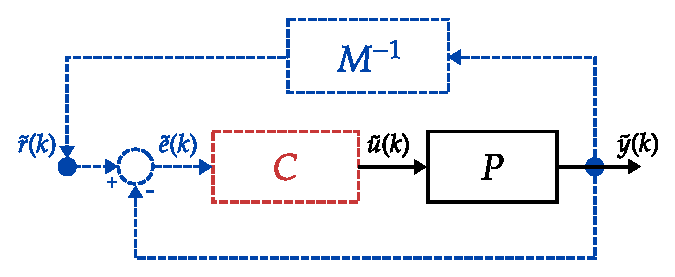
\includegraphics{Figs/diagrama_VRFT_maps.eps}
   % 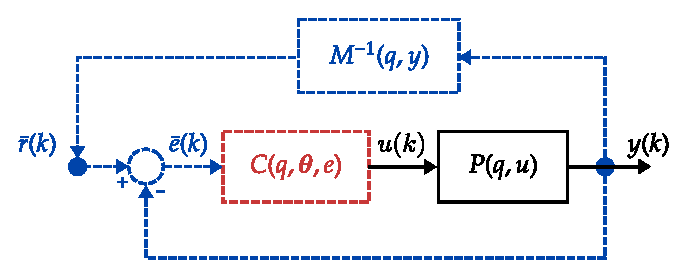
\includegraphics{Figs/diagrama_VRFT.eps}
   % \todo[inline]{Corrigir os termos na figura.}
   \caption{Experiment to obtain the data used to identify the controller parameters by the VRFT method: real data in \textit{black solid lines} (\usebox0), virtual data in \textit{blue dashed lines} (\usebox1) and the cotroller to tune, in \textit{red dashed block} (\usebox2).}
   \label{fig:Figs-diagrama_VRFT-eps}
\end{figure}
% onde $\tilde{\bm{r}}$ é o sinal de \textit{referência virtual}, obtido ao se filtrar a saída $y(k)$ pelo modelo de referência inverso, na forma
The term ``virtual'' is adopted in the reference $\tilde{\bm{r}}$ and in the tracking error $\tilde{\bm{e}}$ signals to emphasize that none of these signals are physically available, but only calculated for controller design purposes. 
The dashed lines (in blue) in Figure \ref{fig:Figs-diagrama_VRFT-eps} represent these virtual data, and the red block represents the controller under which the vector of parameters $\bm{\theta}$ need to be adjusted.

The condition for  $J_{RM}(\vtheta)$ and $J_{VR}(\vtheta)$ reach their minimum values for the same parameter solution $\vtheta$ are presented in sequence, right after some definitions and Assumptions that are important for the rest of the chapter.

\section{Initial Considerations}\label{sec:vrft_Init_Cons}
This Section presents some definitions and Assumptions used in the rest of the chapter.

\begin{assum}[The Process]
   It is assumed that the process is the one presented in Section \ref{sec:TheProcess} and therefore, it is a nonlinear process, assumed to be smooth (Assumption \ref{ass:psuave}) and invertible (Assumption \ref{ass:invert}).
\end{assum}

\begin{defn}[Ideal Controller]\label{def:idealControler}
   The ideal controller is defined as in the Section \ref{sec:ideal_controller} and is represented by the map $C_0 $, which maps $\tilde{\bm{e}}\mapsto \tilde{\bm{u}}$. For the linear case, the notation $C_0(q,\bm{\theta})$ is used for temporal representations or $C_0 (z,\bm{\theta})$ for transfer functions.
   % É o controlador que, quando colocado na malha fechada, resulta na mesma saída $\tilde{y}(k)$ que o modelo de referência $M$ (ou $M(q)$ e $M(z)$ para o caso linear), quand ambos estão sobre efeito do mesmo sinal de referência $\tilde{\bm{r}}$.
   % \todo[inline]{}
\end{defn}

Considering that a structure for the controller is previously chosen (i.e. if it is linear or not, how many parameters are considered, or what regressors are considered in construction), it is said that this structure is defined by a $\mathscr{C}$ class. That is, the $\mathscr{C}$ class represents all possible controllers using the same structure.
% COMTEMP \todo{Olhar se consigo colocar isso de maneira formal (equacao). Vide Bazanella.} 

\begin{assum}[Matched control]\label{ass:machedControl} %% Assumption By of \citep{bazanella2012} pg 13 
   The ideal controller belongs to control model class considered, i.e. $C_0(q) \in \mathscr{C}$, or, equivalently
   \begin{equation}
      \exists \bm{\theta}_0 : C(q,\bm{\theta}_0)=C_0(q)
      \label{eq:assumpMatched}.
   \end{equation}
\end{assum}

\begin{assum}[Noise free]
   \label{ass:noiseFree} 
   The system is considered to be not affected by noise.
\end{assum}
Unless otherwise noted, this chapter assumes that there are no measurement noise, that is, $\nu(k)$ is null and $y_{\nu}(k) = y(k)$ (see Figure \ref{fig:diagrama_MF}).

\begin{assum}[The asymptotic counterpart] \label{ass:asympCount}
   The measured signals $\tilde{u}(k)$ and $\tilde{y}(k)$ are considered realizations of stationary and ergodic stochastic processes so, when the number of available data grows $(N \to \infty)$, the following holds\footnote{The operator $\mathbb{E}[\cdot]^{2}$ represents the expected value operator of a quadratic random variable: $\mathbb{E}[\cdot]^{2} = \lim_{N\to \infty} \frac{1}{N}\sum_{k=1}^{N} \left( \cdot \right)^{2}$.}:
   $$ J_{\mathrm{VR}}^{N}(\theta) \rightarrow J_{\mathrm{VR}}(\theta)=\mathbb{E}\left[ \left(\tilde{\bm{u}}-C_\theta[\tilde{\bm{e}} ]\right)\right]^{2}, $$
   % COMTEMP \todo{Confirmar este quadrado na esperanca.} 
   so,  $J_{VR}$ is the \textit{asymptotic counterpart} of $J_{VR}^N$ and for the rest of text $J_{VR}$ will be used in place of $J_{VR}^N$ for analysis purposes.
\end{assum}

\begin{assum}[Linear parametrized controller] \label{ass:LPC}
   The controller is assumed to be linear in the parameters, as \eqref{eq:uknl_par}, and will be represented by the map $C_{\theta}$, or by $C_\theta(q, \bm{\theta}, \tilde{\bm{e}} )$, depending on the context. If it is linear, $C_\theta(q,\bm{\theta})$ is used as a function of time, or $C_\theta(z,\bm{\theta})$ when in the form of a transfer function.
\end{assum}

Note that, from Assumption~\ref{ass:LPC}, we can write the controller $C_\theta(q,\bm{\theta},\tilde{\bm{e}}) = \bm{\vvarphi}^{T}\bm{\theta}$, with $\bm{\vvarphi}$ being a vector of regressors as discussed in Section~\ref{sec:parest}. Thus, considering the Assumption~\ref{ass:asympCount}, we have
\begin{equation}
   J_{VR}(\bm{\theta}) = \frac{1}{N}\sum_{k=1}^{N} \left[ \tilde{u}(k) - \bm{\varphi}^{T}(k)\bm{\theta} \right]^{2} = \norm{\tilde{\bm{u}}-\Psi^T\bm{\theta}}^{2}
\label{eq:JVR_reg}
\end{equation}
where $\Psi$ the regressors matrix, as defined in the Section~\ref{sec:parest}, equation~\refeq{eq:yMatrix}.

\begin{defn}[SR$q$ process \citep{bazanella2012}] \label{def:SRq}
   A quasi-stationary process is said to be sufficiently rich of order $q$ -- or simply SR$q$ -- if its spectrum has at least $q$ nonzero components.
\end{defn}

\begin{defn}[Persistence of excitation \citep{bazanella2012}] \label{def:PoE}
   A quasi-stationary vector $\vvarphi$ is said to be persistently exciting if $\bar{\mathbb{E}}[\vvarphi(k)\vvarphi(k)^{T}] > 0$
\end{defn}
\todo{colocar uma Assumption que esta definição é satisfeita? Acho que basta a PoE que a SRq já se satisfaz.} 

\begin{assum}
   The signal $\tilde{\bm{u}}$ used in the excitation of process $P$ is persistently exciting (definition \label{def:PoE}), which implies being SRq (definition \label{def:SRq}).
\end{assum}


% Assume-se que o processo é aquele apresentado na seção \ref{sec:TheProcess} e portanto, assume-se que as hipóteses \ref{ass:psuave} e \ref{ass:invert} são satisfeitas.

% \begin{assum}[Processo suave]
   % O processo (eq. \eqref{eq:yknl}) é considerado suave, i.e. $p$ é suave.
% \end{assum}
%
% \begin{assum}[Invertibility Condition]
   % For any given $i.c.$, if $u_1(0{:}N-1) \neq u_1(0{:}N-1)$, then $P[u_1(0{:}N-1),i.c.] \neq P[u_2(0{:}N-1)]$.
% \end{assum}

\section{The Ideal Control Design Problem -- The Matched Control}%
\label{sec:the_ideal_control_design_problem}

As already mentioned, the proposal of the VRFT procedure is to show that when solving the problem of minimizing $J_{VR}(\bm{\theta})$, that is, finding the vector of parameters $\bm{\theta}$ that leads to this solution, the cost function related to the reference model output tracking error, $J_{RM}(\bm{\theta})$ is also minimized with the same parameters, i.e.
\begin{equation}
   \bm{\theta}_0 = \argmin_{\forall \bm{\theta} \in \mathbb{R}^{n_\theta}} J_{VR}(\bm{\theta}) = \argmin_{\forall \bm{\theta} \in \mathbb{R}^{n_\theta}} J_{RM}(\bm{\theta}).
\label{eq:theta_JVR_JRM}
\end{equation}
Considering that \textit{all} the Assumptions in the previous section are satisfied, \cite{campi2002} shows that this is possible for the linear case, as well as for the nonlinear case \citep{campi2006}. They define the following theorem:

% \vspace{10pt} \noindent\textbf{Caso Não Linear}

\begin{thm}[\cite{campi2006}] 
   \label{thr:theoremVRFT}
   If $\bm{\theta}_0$ gives the perfect tracking, i.e. $\norm{\bm{y}_{\theta_0} - M[\tilde{\bm{r}}] }^2 = 0$, then, $\bm{\theta}_0$ is a minimizer of $\norm{C_\theta[\tilde{\bm{e}}] - \tilde{\bm{u}}}^2$.
\end{thm}

Proof:

As $\left\|\bm{y}_{\theta_0}-M[\tilde{\bm{r}}]\right\|^{2}=0$, it is possible to deduce that
\begin{equation}
\bm{y}_{\theta_0}=\tilde{\bm{y}}.
\label{eq:yteta_ytilde}
\end{equation}

As $\bm{y}_{\theta_0}$ is the closed loop response of the plant with the controller $C_{\theta_0}$, and $\tilde{\bm{y}}$ the plant $P$ response from an input $\tilde{\bm{u}}$,
\begin{equation*}
\bm{y}_{\theta_0}=P\left[C_{\theta_{0}}\left[\tilde{\bm{r}}-D \bm{y}_{\theta_0}\right]\right] \texttt{ and } \tilde{\bm{y}}=P[\tilde{\bm{u}}].
\label{eq:}
\end{equation*}
Considering the Assumption~\ref{ass:invert}, it is possible to conclude that
\begin{equation}
   C_{\theta_{0}}\left[\tilde{\bm{r}}-D \bm{y}_{\theta_0}\right]=\tilde{\bm{u}}.
\label{eq:Cteta}
\end{equation}

From \eqref{eq:yteta_ytilde},
\begin{equation*}
   \tilde{\bm{r}}-D \bm{y}_{\theta_0}=\tilde{\bm{r}}-D \tilde{\bm{y}}=\tilde{\bm{e}}
\label{eq:}
\end{equation*}
which, replacing in \eqref{eq:Cteta}, results in
\begin{equation*}
C_{\theta_{0}}[\tilde{\bm{e}}]=\tilde{\bm{u}},
\label{eq:} 
\end{equation*}
which implies in $\norm{C_\theta[\tilde{\bm{e}}] - \tilde{\bm{u}}}^2 = \norm{\tilde{\bm{u}} - \tilde{\bm{u}}}^2 = \bm{0}$.

% TODO [DONE] {Coloar isto em algum lugar por aqui:\\ - In contrast with $J$, the $J_{VR}$ cost can be constructed out of data without knowledge of $P$.\\ - Since the controller class is linearly parametrized, $J_{VR}$ is quadratic in $\bm{\theta}$ (and, therefore, easy to minimize).} 

Using the $J_{VR}(\bm{\theta})$ index in place of $J_{RM}(\bm{\theta})$ has the great advantage of not requiring the knowledge of a model for the process, which classifies VRFT as a DDC strategy. Another great advantage is that, when considering controllers linear in the parameters, the $J_{VR}(\bm{\theta})$ cost function becomes quadratic, which facilitates its minimization and allows to find its global minimum. The Figure \Ref{fig:JVR_JRM_plot} exemplifies this case. While $J_{RM}(\bm{\theta})$ may have local minimums that make it difficult to locate the global minimum, $J_{VR}(\bm{\theta})$, as long as linear in the parameters, results in a function with only a well-defined global minimum.
\begin{figure}[htpb]
   \sbox0{\reddashedline} \sbox1{\bluesolidline}
   \centering
   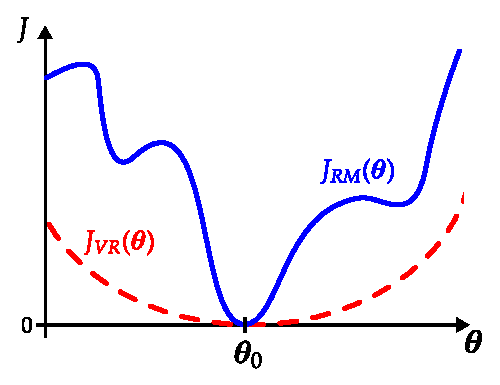
\includegraphics{Figs/JVR_JRM_plot.eps}
   \caption{Typical cost functions for $J_{VR}(\bm{\theta})$ (\usebox0) and $J_{RM}(\bm{\theta})$ (\usebox1).}
   \label{fig:JVR_JRM_plot}
\end{figure}

Note that the Theorem~\ref{thr:theoremVRFT} is valid if the Assumption~\ref{ass:machedControl} is satisfied. In a general case, the structure, or class of $C_0$ is unknown, which ends up leading to the choice of a structure for $C_\theta$ belonging to a class $\mathscr{C}$ such that Assumption~\ref{ass:machedControl} is not satisfied, i.e. $C_0 \notin \mathscr{C} $.
A great contribution of VRFT is the choice of filters that, applied to the sampled signal $\tilde{\bm{u}}$ and the predicted signal $C_\theta[\tilde{\bm{e}}]$, bring the estimated value of $\bm{\theta}$ closer to the optimum value $\bm{\theta}_0$. This subject is discussed in more detail in the Section \ref{sec:filtro_caso_não_linear}.

\section{Controller Parameter Identification}%
\label{sec:controller_parameter_identification}
%TODO: [DONE] {Falar aqui a identificacao dos parametros do controlador, uso de mínimos quadrados, citar o uso de VIs para casos em que a medida é afetada pelo ruído.}

It is considered again that \textit{all} the hypotheses of the Section \ref{sec:vrft_Init_Cons} are satisfied, and that the data acquisition and calculation of virtual values experiment, as described at the beginning of the chapter and illustrated by Figure~\ref{fig:Figs-diagrama_VRFT-eps}, is applied in order to obtain the necessary data. Thus, the vector of parameters that minimizes $J_{VR}(\bm{\theta})$, as \eqref{eq:JVR_reg}, can be estimated by
\begin{equation}
   \bm{\theta} = \left[\sum_{k=1}^{N} \bm{\varphi}(k) \bm{\varphi}(k)^T\right]^{-1} \sum_{k=1}^{N} \bm{\varphi}(k) \tilde{u}(k).
\label{eq:VRFT_LS} 
\end{equation}
Note that \eqref{eq:VRFT_LS} is the same equation presented in \eqref{eq:LS}, however the latter is presented in a matrix form, and the former in the form of a summation.
Therefore, the solution can be written in terms of the ordinary least squares algorithm (OLS) or its derivatives.
Attention is paid to the fact that, in this chapter, the estimated parameter vector $\hat{\bm{\theta}}$ of \eqref{eq:LS} is considered only as $\bm{\theta}$ for reasons of simplification of notation.

When the Assumption \ref{ass:noiseFree} is not satisfied, that is, the sampled is corrupted by noise, the OLS method may not be adequate due to the possible polarization of the estimator parameters caused by these noises \citep{aguirre2015}. 
A common approach used to reduce the effects of this polarization, within the scope of VRFT, is to make use of the instrumental variable estimator, or VI \citep{young1970}. Although, for the purposes of this qualification, noise effects on measurements have not yet been analyzed, and it is assumed that the estimators used are given by OLS estimators.

Another possibility to deal with polarization is to use the extended least squares estimator, or ELS \citep{ljung1999, aguirre2015} in place of OLS, which, as the VI estimator, has the property of reducing polarization (at the cost of an increase in variance). This approach was adopted by \cite{retesNARMAXModelIdentification2019} to structure selection in process model identification with good results. We intend to adapt the metodolgy for controller structure selection and parameter identification in this work. However, it is still in the study phase and will be presented as a future proposal in Chapter \ref{cap:Concl}.


\section{The Unmatched Control and the Filter Selection}%
\label{sec:filtro_caso_não_linear}
As discussed at the end of the Section~\ref{sec:the_ideal_control_design_problem}, if the Assumption ~\ref{ass:machedControl} is not satisfied, i.e. $C_0 \not\in \mathscr{C}$, the Theorem ~\ref{thr:theoremVRFT} no longer applies. Note that this is a recurring situation in practice, since there is, frequently, few information about the process.

However, \cite{campi2006} presents a filter that, when applied to the data used to find the minimizer of $J_{VR}(\bm{\theta})$, produces well-tuned controllers, even when the controller belongs to a class $\mathscr{C}$ other than the $C_0$ class, as long as this class is not ``too far'', that is, the controller should not be too under-parameterized with respect to the control objective.

To achieve the mentioned objective, an increased and filtered cost function is assumed, given by
\begin{equation}
   J_{VR}(\bm{\theta}^{+}) \triangleq \norm{F[C_{\bm{\theta}^{+}}[\tilde{\bm{e}}]] - F[\tilde{\bm{u}}]}^2
\label{eq:JVRplus}
\end{equation}
where $F$ represents the mentioned filter and:
\begin{align}
   \bm{\theta}^+ &\triangleq  [\bm{\theta}^{T} \ \tilde{\theta} ]^T, \quad \tilde{\theta} \in \mathbb{R} ; \\
   C_{\bm{\theta}^+} &\triangleq C_{\theta}+\tilde{\theta}\left(C_0-C_\Delta\right),
\end{align}
where $C_\Delta=C_{\bm{\theta}}$ is computed for $\bm{\theta}=\bm{0}$. It can be verified that:
\begin{itemize}
   \setlength\itemsep{0.1pt}
   \renewcommand{\labelitemi}{--}
   \item $C_0$ é obtido for $\bm{\theta}_0^+ \triangleq [\bm{0}^T\ 1]^T$;
   \item $\left\{C_{\theta}\right\}$ it is obtained by imposing $\tilde{\theta} = 0$.
   \item $C_\Delta$ represents the part of $C_0$ that cannot be explained by the chosen controller family.
\end{itemize}

A new expanded cost function for the reference model is defined as
\begin{align}
   J\left(\bm{\theta}^+\right) &\triangleq \left\|y_{\bm{\theta}^+}-M[\tilde{\bm{r}}]\right\|^2 \\
   \text{ with } y_{\bm{\theta}^+} &=P\left[C_{\theta}+\left[\tilde{\bm{r}}-D y_{\bm{\theta}^+}\right]\right] .
\end{align}

The ideal control objective is to minimize $J_{MR}(\bm{\theta})$, or
\begin{equation}
   \bm{\theta}^+_0 = \argmin_{\theta^+ \in \mathbb{R}^{n_{\theta^+}}}{J_{MR}(\bm{\theta^+})}.
\label{eq:argmqp}
\end{equation}

\cite{campi2006} prove that the objective of minimizing $J_{MR}(\bm{\theta^+}$ can be achieved with good approximation by selecting a filter that guarantees equality between expansions in Taylor series up to the term of degree 2 for $J_{MR}(\bm{\theta^+})$ and $J_{VR}(\bm{\theta}^+)$. By doing this expansion (see Section~\ref{sec:prova_da_escolha_do_filtro_vrft}) it is possible to show that one must have
\begin{equation}
   \left.\frac{\partial^{2} J_{\mathrm{VR}}\left(\bm{\theta}^+\right)}{\partial \bm{\theta}^{+2}}\right|_{\bm{\theta}_{0}^{+}}=\left.\frac{\partial^{2} J\left(\bm{\theta}^+\right)}{\partial \bm{\theta}^{+2}}\right|_{\bm{\theta}_{0}^{+}}.
   \label{eq:condToF}
\end{equation}
% Se esta igualdade é garantida, os mínimos de  e  serão próximos, e consequentemente os parâmetros que os minimizam. Para que isto ocorra, define-se o seguinte teorema:
If this equality is guaranteed, $J_{MR}(\bm{\theta^+})$ and $J_{VR}(\bm{\theta^+})$ will be close each other when they are smaller than one, and consequently the parameters that minimize $J_{VR}(\bm{\theta^+}$, minimize $J_{MR}(\bm{\theta^+}$. For this to happen, the following theorem is defined:
\begin{thm}[\cite{campi2006}] \label{thm:filtro_VRFT_nl}
   If
   \begin{equation}
       F=(I-M D)\left(\left.\frac{\partial P[\bm{u}]}{\partial \bm{u}}\right|_{\tilde{\bm{u}}}\right)
       \label{eq:FilterVRFTNL}
   \end{equation}
   then \eqref{eq:condToF} is satisfied.
\end{thm}

The proof of the Theorem~\ref{thm:filtro_VRFT_nl} is presented in the Section~\ref{sec:prova_da_escolha_do_filtro_vrft} of the Appendix~\ref{cap:AppA}.

A problem presented by the filter \eqref{eq:FilterVRFTNL} is the dependence on the knowledge of a model for the plant. Possible solutions can be obtained using an approximate identified model, which causes the method to lose the characteristic that qualifies it as a DDC system. However, the expression $\left.(\partial P[\bm{u}]/\partial \bm{u})\right|_{\tilde{\bm{u}}}$ is not used for design, only as a filter for the data used in the parametric estimation and an accurate identification is not required.
Furthermore, according to \cite{campi2006}, in many cases, disregarding the derivative of the process and rewriting the filter equation simply as $F=(I-MD)$ results in good results, although there is no guarantee of good approximation.
   
To use the filter, it is sufficient that the sampled signal, $\tilde{\bm{u}}$ and the signal $C_{\bm{\theta}}[\tilde{\bm{e}}]$ are filtered as follows:
\begin{align}
   \tilde{\bm{u}}_f &= F[\tilde{\bm{u}}], \\
   \tilde{C}_f &= F[C_{\bm{\theta}}[\tilde{\bm{e}}]].
\label{eq:}
\end{align}
When the controller is linear in the parameters, we can write
\begin{equation}
   F[C_{\bm{\theta}}[\tilde{\bm{e}}]] = F[\Psi_C \bm{\theta}] = F[\Psi_C]\bm{\theta} \implies \tilde{C}_f = F[\Psi_C] \bm{\theta}.
\end{equation}
From the filtered data ($F[\tilde{\bm{u}}_f]$ and $F[\tilde{C}_f$)], the VRFT procedure is applied in order to minimize the filtered cost function
\begin{equation}
   J_{VR_f}(\bm{\theta}) = \norm{F[\Psi_C] \bm{\theta} - F[\tilde{\bm{u}}]}^2,
\label{eq:JVRfiltrado}
\end{equation}
and the vector parameter that minimizes this cost function can be found by solving
\begin{equation}
   F[\Psi_C]^{T}\left(F[\Psi_C] \bm{\theta}-F[\tilde{\bm{u}}]\right)=0 ,
   % \bm{\theta} = \left(F[\Psi_C]^{T}F[\Psi_C]\right)^{-1}F[\Psi_C]^{T} F[\tilde{\bm{u}}]\right) ,
   \label{eq:OLSFiltered}
\end{equation}
where $\Psi_C$ represents the regressors matrix, a function, in general, of the virtual error $\tilde{\bm{e}}$, the input signal of the process $\tilde{\bm{u}}$ and possibly a vector of residues.
The equation \ref{eq:OLSFiltered} can be solved, for example, by the OLS estimator or by non-polarized estimators for noisy cases. The solution will be the vector  of estimated parameters $\hat{\bm{\theta}}$, that makes the matrix of regressors not correlated with the residual error of the identified controller model ($F[\Psi_C]-F[\tilde{\bm{u}}]$).

\todo[inline]{Falar um pouco sobre o modelo de referência? (uma nova secao) Problema do atraso de transporte e o problema de se exigir mais do que se pode.}

\section{Aplication Examples}%%
\label{sec:aplication_examples}

\begin{exmp}(Controller Parameter identification for a Linear System usinv VRFT procedure)
   \label{exm:31}

   To exemplify the VRFT procedure, a simple case is presented, where the intention is to identify a controller for a second order linear system, according to the VRFT procedure. The adopted model is given by a ``artificial'' system, taken from \cite{wei2008}, and described in the following difference equation, presented as an ARX model:
   \begin{equation}
      y_k = -1.7y_{k-1} -0.8y_{k-2} + u_{k-1} + 0.81u_{k-2} + \eta_k,
   \label{eq:sys_ex_1}
   \end{equation}
   where, $u_{k-i} \in \mathbb{R}$ e $y_{k-i}$ $\in \R$, represent, respectively, the input and output signals for a delay $i$ in respect to $k$; $k$ is the time index; and $\eta_k$ represents the noise in the output signal, which for the purposes of this example, is considered null, i.e. $\eta_k=0$.
   It is considered that the controller must be such that the output of the controlled system follows a reference trajectory imposed by a first order linear system reference model, with the smallest possible error. So, the reference model is choosed 
   So, the reference model is chosen as
   \begin{equation}%
      M(z) = \frac{1-A}{(z-A)z^{d-1}}
   \label{eq:Mz}
   \end{equation}
   where $d$ is the desired pure time delay, $A=e^{-T_s/\tau_M}$ a quantity related to the desired time constant for the closed loop system, given by $\tau_M$, and $T_s$ the sampling time used in the sampling (or decimation) process.
   
   
   From the application of an input signal $\tilde{\bm{u}}=[\tilde{\bm{u}}_1,\ \dots,\ \tilde{\bm{u}}_N]^T$, as a step shape to the process, where $\tilde{\bm{u}} = \bm{u}$ (see \eqref{eq:sys_ex_1}), the response $\tilde{\bm{y}} = [y_1,\ \dots,\ y_N]^T$  is observed. The figure  \ref{fig:u_y_til_VRFT} shows the temporal evolution of these signals (first two top graphs).
   % A partir dos dados colhidos, a referência virtual é  calculada por \eqref{eq:refvirt}
   \begin{figure}[htpb]
      \footnotesize
      \centering
      % \missingfigure{Sinais amostrados}
      % \input{./Matlab/figs/exp31_train_data4.tex}
      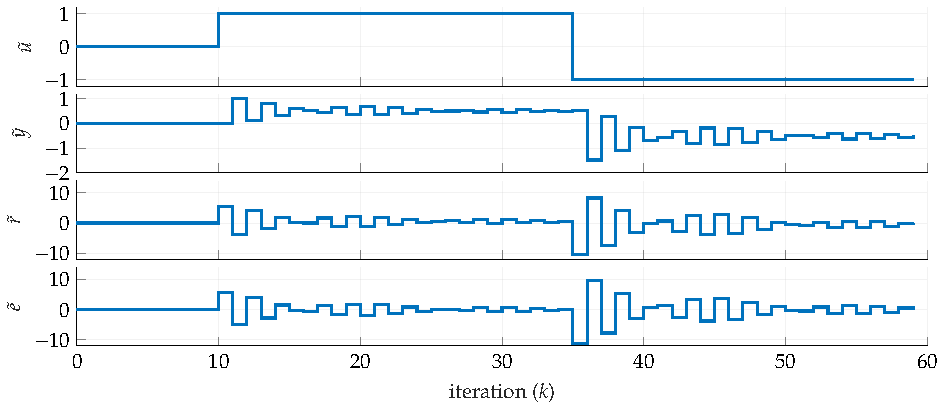
\includegraphics{Figs/exp31_sinais_treinamento.pdf}
      \caption{Temporal evolution of the signals: input of process $\tilde{\bm{u}}$; output of process $\tilde{\bm{y}}$; the calculated virtual reference $\tilde{\bm{r}}$; and the calculated virtual error $\tilde{\bm{e}}$; considering the top to bottom graphs sequence.}
      \label{fig:u_y_til_VRFT}
   \end{figure}
   % \begin{figure}[htpb]
   %    \footnotesize
   %    \centering
   %    % \missingfigure{Sinais amostrados}
   %    % This file was created by matlab2tikz.
%
%The latest updates can be retrieved from
%  http://www.mathworks.com/matlabcentral/fileexchange/22022-matlab2tikz-matlab2tikz
%where you can also make suggestions and rate matlab2tikz.
%
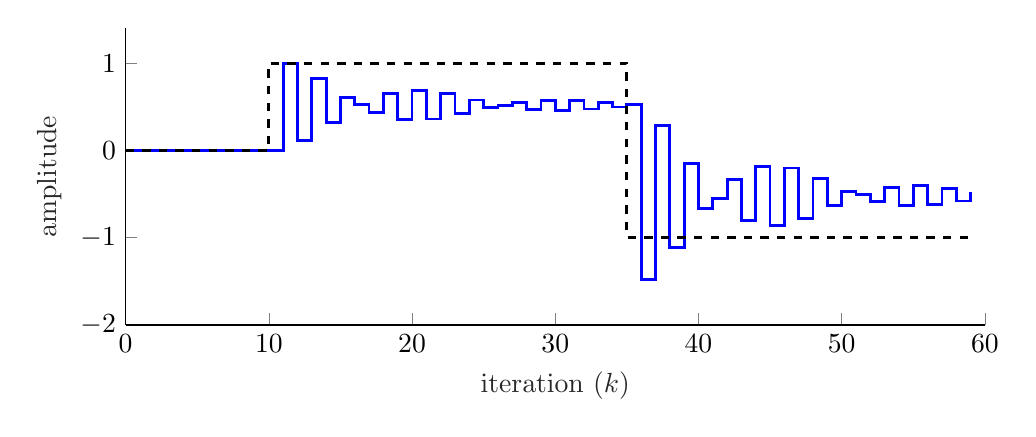
\begin{tikzpicture}

\begin{axis}[%
width=0.9\textwidth,
height=3.769cm,
at={(0\textwidth,0cm)},
scale only axis,
xmin=0,
xmax=60,
xlabel style={font=\color{white!15!black}},
xlabel={iteration ($k$)},
ymin=-2,
ymax=1.4,
ylabel style={font=\color{white!15!black}},
ylabel={amplitude},
axis background/.style={fill=white},
axis x line*=bottom,
axis y line*=left
]
\addplot[const plot, color=blue, line width=1.0pt, forget plot] table[row sep=crcr] {%
0	0\\
11	1\\
12	0.109999999999999\\
13	0.823\\
14	0.322899999999997\\
15	0.602670000000003\\
16	0.527141\\
17	0.431724299999999\\
18	0.654355889999998\\
19	0.352215547\\
20	0.687748858100001\\
21	0.359054503629999\\
22	0.649408257349002\\
23	0.418762359602702\\
24	0.578577382796212\\
25	0.491408561564285\\
26	0.511743539103747\\
27	0.546909134272198\\
28	0.470859640454265\\
29	0.572011303809994\\
30	0.460893071159603\\
31	0.568872735980683\\
32	0.474201891905153\\
33	0.54875859497669\\
34	0.497748875015503\\
35	0.524820036492287\\
36	-1.4803931620493\\
37	0.28681234628997\\
38	-1.11326645905352\\
39	-0.146896896641003\\
40	-0.669662108467485\\
41	-0.554056898292473\\
42	-0.33237358612881\\
43	-0.801719384947049\\
44	-0.18117817668697\\
45	-0.860621591674509\\
46	-0.202000752803755\\
47	-0.778101446894006\\
48	-0.325626938037182\\
49	-0.633953047821585\\
50	-0.471778268273567\\
51	-0.500814505677674\\
52	-0.581192725729103\\
53	-0.421320761718391\\
54	-0.62880052449546\\
55	-0.403982498983012\\
56	-0.620189332132519\\
57	-0.432492136188316\\
58	-0.578611902773851\\
59	-0.4803660563338\\
};
\addplot[const plot, color=black, dashed, line width=1.0pt, forget plot] table[row sep=crcr] {%
0	0\\
10	1\\
35	-1\\
59	-1\\
};
\end{axis}
\end{tikzpicture}%
   %    \caption{Evolução temporal do sinal de excitação $\tilde{\bm{u}}$, e de saída $\tilde{\bm{y}}$, para identificação do controlador pela estratégia VRFT.}
   %    \label{fig:u_y_til_VRFT}
   % \end{figure}
   The process \eqref{eq:sys_ex_1} can be written in the form of a transfer function as
   \begin{equation}
      P(z) = \frac{b_{p 1}z + b_{p 2} }{z^2 + a_{p 1}z + a_{p 2}},
      \label{eq:ex31.Pz}
   \end{equation}
   where $a_{p 1}=1.7$, $a_{p 2}=0.8$, $b_{p 1} = 1$ and $b_{p 2}=0.81$ are the process parameters, given in \eqref{eq:sys_ex_1}.

   Form $\tilde{\bm{y}}$ collected, and the reference model \eqref{eq:Mz}, considering $d=1$,  the virtual  reference could be expressed as \eqref{eq:refvirt}, in the transfer function forma
   \begin{equation}
      \tilde{\bm{r}}_k = M^{-1}(q) \tilde{\bm{y}} = \frac{q-A}{1-A} \tilde{\bm{r}}_k.
   \label{eq:ex31rk}
   \end{equation}
   In \eqref{eq:ex31rk}, $q$ (time shift operator) is adopted instead of $z$ ($z$-transform variable) to emphasize that we are dealing with time responses. This procedure will be adopted throughout this text when needed.

   Note that \eqref{eq:ex31rk} is a non causal system.
   However, since $\tilde{\bm{y}}$ is available in advance, in batch, the calculation can be performed.
   With $\tilde{\bm{r}}$, the virtual error $\tilde{\bm{e}}$ can be easily calculated from \eqref{eq:ev}, as
   \begin{equation*}
      \tilde{\bm{e}}_k = \tilde{\bm{r}}_k - \tilde{\bm{y}}_k 
   \end{equation*}

   Figure \ref{fig:u_y_til_VRFT} shows this \textit{virtual} values (2 bottom ones) calculated over the sampled data $\tilde{\bm{u}}$ and $\tilde{\bm{y}}$ (2 top ones).

   As the process in this example is considered known, the ideal controller $C_0(z)$ can be calculated according to \eqref{eq:Cdz}, replacing \eqref{eq:Mz} and \eqref{eq:ex31.Pz}, i.e.
   \begin{align}
      C_0(z) &= \frac{M(z)}{P(z)\left(1-M(z)\right)} \\
             &= \frac{(1 - A)z^2 + (Aa_{p1} - a_{p1})z - a_{p2} + Aa_{p2}}{b_{p1}z^2 + (b_{p2} - b_{p1})z - b_{p2}} \\
             &= \frac{0.1813 z^2 + 0.3082 z + 0.145}{ z^2 - 0.19 z - 0.81}
   \end{align}
   which can be rewritten in the time domain as:
   \begin{align}
      \label{eq:exp31_uk}
      u_k &= \frac{1 - A}{b_{p1}}e_k + \frac{Aa_{p1} - a_{p1}}{b_{p1}}e_{k-1} + \frac{Aa_{p2} - a_{p2}}{b_{p1}}e_{k-2} - (b_{p2} - b_{p1})u_{k-1} + b_{p2}u_{k-2} \nonumber\\
          &=\begin{bmatrix} e_k & e_{k-1} & e_{k-2} & u_{k-1} & u_{k-2} \end{bmatrix}  \bm{\theta}^\star
   \end{align}
   with ideal parameters given by $\bm{\theta}^\star = [\theta^\star_1 \ \theta^\star_2 \ \theta^\star_3 \ \theta^\star_4 \ \theta^\star_5]^T$. Using the parameters of the process (see \eqref{eq:Mz} and \eqref{eq:sys_ex_1}), a assuming a constant time of $\tau=5$ and a sample time of $T_s=1$, we have $A= 0.8187$ and 
   \begin{equation}
      \bm{\theta}^{\star}= \begin{bmatrix}   0.181 & 0.308 &  0.145 &  0.19 & 0.81 \end{bmatrix}^T.
      \label{eq:exp31_ideal_parameters}
   \end{equation}

   If the ideal parameters are not known, they can be estimated using the sampled data, $\tilde{\bm{u}}$ and $\tilde{\bm{y}}$ instead of $\bm{u}$ and $\bm{y}$ in \eqref{eq:exp31_uk} and, by constructing a matrix of regressors as, for example (it's not the only chice), given by
   \begin{equation*}
      \Psi^T=\begin{bmatrix} \bm{\varphi_1} & \bm{\varphi_1} & \dots & \bm{\varphi_k}  & \dots & \bm{\varphi_N} \end{bmatrix}
   \end{equation*}
   where $\bm{\varphi}^T_k =\begin{bmatrix} \tilde{\bm{e}}_{k} & \tilde{\bm{e}}_{k-1} & \tilde{\bm{e}}_{k-2} & \tilde{\bm{u}}_{k-1} & \tilde{\bm{u}}_{k-2} \end{bmatrix}$ is the vector of regressors.
   Using parameter estimation techniques such as the OLS method, it is possible to estimate $\bm{\theta}$ with good approximation.
   If the excitation signal is persistently exciting, and there is no correlated noise affecting the output, when the number of samples $N$ tends to infinity, i.e. $N \to \infty$, $\bm{\theta}$ tends to $\bm{\theta}^\star$.
   In this example, noise is disregarded and $\bm{\theta}$ is estimated by
   \begin{equation*}
      \hat{\bm{\theta}} = (\Psi^T\Psi)^{-1}\Psi\tilde{\bm{u}}
   \label{eq:}
   \end{equation*}
   
   Performing the procedure described for the data presented, the following cases are considered for controller design:
   \begin{description}
      \item[case A] (Matched Case) A controller in which the vector of regressors $\bm{\varphi}$ has the same structure as the ideal controller is considerr. That is, $\mathscr{C}^{\star} \in \mathscr{C}_A$, where $\mathscr{C}^{\star}$ is the class of the ideal controller and $\mathscr{C}_{A}$, the controller class of the case A;
      \item[case B] (Unmatched Case) It is considered a sub-parameterized controller, with vector of regressors given by $ \bm{\varphi}^T_B =\begin{bmatrix} \tilde{e}_k & \tilde{e}_{k-1} & \tilde{e}_{k-2} & \tilde{u}_{k-1} \end{bmatrix}$, i.e. $\mathscr{C}^\star \not\in \mathscr{C}_B $;
      \item[case C] (PID Unmatched Case) It is considered a sub-parameterized controller with a vector of regressors built according to the structure of a PID controller, defined as
         \begin{align}
            C_{C}(q) &= \left(K_p + K_i\frac{q}{q-1} + K_d\frac{q-1}{q}\right)\tilde{\bm{e}}_k \nonumber \\
                     &= \left(K_p + K_i\frac{q}{q-1} + K_d\frac{q-1}{q}\right)\left(\tilde{\bm{r}}_k-\tilde{\bm{y}}_k\right) \nonumber \\
                     &= \left(K_p + K_i\frac{q}{q-1} + K_d\frac{q-1}{q}\right)\left(\frac{q-A}{1-A}-1\right)\tilde{\bm{y}}_k \nonumber \\
                     &= \left(K_p + K_i\frac{q}{q-1} + K_d\frac{q-1}{q}\right)\frac{q-1}{1-A}\tilde{\bm{y}} \nonumber \\
                     &= \begin{bmatrix} 
                        \dfrac{\tilde{\bm{y}}_{k+1}-\tilde{\bm{y}}_k}{1-a} & 
                        \dfrac{\tilde{\bm{y}}_{k+1}}{1-a} &
                        \dfrac{\tilde{\bm{y}}_{k+1}-2*\tilde{\bm{y}}_k+\tilde{\bm{y}}_{k-1}}{1-a} 
                     \end{bmatrix} 
            \begin{bmatrix}  K_p & K_i & K_d  \end{bmatrix}^T   
            \label{eq:} 
         \end{align}
% COMTEMP          \todo{Colocar detalhes do processo de construcao do regressor no apêndice?}
         The vector of regressors, in this case, is described by
         \begin{equation}
            \bm{\varphi}^T_C = \begin{bmatrix} 
               (\tilde{\bm{y}}_{k+1}-\tilde{\bm{y}}_k)/(1-a) &
               (\tilde{\bm{y}}_{k+1})/(1-a) &
               (\tilde{\bm{y}}_{k+1}-2*\tilde{\bm{y}}_k+\tilde{\bm{y}}_{k-1})/(1-a)
            \end{bmatrix} 
            \label{eq:}
         \end{equation}
   \end{description}
   Note that, although the regressor in case B has fewer terms than the regressor in case A, the controller belongs to the class of controller A, since it can be written by
   \begin{equation*}
      C_C(z) = \frac{(Kd + Ki + Kp)z^2 + (- 2Kd - Kp)z + Kd}{z^2 - z}
   \end{equation*}
   however, the controller class in case A is broader (class B is contained in class A).
   By the same procedure of identification described earlier, the following parameters are obtained for the 3 cases:
   \begin{align}
      \label{eq:ex31_par3casos}
      \bm{\theta}_A^T &= \begin{bmatrix}   0.181 & 0.308 &  0.145 &  0.19 & 0.81 \end{bmatrix} = \bm{\theta}^\star \nonumber \\
      \bm{\theta}_B^T &= \begin{bmatrix}   0.168 & 0.166 & 0.039 & 0.988 \end{bmatrix} \nonumber \\
      \bm{\theta}_C^T &= \begin{bmatrix}   -0.202 & 0.351 & 0.0229 \end{bmatrix} \nonumber 
   \end{align}
   
   Figure~\ref{fig:exp31_time_resp} shows the temporal response of the closed-loop system with the controllers obtained for the 3 cases, together with the signal from the reference model. It is considered a square reference signal and that a disturbance of magnitude 0.5 is applied at the output, at time $k=75$. The figure also shows the answer for a fourth case to be discussed ahead.
   \begin{figure}[htpb]
      \sbox0{\blackdottedline} \sbox1{\redsolidline} \sbox2{\bluedashedline} \sbox3{\greendashdottedline} \sbox4{\magentadottedline}
      \footnotesize
      \centering
      \hspace*{-1cm}
      % \input{./Matlab/figs/exp31_time_response.tex}
      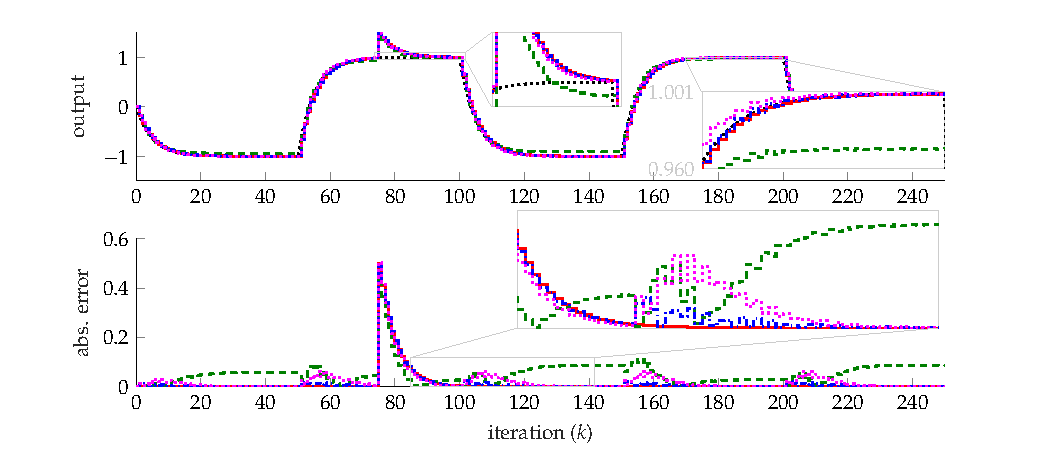
\includegraphics{Figs/ex31_resptemporal.pdf}
      \caption{Closed-loop system response to a square reference signal (upper graph) and absolute error (lower graph) for: case A (\usebox1); case B (\usebox2); case C (\usebox3); and case D (\usebox4). The response of the reference model is represented by (\usebox0) in the upper graph.}
      \label{fig:exp31_time_resp}
   \end{figure}
   % ticklabel style = {font=\scriptsize},
   % y tick label style={/pgf/number format/.cd,%
   %           scaled y ticks = false,
   %           precision = 3,
   %           fixed,
   %           fixed zerofill
   %         },

   Note that in Case A, because it has the same structure and parameters as the ideal controller, it has an identical response to the reference model (except, obviously, at the transient period after the application of the disturbance).
   %
   Differently, Case B presents some tracking error, even on steady state. This can be explained by the fact that the controller model was not able to reproduce an integration effect. This effect can be observed when the sum of the coefficients of the terms in $\tilde{\bm{u}}$ that make up the regressor, results in 1. In this case, the coefficient of $\tilde{\bm{u}}_{k-1}$ (only regressor in $\tilde{\bm{u}}$) is $0.988 \approx 1$, but not exactly 1.
   %
   Case 3, due to the way in which the regressor is built, a restriction is imposed on the controller structure in such a way that an integrator effect is forced, which allows the controller to be expressed with only 3 regressors. The result, as can be seen in Figure~\ref{fig:exp31_time_resp}, is the elimination of tracking error in steady state, even under the effect of external disturbance.
%
   It is emphasized here that, although the integration effect is not present in case B, this can be imposed, for example, with the use of methods such as \textit{Restricted Least Squares}, or CLS~\citep{draper1998}. Case D presented below considers this modification applied in case B, restricting the coefficient of $\tilde{\bm{u}}_{k-1}$ to be equals one and imposing an integrator in controller. The time response is also shown in Figure \ref{fig:exp31_time_resp}.

   \begin{description}
   \item[case D] In this case, it is considered that the CLS procedure is adopted after the parameter estimation in case B. The $c=S \bm{\theta}_B$ restriction is assumed, with $c=1$ and $S = [0\ 0\ 0 \ 1]^T$. The new parameter vector $\bm{\theta}_D$ is calculated by \citep{draper1998}:
         \begin{equation}
            \bm{\theta}_D = (\Psi^T\Psi)^{-1}\tilde{\bm{y}} - (\Psi^T\Psi)^{-1}S^T\left[(\Psi^T\Psi)^{-1}S^T\right]^{-1}\left(S\bm{\theta}_{B} - c\right)
         \end{equation}
   where $\Psi^T = \begin{bmatrix} \bm{\varphi}_{B}(1) & \bm{\varphi}_{B}(2) & \dots & \bm{\varphi}_{B}(N) \end{bmatrix} $ represents the regressor matrix, and $\bm{\varphi}_B(k) = \begin{bmatrix} \tilde{e}_k & \tilde{e}_{k-1} & \tilde{e}_{k-2} & \tilde{u}_{k-1} \end{bmatrix}^T$, with $k=1,\dots,N$, is the vector of regressors at instant $k$.
   \end{description}

   As can be seen in Figure~\ref{fig:exp31_time_resp}, the error in steady state is eliminated, as expected.

\end{exmp}

\subsection{ Final Considerations of the Chapter }%
\label{sub:considerações_finais}

A benefit of specifying the controller as in case C of the Example~\ref{exm:31}, is that it starts from a priori knowledge (i.e., it is known that the controller must have an integrator). For many cases, where is desired to tune a pre-existing controller, such as controllers in the PID family, this can be very useful. This fact has great appeal in industrial applications.

However, there are cases where a precise control is needed. Especially for strongly non-linear systems, where a controller with an adequate pre-established structure (which may be non-linear) can be difficult to obtain.
In this sense, the main focus of this work is on the selection of this appropriate structure with no (or some) prior knowledge. Only from sampled data. As will be seen later, in Chapter \ref{cap:CCS}, a method for searching the appropriate controller structure by a randomized approach is proposed.
possa
In this case, it will be necessary to easily generate a sufficiently large universe of models.
For this purpose, representing these controllers using polinomial structures like NBRX (or NBRMBX) models, generically, as done in case B of Example~\ref{exm:31}, instead of predefined structures as done in case C, is an advantage.
In order to take advantage of known or desired information about the controller, a proposal of this work is to include this information in the  identification process in a posteriori way, using, for example, the CLS estimator, as shown in case D of the example.

As will be seen, the VRFT method will be one of the main tools used for the framework proposed in chapter \ref{cap:CCS}.

% \begin{figure}[H]
%    \centering
%    % % This file was created by matlab2tikz.
%
%The latest updates can be retrieved from
%  http://www.mathworks.com/matlabcentral/fileexchange/22022-matlab2tikz-matlab2tikz
%where you can also make suggestions and rate matlab2tikz.
%
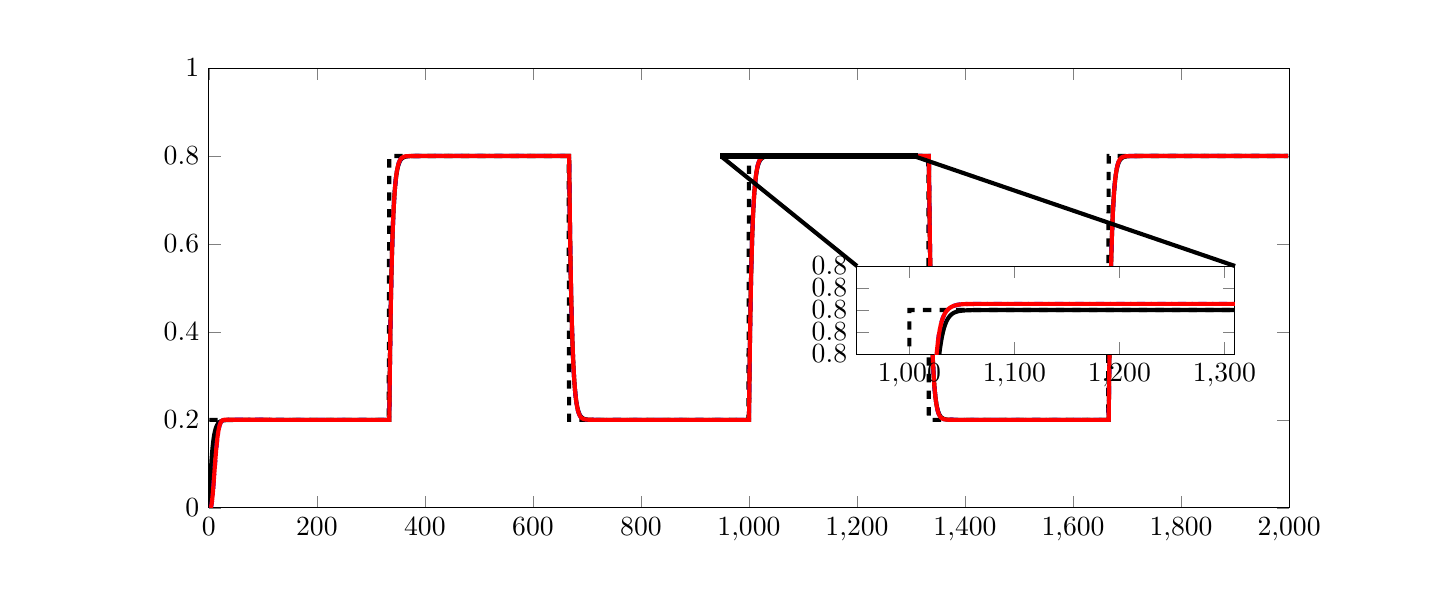
\begin{tikzpicture}

\begin{axis}[%
width=5.401in,
height=2.199in,
at={(0.906in,0.297in)},
scale only axis,
xmin=0,
xmax=2000,
ymin=0,
ymax=1,
axis background/.style={fill=white}
]
\addplot [color=black, dashed, line width=1.5pt, forget plot]
  table[row sep=crcr]{%
1	0.200000000000045\\
333	0.200000000000045\\
334	0.799999999999955\\
666	0.799999999999955\\
667	0.200000000000045\\
999	0.200000000000045\\
1000	0.799999999999955\\
1332	0.799999999999955\\
1333	0.200000000000045\\
1665	0.200000000000045\\
1666	0.799999999999955\\
1998	0.799999999999955\\
};
\addplot [color=black, line width=1.5pt, forget plot]
  table[row sep=crcr]{%
1	0\\
2	0.0362538493843658\\
3	0.0659359907929229\\
4	0.0902376727810861\\
5	0.110134207176543\\
6	0.1264241117658\\
7	0.139761157617613\\
8	0.150680607211598\\
9	0.159620696401134\\
10	0.166940222355606\\
11	0.172932943352635\\
12	0.177839368327568\\
13	0.181856409342117\\
15	0.18783798747495\\
17	0.191847559204234\\
19	0.194535255510573\\
22	0.197000884635827\\
26	0.198652410600289\\
32	0.199594113872763\\
45	0.199969853385028\\
163	0.200000000000045\\
334	0.200000000000045\\
335	0.308761548153143\\
336	0.397807972378587\\
337	0.470713018343531\\
338	0.530402621529674\\
339	0.579272335297219\\
340	0.619283472852658\\
341	0.652041821635066\\
342	0.678862089203221\\
343	0.700820667067092\\
344	0.718798830057949\\
345	0.733518104982522\\
346	0.745569228026397\\
347	0.755435853071504\\
348	0.763513962424895\\
349	0.770127758979243\\
350	0.775542677612975\\
351	0.779976038023733\\
352	0.783605766531537\\
354	0.789010616666701\\
356	0.792633596058067\\
358	0.79506215177048\\
361	0.797290051434402\\
365	0.798782341618335\\
371	0.799633248343298\\
385	0.799977697808799\\
543	0.799999999999955\\
667	0.799999999999955\\
668	0.691238451846857\\
669	0.602192027621413\\
670	0.529286981656469\\
671	0.469597378470326\\
672	0.420727664702781\\
673	0.380716527147342\\
674	0.347958178364934\\
675	0.321137910796779\\
676	0.299179332932908\\
677	0.281201169942051\\
678	0.266481895017478\\
679	0.254430771973603\\
680	0.244564146928496\\
681	0.236486037575105\\
682	0.229872241020757\\
683	0.224457322387025\\
684	0.220023961976267\\
685	0.216394233468463\\
687	0.210989383333299\\
689	0.207366403941933\\
691	0.20493784822952\\
694	0.202709948565598\\
698	0.201217658381665\\
704	0.200366751656702\\
718	0.200022302191201\\
876	0.200000000000045\\
1000	0.200000000000045\\
1001	0.308761548153143\\
1002	0.397807972378587\\
1003	0.470713018343531\\
1004	0.530402621529674\\
1005	0.579272335297219\\
1006	0.619283472852658\\
1007	0.652041821635066\\
1008	0.678862089203221\\
1009	0.700820667067092\\
1010	0.718798830057949\\
1011	0.733518104982522\\
1012	0.745569228026397\\
1013	0.755435853071504\\
1014	0.763513962424895\\
1015	0.770127758979243\\
1016	0.775542677612975\\
1017	0.779976038023733\\
1018	0.783605766531537\\
1020	0.789010616666701\\
1022	0.792633596058067\\
1024	0.79506215177048\\
1027	0.797290051434402\\
1031	0.798782341618335\\
1037	0.799633248343298\\
1051	0.799977697808799\\
1209	0.799999999999955\\
1333	0.799999999999955\\
1334	0.691238451846857\\
1335	0.602192027621413\\
1336	0.529286981656469\\
1337	0.469597378470326\\
1338	0.420727664702781\\
1339	0.380716527147342\\
1340	0.347958178364934\\
1341	0.321137910796779\\
1342	0.299179332932908\\
1343	0.281201169942051\\
1344	0.266481895017478\\
1345	0.254430771973603\\
1346	0.244564146928496\\
1347	0.236486037575105\\
1348	0.229872241020757\\
1349	0.224457322387025\\
1350	0.220023961976267\\
1351	0.216394233468463\\
1353	0.210989383333299\\
1355	0.207366403941933\\
1357	0.20493784822952\\
1360	0.202709948565598\\
1364	0.201217658381665\\
1370	0.200366751656702\\
1384	0.200022302191201\\
1542	0.200000000000045\\
1666	0.200000000000045\\
1667	0.308761548153143\\
1668	0.397807972378587\\
1669	0.470713018343531\\
1670	0.530402621529674\\
1671	0.579272335297219\\
1672	0.619283472852658\\
1673	0.652041821635066\\
1674	0.678862089203221\\
1675	0.700820667067092\\
1676	0.718798830057949\\
1677	0.733518104982522\\
1678	0.745569228026397\\
1679	0.755435853071504\\
1680	0.763513962424895\\
1681	0.770127758979243\\
1682	0.775542677612975\\
1683	0.779976038023733\\
1684	0.783605766531537\\
1686	0.789010616666701\\
1688	0.792633596058067\\
1690	0.79506215177048\\
1693	0.797290051434402\\
1697	0.798782341618335\\
1703	0.799633248343298\\
1717	0.799977697808799\\
1875	0.799999999999955\\
1998	0.799999999999955\\
};
\addplot [color=blue, dashdotted, line width=1.5pt, forget plot]
  table[row sep=crcr]{%
1	0\\
3	0\\
4	0.0022944138117964\\
5	0.00802600781457841\\
6	0.0172228809271928\\
7	0.0295123170046736\\
8	0.0441062415504803\\
9	0.0602118445510769\\
11	0.0937054630521743\\
12	0.10978717548619\\
13	0.12479726870788\\
14	0.138422065150507\\
15	0.150501853993319\\
16	0.160964178216091\\
17	0.169838276715382\\
18	0.177203407527713\\
19	0.183192186933184\\
20	0.187954374246146\\
21	0.19165768503558\\
22	0.194464801601498\\
24	0.198010802310137\\
26	0.199676340225096\\
29	0.200348647311557\\
188	0.200070171134257\\
334	0.200070171134257\\
335	0.305609229915945\\
336	0.399046898273355\\
337	0.468452131562117\\
338	0.530232657723445\\
339	0.576663738976777\\
340	0.618116024785877\\
341	0.649606084789184\\
342	0.677709357983076\\
343	0.699234039863768\\
344	0.718371511510441\\
345	0.733098336172816\\
346	0.746104694457244\\
347	0.756123617763478\\
348	0.76489461405663\\
349	0.771634868230876\\
350	0.777476724517101\\
351	0.781942637136353\\
352	0.785773245494738\\
354	0.791148958394388\\
356	0.7945701424444\\
358	0.796711727627098\\
361	0.798477987589422\\
365	0.799516622560532\\
373	0.800113739859853\\
399	0.800280176832302\\
667	0.800280684537483\\
668	0.694741625756023\\
669	0.601303957398613\\
670	0.531898724109624\\
671	0.470118197948295\\
672	0.423687116695191\\
673	0.382234830886091\\
674	0.350744770882557\\
675	0.322641497688664\\
676	0.301116815807973\\
677	0.2819793441613\\
678	0.267252519499152\\
679	0.254246161214496\\
680	0.24422723790849\\
681	0.235456241615111\\
682	0.228715987441092\\
683	0.22287413115464\\
684	0.218408218535387\\
685	0.214577610177002\\
687	0.209201897277353\\
689	0.205780713227341\\
691	0.203639128044642\\
694	0.201872868082319\\
698	0.200834233111436\\
706	0.200237115811888\\
732	0.200070678839438\\
1000	0.200070171134257\\
1001	0.305609229915945\\
1002	0.399046898273355\\
1003	0.468452131562117\\
1004	0.530232657723445\\
1005	0.576663738976777\\
1006	0.618116024785877\\
1007	0.649606084789184\\
1008	0.677709357983076\\
1009	0.699234039863768\\
1010	0.718371511510441\\
1011	0.733098336172816\\
1012	0.746104694457244\\
1013	0.756123617763478\\
1014	0.76489461405663\\
1015	0.771634868230876\\
1016	0.777476724517101\\
1017	0.781942637136353\\
1018	0.785773245494738\\
1020	0.791148958394388\\
1022	0.7945701424444\\
1024	0.796711727627098\\
1027	0.798477987589422\\
1031	0.799516622560532\\
1039	0.800113739859853\\
1065	0.800280176832302\\
1333	0.800280684537483\\
1334	0.694741625756023\\
1335	0.601303957398613\\
1336	0.531898724109624\\
1337	0.470118197948295\\
1338	0.423687116695191\\
1339	0.382234830886091\\
1340	0.350744770882557\\
1341	0.322641497688664\\
1342	0.301116815807973\\
1343	0.2819793441613\\
1344	0.267252519499152\\
1345	0.254246161214496\\
1346	0.24422723790849\\
1347	0.235456241615111\\
1348	0.228715987441092\\
1349	0.22287413115464\\
1350	0.218408218535387\\
1351	0.214577610177002\\
1353	0.209201897277353\\
1355	0.205780713227341\\
1357	0.203639128044642\\
1360	0.201872868082319\\
1364	0.200834233111436\\
1372	0.200237115811888\\
1398	0.200070678839438\\
1666	0.200070171134257\\
1667	0.305609229915945\\
1668	0.399046898273355\\
1669	0.468452131562117\\
1670	0.530232657723445\\
1671	0.576663738976777\\
1672	0.618116024785877\\
1673	0.649606084789184\\
1674	0.677709357983076\\
1675	0.699234039863768\\
1676	0.718371511510441\\
1677	0.733098336172816\\
1678	0.746104694457244\\
1679	0.756123617763478\\
1680	0.76489461405663\\
1681	0.771634868230876\\
1682	0.777476724517101\\
1683	0.781942637136353\\
1684	0.785773245494738\\
1686	0.791148958394388\\
1688	0.7945701424444\\
1690	0.796711727627098\\
1693	0.798477987589422\\
1697	0.799516622560532\\
1705	0.800113739859853\\
1731	0.800280176832302\\
1998	0.800280684537483\\
};
\addplot [color=red, line width=1.5pt, forget plot]
  table[row sep=crcr]{%
1	0\\
3	0\\
4	0.0022944138117964\\
5	0.00802600781457841\\
6	0.0172228809271928\\
7	0.0295123170046736\\
8	0.0441062415504803\\
9	0.0602118445510769\\
11	0.0937054630521743\\
12	0.10978717548619\\
13	0.12479726870788\\
14	0.138422065150507\\
15	0.150501853993319\\
16	0.160964178216091\\
17	0.169838276715382\\
18	0.177203407527713\\
19	0.183192186933184\\
20	0.187954374246146\\
21	0.19165768503558\\
22	0.194464801601498\\
24	0.198010802310137\\
26	0.199676340225096\\
29	0.200348647311557\\
188	0.200070171134257\\
334	0.200070171134257\\
335	0.305609229915945\\
336	0.399046898273355\\
337	0.468452131562117\\
338	0.530232657723445\\
339	0.576663738976777\\
340	0.618116024785877\\
341	0.649606084789184\\
342	0.677709357983076\\
343	0.699234039863768\\
344	0.718371511510441\\
345	0.733098336172816\\
346	0.746104694457244\\
347	0.756123617763478\\
348	0.76489461405663\\
349	0.771634868230876\\
350	0.777476724517101\\
351	0.781942637136353\\
352	0.785773245494738\\
354	0.791148958394388\\
356	0.7945701424444\\
358	0.796711727627098\\
361	0.798477987589422\\
365	0.799516622560532\\
373	0.800113739859853\\
399	0.800280176832302\\
667	0.800280684537483\\
668	0.694741625756023\\
669	0.601303957398613\\
670	0.531898724109624\\
671	0.470118197948295\\
672	0.423687116695191\\
673	0.382234830886091\\
674	0.350744770882557\\
675	0.322641497688664\\
676	0.301116815807973\\
677	0.2819793441613\\
678	0.267252519499152\\
679	0.254246161214496\\
680	0.24422723790849\\
681	0.235456241615111\\
682	0.228715987441092\\
683	0.22287413115464\\
684	0.218408218535387\\
685	0.214577610177002\\
687	0.209201897277353\\
689	0.205780713227341\\
691	0.203639128044642\\
694	0.201872868082319\\
698	0.200834233111436\\
706	0.200237115811888\\
732	0.200070678839438\\
1000	0.200070171134257\\
1001	0.305609229915945\\
1002	0.399046898273355\\
1003	0.468452131562117\\
1004	0.530232657723445\\
1005	0.576663738976777\\
1006	0.618116024785877\\
1007	0.649606084789184\\
1008	0.677709357983076\\
1009	0.699234039863768\\
1010	0.718371511510441\\
1011	0.733098336172816\\
1012	0.746104694457244\\
1013	0.756123617763478\\
1014	0.76489461405663\\
1015	0.771634868230876\\
1016	0.777476724517101\\
1017	0.781942637136353\\
1018	0.785773245494738\\
1020	0.791148958394388\\
1022	0.7945701424444\\
1024	0.796711727627098\\
1027	0.798477987589422\\
1031	0.799516622560532\\
1039	0.800113739859853\\
1065	0.800280176832302\\
1333	0.800280684537483\\
1334	0.694741625756023\\
1335	0.601303957398613\\
1336	0.531898724109624\\
1337	0.470118197948295\\
1338	0.423687116695191\\
1339	0.382234830886091\\
1340	0.350744770882557\\
1341	0.322641497688664\\
1342	0.301116815807973\\
1343	0.2819793441613\\
1344	0.267252519499152\\
1345	0.254246161214496\\
1346	0.24422723790849\\
1347	0.235456241615111\\
1348	0.228715987441092\\
1349	0.22287413115464\\
1350	0.218408218535387\\
1351	0.214577610177002\\
1353	0.209201897277353\\
1355	0.205780713227341\\
1357	0.203639128044642\\
1360	0.201872868082319\\
1364	0.200834233111436\\
1372	0.200237115811888\\
1398	0.200070678839438\\
1666	0.200070171134257\\
1667	0.305609229915945\\
1668	0.399046898273355\\
1669	0.468452131562117\\
1670	0.530232657723445\\
1671	0.576663738976777\\
1672	0.618116024785877\\
1673	0.649606084789184\\
1674	0.677709357983076\\
1675	0.699234039863768\\
1676	0.718371511510441\\
1677	0.733098336172816\\
1678	0.746104694457244\\
1679	0.756123617763478\\
1680	0.76489461405663\\
1681	0.771634868230876\\
1682	0.777476724517101\\
1683	0.781942637136353\\
1684	0.785773245494738\\
1686	0.791148958394388\\
1688	0.7945701424444\\
1690	0.796711727627098\\
1693	0.798477987589422\\
1697	0.799516622560532\\
1705	0.800113739859853\\
1731	0.800280176832302\\
1998	0.800280684537483\\
};
\end{axis}

\begin{axis}[%
width=1.89in,
height=0.44in,
at={(4.146in,1.066in)},
scale only axis,
xmin=950,
xmax=1310,
ymin=0.798,
ymax=0.802,
axis background/.style={fill=white}
]
\addplot [color=black, dashed, line width=1.5pt, forget plot]
  table[row sep=crcr]{%
999.996	0.797600000000102\\
1000	0.799999999999955\\
1311	0.799999999999955\\
};
\addplot [color=black, line width=1.5pt, forget plot]
  table[row sep=crcr]{%
1028	0.797781281770085\\
1029	0.798183467152739\\
1030	0.798512748694066\\
1031	0.798782341618335\\
1032	0.799003065636043\\
1033	0.799183779177383\\
1034	0.79933173491122\\
1035	0.799452870820687\\
1036	0.799552048514897\\
1037	0.799633248343298\\
1038	0.799699729140002\\
1039	0.799754159012537\\
1040	0.799798722423247\\
1041	0.799835207857996\\
1042	0.799865079605524\\
1043	0.799889536523779\\
1044	0.799909560154902\\
1045	0.799925954117498\\
1047	0.799950365560562\\
1049	0.799966729040307\\
1051	0.799977697808799\\
1054	0.799987760297881\\
1058	0.799994500347339\\
1064	0.799998343536345\\
1077	0.799999876968513\\
1193	0.799999999999955\\
1311	0.799999999999955\\
};
\addplot [color=blue, dashdotted, line width=1.5pt, forget plot]
  table[row sep=crcr]{%
1025.27687493329	0.797600000000102\\
1026	0.798035179212093\\
1027	0.798477987589422\\
1028	0.798847724656071\\
1029	0.799119507913701\\
1030	0.799347890408626\\
1031	0.799516622560532\\
1032	0.799660005570558\\
1033	0.799767189221711\\
1034	0.799859568301827\\
1035	0.799929806031741\\
1036	0.799991182391977\\
1037	0.80003873091664\\
1038	0.800080692994015\\
1039	0.800113739859853\\
1040	0.800143014406331\\
1041	0.800166328117712\\
1042	0.800186927212735\\
1044	0.800217861523606\\
1046	0.800239420781963\\
1048	0.800254168730817\\
1050	0.800264016930214\\
1053	0.80027263529837\\
1057	0.800277747192695\\
1064	0.800280076547324\\
1094	0.800280683756455\\
1311	0.800280684537483\\
};
\addplot [color=red, line width=1.5pt, forget plot]
  table[row sep=crcr]{%
1025.27687493329	0.797600000000102\\
1026	0.798035179212093\\
1027	0.798477987589422\\
1028	0.798847724656071\\
1029	0.799119507913701\\
1030	0.799347890408626\\
1031	0.799516622560532\\
1032	0.799660005570558\\
1033	0.799767189221711\\
1034	0.799859568301827\\
1035	0.799929806031741\\
1036	0.799991182391977\\
1037	0.80003873091664\\
1038	0.800080692994015\\
1039	0.800113739859853\\
1040	0.800143014406331\\
1041	0.800166328117712\\
1042	0.800186927212735\\
1044	0.800217861523606\\
1046	0.800239420781963\\
1048	0.800254168730817\\
1050	0.800264016930214\\
1053	0.80027263529837\\
1057	0.800277747192695\\
1064	0.800280076547324\\
1094	0.800280683756455\\
1311	0.800280684537483\\
};
\end{axis}

\begin{axis}[%
width=6.969in,
height=2.698in,
at={(0in,0in)},
scale only axis,
xmin=0,
xmax=1,
ymin=0,
ymax=1,
axis line style={draw=none},
ticks=none,
axis x line*=bottom,
axis y line*=left
]
\draw[line width=1.5pt, draw=black] (axis cs:0.498125,0.76037) rectangle (axis cs:0.637625,0.76363);
\addplot [color=black, line width=1.5pt, forget plot]
  table[row sep=crcr]{%
0.498125	0.76037\\
0.595	0.55825\\
};
\addplot [color=black, line width=1.5pt, forget plot]
  table[row sep=crcr]{%
0.637625	0.76037\\
0.86625	0.55825\\
};
\end{axis}
\end{tikzpicture}%
%    % % Created by tikzDevice version 0.12.3.1 on 2021-04-22 16:14:12
% !TEX encoding = UTF-8 Unicode
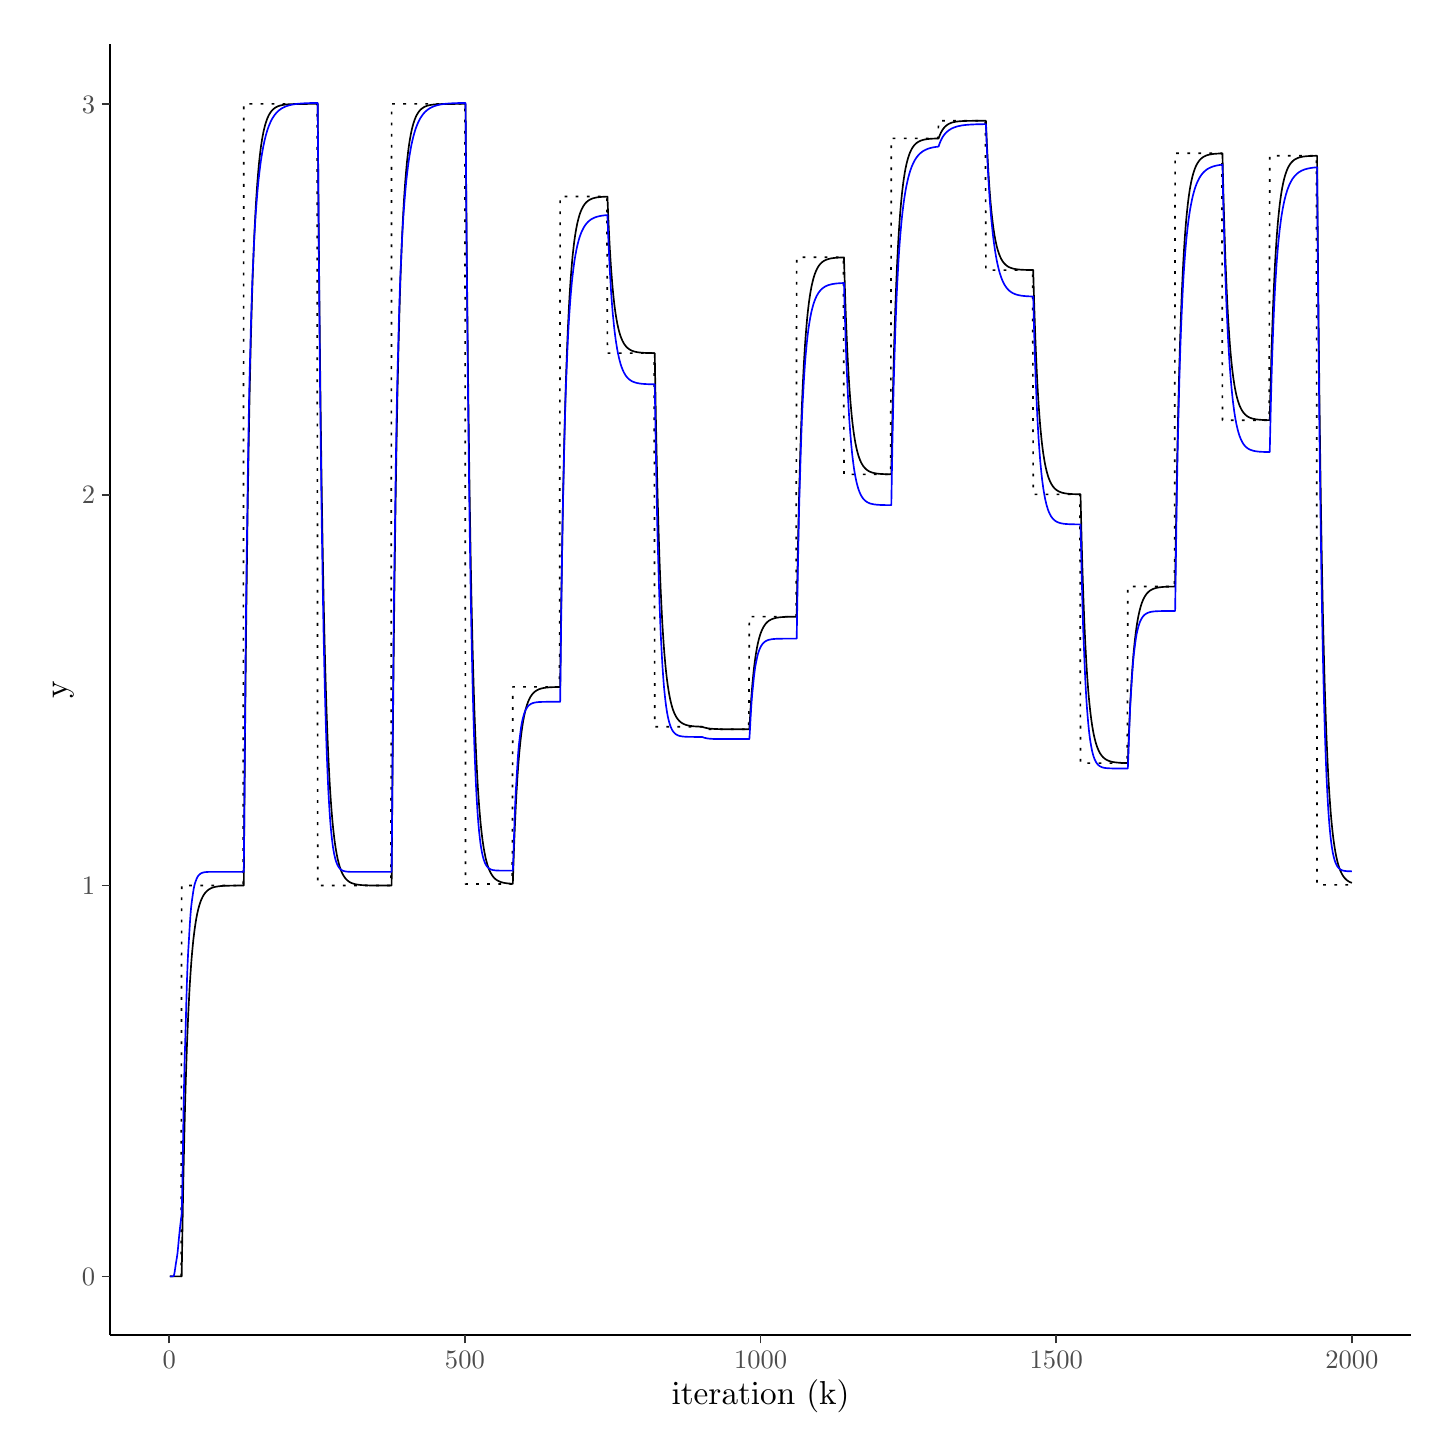
\begin{tikzpicture}[x=1pt,y=1pt]
\definecolor{fillColor}{RGB}{255,255,255}
\path[use as bounding box,fill=fillColor,fill opacity=0.00] (0,0) rectangle (505.89,505.89);
\begin{scope}
\path[clip] (  0.00,  0.00) rectangle (505.89,505.89);
\definecolor{drawColor}{RGB}{255,255,255}
\definecolor{fillColor}{RGB}{255,255,255}

\path[draw=drawColor,line width= 0.6pt,line join=round,line cap=round,fill=fillColor] (  0.00,  0.00) rectangle (505.89,505.89);
\end{scope}
\begin{scope}
\path[clip] ( 29.80, 33.48) rectangle (499.89,499.89);
\definecolor{fillColor}{RGB}{255,255,255}

\path[fill=fillColor] ( 29.80, 33.48) rectangle (499.89,499.89);
\definecolor{drawColor}{RGB}{0,0,0}

\path[draw=drawColor,line width= 0.6pt,dash pattern=on 1pt off 3pt ,line join=round] ( 51.38, 54.68) --
	( 51.59, 54.68) --
	( 51.81, 54.68) --
	( 52.02, 54.68) --
	( 52.23, 54.68) --
	( 52.45, 54.68) --
	( 52.66, 54.68) --
	( 52.87, 54.68) --
	( 53.09, 54.68) --
	( 53.30, 54.68) --
	( 53.51, 54.68) --
	( 53.73, 54.68) --
	( 53.94, 54.68) --
	( 54.16, 54.68) --
	( 54.37, 54.68) --
	( 54.58, 54.68) --
	( 54.80, 54.68) --
	( 55.01, 54.68) --
	( 55.22, 54.68) --
	( 55.44, 54.68) --
	( 55.65,195.90) --
	( 55.87,195.90) --
	( 56.08,195.90) --
	( 56.29,195.90) --
	( 56.51,195.90) --
	( 56.72,195.90) --
	( 56.93,195.90) --
	( 57.15,195.90) --
	( 57.36,195.90) --
	( 57.57,195.90) --
	( 57.79,195.90) --
	( 58.00,195.90) --
	( 58.22,195.90) --
	( 58.43,195.90) --
	( 58.64,195.90) --
	( 58.86,195.90) --
	( 59.07,195.90) --
	( 59.28,195.90) --
	( 59.50,195.90) --
	( 59.71,195.90) --
	( 59.92,195.90) --
	( 60.14,195.90) --
	( 60.35,195.90) --
	( 60.57,195.90) --
	( 60.78,195.90) --
	( 60.99,195.90) --
	( 61.21,195.90) --
	( 61.42,195.90) --
	( 61.63,195.90) --
	( 61.85,195.90) --
	( 62.06,195.90) --
	( 62.28,195.90) --
	( 62.49,195.90) --
	( 62.70,195.90) --
	( 62.92,195.90) --
	( 63.13,195.90) --
	( 63.34,195.90) --
	( 63.56,195.90) --
	( 63.77,195.90) --
	( 63.98,195.90) --
	( 64.20,195.90) --
	( 64.41,195.90) --
	( 64.63,195.90) --
	( 64.84,195.90) --
	( 65.05,195.90) --
	( 65.27,195.90) --
	( 65.48,195.90) --
	( 65.69,195.90) --
	( 65.91,195.90) --
	( 66.12,195.90) --
	( 66.34,195.90) --
	( 66.55,195.90) --
	( 66.76,195.90) --
	( 66.98,195.90) --
	( 67.19,195.90) --
	( 67.40,195.90) --
	( 67.62,195.90) --
	( 67.83,195.90) --
	( 68.04,195.90) --
	( 68.26,195.90) --
	( 68.47,195.90) --
	( 68.69,195.90) --
	( 68.90,195.90) --
	( 69.11,195.90) --
	( 69.33,195.90) --
	( 69.54,195.90) --
	( 69.75,195.90) --
	( 69.97,195.90) --
	( 70.18,195.90) --
	( 70.40,195.90) --
	( 70.61,195.90) --
	( 70.82,195.90) --
	( 71.04,195.90) --
	( 71.25,195.90) --
	( 71.46,195.90) --
	( 71.68,195.90) --
	( 71.89,195.90) --
	( 72.10,195.90) --
	( 72.32,195.90) --
	( 72.53,195.90) --
	( 72.75,195.90) --
	( 72.96,195.90) --
	( 73.17,195.90) --
	( 73.39,195.90) --
	( 73.60,195.90) --
	( 73.81,195.90) --
	( 74.03,195.90) --
	( 74.24,195.90) --
	( 74.46,195.90) --
	( 74.67,195.90) --
	( 74.88,195.90) --
	( 75.10,195.90) --
	( 75.31,195.90) --
	( 75.52,195.90) --
	( 75.74,195.90) --
	( 75.95,195.90) --
	( 76.16,195.90) --
	( 76.38,195.90) --
	( 76.59,195.90) --
	( 76.81,195.90) --
	( 77.02,195.90) --
	( 77.23,195.90) --
	( 77.45,195.90) --
	( 77.66,195.90) --
	( 77.87,195.90) --
	( 78.09,478.34) --
	( 78.30,478.34) --
	( 78.52,478.34) --
	( 78.73,478.34) --
	( 78.94,478.34) --
	( 79.16,478.34) --
	( 79.37,478.34) --
	( 79.58,478.34) --
	( 79.80,478.34) --
	( 80.01,478.34) --
	( 80.22,478.34) --
	( 80.44,478.34) --
	( 80.65,478.34) --
	( 80.87,478.34) --
	( 81.08,478.34) --
	( 81.29,478.34) --
	( 81.51,478.34) --
	( 81.72,478.34) --
	( 81.93,478.34) --
	( 82.15,478.34) --
	( 82.36,478.34) --
	( 82.57,478.34) --
	( 82.79,478.34) --
	( 83.00,478.34) --
	( 83.22,478.34) --
	( 83.43,478.34) --
	( 83.64,478.34) --
	( 83.86,478.34) --
	( 84.07,478.34) --
	( 84.28,478.34) --
	( 84.50,478.34) --
	( 84.71,478.34) --
	( 84.93,478.34) --
	( 85.14,478.34) --
	( 85.35,478.34) --
	( 85.57,478.34) --
	( 85.78,478.34) --
	( 85.99,478.34) --
	( 86.21,478.34) --
	( 86.42,478.34) --
	( 86.63,478.34) --
	( 86.85,478.34) --
	( 87.06,478.34) --
	( 87.28,478.34) --
	( 87.49,478.34) --
	( 87.70,478.34) --
	( 87.92,478.34) --
	( 88.13,478.34) --
	( 88.34,478.34) --
	( 88.56,478.34) --
	( 88.77,478.34) --
	( 88.99,478.34) --
	( 89.20,478.34) --
	( 89.41,478.34) --
	( 89.63,478.34) --
	( 89.84,478.34) --
	( 90.05,478.34) --
	( 90.27,478.34) --
	( 90.48,478.34) --
	( 90.69,478.34) --
	( 90.91,478.34) --
	( 91.12,478.34) --
	( 91.34,478.34) --
	( 91.55,478.34) --
	( 91.76,478.34) --
	( 91.98,478.34) --
	( 92.19,478.34) --
	( 92.40,478.34) --
	( 92.62,478.34) --
	( 92.83,478.34) --
	( 93.05,478.34) --
	( 93.26,478.34) --
	( 93.47,478.34) --
	( 93.69,478.34) --
	( 93.90,478.34) --
	( 94.11,478.34) --
	( 94.33,478.34) --
	( 94.54,478.34) --
	( 94.75,478.34) --
	( 94.97,478.34) --
	( 95.18,478.34) --
	( 95.40,478.34) --
	( 95.61,478.34) --
	( 95.82,478.34) --
	( 96.04,478.34) --
	( 96.25,478.34) --
	( 96.46,478.34) --
	( 96.68,478.34) --
	( 96.89,478.34) --
	( 97.11,478.34) --
	( 97.32,478.34) --
	( 97.53,478.34) --
	( 97.75,478.34) --
	( 97.96,478.34) --
	( 98.17,478.34) --
	( 98.39,478.34) --
	( 98.60,478.34) --
	( 98.81,478.34) --
	( 99.03,478.34) --
	( 99.24,478.34) --
	( 99.46,478.34) --
	( 99.67,478.34) --
	( 99.88,478.34) --
	(100.10,478.34) --
	(100.31,478.34) --
	(100.52,478.34) --
	(100.74,478.34) --
	(100.95,478.34) --
	(101.17,478.34) --
	(101.38,478.34) --
	(101.59,478.34) --
	(101.81,478.34) --
	(102.02,478.34) --
	(102.23,478.34) --
	(102.45,478.34) --
	(102.66,478.34) --
	(102.87,478.34) --
	(103.09,478.34) --
	(103.30,478.34) --
	(103.52,478.34) --
	(103.73,478.34) --
	(103.94,478.34) --
	(104.16,478.34) --
	(104.37,478.34) --
	(104.58,478.34) --
	(104.80,195.90) --
	(105.01,195.90) --
	(105.22,195.90) --
	(105.44,195.90) --
	(105.65,195.90) --
	(105.87,195.90) --
	(106.08,195.90) --
	(106.29,195.90) --
	(106.51,195.90) --
	(106.72,195.90) --
	(106.93,195.90) --
	(107.15,195.90) --
	(107.36,195.90) --
	(107.58,195.90) --
	(107.79,195.90) --
	(108.00,195.90) --
	(108.22,195.90) --
	(108.43,195.90) --
	(108.64,195.90) --
	(108.86,195.90) --
	(109.07,195.90) --
	(109.28,195.90) --
	(109.50,195.90) --
	(109.71,195.90) --
	(109.93,195.90) --
	(110.14,195.90) --
	(110.35,195.90) --
	(110.57,195.90) --
	(110.78,195.90) --
	(110.99,195.90) --
	(111.21,195.90) --
	(111.42,195.90) --
	(111.64,195.90) --
	(111.85,195.90) --
	(112.06,195.90) --
	(112.28,195.90) --
	(112.49,195.90) --
	(112.70,195.90) --
	(112.92,195.90) --
	(113.13,195.90) --
	(113.34,195.90) --
	(113.56,195.90) --
	(113.77,195.90) --
	(113.99,195.90) --
	(114.20,195.90) --
	(114.41,195.90) --
	(114.63,195.90) --
	(114.84,195.90) --
	(115.05,195.90) --
	(115.27,195.90) --
	(115.48,195.90) --
	(115.70,195.90) --
	(115.91,195.90) --
	(116.12,195.90) --
	(116.34,195.90) --
	(116.55,195.90) --
	(116.76,195.90) --
	(116.98,195.90) --
	(117.19,195.90) --
	(117.40,195.90) --
	(117.62,195.90) --
	(117.83,195.90) --
	(118.05,195.90) --
	(118.26,195.90) --
	(118.47,195.90) --
	(118.69,195.90) --
	(118.90,195.90) --
	(119.11,195.90) --
	(119.33,195.90) --
	(119.54,195.90) --
	(119.76,195.90) --
	(119.97,195.90) --
	(120.18,195.90) --
	(120.40,195.90) --
	(120.61,195.90) --
	(120.82,195.90) --
	(121.04,195.90) --
	(121.25,195.90) --
	(121.46,195.90) --
	(121.68,195.90) --
	(121.89,195.90) --
	(122.11,195.90) --
	(122.32,195.90) --
	(122.53,195.90) --
	(122.75,195.90) --
	(122.96,195.90) --
	(123.17,195.90) --
	(123.39,195.90) --
	(123.60,195.90) --
	(123.81,195.90) --
	(124.03,195.90) --
	(124.24,195.90) --
	(124.46,195.90) --
	(124.67,195.90) --
	(124.88,195.90) --
	(125.10,195.90) --
	(125.31,195.90) --
	(125.52,195.90) --
	(125.74,195.90) --
	(125.95,195.90) --
	(126.17,195.90) --
	(126.38,195.90) --
	(126.59,195.90) --
	(126.81,195.90) --
	(127.02,195.90) --
	(127.23,195.90) --
	(127.45,195.90) --
	(127.66,195.90) --
	(127.87,195.90) --
	(128.09,195.90) --
	(128.30,195.90) --
	(128.52,195.90) --
	(128.73,195.90) --
	(128.94,195.90) --
	(129.16,195.90) --
	(129.37,195.90) --
	(129.58,195.90) --
	(129.80,195.90) --
	(130.01,195.90) --
	(130.23,195.90) --
	(130.44,195.90) --
	(130.65,195.90) --
	(130.87,195.90) --
	(131.08,195.90) --
	(131.29,195.90) --
	(131.51,478.34) --
	(131.72,478.34) --
	(131.93,478.34) --
	(132.15,478.34) --
	(132.36,478.34) --
	(132.58,478.34) --
	(132.79,478.34) --
	(133.00,478.34) --
	(133.22,478.34) --
	(133.43,478.34) --
	(133.64,478.34) --
	(133.86,478.34) --
	(134.07,478.34) --
	(134.29,478.34) --
	(134.50,478.34) --
	(134.71,478.34) --
	(134.93,478.34) --
	(135.14,478.34) --
	(135.35,478.34) --
	(135.57,478.34) --
	(135.78,478.34) --
	(135.99,478.34) --
	(136.21,478.34) --
	(136.42,478.34) --
	(136.64,478.34) --
	(136.85,478.34) --
	(137.06,478.34) --
	(137.28,478.34) --
	(137.49,478.34) --
	(137.70,478.34) --
	(137.92,478.34) --
	(138.13,478.34) --
	(138.35,478.34) --
	(138.56,478.34) --
	(138.77,478.34) --
	(138.99,478.34) --
	(139.20,478.34) --
	(139.41,478.34) --
	(139.63,478.34) --
	(139.84,478.34) --
	(140.05,478.34) --
	(140.27,478.34) --
	(140.48,478.34) --
	(140.70,478.34) --
	(140.91,478.34) --
	(141.12,478.34) --
	(141.34,478.34) --
	(141.55,478.34) --
	(141.76,478.34) --
	(141.98,478.34) --
	(142.19,478.34) --
	(142.41,478.34) --
	(142.62,478.34) --
	(142.83,478.34) --
	(143.05,478.34) --
	(143.26,478.34) --
	(143.47,478.34) --
	(143.69,478.34) --
	(143.90,478.34) --
	(144.11,478.34) --
	(144.33,478.34) --
	(144.54,478.34) --
	(144.76,478.34) --
	(144.97,478.34) --
	(145.18,478.34) --
	(145.40,478.34) --
	(145.61,478.34) --
	(145.82,478.34) --
	(146.04,478.34) --
	(146.25,478.34) --
	(146.46,478.34) --
	(146.68,478.34) --
	(146.89,478.34) --
	(147.11,478.34) --
	(147.32,478.34) --
	(147.53,478.34) --
	(147.75,478.34) --
	(147.96,478.34) --
	(148.17,478.34) --
	(148.39,478.34) --
	(148.60,478.34) --
	(148.82,478.34) --
	(149.03,478.34) --
	(149.24,478.34) --
	(149.46,478.34) --
	(149.67,478.34) --
	(149.88,478.34) --
	(150.10,478.34) --
	(150.31,478.34) --
	(150.52,478.34) --
	(150.74,478.34) --
	(150.95,478.34) --
	(151.17,478.34) --
	(151.38,478.34) --
	(151.59,478.34) --
	(151.81,478.34) --
	(152.02,478.34) --
	(152.23,478.34) --
	(152.45,478.34) --
	(152.66,478.34) --
	(152.88,478.34) --
	(153.09,478.34) --
	(153.30,478.34) --
	(153.52,478.34) --
	(153.73,478.34) --
	(153.94,478.34) --
	(154.16,478.34) --
	(154.37,478.34) --
	(154.58,478.34) --
	(154.80,478.34) --
	(155.01,478.34) --
	(155.23,478.34) --
	(155.44,478.34) --
	(155.65,478.34) --
	(155.87,478.34) --
	(156.08,478.34) --
	(156.29,478.34) --
	(156.51,478.34) --
	(156.72,478.34) --
	(156.94,478.34) --
	(157.15,478.34) --
	(157.36,478.34) --
	(157.58,478.34) --
	(157.79,478.34) --
	(158.00,478.34) --
	(158.22,196.45) --
	(158.43,196.45) --
	(158.64,196.45) --
	(158.86,196.45) --
	(159.07,196.45) --
	(159.29,196.45) --
	(159.50,196.45) --
	(159.71,196.45) --
	(159.93,196.45) --
	(160.14,196.45) --
	(160.35,196.45) --
	(160.57,196.45) --
	(160.78,196.45) --
	(161.00,196.45) --
	(161.21,196.45) --
	(161.42,196.45) --
	(161.64,196.45) --
	(161.85,196.45) --
	(162.06,196.45) --
	(162.28,196.45) --
	(162.49,196.45) --
	(162.70,196.45) --
	(162.92,196.45) --
	(163.13,196.45) --
	(163.35,196.45) --
	(163.56,196.45) --
	(163.77,196.45) --
	(163.99,196.45) --
	(164.20,196.45) --
	(164.41,196.45) --
	(164.63,196.45) --
	(164.84,196.45) --
	(165.06,196.45) --
	(165.27,196.45) --
	(165.48,196.45) --
	(165.70,196.45) --
	(165.91,196.45) --
	(166.12,196.45) --
	(166.34,196.45) --
	(166.55,196.45) --
	(166.76,196.45) --
	(166.98,196.45) --
	(167.19,196.45) --
	(167.41,196.45) --
	(167.62,196.45) --
	(167.83,196.45) --
	(168.05,196.45) --
	(168.26,196.45) --
	(168.47,196.45) --
	(168.69,196.45) --
	(168.90,196.45) --
	(169.11,196.45) --
	(169.33,196.45) --
	(169.54,196.45) --
	(169.76,196.45) --
	(169.97,196.45) --
	(170.18,196.45) --
	(170.40,196.45) --
	(170.61,196.45) --
	(170.82,196.45) --
	(171.04,196.45) --
	(171.25,196.45) --
	(171.47,196.45) --
	(171.68,196.45) --
	(171.89,196.45) --
	(172.11,196.45) --
	(172.32,196.45) --
	(172.53,196.45) --
	(172.75,196.45) --
	(172.96,196.45) --
	(173.17,196.45) --
	(173.39,196.45) --
	(173.60,196.45) --
	(173.82,196.45) --
	(174.03,196.45) --
	(174.24,196.45) --
	(174.46,196.45) --
	(174.67,196.45) --
	(174.88,196.45) --
	(175.10,196.45) --
	(175.31,267.67) --
	(175.53,267.67) --
	(175.74,267.67) --
	(175.95,267.67) --
	(176.17,267.67) --
	(176.38,267.67) --
	(176.59,267.67) --
	(176.81,267.67) --
	(177.02,267.67) --
	(177.23,267.67) --
	(177.45,267.67) --
	(177.66,267.67) --
	(177.88,267.67) --
	(178.09,267.67) --
	(178.30,267.67) --
	(178.52,267.67) --
	(178.73,267.67) --
	(178.94,267.67) --
	(179.16,267.67) --
	(179.37,267.67) --
	(179.59,267.67) --
	(179.80,267.67) --
	(180.01,267.67) --
	(180.23,267.67) --
	(180.44,267.67) --
	(180.65,267.67) --
	(180.87,267.67) --
	(181.08,267.67) --
	(181.29,267.67) --
	(181.51,267.67) --
	(181.72,267.67) --
	(181.94,267.67) --
	(182.15,267.67) --
	(182.36,267.67) --
	(182.58,267.67) --
	(182.79,267.67) --
	(183.00,267.67) --
	(183.22,267.67) --
	(183.43,267.67) --
	(183.65,267.67) --
	(183.86,267.67) --
	(184.07,267.67) --
	(184.29,267.67) --
	(184.50,267.67) --
	(184.71,267.67) --
	(184.93,267.67) --
	(185.14,267.67) --
	(185.35,267.67) --
	(185.57,267.67) --
	(185.78,267.67) --
	(186.00,267.67) --
	(186.21,267.67) --
	(186.42,267.67) --
	(186.64,267.67) --
	(186.85,267.67) --
	(187.06,267.67) --
	(187.28,267.67) --
	(187.49,267.67) --
	(187.71,267.67) --
	(187.92,267.67) --
	(188.13,267.67) --
	(188.35,267.67) --
	(188.56,267.67) --
	(188.77,267.67) --
	(188.99,267.67) --
	(189.20,267.67) --
	(189.41,267.67) --
	(189.63,267.67) --
	(189.84,267.67) --
	(190.06,267.67) --
	(190.27,267.67) --
	(190.48,267.67) --
	(190.70,267.67) --
	(190.91,267.67) --
	(191.12,267.67) --
	(191.34,267.67) --
	(191.55,267.67) --
	(191.76,267.67) --
	(191.98,267.67) --
	(192.19,267.67) --
	(192.41,444.90) --
	(192.62,444.90) --
	(192.83,444.90) --
	(193.05,444.90) --
	(193.26,444.90) --
	(193.47,444.90) --
	(193.69,444.90) --
	(193.90,444.90) --
	(194.12,444.90) --
	(194.33,444.90) --
	(194.54,444.90) --
	(194.76,444.90) --
	(194.97,444.90) --
	(195.18,444.90) --
	(195.40,444.90) --
	(195.61,444.90) --
	(195.82,444.90) --
	(196.04,444.90) --
	(196.25,444.90) --
	(196.47,444.90) --
	(196.68,444.90) --
	(196.89,444.90) --
	(197.11,444.90) --
	(197.32,444.90) --
	(197.53,444.90) --
	(197.75,444.90) --
	(197.96,444.90) --
	(198.18,444.90) --
	(198.39,444.90) --
	(198.60,444.90) --
	(198.82,444.90) --
	(199.03,444.90) --
	(199.24,444.90) --
	(199.46,444.90) --
	(199.67,444.90) --
	(199.88,444.90) --
	(200.10,444.90) --
	(200.31,444.90) --
	(200.53,444.90) --
	(200.74,444.90) --
	(200.95,444.90) --
	(201.17,444.90) --
	(201.38,444.90) --
	(201.59,444.90) --
	(201.81,444.90) --
	(202.02,444.90) --
	(202.24,444.90) --
	(202.45,444.90) --
	(202.66,444.90) --
	(202.88,444.90) --
	(203.09,444.90) --
	(203.30,444.90) --
	(203.52,444.90) --
	(203.73,444.90) --
	(203.94,444.90) --
	(204.16,444.90) --
	(204.37,444.90) --
	(204.59,444.90) --
	(204.80,444.90) --
	(205.01,444.90) --
	(205.23,444.90) --
	(205.44,444.90) --
	(205.65,444.90) --
	(205.87,444.90) --
	(206.08,444.90) --
	(206.30,444.90) --
	(206.51,444.90) --
	(206.72,444.90) --
	(206.94,444.90) --
	(207.15,444.90) --
	(207.36,444.90) --
	(207.58,444.90) --
	(207.79,444.90) --
	(208.00,444.90) --
	(208.22,444.90) --
	(208.43,444.90) --
	(208.65,444.90) --
	(208.86,444.90) --
	(209.07,444.90) --
	(209.29,444.90) --
	(209.50,388.27) --
	(209.71,388.27) --
	(209.93,388.27) --
	(210.14,388.27) --
	(210.35,388.27) --
	(210.57,388.27) --
	(210.78,388.27) --
	(211.00,388.27) --
	(211.21,388.27) --
	(211.42,388.27) --
	(211.64,388.27) --
	(211.85,388.27) --
	(212.06,388.27) --
	(212.28,388.27) --
	(212.49,388.27) --
	(212.71,388.27) --
	(212.92,388.27) --
	(213.13,388.27) --
	(213.35,388.27) --
	(213.56,388.27) --
	(213.77,388.27) --
	(213.99,388.27) --
	(214.20,388.27) --
	(214.41,388.27) --
	(214.63,388.27) --
	(214.84,388.27) --
	(215.06,388.27) --
	(215.27,388.27) --
	(215.48,388.27) --
	(215.70,388.27) --
	(215.91,388.27) --
	(216.12,388.27) --
	(216.34,388.27) --
	(216.55,388.27) --
	(216.77,388.27) --
	(216.98,388.27) --
	(217.19,388.27) --
	(217.41,388.27) --
	(217.62,388.27) --
	(217.83,388.27) --
	(218.05,388.27) --
	(218.26,388.27) --
	(218.47,388.27) --
	(218.69,388.27) --
	(218.90,388.27) --
	(219.12,388.27) --
	(219.33,388.27) --
	(219.54,388.27) --
	(219.76,388.27) --
	(219.97,388.27) --
	(220.18,388.27) --
	(220.40,388.27) --
	(220.61,388.27) --
	(220.83,388.27) --
	(221.04,388.27) --
	(221.25,388.27) --
	(221.47,388.27) --
	(221.68,388.27) --
	(221.89,388.27) --
	(222.11,388.27) --
	(222.32,388.27) --
	(222.53,388.27) --
	(222.75,388.27) --
	(222.96,388.27) --
	(223.18,388.27) --
	(223.39,388.27) --
	(223.60,388.27) --
	(223.82,388.27) --
	(224.03,388.27) --
	(224.24,388.27) --
	(224.46,388.27) --
	(224.67,388.27) --
	(224.89,388.27) --
	(225.10,388.27) --
	(225.31,388.27) --
	(225.53,388.27) --
	(225.74,388.27) --
	(225.95,388.27) --
	(226.17,388.27) --
	(226.38,388.27) --
	(226.59,253.26) --
	(226.81,253.26) --
	(227.02,253.26) --
	(227.24,253.26) --
	(227.45,253.26) --
	(227.66,253.26) --
	(227.88,253.26) --
	(228.09,253.26) --
	(228.30,253.26) --
	(228.52,253.26) --
	(228.73,253.26) --
	(228.95,253.26) --
	(229.16,253.26) --
	(229.37,253.26) --
	(229.59,253.26) --
	(229.80,253.26) --
	(230.01,253.26) --
	(230.23,253.26) --
	(230.44,253.26) --
	(230.65,253.26) --
	(230.87,253.26) --
	(231.08,253.26) --
	(231.30,253.26) --
	(231.51,253.26) --
	(231.72,253.26) --
	(231.94,253.26) --
	(232.15,253.26) --
	(232.36,253.26) --
	(232.58,253.26) --
	(232.79,253.26) --
	(233.00,253.26) --
	(233.22,253.26) --
	(233.43,253.26) --
	(233.65,253.26) --
	(233.86,253.26) --
	(234.07,253.26) --
	(234.29,253.26) --
	(234.50,253.26) --
	(234.71,253.26) --
	(234.93,253.26) --
	(235.14,253.26) --
	(235.36,253.26) --
	(235.57,253.26) --
	(235.78,253.26) --
	(236.00,253.26) --
	(236.21,253.26) --
	(236.42,253.26) --
	(236.64,253.26) --
	(236.85,253.26) --
	(237.06,253.26) --
	(237.28,253.26) --
	(237.49,253.26) --
	(237.71,253.26) --
	(237.92,253.26) --
	(238.13,253.26) --
	(238.35,253.26) --
	(238.56,253.26) --
	(238.77,253.26) --
	(238.99,253.26) --
	(239.20,253.26) --
	(239.42,253.26) --
	(239.63,253.26) --
	(239.84,253.26) --
	(240.06,253.26) --
	(240.27,253.26) --
	(240.48,253.26) --
	(240.70,253.26) --
	(240.91,253.26) --
	(241.12,253.26) --
	(241.34,253.26) --
	(241.55,253.26) --
	(241.77,253.26) --
	(241.98,253.26) --
	(242.19,253.26) --
	(242.41,253.26) --
	(242.62,253.26) --
	(242.83,253.26) --
	(243.05,253.26) --
	(243.26,253.26) --
	(243.48,253.26) --
	(243.69,252.37) --
	(243.90,252.37) --
	(244.12,252.37) --
	(244.33,252.37) --
	(244.54,252.37) --
	(244.76,252.37) --
	(244.97,252.37) --
	(245.18,252.37) --
	(245.40,252.37) --
	(245.61,252.37) --
	(245.83,252.37) --
	(246.04,252.37) --
	(246.25,252.37) --
	(246.47,252.37) --
	(246.68,252.37) --
	(246.89,252.37) --
	(247.11,252.37) --
	(247.32,252.37) --
	(247.54,252.37) --
	(247.75,252.37) --
	(247.96,252.37) --
	(248.18,252.37) --
	(248.39,252.37) --
	(248.60,252.37) --
	(248.82,252.37) --
	(249.03,252.37) --
	(249.24,252.37) --
	(249.46,252.37) --
	(249.67,252.37) --
	(249.89,252.37) --
	(250.10,252.37) --
	(250.31,252.37) --
	(250.53,252.37) --
	(250.74,252.37) --
	(250.95,252.37) --
	(251.17,252.37) --
	(251.38,252.37) --
	(251.60,252.37) --
	(251.81,252.37) --
	(252.02,252.37) --
	(252.24,252.37) --
	(252.45,252.37) --
	(252.66,252.37) --
	(252.88,252.37) --
	(253.09,252.37) --
	(253.30,252.37) --
	(253.52,252.37) --
	(253.73,252.37) --
	(253.95,252.37) --
	(254.16,252.37) --
	(254.37,252.37) --
	(254.59,252.37) --
	(254.80,252.37) --
	(255.01,252.37) --
	(255.23,252.37) --
	(255.44,252.37) --
	(255.65,252.37) --
	(255.87,252.37) --
	(256.08,252.37) --
	(256.30,252.37) --
	(256.51,252.37) --
	(256.72,252.37) --
	(256.94,252.37) --
	(257.15,252.37) --
	(257.36,252.37) --
	(257.58,252.37) --
	(257.79,252.37) --
	(258.01,252.37) --
	(258.22,252.37) --
	(258.43,252.37) --
	(258.65,252.37) --
	(258.86,252.37) --
	(259.07,252.37) --
	(259.29,252.37) --
	(259.50,252.37) --
	(259.71,252.37) --
	(259.93,252.37) --
	(260.14,252.37) --
	(260.36,252.37) --
	(260.57,252.37) --
	(260.78,293.06) --
	(261.00,293.06) --
	(261.21,293.06) --
	(261.42,293.06) --
	(261.64,293.06) --
	(261.85,293.06) --
	(262.07,293.06) --
	(262.28,293.06) --
	(262.49,293.06) --
	(262.71,293.06) --
	(262.92,293.06) --
	(263.13,293.06) --
	(263.35,293.06) --
	(263.56,293.06) --
	(263.77,293.06) --
	(263.99,293.06) --
	(264.20,293.06) --
	(264.42,293.06) --
	(264.63,293.06) --
	(264.84,293.06) --
	(265.06,293.06) --
	(265.27,293.06) --
	(265.48,293.06) --
	(265.70,293.06) --
	(265.91,293.06) --
	(266.13,293.06) --
	(266.34,293.06) --
	(266.55,293.06) --
	(266.77,293.06) --
	(266.98,293.06) --
	(267.19,293.06) --
	(267.41,293.06) --
	(267.62,293.06) --
	(267.83,293.06) --
	(268.05,293.06) --
	(268.26,293.06) --
	(268.48,293.06) --
	(268.69,293.06) --
	(268.90,293.06) --
	(269.12,293.06) --
	(269.33,293.06) --
	(269.54,293.06) --
	(269.76,293.06) --
	(269.97,293.06) --
	(270.19,293.06) --
	(270.40,293.06) --
	(270.61,293.06) --
	(270.83,293.06) --
	(271.04,293.06) --
	(271.25,293.06) --
	(271.47,293.06) --
	(271.68,293.06) --
	(271.89,293.06) --
	(272.11,293.06) --
	(272.32,293.06) --
	(272.54,293.06) --
	(272.75,293.06) --
	(272.96,293.06) --
	(273.18,293.06) --
	(273.39,293.06) --
	(273.60,293.06) --
	(273.82,293.06) --
	(274.03,293.06) --
	(274.24,293.06) --
	(274.46,293.06) --
	(274.67,293.06) --
	(274.89,293.06) --
	(275.10,293.06) --
	(275.31,293.06) --
	(275.53,293.06) --
	(275.74,293.06) --
	(275.95,293.06) --
	(276.17,293.06) --
	(276.38,293.06) --
	(276.60,293.06) --
	(276.81,293.06) --
	(277.02,293.06) --
	(277.24,293.06) --
	(277.45,293.06) --
	(277.66,293.06) --
	(277.88,422.90) --
	(278.09,422.90) --
	(278.30,422.90) --
	(278.52,422.90) --
	(278.73,422.90) --
	(278.95,422.90) --
	(279.16,422.90) --
	(279.37,422.90) --
	(279.59,422.90) --
	(279.80,422.90) --
	(280.01,422.90) --
	(280.23,422.90) --
	(280.44,422.90) --
	(280.66,422.90) --
	(280.87,422.90) --
	(281.08,422.90) --
	(281.30,422.90) --
	(281.51,422.90) --
	(281.72,422.90) --
	(281.94,422.90) --
	(282.15,422.90) --
	(282.36,422.90) --
	(282.58,422.90) --
	(282.79,422.90) --
	(283.01,422.90) --
	(283.22,422.90) --
	(283.43,422.90) --
	(283.65,422.90) --
	(283.86,422.90) --
	(284.07,422.90) --
	(284.29,422.90) --
	(284.50,422.90) --
	(284.72,422.90) --
	(284.93,422.90) --
	(285.14,422.90) --
	(285.36,422.90) --
	(285.57,422.90) --
	(285.78,422.90) --
	(286.00,422.90) --
	(286.21,422.90) --
	(286.42,422.90) --
	(286.64,422.90) --
	(286.85,422.90) --
	(287.07,422.90) --
	(287.28,422.90) --
	(287.49,422.90) --
	(287.71,422.90) --
	(287.92,422.90) --
	(288.13,422.90) --
	(288.35,422.90) --
	(288.56,422.90) --
	(288.78,422.90) --
	(288.99,422.90) --
	(289.20,422.90) --
	(289.42,422.90) --
	(289.63,422.90) --
	(289.84,422.90) --
	(290.06,422.90) --
	(290.27,422.90) --
	(290.48,422.90) --
	(290.70,422.90) --
	(290.91,422.90) --
	(291.13,422.90) --
	(291.34,422.90) --
	(291.55,422.90) --
	(291.77,422.90) --
	(291.98,422.90) --
	(292.19,422.90) --
	(292.41,422.90) --
	(292.62,422.90) --
	(292.84,422.90) --
	(293.05,422.90) --
	(293.26,422.90) --
	(293.48,422.90) --
	(293.69,422.90) --
	(293.90,422.90) --
	(294.12,422.90) --
	(294.33,422.90) --
	(294.54,422.90) --
	(294.76,422.90) --
	(294.97,344.47) --
	(295.19,344.47) --
	(295.40,344.47) --
	(295.61,344.47) --
	(295.83,344.47) --
	(296.04,344.47) --
	(296.25,344.47) --
	(296.47,344.47) --
	(296.68,344.47) --
	(296.89,344.47) --
	(297.11,344.47) --
	(297.32,344.47) --
	(297.54,344.47) --
	(297.75,344.47) --
	(297.96,344.47) --
	(298.18,344.47) --
	(298.39,344.47) --
	(298.60,344.47) --
	(298.82,344.47) --
	(299.03,344.47) --
	(299.25,344.47) --
	(299.46,344.47) --
	(299.67,344.47) --
	(299.89,344.47) --
	(300.10,344.47) --
	(300.31,344.47) --
	(300.53,344.47) --
	(300.74,344.47) --
	(300.95,344.47) --
	(301.17,344.47) --
	(301.38,344.47) --
	(301.60,344.47) --
	(301.81,344.47) --
	(302.02,344.47) --
	(302.24,344.47) --
	(302.45,344.47) --
	(302.66,344.47) --
	(302.88,344.47) --
	(303.09,344.47) --
	(303.31,344.47) --
	(303.52,344.47) --
	(303.73,344.47) --
	(303.95,344.47) --
	(304.16,344.47) --
	(304.37,344.47) --
	(304.59,344.47) --
	(304.80,344.47) --
	(305.01,344.47) --
	(305.23,344.47) --
	(305.44,344.47) --
	(305.66,344.47) --
	(305.87,344.47) --
	(306.08,344.47) --
	(306.30,344.47) --
	(306.51,344.47) --
	(306.72,344.47) --
	(306.94,344.47) --
	(307.15,344.47) --
	(307.37,344.47) --
	(307.58,344.47) --
	(307.79,344.47) --
	(308.01,344.47) --
	(308.22,344.47) --
	(308.43,344.47) --
	(308.65,344.47) --
	(308.86,344.47) --
	(309.07,344.47) --
	(309.29,344.47) --
	(309.50,344.47) --
	(309.72,344.47) --
	(309.93,344.47) --
	(310.14,344.47) --
	(310.36,344.47) --
	(310.57,344.47) --
	(310.78,344.47) --
	(311.00,344.47) --
	(311.21,344.47) --
	(311.43,344.47) --
	(311.64,344.47) --
	(311.85,344.47) --
	(312.07,465.89) --
	(312.28,465.89) --
	(312.49,465.89) --
	(312.71,465.89) --
	(312.92,465.89) --
	(313.13,465.89) --
	(313.35,465.89) --
	(313.56,465.89) --
	(313.78,465.89) --
	(313.99,465.89) --
	(314.20,465.89) --
	(314.42,465.89) --
	(314.63,465.89) --
	(314.84,465.89) --
	(315.06,465.89) --
	(315.27,465.89) --
	(315.49,465.89) --
	(315.70,465.89) --
	(315.91,465.89) --
	(316.13,465.89) --
	(316.34,465.89) --
	(316.55,465.89) --
	(316.77,465.89) --
	(316.98,465.89) --
	(317.19,465.89) --
	(317.41,465.89) --
	(317.62,465.89) --
	(317.84,465.89) --
	(318.05,465.89) --
	(318.26,465.89) --
	(318.48,465.89) --
	(318.69,465.89) --
	(318.90,465.89) --
	(319.12,465.89) --
	(319.33,465.89) --
	(319.54,465.89) --
	(319.76,465.89) --
	(319.97,465.89) --
	(320.19,465.89) --
	(320.40,465.89) --
	(320.61,465.89) --
	(320.83,465.89) --
	(321.04,465.89) --
	(321.25,465.89) --
	(321.47,465.89) --
	(321.68,465.89) --
	(321.90,465.89) --
	(322.11,465.89) --
	(322.32,465.89) --
	(322.54,465.89) --
	(322.75,465.89) --
	(322.96,465.89) --
	(323.18,465.89) --
	(323.39,465.89) --
	(323.60,465.89) --
	(323.82,465.89) --
	(324.03,465.89) --
	(324.25,465.89) --
	(324.46,465.89) --
	(324.67,465.89) --
	(324.89,465.89) --
	(325.10,465.89) --
	(325.31,465.89) --
	(325.53,465.89) --
	(325.74,465.89) --
	(325.96,465.89) --
	(326.17,465.89) --
	(326.38,465.89) --
	(326.60,465.89) --
	(326.81,465.89) --
	(327.02,465.89) --
	(327.24,465.89) --
	(327.45,465.89) --
	(327.66,465.89) --
	(327.88,465.89) --
	(328.09,465.89) --
	(328.31,465.89) --
	(328.52,465.89) --
	(328.73,465.89) --
	(328.95,465.89) --
	(329.16,472.25) --
	(329.37,472.25) --
	(329.59,472.25) --
	(329.80,472.25) --
	(330.02,472.25) --
	(330.23,472.25) --
	(330.44,472.25) --
	(330.66,472.25) --
	(330.87,472.25) --
	(331.08,472.25) --
	(331.30,472.25) --
	(331.51,472.25) --
	(331.72,472.25) --
	(331.94,472.25) --
	(332.15,472.25) --
	(332.37,472.25) --
	(332.58,472.25) --
	(332.79,472.25) --
	(333.01,472.25) --
	(333.22,472.25) --
	(333.43,472.25) --
	(333.65,472.25) --
	(333.86,472.25) --
	(334.08,472.25) --
	(334.29,472.25) --
	(334.50,472.25) --
	(334.72,472.25) --
	(334.93,472.25) --
	(335.14,472.25) --
	(335.36,472.25) --
	(335.57,472.25) --
	(335.78,472.25) --
	(336.00,472.25) --
	(336.21,472.25) --
	(336.43,472.25) --
	(336.64,472.25) --
	(336.85,472.25) --
	(337.07,472.25) --
	(337.28,472.25) --
	(337.49,472.25) --
	(337.71,472.25) --
	(337.92,472.25) --
	(338.14,472.25) --
	(338.35,472.25) --
	(338.56,472.25) --
	(338.78,472.25) --
	(338.99,472.25) --
	(339.20,472.25) --
	(339.42,472.25) --
	(339.63,472.25) --
	(339.84,472.25) --
	(340.06,472.25) --
	(340.27,472.25) --
	(340.49,472.25) --
	(340.70,472.25) --
	(340.91,472.25) --
	(341.13,472.25) --
	(341.34,472.25) --
	(341.55,472.25) --
	(341.77,472.25) --
	(341.98,472.25) --
	(342.19,472.25) --
	(342.41,472.25) --
	(342.62,472.25) --
	(342.84,472.25) --
	(343.05,472.25) --
	(343.26,472.25) --
	(343.48,472.25) --
	(343.69,472.25) --
	(343.90,472.25) --
	(344.12,472.25) --
	(344.33,472.25) --
	(344.55,472.25) --
	(344.76,472.25) --
	(344.97,472.25) --
	(345.19,472.25) --
	(345.40,472.25) --
	(345.61,472.25) --
	(345.83,472.25) --
	(346.04,472.25) --
	(346.25,418.29) --
	(346.47,418.29) --
	(346.68,418.29) --
	(346.90,418.29) --
	(347.11,418.29) --
	(347.32,418.29) --
	(347.54,418.29) --
	(347.75,418.29) --
	(347.96,418.29) --
	(348.18,418.29) --
	(348.39,418.29) --
	(348.61,418.29) --
	(348.82,418.29) --
	(349.03,418.29) --
	(349.25,418.29) --
	(349.46,418.29) --
	(349.67,418.29) --
	(349.89,418.29) --
	(350.10,418.29) --
	(350.31,418.29) --
	(350.53,418.29) --
	(350.74,418.29) --
	(350.96,418.29) --
	(351.17,418.29) --
	(351.38,418.29) --
	(351.60,418.29) --
	(351.81,418.29) --
	(352.02,418.29) --
	(352.24,418.29) --
	(352.45,418.29) --
	(352.67,418.29) --
	(352.88,418.29) --
	(353.09,418.29) --
	(353.31,418.29) --
	(353.52,418.29) --
	(353.73,418.29) --
	(353.95,418.29) --
	(354.16,418.29) --
	(354.37,418.29) --
	(354.59,418.29) --
	(354.80,418.29) --
	(355.02,418.29) --
	(355.23,418.29) --
	(355.44,418.29) --
	(355.66,418.29) --
	(355.87,418.29) --
	(356.08,418.29) --
	(356.30,418.29) --
	(356.51,418.29) --
	(356.73,418.29) --
	(356.94,418.29) --
	(357.15,418.29) --
	(357.37,418.29) --
	(357.58,418.29) --
	(357.79,418.29) --
	(358.01,418.29) --
	(358.22,418.29) --
	(358.43,418.29) --
	(358.65,418.29) --
	(358.86,418.29) --
	(359.08,418.29) --
	(359.29,418.29) --
	(359.50,418.29) --
	(359.72,418.29) --
	(359.93,418.29) --
	(360.14,418.29) --
	(360.36,418.29) --
	(360.57,418.29) --
	(360.78,418.29) --
	(361.00,418.29) --
	(361.21,418.29) --
	(361.43,418.29) --
	(361.64,418.29) --
	(361.85,418.29) --
	(362.07,418.29) --
	(362.28,418.29) --
	(362.49,418.29) --
	(362.71,418.29) --
	(362.92,418.29) --
	(363.14,418.29) --
	(363.35,337.24) --
	(363.56,337.24) --
	(363.78,337.24) --
	(363.99,337.24) --
	(364.20,337.24) --
	(364.42,337.24) --
	(364.63,337.24) --
	(364.84,337.24) --
	(365.06,337.24) --
	(365.27,337.24) --
	(365.49,337.24) --
	(365.70,337.24) --
	(365.91,337.24) --
	(366.13,337.24) --
	(366.34,337.24) --
	(366.55,337.24) --
	(366.77,337.24) --
	(366.98,337.24) --
	(367.20,337.24) --
	(367.41,337.24) --
	(367.62,337.24) --
	(367.84,337.24) --
	(368.05,337.24) --
	(368.26,337.24) --
	(368.48,337.24) --
	(368.69,337.24) --
	(368.90,337.24) --
	(369.12,337.24) --
	(369.33,337.24) --
	(369.55,337.24) --
	(369.76,337.24) --
	(369.97,337.24) --
	(370.19,337.24) --
	(370.40,337.24) --
	(370.61,337.24) --
	(370.83,337.24) --
	(371.04,337.24) --
	(371.26,337.24) --
	(371.47,337.24) --
	(371.68,337.24) --
	(371.90,337.24) --
	(372.11,337.24) --
	(372.32,337.24) --
	(372.54,337.24) --
	(372.75,337.24) --
	(372.96,337.24) --
	(373.18,337.24) --
	(373.39,337.24) --
	(373.61,337.24) --
	(373.82,337.24) --
	(374.03,337.24) --
	(374.25,337.24) --
	(374.46,337.24) --
	(374.67,337.24) --
	(374.89,337.24) --
	(375.10,337.24) --
	(375.32,337.24) --
	(375.53,337.24) --
	(375.74,337.24) --
	(375.96,337.24) --
	(376.17,337.24) --
	(376.38,337.24) --
	(376.60,337.24) --
	(376.81,337.24) --
	(377.02,337.24) --
	(377.24,337.24) --
	(377.45,337.24) --
	(377.67,337.24) --
	(377.88,337.24) --
	(378.09,337.24) --
	(378.31,337.24) --
	(378.52,337.24) --
	(378.73,337.24) --
	(378.95,337.24) --
	(379.16,337.24) --
	(379.38,337.24) --
	(379.59,337.24) --
	(379.80,337.24) --
	(380.02,337.24) --
	(380.23,337.24) --
	(380.44,240.14) --
	(380.66,240.14) --
	(380.87,240.14) --
	(381.08,240.14) --
	(381.30,240.14) --
	(381.51,240.14) --
	(381.73,240.14) --
	(381.94,240.14) --
	(382.15,240.14) --
	(382.37,240.14) --
	(382.58,240.14) --
	(382.79,240.14) --
	(383.01,240.14) --
	(383.22,240.14) --
	(383.43,240.14) --
	(383.65,240.14) --
	(383.86,240.14) --
	(384.08,240.14) --
	(384.29,240.14) --
	(384.50,240.14) --
	(384.72,240.14) --
	(384.93,240.14) --
	(385.14,240.14) --
	(385.36,240.14) --
	(385.57,240.14) --
	(385.79,240.14) --
	(386.00,240.14) --
	(386.21,240.14) --
	(386.43,240.14) --
	(386.64,240.14) --
	(386.85,240.14) --
	(387.07,240.14) --
	(387.28,240.14) --
	(387.49,240.14) --
	(387.71,240.14) --
	(387.92,240.14) --
	(388.14,240.14) --
	(388.35,240.14) --
	(388.56,240.14) --
	(388.78,240.14) --
	(388.99,240.14) --
	(389.20,240.14) --
	(389.42,240.14) --
	(389.63,240.14) --
	(389.85,240.14) --
	(390.06,240.14) --
	(390.27,240.14) --
	(390.49,240.14) --
	(390.70,240.14) --
	(390.91,240.14) --
	(391.13,240.14) --
	(391.34,240.14) --
	(391.55,240.14) --
	(391.77,240.14) --
	(391.98,240.14) --
	(392.20,240.14) --
	(392.41,240.14) --
	(392.62,240.14) --
	(392.84,240.14) --
	(393.05,240.14) --
	(393.26,240.14) --
	(393.48,240.14) --
	(393.69,240.14) --
	(393.91,240.14) --
	(394.12,240.14) --
	(394.33,240.14) --
	(394.55,240.14) --
	(394.76,240.14) --
	(394.97,240.14) --
	(395.19,240.14) --
	(395.40,240.14) --
	(395.61,240.14) --
	(395.83,240.14) --
	(396.04,240.14) --
	(396.26,240.14) --
	(396.47,240.14) --
	(396.68,240.14) --
	(396.90,240.14) --
	(397.11,240.14) --
	(397.32,240.14) --
	(397.54,303.95) --
	(397.75,303.95) --
	(397.97,303.95) --
	(398.18,303.95) --
	(398.39,303.95) --
	(398.61,303.95) --
	(398.82,303.95) --
	(399.03,303.95) --
	(399.25,303.95) --
	(399.46,303.95) --
	(399.67,303.95) --
	(399.89,303.95) --
	(400.10,303.95) --
	(400.32,303.95) --
	(400.53,303.95) --
	(400.74,303.95) --
	(400.96,303.95) --
	(401.17,303.95) --
	(401.38,303.95) --
	(401.60,303.95) --
	(401.81,303.95) --
	(402.03,303.95) --
	(402.24,303.95) --
	(402.45,303.95) --
	(402.67,303.95) --
	(402.88,303.95) --
	(403.09,303.95) --
	(403.31,303.95) --
	(403.52,303.95) --
	(403.73,303.95) --
	(403.95,303.95) --
	(404.16,303.95) --
	(404.38,303.95) --
	(404.59,303.95) --
	(404.80,303.95) --
	(405.02,303.95) --
	(405.23,303.95) --
	(405.44,303.95) --
	(405.66,303.95) --
	(405.87,303.95) --
	(406.08,303.95) --
	(406.30,303.95) --
	(406.51,303.95) --
	(406.73,303.95) --
	(406.94,303.95) --
	(407.15,303.95) --
	(407.37,303.95) --
	(407.58,303.95) --
	(407.79,303.95) --
	(408.01,303.95) --
	(408.22,303.95) --
	(408.44,303.95) --
	(408.65,303.95) --
	(408.86,303.95) --
	(409.08,303.95) --
	(409.29,303.95) --
	(409.50,303.95) --
	(409.72,303.95) --
	(409.93,303.95) --
	(410.14,303.95) --
	(410.36,303.95) --
	(410.57,303.95) --
	(410.79,303.95) --
	(411.00,303.95) --
	(411.21,303.95) --
	(411.43,303.95) --
	(411.64,303.95) --
	(411.85,303.95) --
	(412.07,303.95) --
	(412.28,303.95) --
	(412.50,303.95) --
	(412.71,303.95) --
	(412.92,303.95) --
	(413.14,303.95) --
	(413.35,303.95) --
	(413.56,303.95) --
	(413.78,303.95) --
	(413.99,303.95) --
	(414.20,303.95) --
	(414.42,303.95) --
	(414.63,460.49) --
	(414.85,460.49) --
	(415.06,460.49) --
	(415.27,460.49) --
	(415.49,460.49) --
	(415.70,460.49) --
	(415.91,460.49) --
	(416.13,460.49) --
	(416.34,460.49) --
	(416.56,460.49) --
	(416.77,460.49) --
	(416.98,460.49) --
	(417.20,460.49) --
	(417.41,460.49) --
	(417.62,460.49) --
	(417.84,460.49) --
	(418.05,460.49) --
	(418.26,460.49) --
	(418.48,460.49) --
	(418.69,460.49) --
	(418.91,460.49) --
	(419.12,460.49) --
	(419.33,460.49) --
	(419.55,460.49) --
	(419.76,460.49) --
	(419.97,460.49) --
	(420.19,460.49) --
	(420.40,460.49) --
	(420.62,460.49) --
	(420.83,460.49) --
	(421.04,460.49) --
	(421.26,460.49) --
	(421.47,460.49) --
	(421.68,460.49) --
	(421.90,460.49) --
	(422.11,460.49) --
	(422.32,460.49) --
	(422.54,460.49) --
	(422.75,460.49) --
	(422.97,460.49) --
	(423.18,460.49) --
	(423.39,460.49) --
	(423.61,460.49) --
	(423.82,460.49) --
	(424.03,460.49) --
	(424.25,460.49) --
	(424.46,460.49) --
	(424.67,460.49) --
	(424.89,460.49) --
	(425.10,460.49) --
	(425.32,460.49) --
	(425.53,460.49) --
	(425.74,460.49) --
	(425.96,460.49) --
	(426.17,460.49) --
	(426.38,460.49) --
	(426.60,460.49) --
	(426.81,460.49) --
	(427.03,460.49) --
	(427.24,460.49) --
	(427.45,460.49) --
	(427.67,460.49) --
	(427.88,460.49) --
	(428.09,460.49) --
	(428.31,460.49) --
	(428.52,460.49) --
	(428.73,460.49) --
	(428.95,460.49) --
	(429.16,460.49) --
	(429.38,460.49) --
	(429.59,460.49) --
	(429.80,460.49) --
	(430.02,460.49) --
	(430.23,460.49) --
	(430.44,460.49) --
	(430.66,460.49) --
	(430.87,460.49) --
	(431.09,460.49) --
	(431.30,460.49) --
	(431.51,460.49) --
	(431.73,364.03) --
	(431.94,364.03) --
	(432.15,364.03) --
	(432.37,364.03) --
	(432.58,364.03) --
	(432.79,364.03) --
	(433.01,364.03) --
	(433.22,364.03) --
	(433.44,364.03) --
	(433.65,364.03) --
	(433.86,364.03) --
	(434.08,364.03) --
	(434.29,364.03) --
	(434.50,364.03) --
	(434.72,364.03) --
	(434.93,364.03) --
	(435.15,364.03) --
	(435.36,364.03) --
	(435.57,364.03) --
	(435.79,364.03) --
	(436.00,364.03) --
	(436.21,364.03) --
	(436.43,364.03) --
	(436.64,364.03) --
	(436.85,364.03) --
	(437.07,364.03) --
	(437.28,364.03) --
	(437.50,364.03) --
	(437.71,364.03) --
	(437.92,364.03) --
	(438.14,364.03) --
	(438.35,364.03) --
	(438.56,364.03) --
	(438.78,364.03) --
	(438.99,364.03) --
	(439.21,364.03) --
	(439.42,364.03) --
	(439.63,364.03) --
	(439.85,364.03) --
	(440.06,364.03) --
	(440.27,364.03) --
	(440.49,364.03) --
	(440.70,364.03) --
	(440.91,364.03) --
	(441.13,364.03) --
	(441.34,364.03) --
	(441.56,364.03) --
	(441.77,364.03) --
	(441.98,364.03) --
	(442.20,364.03) --
	(442.41,364.03) --
	(442.62,364.03) --
	(442.84,364.03) --
	(443.05,364.03) --
	(443.27,364.03) --
	(443.48,364.03) --
	(443.69,364.03) --
	(443.91,364.03) --
	(444.12,364.03) --
	(444.33,364.03) --
	(444.55,364.03) --
	(444.76,364.03) --
	(444.97,364.03) --
	(445.19,364.03) --
	(445.40,364.03) --
	(445.62,364.03) --
	(445.83,364.03) --
	(446.04,364.03) --
	(446.26,364.03) --
	(446.47,364.03) --
	(446.68,364.03) --
	(446.90,364.03) --
	(447.11,364.03) --
	(447.32,364.03) --
	(447.54,364.03) --
	(447.75,364.03) --
	(447.97,364.03) --
	(448.18,364.03) --
	(448.39,364.03) --
	(448.61,364.03) --
	(448.82,459.62) --
	(449.03,459.62) --
	(449.25,459.62) --
	(449.46,459.62) --
	(449.68,459.62) --
	(449.89,459.62) --
	(450.10,459.62) --
	(450.32,459.62) --
	(450.53,459.62) --
	(450.74,459.62) --
	(450.96,459.62) --
	(451.17,459.62) --
	(451.38,459.62) --
	(451.60,459.62) --
	(451.81,459.62) --
	(452.03,459.62) --
	(452.24,459.62) --
	(452.45,459.62) --
	(452.67,459.62) --
	(452.88,459.62) --
	(453.09,459.62) --
	(453.31,459.62) --
	(453.52,459.62) --
	(453.74,459.62) --
	(453.95,459.62) --
	(454.16,459.62) --
	(454.38,459.62) --
	(454.59,459.62) --
	(454.80,459.62) --
	(455.02,459.62) --
	(455.23,459.62) --
	(455.44,459.62) --
	(455.66,459.62) --
	(455.87,459.62) --
	(456.09,459.62) --
	(456.30,459.62) --
	(456.51,459.62) --
	(456.73,459.62) --
	(456.94,459.62) --
	(457.15,459.62) --
	(457.37,459.62) --
	(457.58,459.62) --
	(457.80,459.62) --
	(458.01,459.62) --
	(458.22,459.62) --
	(458.44,459.62) --
	(458.65,459.62) --
	(458.86,459.62) --
	(459.08,459.62) --
	(459.29,459.62) --
	(459.50,459.62) --
	(459.72,459.62) --
	(459.93,459.62) --
	(460.15,459.62) --
	(460.36,459.62) --
	(460.57,459.62) --
	(460.79,459.62) --
	(461.00,459.62) --
	(461.21,459.62) --
	(461.43,459.62) --
	(461.64,459.62) --
	(461.86,459.62) --
	(462.07,459.62) --
	(462.28,459.62) --
	(462.50,459.62) --
	(462.71,459.62) --
	(462.92,459.62) --
	(463.14,459.62) --
	(463.35,459.62) --
	(463.56,459.62) --
	(463.78,459.62) --
	(463.99,459.62) --
	(464.21,459.62) --
	(464.42,459.62) --
	(464.63,459.62) --
	(464.85,459.62) --
	(465.06,459.62) --
	(465.27,459.62) --
	(465.49,459.62) --
	(465.70,459.62) --
	(465.92,196.14) --
	(466.13,196.14) --
	(466.34,196.14) --
	(466.56,196.14) --
	(466.77,196.14) --
	(466.98,196.14) --
	(467.20,196.14) --
	(467.41,196.14) --
	(467.62,196.14) --
	(467.84,196.14) --
	(468.05,196.14) --
	(468.27,196.14) --
	(468.48,196.14) --
	(468.69,196.14) --
	(468.91,196.14) --
	(469.12,196.14) --
	(469.33,196.14) --
	(469.55,196.14) --
	(469.76,196.14) --
	(469.97,196.14) --
	(470.19,196.14) --
	(470.40,196.14) --
	(470.62,196.14) --
	(470.83,196.14) --
	(471.04,196.14) --
	(471.26,196.14) --
	(471.47,196.14) --
	(471.68,196.14) --
	(471.90,196.14) --
	(472.11,196.14) --
	(472.33,196.14) --
	(472.54,196.14) --
	(472.75,196.14) --
	(472.97,196.14) --
	(473.18,196.14) --
	(473.39,196.14) --
	(473.61,196.14) --
	(473.82,196.14) --
	(474.03,196.14) --
	(474.25,196.14) --
	(474.46,196.14) --
	(474.68,196.14) --
	(474.89,196.14) --
	(475.10,196.14) --
	(475.32,196.14) --
	(475.53,196.14) --
	(475.74,196.14) --
	(475.96,196.14) --
	(476.17,196.14) --
	(476.39,196.14) --
	(476.60,196.14) --
	(476.81,196.14) --
	(477.03,196.14) --
	(477.24,196.14) --
	(477.45,196.14) --
	(477.67,196.14) --
	(477.88,196.14) --
	(478.09,196.14) --
	(478.31,196.14) --
	(478.52,196.14);

\path[draw=drawColor,line width= 0.6pt,line join=round] ( 51.38, 54.68) --
	( 51.59, 54.68) --
	( 51.81, 54.68) --
	( 52.02, 54.68) --
	( 52.23, 54.68) --
	( 52.45, 54.68) --
	( 52.66, 54.68) --
	( 52.87, 54.68) --
	( 53.09, 54.68) --
	( 53.30, 54.68) --
	( 53.51, 54.68) --
	( 53.73, 54.68) --
	( 53.94, 54.68) --
	( 54.16, 54.68) --
	( 54.37, 54.68) --
	( 54.58, 54.68) --
	( 54.80, 54.68) --
	( 55.01, 54.68) --
	( 55.22, 54.68) --
	( 55.44, 54.68) --
	( 55.65, 54.68) --
	( 55.87, 68.12) --
	( 56.08, 80.28) --
	( 56.29, 91.28) --
	( 56.51,101.23) --
	( 56.72,110.24) --
	( 56.93,118.39) --
	( 57.15,125.77) --
	( 57.36,132.44) --
	( 57.57,138.48) --
	( 57.79,143.95) --
	( 58.00,148.89) --
	( 58.22,153.36) --
	( 58.43,157.41) --
	( 58.64,161.07) --
	( 58.86,164.39) --
	( 59.07,167.39) --
	( 59.28,170.10) --
	( 59.50,172.55) --
	( 59.71,174.78) --
	( 59.92,176.79) --
	( 60.14,178.60) --
	( 60.35,180.25) --
	( 60.57,181.74) --
	( 60.78,183.09) --
	( 60.99,184.31) --
	( 61.21,185.41) --
	( 61.42,186.41) --
	( 61.63,187.31) --
	( 61.85,188.13) --
	( 62.06,188.87) --
	( 62.28,189.54) --
	( 62.49,190.14) --
	( 62.70,190.69) --
	( 62.92,191.18) --
	( 63.13,191.63) --
	( 63.34,192.04) --
	( 63.56,192.41) --
	( 63.77,192.74) --
	( 63.98,193.04) --
	( 64.20,193.31) --
	( 64.41,193.56) --
	( 64.63,193.78) --
	( 64.84,193.98) --
	( 65.05,194.16) --
	( 65.27,194.33) --
	( 65.48,194.48) --
	( 65.69,194.61) --
	( 65.91,194.74) --
	( 66.12,194.85) --
	( 66.34,194.95) --
	( 66.55,195.04) --
	( 66.76,195.12) --
	( 66.98,195.19) --
	( 67.19,195.26) --
	( 67.40,195.32) --
	( 67.62,195.38) --
	( 67.83,195.43) --
	( 68.04,195.47) --
	( 68.26,195.51) --
	( 68.47,195.55) --
	( 68.69,195.58) --
	( 68.90,195.61) --
	( 69.11,195.64) --
	( 69.33,195.66) --
	( 69.54,195.69) --
	( 69.75,195.71) --
	( 69.97,195.72) --
	( 70.18,195.74) --
	( 70.40,195.76) --
	( 70.61,195.77) --
	( 70.82,195.78) --
	( 71.04,195.79) --
	( 71.25,195.80) --
	( 71.46,195.81) --
	( 71.68,195.82) --
	( 71.89,195.83) --
	( 72.10,195.83) --
	( 72.32,195.84) --
	( 72.53,195.85) --
	( 72.75,195.85) --
	( 72.96,195.85) --
	( 73.17,195.86) --
	( 73.39,195.86) --
	( 73.60,195.87) --
	( 73.81,195.87) --
	( 74.03,195.87) --
	( 74.24,195.87) --
	( 74.46,195.88) --
	( 74.67,195.88) --
	( 74.88,195.88) --
	( 75.10,195.88) --
	( 75.31,195.88) --
	( 75.52,195.88) --
	( 75.74,195.89) --
	( 75.95,195.89) --
	( 76.16,195.89) --
	( 76.38,195.89) --
	( 76.59,195.89) --
	( 76.81,195.89) --
	( 77.02,195.89) --
	( 77.23,195.89) --
	( 77.45,195.89) --
	( 77.66,195.89) --
	( 77.87,195.89) --
	( 78.09,195.89) --
	( 78.30,222.77) --
	( 78.52,247.09) --
	( 78.73,269.10) --
	( 78.94,289.01) --
	( 79.16,307.03) --
	( 79.37,323.33) --
	( 79.58,338.08) --
	( 79.80,351.43) --
	( 80.01,363.51) --
	( 80.22,374.43) --
	( 80.44,384.32) --
	( 80.65,393.27) --
	( 80.87,401.37) --
	( 81.08,408.69) --
	( 81.29,415.32) --
	( 81.51,421.32) --
	( 81.72,426.74) --
	( 81.93,431.65) --
	( 82.15,436.10) --
	( 82.36,440.12) --
	( 82.57,443.75) --
	( 82.79,447.05) --
	( 83.00,450.02) --
	( 83.22,452.72) --
	( 83.43,455.16) --
	( 83.64,457.36) --
	( 83.86,459.36) --
	( 84.07,461.17) --
	( 84.28,462.80) --
	( 84.50,464.28) --
	( 84.71,465.62) --
	( 84.93,466.83) --
	( 85.14,467.92) --
	( 85.35,468.92) --
	( 85.57,469.81) --
	( 85.78,470.62) --
	( 85.99,471.36) --
	( 86.21,472.02) --
	( 86.42,472.62) --
	( 86.63,473.17) --
	( 86.85,473.66) --
	( 87.06,474.11) --
	( 87.28,474.51) --
	( 87.49,474.87) --
	( 87.70,475.20) --
	( 87.92,475.50) --
	( 88.13,475.77) --
	( 88.34,476.02) --
	( 88.56,476.24) --
	( 88.77,476.44) --
	( 88.99,476.62) --
	( 89.20,476.78) --
	( 89.41,476.93) --
	( 89.63,477.07) --
	( 89.84,477.19) --
	( 90.05,477.30) --
	( 90.27,477.40) --
	( 90.48,477.49) --
	( 90.69,477.57) --
	( 90.91,477.64) --
	( 91.12,477.71) --
	( 91.34,477.77) --
	( 91.55,477.82) --
	( 91.76,477.87) --
	( 91.98,477.92) --
	( 92.19,477.96) --
	( 92.40,477.99) --
	( 92.62,478.03) --
	( 92.83,478.06) --
	( 93.05,478.08) --
	( 93.26,478.11) --
	( 93.47,478.13) --
	( 93.69,478.15) --
	( 93.90,478.17) --
	( 94.11,478.19) --
	( 94.33,478.20) --
	( 94.54,478.21) --
	( 94.75,478.23) --
	( 94.97,478.24) --
	( 95.18,478.25) --
	( 95.40,478.26) --
	( 95.61,478.26) --
	( 95.82,478.27) --
	( 96.04,478.28) --
	( 96.25,478.28) --
	( 96.46,478.29) --
	( 96.68,478.29) --
	( 96.89,478.30) --
	( 97.11,478.30) --
	( 97.32,478.31) --
	( 97.53,478.31) --
	( 97.75,478.31) --
	( 97.96,478.32) --
	( 98.17,478.32) --
	( 98.39,478.32) --
	( 98.60,478.32) --
	( 98.81,478.32) --
	( 99.03,478.33) --
	( 99.24,478.33) --
	( 99.46,478.33) --
	( 99.67,478.33) --
	( 99.88,478.33) --
	(100.10,478.33) --
	(100.31,478.33) --
	(100.52,478.33) --
	(100.74,478.33) --
	(100.95,478.33) --
	(101.17,478.34) --
	(101.38,478.34) --
	(101.59,478.34) --
	(101.81,478.34) --
	(102.02,478.34) --
	(102.23,478.34) --
	(102.45,478.34) --
	(102.66,478.34) --
	(102.87,478.34) --
	(103.09,478.34) --
	(103.30,478.34) --
	(103.52,478.34) --
	(103.73,478.34) --
	(103.94,478.34) --
	(104.16,478.34) --
	(104.37,478.34) --
	(104.58,478.34) --
	(104.80,478.34) --
	(105.01,451.46) --
	(105.22,427.14) --
	(105.44,405.14) --
	(105.65,385.22) --
	(105.87,367.21) --
	(106.08,350.91) --
	(106.29,336.15) --
	(106.51,322.81) --
	(106.72,310.73) --
	(106.93,299.80) --
	(107.15,289.91) --
	(107.36,280.97) --
	(107.58,272.87) --
	(107.79,265.55) --
	(108.00,258.92) --
	(108.22,252.92) --
	(108.43,247.50) --
	(108.64,242.59) --
	(108.86,238.14) --
	(109.07,234.12) --
	(109.28,230.48) --
	(109.50,227.19) --
	(109.71,224.22) --
	(109.93,221.52) --
	(110.14,219.08) --
	(110.35,216.88) --
	(110.57,214.88) --
	(110.78,213.07) --
	(110.99,211.44) --
	(111.21,209.96) --
	(111.42,208.62) --
	(111.64,207.41) --
	(111.85,206.32) --
	(112.06,205.32) --
	(112.28,204.43) --
	(112.49,203.62) --
	(112.70,202.88) --
	(112.92,202.22) --
	(113.13,201.61) --
	(113.34,201.07) --
	(113.56,200.58) --
	(113.77,200.13) --
	(113.99,199.73) --
	(114.20,199.37) --
	(114.41,199.04) --
	(114.63,198.74) --
	(114.84,198.47) --
	(115.05,198.22) --
	(115.27,198.00) --
	(115.48,197.80) --
	(115.70,197.62) --
	(115.91,197.46) --
	(116.12,197.31) --
	(116.34,197.17) --
	(116.55,197.05) --
	(116.76,196.94) --
	(116.98,196.84) --
	(117.19,196.75) --
	(117.40,196.67) --
	(117.62,196.60) --
	(117.83,196.53) --
	(118.05,196.47) --
	(118.26,196.42) --
	(118.47,196.37) --
	(118.69,196.32) --
	(118.90,196.28) --
	(119.11,196.25) --
	(119.33,196.21) --
	(119.54,196.18) --
	(119.76,196.16) --
	(119.97,196.13) --
	(120.18,196.11) --
	(120.40,196.09) --
	(120.61,196.07) --
	(120.82,196.05) --
	(121.04,196.04) --
	(121.25,196.03) --
	(121.46,196.01) --
	(121.68,196.00) --
	(121.89,195.99) --
	(122.11,195.98) --
	(122.32,195.98) --
	(122.53,195.97) --
	(122.75,195.96) --
	(122.96,195.96) --
	(123.17,195.95) --
	(123.39,195.94) --
	(123.60,195.94) --
	(123.81,195.94) --
	(124.03,195.93) --
	(124.24,195.93) --
	(124.46,195.93) --
	(124.67,195.92) --
	(124.88,195.92) --
	(125.10,195.92) --
	(125.31,195.92) --
	(125.52,195.92) --
	(125.74,195.91) --
	(125.95,195.91) --
	(126.17,195.91) --
	(126.38,195.91) --
	(126.59,195.91) --
	(126.81,195.91) --
	(127.02,195.91) --
	(127.23,195.91) --
	(127.45,195.90) --
	(127.66,195.90) --
	(127.87,195.90) --
	(128.09,195.90) --
	(128.30,195.90) --
	(128.52,195.90) --
	(128.73,195.90) --
	(128.94,195.90) --
	(129.16,195.90) --
	(129.37,195.90) --
	(129.58,195.90) --
	(129.80,195.90) --
	(130.01,195.90) --
	(130.23,195.90) --
	(130.44,195.90) --
	(130.65,195.90) --
	(130.87,195.90) --
	(131.08,195.90) --
	(131.29,195.90) --
	(131.51,195.90) --
	(131.72,222.78) --
	(131.93,247.10) --
	(132.15,269.10) --
	(132.36,289.01) --
	(132.58,307.03) --
	(132.79,323.33) --
	(133.00,338.08) --
	(133.22,351.43) --
	(133.43,363.51) --
	(133.64,374.44) --
	(133.86,384.32) --
	(134.07,393.27) --
	(134.29,401.37) --
	(134.50,408.69) --
	(134.71,415.32) --
	(134.93,421.32) --
	(135.14,426.74) --
	(135.35,431.65) --
	(135.57,436.10) --
	(135.78,440.12) --
	(135.99,443.75) --
	(136.21,447.05) --
	(136.42,450.02) --
	(136.64,452.72) --
	(136.85,455.16) --
	(137.06,457.36) --
	(137.28,459.36) --
	(137.49,461.17) --
	(137.70,462.80) --
	(137.92,464.28) --
	(138.13,465.62) --
	(138.35,466.83) --
	(138.56,467.92) --
	(138.77,468.92) --
	(138.99,469.81) --
	(139.20,470.62) --
	(139.41,471.36) --
	(139.63,472.02) --
	(139.84,472.62) --
	(140.05,473.17) --
	(140.27,473.66) --
	(140.48,474.11) --
	(140.70,474.51) --
	(140.91,474.87) --
	(141.12,475.20) --
	(141.34,475.50) --
	(141.55,475.77) --
	(141.76,476.02) --
	(141.98,476.24) --
	(142.19,476.44) --
	(142.41,476.62) --
	(142.62,476.78) --
	(142.83,476.93) --
	(143.05,477.07) --
	(143.26,477.19) --
	(143.47,477.30) --
	(143.69,477.40) --
	(143.90,477.49) --
	(144.11,477.57) --
	(144.33,477.64) --
	(144.54,477.71) --
	(144.76,477.77) --
	(144.97,477.82) --
	(145.18,477.87) --
	(145.40,477.92) --
	(145.61,477.96) --
	(145.82,477.99) --
	(146.04,478.03) --
	(146.25,478.06) --
	(146.46,478.08) --
	(146.68,478.11) --
	(146.89,478.13) --
	(147.11,478.15) --
	(147.32,478.17) --
	(147.53,478.19) --
	(147.75,478.20) --
	(147.96,478.21) --
	(148.17,478.23) --
	(148.39,478.24) --
	(148.60,478.25) --
	(148.82,478.26) --
	(149.03,478.26) --
	(149.24,478.27) --
	(149.46,478.28) --
	(149.67,478.28) --
	(149.88,478.29) --
	(150.10,478.29) --
	(150.31,478.30) --
	(150.52,478.30) --
	(150.74,478.31) --
	(150.95,478.31) --
	(151.17,478.31) --
	(151.38,478.32) --
	(151.59,478.32) --
	(151.81,478.32) --
	(152.02,478.32) --
	(152.23,478.32) --
	(152.45,478.33) --
	(152.66,478.33) --
	(152.88,478.33) --
	(153.09,478.33) --
	(153.30,478.33) --
	(153.52,478.33) --
	(153.73,478.33) --
	(153.94,478.33) --
	(154.16,478.33) --
	(154.37,478.33) --
	(154.58,478.34) --
	(154.80,478.34) --
	(155.01,478.34) --
	(155.23,478.34) --
	(155.44,478.34) --
	(155.65,478.34) --
	(155.87,478.34) --
	(156.08,478.34) --
	(156.29,478.34) --
	(156.51,478.34) --
	(156.72,478.34) --
	(156.94,478.34) --
	(157.15,478.34) --
	(157.36,478.34) --
	(157.58,478.34) --
	(157.79,478.34) --
	(158.00,478.34) --
	(158.22,478.34) --
	(158.43,451.52) --
	(158.64,427.24) --
	(158.86,405.28) --
	(159.07,385.41) --
	(159.29,367.43) --
	(159.50,351.16) --
	(159.71,336.43) --
	(159.93,323.11) --
	(160.14,311.06) --
	(160.35,300.15) --
	(160.57,290.29) --
	(160.78,281.36) --
	(161.00,273.28) --
	(161.21,265.97) --
	(161.42,259.35) --
	(161.64,253.37) --
	(161.85,247.95) --
	(162.06,243.05) --
	(162.28,238.62) --
	(162.49,234.60) --
	(162.70,230.97) --
	(162.92,227.69) --
	(163.13,224.72) --
	(163.35,222.03) --
	(163.56,219.59) --
	(163.77,217.39) --
	(163.99,215.40) --
	(164.20,213.60) --
	(164.41,211.96) --
	(164.63,210.49) --
	(164.84,209.15) --
	(165.06,207.94) --
	(165.27,206.85) --
	(165.48,205.86) --
	(165.70,204.97) --
	(165.91,204.16) --
	(166.12,203.42) --
	(166.34,202.76) --
	(166.55,202.16) --
	(166.76,201.62) --
	(166.98,201.13) --
	(167.19,200.68) --
	(167.41,200.28) --
	(167.62,199.92) --
	(167.83,199.59) --
	(168.05,199.29) --
	(168.26,199.02) --
	(168.47,198.77) --
	(168.69,198.55) --
	(168.90,198.35) --
	(169.11,198.17) --
	(169.33,198.01) --
	(169.54,197.86) --
	(169.76,197.73) --
	(169.97,197.61) --
	(170.18,197.50) --
	(170.40,197.40) --
	(170.61,197.31) --
	(170.82,197.23) --
	(171.04,197.15) --
	(171.25,197.09) --
	(171.47,197.03) --
	(171.68,196.97) --
	(171.89,196.92) --
	(172.11,196.88) --
	(172.32,196.84) --
	(172.53,196.80) --
	(172.75,196.77) --
	(172.96,196.74) --
	(173.17,196.71) --
	(173.39,196.69) --
	(173.60,196.66) --
	(173.82,196.64) --
	(174.03,196.63) --
	(174.24,196.61) --
	(174.46,196.60) --
	(174.67,196.58) --
	(174.88,196.57) --
	(175.10,196.56) --
	(175.31,196.55) --
	(175.53,203.32) --
	(175.74,209.44) --
	(175.95,214.98) --
	(176.17,220.00) --
	(176.38,224.53) --
	(176.59,228.64) --
	(176.81,232.35) --
	(177.02,235.71) --
	(177.23,238.75) --
	(177.45,241.50) --
	(177.66,243.99) --
	(177.88,246.25) --
	(178.09,248.29) --
	(178.30,250.13) --
	(178.52,251.80) --
	(178.73,253.31) --
	(178.94,254.67) --
	(179.16,255.91) --
	(179.37,257.03) --
	(179.59,258.04) --
	(179.80,258.96) --
	(180.01,259.79) --
	(180.23,260.54) --
	(180.44,261.22) --
	(180.65,261.83) --
	(180.87,262.38) --
	(181.08,262.89) --
	(181.29,263.34) --
	(181.51,263.75) --
	(181.72,264.13) --
	(181.94,264.46) --
	(182.15,264.77) --
	(182.36,265.04) --
	(182.58,265.29) --
	(182.79,265.52) --
	(183.00,265.72) --
	(183.22,265.91) --
	(183.43,266.08) --
	(183.65,266.23) --
	(183.86,266.36) --
	(184.07,266.49) --
	(184.29,266.60) --
	(184.50,266.70) --
	(184.71,266.79) --
	(184.93,266.88) --
	(185.14,266.95) --
	(185.35,267.02) --
	(185.57,267.08) --
	(185.78,267.14) --
	(186.00,267.19) --
	(186.21,267.23) --
	(186.42,267.27) --
	(186.64,267.31) --
	(186.85,267.35) --
	(187.06,267.38) --
	(187.28,267.40) --
	(187.49,267.43) --
	(187.71,267.45) --
	(187.92,267.47) --
	(188.13,267.49) --
	(188.35,267.51) --
	(188.56,267.52) --
	(188.77,267.54) --
	(188.99,267.55) --
	(189.20,267.56) --
	(189.41,267.57) --
	(189.63,267.58) --
	(189.84,267.59) --
	(190.06,267.60) --
	(190.27,267.60) --
	(190.48,267.61) --
	(190.70,267.61) --
	(190.91,267.62) --
	(191.12,267.62) --
	(191.34,267.63) --
	(191.55,267.63) --
	(191.76,267.63) --
	(191.98,267.64) --
	(192.19,267.64) --
	(192.41,267.64) --
	(192.62,284.51) --
	(192.83,299.77) --
	(193.05,313.58) --
	(193.26,326.08) --
	(193.47,337.39) --
	(193.69,347.62) --
	(193.90,356.88) --
	(194.12,365.25) --
	(194.33,372.83) --
	(194.54,379.69) --
	(194.76,385.89) --
	(194.97,391.51) --
	(195.18,396.59) --
	(195.40,401.19) --
	(195.61,405.35) --
	(195.82,409.11) --
	(196.04,412.52) --
	(196.25,415.60) --
	(196.47,418.38) --
	(196.68,420.91) --
	(196.89,423.19) --
	(197.11,425.26) --
	(197.32,427.13) --
	(197.53,428.82) --
	(197.75,430.35) --
	(197.96,431.73) --
	(198.18,432.98) --
	(198.39,434.12) --
	(198.60,435.14) --
	(198.82,436.07) --
	(199.03,436.91) --
	(199.24,437.67) --
	(199.46,438.36) --
	(199.67,438.98) --
	(199.88,439.54) --
	(200.10,440.05) --
	(200.31,440.51) --
	(200.53,440.93) --
	(200.74,441.31) --
	(200.95,441.65) --
	(201.17,441.96) --
	(201.38,442.24) --
	(201.59,442.49) --
	(201.81,442.72) --
	(202.02,442.93) --
	(202.24,443.11) --
	(202.45,443.28) --
	(202.66,443.44) --
	(202.88,443.58) --
	(203.09,443.70) --
	(203.30,443.82) --
	(203.52,443.92) --
	(203.73,444.01) --
	(203.94,444.10) --
	(204.16,444.17) --
	(204.37,444.24) --
	(204.59,444.30) --
	(204.80,444.36) --
	(205.01,444.41) --
	(205.23,444.46) --
	(205.44,444.50) --
	(205.65,444.54) --
	(205.87,444.57) --
	(206.08,444.60) --
	(206.30,444.63) --
	(206.51,444.66) --
	(206.72,444.68) --
	(206.94,444.70) --
	(207.15,444.72) --
	(207.36,444.73) --
	(207.58,444.75) --
	(207.79,444.76) --
	(208.00,444.78) --
	(208.22,444.79) --
	(208.43,444.80) --
	(208.65,444.81) --
	(208.86,444.82) --
	(209.07,444.82) --
	(209.29,444.83) --
	(209.50,444.84) --
	(209.71,439.45) --
	(209.93,434.58) --
	(210.14,430.17) --
	(210.35,426.19) --
	(210.57,422.58) --
	(210.78,419.31) --
	(211.00,416.36) --
	(211.21,413.69) --
	(211.42,411.27) --
	(211.64,409.08) --
	(211.85,407.10) --
	(212.06,405.31) --
	(212.28,403.68) --
	(212.49,402.22) --
	(212.71,400.89) --
	(212.92,399.69) --
	(213.13,398.60) --
	(213.35,397.62) --
	(213.56,396.73) --
	(213.77,395.92) --
	(213.99,395.19) --
	(214.20,394.53) --
	(214.41,393.94) --
	(214.63,393.40) --
	(214.84,392.91) --
	(215.06,392.47) --
	(215.27,392.07) --
	(215.48,391.71) --
	(215.70,391.38) --
	(215.91,391.08) --
	(216.12,390.81) --
	(216.34,390.57) --
	(216.55,390.35) --
	(216.77,390.15) --
	(216.98,389.97) --
	(217.19,389.81) --
	(217.41,389.66) --
	(217.62,389.53) --
	(217.83,389.41) --
	(218.05,389.30) --
	(218.26,389.20) --
	(218.47,389.11) --
	(218.69,389.03) --
	(218.90,388.96) --
	(219.12,388.89) --
	(219.33,388.83) --
	(219.54,388.78) --
	(219.76,388.73) --
	(219.97,388.69) --
	(220.18,388.65) --
	(220.40,388.61) --
	(220.61,388.58) --
	(220.83,388.55) --
	(221.04,388.52) --
	(221.25,388.50) --
	(221.47,388.48) --
	(221.68,388.46) --
	(221.89,388.44) --
	(222.11,388.42) --
	(222.32,388.41) --
	(222.53,388.39) --
	(222.75,388.38) --
	(222.96,388.37) --
	(223.18,388.36) --
	(223.39,388.35) --
	(223.60,388.34) --
	(223.82,388.34) --
	(224.03,388.33) --
	(224.24,388.32) --
	(224.46,388.32) --
	(224.67,388.31) --
	(224.89,388.31) --
	(225.10,388.30) --
	(225.31,388.30) --
	(225.53,388.30) --
	(225.74,388.29) --
	(225.95,388.29) --
	(226.17,388.29) --
	(226.38,388.29) --
	(226.59,388.29) --
	(226.81,375.44) --
	(227.02,363.81) --
	(227.24,353.29) --
	(227.45,343.77) --
	(227.66,335.16) --
	(227.88,327.36) --
	(228.09,320.31) --
	(228.30,313.93) --
	(228.52,308.16) --
	(228.73,302.93) --
	(228.95,298.20) --
	(229.16,293.93) --
	(229.37,290.06) --
	(229.59,286.56) --
	(229.80,283.39) --
	(230.01,280.52) --
	(230.23,277.93) --
	(230.44,275.58) --
	(230.65,273.45) --
	(230.87,271.53) --
	(231.08,269.79) --
	(231.30,268.22) --
	(231.51,266.80) --
	(231.72,265.51) --
	(231.94,264.34) --
	(232.15,263.29) --
	(232.36,262.33) --
	(232.58,261.47) --
	(232.79,260.69) --
	(233.00,259.98) --
	(233.22,259.34) --
	(233.43,258.76) --
	(233.65,258.24) --
	(233.86,257.76) --
	(234.07,257.34) --
	(234.29,256.95) --
	(234.50,256.60) --
	(234.71,256.28) --
	(234.93,255.99) --
	(235.14,255.73) --
	(235.36,255.50) --
	(235.57,255.28) --
	(235.78,255.09) --
	(236.00,254.92) --
	(236.21,254.76) --
	(236.42,254.62) --
	(236.64,254.49) --
	(236.85,254.37) --
	(237.06,254.26) --
	(237.28,254.17) --
	(237.49,254.08) --
	(237.71,254.00) --
	(237.92,253.93) --
	(238.13,253.87) --
	(238.35,253.81) --
	(238.56,253.76) --
	(238.77,253.71) --
	(238.99,253.67) --
	(239.20,253.63) --
	(239.42,253.59) --
	(239.63,253.56) --
	(239.84,253.53) --
	(240.06,253.51) --
	(240.27,253.48) --
	(240.48,253.46) --
	(240.70,253.44) --
	(240.91,253.42) --
	(241.12,253.41) --
	(241.34,253.39) --
	(241.55,253.38) --
	(241.77,253.37) --
	(241.98,253.36) --
	(242.19,253.35) --
	(242.41,253.34) --
	(242.62,253.33) --
	(242.83,253.33) --
	(243.05,253.32) --
	(243.26,253.31) --
	(243.48,253.31) --
	(243.69,253.30) --
	(243.90,253.21) --
	(244.12,253.13) --
	(244.33,253.06) --
	(244.54,252.99) --
	(244.76,252.93) --
	(244.97,252.88) --
	(245.18,252.83) --
	(245.40,252.79) --
	(245.61,252.75) --
	(245.83,252.71) --
	(246.04,252.68) --
	(246.25,252.65) --
	(246.47,252.62) --
	(246.68,252.60) --
	(246.89,252.58) --
	(247.11,252.56) --
	(247.32,252.54) --
	(247.54,252.52) --
	(247.75,252.51) --
	(247.96,252.49) --
	(248.18,252.48) --
	(248.39,252.47) --
	(248.60,252.46) --
	(248.82,252.45) --
	(249.03,252.44) --
	(249.24,252.44) --
	(249.46,252.43) --
	(249.67,252.42) --
	(249.89,252.42) --
	(250.10,252.41) --
	(250.31,252.41) --
	(250.53,252.40) --
	(250.74,252.40) --
	(250.95,252.40) --
	(251.17,252.39) --
	(251.38,252.39) --
	(251.60,252.39) --
	(251.81,252.39) --
	(252.02,252.38) --
	(252.24,252.38) --
	(252.45,252.38) --
	(252.66,252.38) --
	(252.88,252.38) --
	(253.09,252.38) --
	(253.30,252.38) --
	(253.52,252.38) --
	(253.73,252.37) --
	(253.95,252.37) --
	(254.16,252.37) --
	(254.37,252.37) --
	(254.59,252.37) --
	(254.80,252.37) --
	(255.01,252.37) --
	(255.23,252.37) --
	(255.44,252.37) --
	(255.65,252.37) --
	(255.87,252.37) --
	(256.08,252.37) --
	(256.30,252.37) --
	(256.51,252.37) --
	(256.72,252.37) --
	(256.94,252.37) --
	(257.15,252.37) --
	(257.36,252.37) --
	(257.58,252.37) --
	(257.79,252.37) --
	(258.01,252.37) --
	(258.22,252.37) --
	(258.43,252.37) --
	(258.65,252.37) --
	(258.86,252.37) --
	(259.07,252.37) --
	(259.29,252.37) --
	(259.50,252.37) --
	(259.71,252.37) --
	(259.93,252.37) --
	(260.14,252.37) --
	(260.36,252.37) --
	(260.57,252.37) --
	(260.78,252.37) --
	(261.00,256.24) --
	(261.21,259.74) --
	(261.42,262.91) --
	(261.64,265.78) --
	(261.85,268.38) --
	(262.07,270.73) --
	(262.28,272.85) --
	(262.49,274.78) --
	(262.71,276.52) --
	(262.92,278.09) --
	(263.13,279.51) --
	(263.35,280.80) --
	(263.56,281.97) --
	(263.77,283.03) --
	(263.99,283.98) --
	(264.20,284.84) --
	(264.42,285.63) --
	(264.63,286.33) --
	(264.84,286.97) --
	(265.06,287.55) --
	(265.27,288.08) --
	(265.48,288.55) --
	(265.70,288.98) --
	(265.91,289.37) --
	(266.13,289.72) --
	(266.34,290.04) --
	(266.55,290.33) --
	(266.77,290.59) --
	(266.98,290.82) --
	(267.19,291.03) --
	(267.41,291.23) --
	(267.62,291.40) --
	(267.83,291.56) --
	(268.05,291.70) --
	(268.26,291.83) --
	(268.48,291.95) --
	(268.69,292.05) --
	(268.90,292.15) --
	(269.12,292.24) --
	(269.33,292.31) --
	(269.54,292.39) --
	(269.76,292.45) --
	(269.97,292.51) --
	(270.19,292.56) --
	(270.40,292.61) --
	(270.61,292.65) --
	(270.83,292.69) --
	(271.04,292.73) --
	(271.25,292.76) --
	(271.47,292.79) --
	(271.68,292.81) --
	(271.89,292.84) --
	(272.11,292.86) --
	(272.32,292.88) --
	(272.54,292.89) --
	(272.75,292.91) --
	(272.96,292.92) --
	(273.18,292.94) --
	(273.39,292.95) --
	(273.60,292.96) --
	(273.82,292.97) --
	(274.03,292.98) --
	(274.24,292.99) --
	(274.46,292.99) --
	(274.67,293.00) --
	(274.89,293.00) --
	(275.10,293.01) --
	(275.31,293.01) --
	(275.53,293.02) --
	(275.74,293.02) --
	(275.95,293.03) --
	(276.17,293.03) --
	(276.38,293.03) --
	(276.60,293.04) --
	(276.81,293.04) --
	(277.02,293.04) --
	(277.24,293.04) --
	(277.45,293.04) --
	(277.66,293.04) --
	(277.88,293.05) --
	(278.09,305.40) --
	(278.30,316.58) --
	(278.52,326.70) --
	(278.73,335.86) --
	(278.95,344.14) --
	(279.16,351.63) --
	(279.37,358.42) --
	(279.59,364.55) --
	(279.80,370.10) --
	(280.01,375.13) --
	(280.23,379.67) --
	(280.44,383.79) --
	(280.66,387.51) --
	(280.87,390.88) --
	(281.08,393.92) --
	(281.30,396.68) --
	(281.51,399.18) --
	(281.72,401.43) --
	(281.94,403.48) --
	(282.15,405.33) --
	(282.36,407.00) --
	(282.58,408.51) --
	(282.79,409.88) --
	(283.01,411.12) --
	(283.22,412.24) --
	(283.43,413.25) --
	(283.65,414.17) --
	(283.86,415.00) --
	(284.07,415.75) --
	(284.29,416.43) --
	(284.50,417.05) --
	(284.72,417.61) --
	(284.93,418.11) --
	(285.14,418.57) --
	(285.36,418.98) --
	(285.57,419.35) --
	(285.78,419.69) --
	(286.00,419.99) --
	(286.21,420.27) --
	(286.42,420.52) --
	(286.64,420.75) --
	(286.85,420.95) --
	(287.07,421.14) --
	(287.28,421.30) --
	(287.49,421.46) --
	(287.71,421.59) --
	(287.92,421.72) --
	(288.13,421.83) --
	(288.35,421.93) --
	(288.56,422.02) --
	(288.78,422.11) --
	(288.99,422.18) --
	(289.20,422.25) --
	(289.42,422.31) --
	(289.63,422.37) --
	(289.84,422.42) --
	(290.06,422.46) --
	(290.27,422.51) --
	(290.48,422.54) --
	(290.70,422.58) --
	(290.91,422.61) --
	(291.13,422.64) --
	(291.34,422.66) --
	(291.55,422.68) --
	(291.77,422.70) --
	(291.98,422.72) --
	(292.19,422.74) --
	(292.41,422.75) --
	(292.62,422.77) --
	(292.84,422.78) --
	(293.05,422.79) --
	(293.26,422.80) --
	(293.48,422.81) --
	(293.69,422.82) --
	(293.90,422.83) --
	(294.12,422.83) --
	(294.33,422.84) --
	(294.54,422.85) --
	(294.76,422.85) --
	(294.97,422.86) --
	(295.19,415.40) --
	(295.40,408.65) --
	(295.61,402.54) --
	(295.83,397.01) --
	(296.04,392.01) --
	(296.25,387.49) --
	(296.47,383.39) --
	(296.68,379.69) --
	(296.89,376.34) --
	(297.11,373.31) --
	(297.32,370.56) --
	(297.54,368.08) --
	(297.75,365.83) --
	(297.96,363.80) --
	(298.18,361.96) --
	(298.39,360.30) --
	(298.60,358.79) --
	(298.82,357.43) --
	(299.03,356.19) --
	(299.25,355.08) --
	(299.46,354.07) --
	(299.67,353.15) --
	(299.89,352.33) --
	(300.10,351.58) --
	(300.31,350.90) --
	(300.53,350.29) --
	(300.74,349.74) --
	(300.95,349.24) --
	(301.17,348.78) --
	(301.38,348.37) --
	(301.60,348.00) --
	(301.81,347.66) --
	(302.02,347.36) --
	(302.24,347.09) --
	(302.45,346.84) --
	(302.66,346.61) --
	(302.88,346.41) --
	(303.09,346.22) --
	(303.31,346.06) --
	(303.52,345.90) --
	(303.73,345.77) --
	(303.95,345.64) --
	(304.16,345.53) --
	(304.37,345.43) --
	(304.59,345.34) --
	(304.80,345.26) --
	(305.01,345.18) --
	(305.23,345.11) --
	(305.44,345.05) --
	(305.66,345.00) --
	(305.87,344.95) --
	(306.08,344.90) --
	(306.30,344.86) --
	(306.51,344.82) --
	(306.72,344.79) --
	(306.94,344.76) --
	(307.15,344.73) --
	(307.37,344.71) --
	(307.58,344.68) --
	(307.79,344.66) --
	(308.01,344.65) --
	(308.22,344.63) --
	(308.43,344.61) --
	(308.65,344.60) --
	(308.86,344.59) --
	(309.07,344.58) --
	(309.29,344.57) --
	(309.50,344.56) --
	(309.72,344.55) --
	(309.93,344.54) --
	(310.14,344.53) --
	(310.36,344.53) --
	(310.57,344.52) --
	(310.78,344.52) --
	(311.00,344.51) --
	(311.21,344.51) --
	(311.43,344.50) --
	(311.64,344.50) --
	(311.85,344.50) --
	(312.07,344.50) --
	(312.28,356.05) --
	(312.49,366.50) --
	(312.71,375.96) --
	(312.92,384.52) --
	(313.13,392.26) --
	(313.35,399.27) --
	(313.56,405.61) --
	(313.78,411.34) --
	(313.99,416.54) --
	(314.20,421.23) --
	(314.42,425.48) --
	(314.63,429.33) --
	(314.84,432.81) --
	(315.06,435.96) --
	(315.27,438.80) --
	(315.49,441.38) --
	(315.70,443.71) --
	(315.91,445.82) --
	(316.13,447.73) --
	(316.34,449.46) --
	(316.55,451.03) --
	(316.77,452.44) --
	(316.98,453.72) --
	(317.19,454.88) --
	(317.41,455.93) --
	(317.62,456.88) --
	(317.84,457.73) --
	(318.05,458.51) --
	(318.26,459.21) --
	(318.48,459.85) --
	(318.69,460.42) --
	(318.90,460.94) --
	(319.12,461.41) --
	(319.33,461.84) --
	(319.54,462.23) --
	(319.76,462.57) --
	(319.97,462.89) --
	(320.19,463.18) --
	(320.40,463.43) --
	(320.61,463.67) --
	(320.83,463.88) --
	(321.04,464.07) --
	(321.25,464.24) --
	(321.47,464.40) --
	(321.68,464.54) --
	(321.90,464.67) --
	(322.11,464.79) --
	(322.32,464.89) --
	(322.54,464.99) --
	(322.75,465.07) --
	(322.96,465.15) --
	(323.18,465.22) --
	(323.39,465.29) --
	(323.60,465.34) --
	(323.82,465.40) --
	(324.03,465.44) --
	(324.25,465.49) --
	(324.46,465.52) --
	(324.67,465.56) --
	(324.89,465.59) --
	(325.10,465.62) --
	(325.31,465.65) --
	(325.53,465.67) --
	(325.74,465.69) --
	(325.96,465.71) --
	(326.17,465.73) --
	(326.38,465.74) --
	(326.60,465.76) --
	(326.81,465.77) --
	(327.02,465.78) --
	(327.24,465.79) --
	(327.45,465.80) --
	(327.66,465.81) --
	(327.88,465.82) --
	(328.09,465.82) --
	(328.31,465.83) --
	(328.52,465.84) --
	(328.73,465.84) --
	(328.95,465.85) --
	(329.16,465.85) --
	(329.37,466.46) --
	(329.59,467.01) --
	(329.80,467.51) --
	(330.02,467.96) --
	(330.23,468.37) --
	(330.44,468.74) --
	(330.66,469.07) --
	(330.87,469.37) --
	(331.08,469.65) --
	(331.30,469.89) --
	(331.51,470.12) --
	(331.72,470.32) --
	(331.94,470.50) --
	(332.15,470.67) --
	(332.37,470.82) --
	(332.58,470.96) --
	(332.79,471.08) --
	(333.01,471.19) --
	(333.22,471.29) --
	(333.43,471.38) --
	(333.65,471.46) --
	(333.86,471.54) --
	(334.08,471.61) --
	(334.29,471.67) --
	(334.50,471.72) --
	(334.72,471.77) --
	(334.93,471.82) --
	(335.14,471.86) --
	(335.36,471.90) --
	(335.57,471.93) --
	(335.78,471.96) --
	(336.00,471.99) --
	(336.21,472.01) --
	(336.43,472.03) --
	(336.64,472.05) --
	(336.85,472.07) --
	(337.07,472.09) --
	(337.28,472.10) --
	(337.49,472.12) --
	(337.71,472.13) --
	(337.92,472.14) --
	(338.14,472.15) --
	(338.35,472.16) --
	(338.56,472.17) --
	(338.78,472.18) --
	(338.99,472.18) --
	(339.20,472.19) --
	(339.42,472.20) --
	(339.63,472.20) --
	(339.84,472.21) --
	(340.06,472.21) --
	(340.27,472.21) --
	(340.49,472.22) --
	(340.70,472.22) --
	(340.91,472.22) --
	(341.13,472.22) --
	(341.34,472.23) --
	(341.55,472.23) --
	(341.77,472.23) --
	(341.98,472.23) --
	(342.19,472.23) --
	(342.41,472.24) --
	(342.62,472.24) --
	(342.84,472.24) --
	(343.05,472.24) --
	(343.26,472.24) --
	(343.48,472.24) --
	(343.69,472.24) --
	(343.90,472.24) --
	(344.12,472.24) --
	(344.33,472.24) --
	(344.55,472.24) --
	(344.76,472.24) --
	(344.97,472.24) --
	(345.19,472.24) --
	(345.40,472.24) --
	(345.61,472.25) --
	(345.83,472.25) --
	(346.04,472.25) --
	(346.25,472.25) --
	(346.47,467.11) --
	(346.68,462.46) --
	(346.90,458.26) --
	(347.11,454.46) --
	(347.32,451.01) --
	(347.54,447.90) --
	(347.75,445.08) --
	(347.96,442.53) --
	(348.18,440.22) --
	(348.39,438.14) --
	(348.61,436.25) --
	(348.82,434.54) --
	(349.03,432.99) --
	(349.25,431.59) --
	(349.46,430.33) --
	(349.67,429.18) --
	(349.89,428.14) --
	(350.10,427.21) --
	(350.31,426.36) --
	(350.53,425.59) --
	(350.74,424.89) --
	(350.96,424.27) --
	(351.17,423.70) --
	(351.38,423.18) --
	(351.60,422.72) --
	(351.81,422.29) --
	(352.02,421.91) --
	(352.24,421.57) --
	(352.45,421.26) --
	(352.67,420.97) --
	(352.88,420.72) --
	(353.09,420.49) --
	(353.31,420.28) --
	(353.52,420.09) --
	(353.73,419.92) --
	(353.95,419.76) --
	(354.16,419.62) --
	(354.37,419.49) --
	(354.59,419.38) --
	(354.80,419.27) --
	(355.02,419.18) --
	(355.23,419.10) --
	(355.44,419.02) --
	(355.66,418.95) --
	(355.87,418.89) --
	(356.08,418.83) --
	(356.30,418.78) --
	(356.51,418.73) --
	(356.73,418.69) --
	(356.94,418.65) --
	(357.15,418.62) --
	(357.37,418.58) --
	(357.58,418.56) --
	(357.79,418.53) --
	(358.01,418.51) --
	(358.22,418.49) --
	(358.43,418.47) --
	(358.65,418.45) --
	(358.86,418.43) --
	(359.08,418.42) --
	(359.29,418.41) --
	(359.50,418.40) --
	(359.72,418.39) --
	(359.93,418.38) --
	(360.14,418.37) --
	(360.36,418.36) --
	(360.57,418.35) --
	(360.78,418.35) --
	(361.00,418.34) --
	(361.21,418.34) --
	(361.43,418.33) --
	(361.64,418.33) --
	(361.85,418.32) --
	(362.07,418.32) --
	(362.28,418.32) --
	(362.49,418.31) --
	(362.71,418.31) --
	(362.92,418.31) --
	(363.14,418.31) --
	(363.35,418.30) --
	(363.56,410.59) --
	(363.78,403.61) --
	(363.99,397.30) --
	(364.20,391.58) --
	(364.42,386.41) --
	(364.63,381.73) --
	(364.84,377.50) --
	(365.06,373.67) --
	(365.27,370.20) --
	(365.49,367.07) --
	(365.70,364.23) --
	(365.91,361.66) --
	(366.13,359.34) --
	(366.34,357.23) --
	(366.55,355.33) --
	(366.77,353.61) --
	(366.98,352.05) --
	(367.20,350.64) --
	(367.41,349.37) --
	(367.62,348.21) --
	(367.84,347.17) --
	(368.05,346.23) --
	(368.26,345.37) --
	(368.48,344.60) --
	(368.69,343.90) --
	(368.90,343.27) --
	(369.12,342.69) --
	(369.33,342.17) --
	(369.55,341.70) --
	(369.76,341.28) --
	(369.97,340.90) --
	(370.19,340.55) --
	(370.40,340.23) --
	(370.61,339.95) --
	(370.83,339.69) --
	(371.04,339.46) --
	(371.26,339.25) --
	(371.47,339.06) --
	(371.68,338.89) --
	(371.90,338.73) --
	(372.11,338.59) --
	(372.32,338.46) --
	(372.54,338.34) --
	(372.75,338.24) --
	(372.96,338.15) --
	(373.18,338.06) --
	(373.39,337.98) --
	(373.61,337.91) --
	(373.82,337.85) --
	(374.03,337.79) --
	(374.25,337.74) --
	(374.46,337.69) --
	(374.67,337.65) --
	(374.89,337.61) --
	(375.10,337.58) --
	(375.32,337.54) --
	(375.53,337.52) --
	(375.74,337.49) --
	(375.96,337.47) --
	(376.17,337.45) --
	(376.38,337.43) --
	(376.60,337.41) --
	(376.81,337.39) --
	(377.02,337.38) --
	(377.24,337.37) --
	(377.45,337.35) --
	(377.67,337.34) --
	(377.88,337.33) --
	(378.09,337.33) --
	(378.31,337.32) --
	(378.52,337.31) --
	(378.73,337.31) --
	(378.95,337.30) --
	(379.16,337.29) --
	(379.38,337.29) --
	(379.59,337.29) --
	(379.80,337.28) --
	(380.02,337.28) --
	(380.23,337.27) --
	(380.44,337.27) --
	(380.66,328.03) --
	(380.87,319.66) --
	(381.08,312.10) --
	(381.30,305.25) --
	(381.51,299.05) --
	(381.73,293.45) --
	(381.94,288.37) --
	(382.15,283.78) --
	(382.37,279.63) --
	(382.58,275.87) --
	(382.79,272.47) --
	(383.01,269.39) --
	(383.22,266.61) --
	(383.43,264.09) --
	(383.65,261.81) --
	(383.86,259.75) --
	(384.08,257.88) --
	(384.29,256.19) --
	(384.50,254.66) --
	(384.72,253.28) --
	(384.93,252.03) --
	(385.14,250.90) --
	(385.36,249.87) --
	(385.57,248.95) --
	(385.79,248.11) --
	(386.00,247.35) --
	(386.21,246.66) --
	(386.43,246.04) --
	(386.64,245.48) --
	(386.85,244.97) --
	(387.07,244.51) --
	(387.28,244.09) --
	(387.49,243.72) --
	(387.71,243.38) --
	(387.92,243.07) --
	(388.14,242.79) --
	(388.35,242.54) --
	(388.56,242.31) --
	(388.78,242.10) --
	(388.99,241.91) --
	(389.20,241.75) --
	(389.42,241.59) --
	(389.63,241.45) --
	(389.85,241.33) --
	(390.06,241.21) --
	(390.27,241.11) --
	(390.49,241.02) --
	(390.70,240.93) --
	(390.91,240.86) --
	(391.13,240.79) --
	(391.34,240.73) --
	(391.55,240.67) --
	(391.77,240.62) --
	(391.98,240.57) --
	(392.20,240.53) --
	(392.41,240.49) --
	(392.62,240.46) --
	(392.84,240.43) --
	(393.05,240.40) --
	(393.26,240.38) --
	(393.48,240.35) --
	(393.69,240.33) --
	(393.91,240.31) --
	(394.12,240.30) --
	(394.33,240.28) --
	(394.55,240.27) --
	(394.76,240.26) --
	(394.97,240.24) --
	(395.19,240.23) --
	(395.40,240.22) --
	(395.61,240.22) --
	(395.83,240.21) --
	(396.04,240.20) --
	(396.26,240.19) --
	(396.47,240.19) --
	(396.68,240.18) --
	(396.90,240.18) --
	(397.11,240.18) --
	(397.32,240.17) --
	(397.54,240.17) --
	(397.75,246.24) --
	(397.97,251.73) --
	(398.18,256.70) --
	(398.39,261.20) --
	(398.61,265.27) --
	(398.82,268.95) --
	(399.03,272.28) --
	(399.25,275.29) --
	(399.46,278.02) --
	(399.67,280.49) --
	(399.89,282.72) --
	(400.10,284.74) --
	(400.32,286.57) --
	(400.53,288.22) --
	(400.74,289.72) --
	(400.96,291.08) --
	(401.17,292.30) --
	(401.38,293.41) --
	(401.60,294.41) --
	(401.81,295.32) --
	(402.03,296.14) --
	(402.24,296.89) --
	(402.45,297.56) --
	(402.67,298.17) --
	(402.88,298.72) --
	(403.09,299.22) --
	(403.31,299.67) --
	(403.52,300.07) --
	(403.73,300.44) --
	(403.95,300.78) --
	(404.16,301.08) --
	(404.38,301.35) --
	(404.59,301.60) --
	(404.80,301.82) --
	(405.02,302.03) --
	(405.23,302.21) --
	(405.44,302.38) --
	(405.66,302.53) --
	(405.87,302.66) --
	(406.08,302.79) --
	(406.30,302.90) --
	(406.51,303.00) --
	(406.73,303.09) --
	(406.94,303.17) --
	(407.15,303.24) --
	(407.37,303.31) --
	(407.58,303.37) --
	(407.79,303.43) --
	(408.01,303.48) --
	(408.22,303.52) --
	(408.44,303.56) --
	(408.65,303.60) --
	(408.86,303.63) --
	(409.08,303.67) --
	(409.29,303.69) --
	(409.50,303.72) --
	(409.72,303.74) --
	(409.93,303.76) --
	(410.14,303.78) --
	(410.36,303.80) --
	(410.57,303.81) --
	(410.79,303.82) --
	(411.00,303.84) --
	(411.21,303.85) --
	(411.43,303.86) --
	(411.64,303.87) --
	(411.85,303.87) --
	(412.07,303.88) --
	(412.28,303.89) --
	(412.50,303.90) --
	(412.71,303.90) --
	(412.92,303.91) --
	(413.14,303.91) --
	(413.35,303.91) --
	(413.56,303.92) --
	(413.78,303.92) --
	(413.99,303.92) --
	(414.20,303.93) --
	(414.42,303.93) --
	(414.63,303.93) --
	(414.85,318.83) --
	(415.06,332.31) --
	(415.27,344.51) --
	(415.49,355.55) --
	(415.70,365.53) --
	(415.91,374.57) --
	(416.13,382.75) --
	(416.34,390.14) --
	(416.56,396.84) --
	(416.77,402.90) --
	(416.98,408.38) --
	(417.20,413.34) --
	(417.41,417.82) --
	(417.62,421.88) --
	(417.84,425.56) --
	(418.05,428.88) --
	(418.26,431.89) --
	(418.48,434.61) --
	(418.69,437.07) --
	(418.91,439.30) --
	(419.12,441.32) --
	(419.33,443.14) --
	(419.55,444.79) --
	(419.76,446.29) --
	(419.97,447.64) --
	(420.19,448.86) --
	(420.40,449.97) --
	(420.62,450.97) --
	(420.83,451.88) --
	(421.04,452.70) --
	(421.26,453.44) --
	(421.47,454.11) --
	(421.68,454.72) --
	(421.90,455.27) --
	(422.11,455.76) --
	(422.32,456.21) --
	(422.54,456.62) --
	(422.75,456.99) --
	(422.97,457.32) --
	(423.18,457.62) --
	(423.39,457.90) --
	(423.61,458.14) --
	(423.82,458.37) --
	(424.03,458.57) --
	(424.25,458.75) --
	(424.46,458.92) --
	(424.67,459.07) --
	(424.89,459.20) --
	(425.10,459.33) --
	(425.32,459.44) --
	(425.53,459.54) --
	(425.74,459.63) --
	(425.96,459.71) --
	(426.17,459.78) --
	(426.38,459.85) --
	(426.60,459.91) --
	(426.81,459.97) --
	(427.03,460.02) --
	(427.24,460.06) --
	(427.45,460.10) --
	(427.67,460.14) --
	(427.88,460.17) --
	(428.09,460.20) --
	(428.31,460.23) --
	(428.52,460.26) --
	(428.73,460.28) --
	(428.95,460.30) --
	(429.16,460.32) --
	(429.38,460.33) --
	(429.59,460.35) --
	(429.80,460.36) --
	(430.02,460.37) --
	(430.23,460.39) --
	(430.44,460.40) --
	(430.66,460.40) --
	(430.87,460.41) --
	(431.09,460.42) --
	(431.30,460.43) --
	(431.51,460.43) --
	(431.73,460.44) --
	(431.94,451.26) --
	(432.15,442.96) --
	(432.37,435.45) --
	(432.58,428.66) --
	(432.79,422.51) --
	(433.01,416.94) --
	(433.22,411.91) --
	(433.44,407.35) --
	(433.65,403.23) --
	(433.86,399.50) --
	(434.08,396.12) --
	(434.29,393.07) --
	(434.50,390.31) --
	(434.72,387.81) --
	(434.93,385.54) --
	(435.15,383.50) --
	(435.36,381.65) --
	(435.57,379.97) --
	(435.79,378.45) --
	(436.00,377.08) --
	(436.21,375.84) --
	(436.43,374.72) --
	(436.64,373.70) --
	(436.85,372.78) --
	(437.07,371.95) --
	(437.28,371.19) --
	(437.50,370.51) --
	(437.71,369.90) --
	(437.92,369.34) --
	(438.14,368.83) --
	(438.35,368.38) --
	(438.56,367.96) --
	(438.78,367.59) --
	(438.99,367.25) --
	(439.21,366.94) --
	(439.42,366.67) --
	(439.63,366.42) --
	(439.85,366.19) --
	(440.06,365.99) --
	(440.27,365.80) --
	(440.49,365.63) --
	(440.70,365.48) --
	(440.91,365.34) --
	(441.13,365.22) --
	(441.34,365.10) --
	(441.56,365.00) --
	(441.77,364.91) --
	(441.98,364.83) --
	(442.20,364.75) --
	(442.41,364.68) --
	(442.62,364.62) --
	(442.84,364.57) --
	(443.05,364.51) --
	(443.27,364.47) --
	(443.48,364.43) --
	(443.69,364.39) --
	(443.91,364.36) --
	(444.12,364.33) --
	(444.33,364.30) --
	(444.55,364.27) --
	(444.76,364.25) --
	(444.97,364.23) --
	(445.19,364.21) --
	(445.40,364.19) --
	(445.62,364.18) --
	(445.83,364.16) --
	(446.04,364.15) --
	(446.26,364.14) --
	(446.47,364.13) --
	(446.68,364.12) --
	(446.90,364.11) --
	(447.11,364.11) --
	(447.32,364.10) --
	(447.54,364.09) --
	(447.75,364.09) --
	(447.97,364.08) --
	(448.18,364.08) --
	(448.39,364.07) --
	(448.61,364.07) --
	(448.82,364.07) --
	(449.03,373.16) --
	(449.25,381.39) --
	(449.46,388.83) --
	(449.68,395.57) --
	(449.89,401.66) --
	(450.10,407.18) --
	(450.32,412.17) --
	(450.53,416.69) --
	(450.74,420.77) --
	(450.96,424.47) --
	(451.17,427.81) --
	(451.38,430.84) --
	(451.60,433.58) --
	(451.81,436.06) --
	(452.03,438.30) --
	(452.24,440.33) --
	(452.45,442.17) --
	(452.67,443.83) --
	(452.88,445.33) --
	(453.09,446.69) --
	(453.31,447.92) --
	(453.52,449.03) --
	(453.74,450.04) --
	(453.95,450.95) --
	(454.16,451.78) --
	(454.38,452.53) --
	(454.59,453.20) --
	(454.80,453.81) --
	(455.02,454.36) --
	(455.23,454.87) --
	(455.44,455.32) --
	(455.66,455.73) --
	(455.87,456.10) --
	(456.09,456.43) --
	(456.30,456.74) --
	(456.51,457.01) --
	(456.73,457.26) --
	(456.94,457.48) --
	(457.15,457.69) --
	(457.37,457.87) --
	(457.58,458.04) --
	(457.80,458.19) --
	(458.01,458.33) --
	(458.22,458.45) --
	(458.44,458.56) --
	(458.65,458.66) --
	(458.86,458.75) --
	(459.08,458.84) --
	(459.29,458.91) --
	(459.50,458.98) --
	(459.72,459.04) --
	(459.93,459.10) --
	(460.15,459.15) --
	(460.36,459.19) --
	(460.57,459.23) --
	(460.79,459.27) --
	(461.00,459.30) --
	(461.21,459.33) --
	(461.43,459.36) --
	(461.64,459.39) --
	(461.86,459.41) --
	(462.07,459.43) --
	(462.28,459.45) --
	(462.50,459.46) --
	(462.71,459.48) --
	(462.92,459.49) --
	(463.14,459.51) --
	(463.35,459.52) --
	(463.56,459.53) --
	(463.78,459.54) --
	(463.99,459.54) --
	(464.21,459.55) --
	(464.42,459.56) --
	(464.63,459.56) --
	(464.85,459.57) --
	(465.06,459.57) --
	(465.27,459.58) --
	(465.49,459.58) --
	(465.70,459.59) --
	(465.92,459.59) --
	(466.13,434.52) --
	(466.34,411.84) --
	(466.56,391.31) --
	(466.77,372.74) --
	(466.98,355.93) --
	(467.20,340.73) --
	(467.41,326.97) --
	(467.62,314.52) --
	(467.84,303.25) --
	(468.05,293.06) --
	(468.27,283.84) --
	(468.48,275.49) --
	(468.69,267.94) --
	(468.91,261.11) --
	(469.12,254.93) --
	(469.33,249.33) --
	(469.55,244.27) --
	(469.76,239.69) --
	(469.97,235.55) --
	(470.19,231.80) --
	(470.40,228.40) --
	(470.62,225.33) --
	(470.83,222.56) --
	(471.04,220.04) --
	(471.26,217.77) --
	(471.47,215.71) --
	(471.68,213.85) --
	(471.90,212.16) --
	(472.11,210.64) --
	(472.33,209.26) --
	(472.54,208.01) --
	(472.75,206.88) --
	(472.97,205.86) --
	(473.18,204.93) --
	(473.39,204.10) --
	(473.61,203.34) --
	(473.82,202.66) --
	(474.03,202.04) --
	(474.25,201.47) --
	(474.46,200.97) --
	(474.68,200.51) --
	(474.89,200.09) --
	(475.10,199.72) --
	(475.32,199.38) --
	(475.53,199.07) --
	(475.74,198.79) --
	(475.96,198.54) --
	(476.17,198.31) --
	(476.39,198.10) --
	(476.60,197.92) --
	(476.81,197.75) --
	(477.03,197.60) --
	(477.24,197.46) --
	(477.45,197.33) --
	(477.67,197.22) --
	(477.88,197.12) --
	(478.09,197.02) --
	(478.31,196.94) --
	(478.52,196.86);
\definecolor{drawColor}{RGB}{0,0,255}

\path[draw=drawColor,line width= 0.6pt,line join=round] ( 51.38, 54.68) --
	( 51.59, 54.68) --
	( 51.81, 54.68) --
	( 52.02, 54.68) --
	( 52.23, 54.68) --
	( 52.45, 54.68) --
	( 52.66, 54.68) --
	( 52.87, 55.08) --
	( 53.09, 56.12) --
	( 53.30, 57.55) --
	( 53.51, 59.03) --
	( 53.73, 60.37) --
	( 53.94, 61.59) --
	( 54.16, 63.20) --
	( 54.37, 65.32) --
	( 54.58, 67.67) --
	( 54.80, 69.95) --
	( 55.01, 71.96) --
	( 55.22, 73.72) --
	( 55.44, 75.47) --
	( 55.65, 77.32) --
	( 55.87, 86.07) --
	( 56.08, 99.26) --
	( 56.29,112.38) --
	( 56.51,123.77) --
	( 56.72,133.00) --
	( 56.93,139.46) --
	( 57.15,146.94) --
	( 57.36,154.78) --
	( 57.57,161.79) --
	( 57.79,167.64) --
	( 58.00,171.94) --
	( 58.22,175.48) --
	( 58.43,179.13) --
	( 58.64,182.62) --
	( 58.86,185.65) --
	( 59.07,188.05) --
	( 59.28,189.85) --
	( 59.50,191.41) --
	( 59.71,192.92) --
	( 59.92,194.30) --
	( 60.14,195.46) --
	( 60.35,196.34) --
	( 60.57,197.03) --
	( 60.78,197.64) --
	( 60.99,198.20) --
	( 61.21,198.69) --
	( 61.42,199.10) --
	( 61.63,199.40) --
	( 61.85,199.64) --
	( 62.06,199.85) --
	( 62.28,200.04) --
	( 62.49,200.21) --
	( 62.70,200.33) --
	( 62.92,200.43) --
	( 63.13,200.51) --
	( 63.34,200.57) --
	( 63.56,200.63) --
	( 63.77,200.68) --
	( 63.98,200.72) --
	( 64.20,200.74) --
	( 64.41,200.76) --
	( 64.63,200.78) --
	( 64.84,200.80) --
	( 65.05,200.81) --
	( 65.27,200.82) --
	( 65.48,200.82) --
	( 65.69,200.83) --
	( 65.91,200.83) --
	( 66.12,200.83) --
	( 66.34,200.83) --
	( 66.55,200.83) --
	( 66.76,200.83) --
	( 66.98,200.84) --
	( 67.19,200.84) --
	( 67.40,200.84) --
	( 67.62,200.84) --
	( 67.83,200.83) --
	( 68.04,200.83) --
	( 68.26,200.83) --
	( 68.47,200.83) --
	( 68.69,200.83) --
	( 68.90,200.83) --
	( 69.11,200.83) --
	( 69.33,200.83) --
	( 69.54,200.83) --
	( 69.75,200.83) --
	( 69.97,200.83) --
	( 70.18,200.83) --
	( 70.40,200.83) --
	( 70.61,200.83) --
	( 70.82,200.83) --
	( 71.04,200.83) --
	( 71.25,200.83) --
	( 71.46,200.83) --
	( 71.68,200.83) --
	( 71.89,200.83) --
	( 72.10,200.83) --
	( 72.32,200.83) --
	( 72.53,200.83) --
	( 72.75,200.83) --
	( 72.96,200.83) --
	( 73.17,200.83) --
	( 73.39,200.83) --
	( 73.60,200.83) --
	( 73.81,200.83) --
	( 74.03,200.83) --
	( 74.24,200.83) --
	( 74.46,200.83) --
	( 74.67,200.83) --
	( 74.88,200.83) --
	( 75.10,200.83) --
	( 75.31,200.83) --
	( 75.52,200.83) --
	( 75.74,200.83) --
	( 75.95,200.83) --
	( 76.16,200.83) --
	( 76.38,200.83) --
	( 76.59,200.83) --
	( 76.81,200.83) --
	( 77.02,200.83) --
	( 77.23,200.83) --
	( 77.45,200.83) --
	( 77.66,200.83) --
	( 77.87,200.83) --
	( 78.09,200.83) --
	( 78.30,225.03) --
	( 78.52,253.64) --
	( 78.73,278.36) --
	( 78.94,299.84) --
	( 79.16,316.44) --
	( 79.37,330.33) --
	( 79.58,346.52) --
	( 79.80,360.08) --
	( 80.01,371.86) --
	( 80.22,381.47) --
	( 80.44,389.14) --
	( 80.65,397.71) --
	( 80.87,405.10) --
	( 81.08,411.57) --
	( 81.29,417.22) --
	( 81.51,421.71) --
	( 81.72,426.52) --
	( 81.93,430.78) --
	( 82.15,434.54) --
	( 82.36,438.00) --
	( 82.57,440.81) --
	( 82.79,443.72) --
	( 83.00,446.34) --
	( 83.22,448.67) --
	( 83.43,450.89) --
	( 83.64,452.74) --
	( 83.86,454.59) --
	( 84.07,456.30) --
	( 84.28,457.82) --
	( 84.50,459.29) --
	( 84.71,460.55) --
	( 84.93,461.79) --
	( 85.14,462.94) --
	( 85.35,463.97) --
	( 85.57,464.98) --
	( 85.78,465.86) --
	( 85.99,466.70) --
	( 86.21,467.50) --
	( 86.42,468.22) --
	( 86.63,468.91) --
	( 86.85,469.54) --
	( 87.06,470.13) --
	( 87.28,470.69) --
	( 87.49,471.19) --
	( 87.70,471.68) --
	( 87.92,472.13) --
	( 88.13,472.55) --
	( 88.34,472.95) --
	( 88.56,473.31) --
	( 88.77,473.65) --
	( 88.99,473.97) --
	( 89.20,474.27) --
	( 89.41,474.56) --
	( 89.63,474.81) --
	( 89.84,475.06) --
	( 90.05,475.29) --
	( 90.27,475.51) --
	( 90.48,475.71) --
	( 90.69,475.90) --
	( 90.91,476.08) --
	( 91.12,476.24) --
	( 91.34,476.40) --
	( 91.55,476.54) --
	( 91.76,476.68) --
	( 91.98,476.81) --
	( 92.19,476.93) --
	( 92.40,477.04) --
	( 92.62,477.14) --
	( 92.83,477.24) --
	( 93.05,477.34) --
	( 93.26,477.42) --
	( 93.47,477.50) --
	( 93.69,477.58) --
	( 93.90,477.65) --
	( 94.11,477.72) --
	( 94.33,477.78) --
	( 94.54,477.84) --
	( 94.75,477.89) --
	( 94.97,477.95) --
	( 95.18,478.00) --
	( 95.40,478.04) --
	( 95.61,478.08) --
	( 95.82,478.12) --
	( 96.04,478.16) --
	( 96.25,478.20) --
	( 96.46,478.23) --
	( 96.68,478.26) --
	( 96.89,478.29) --
	( 97.11,478.32) --
	( 97.32,478.34) --
	( 97.53,478.37) --
	( 97.75,478.39) --
	( 97.96,478.41) --
	( 98.17,478.43) --
	( 98.39,478.45) --
	( 98.60,478.47) --
	( 98.81,478.48) --
	( 99.03,478.50) --
	( 99.24,478.51) --
	( 99.46,478.53) --
	( 99.67,478.54) --
	( 99.88,478.55) --
	(100.10,478.56) --
	(100.31,478.57) --
	(100.52,478.58) --
	(100.74,478.59) --
	(100.95,478.60) --
	(101.17,478.61) --
	(101.38,478.62) --
	(101.59,478.62) --
	(101.81,478.63) --
	(102.02,478.64) --
	(102.23,478.64) --
	(102.45,478.65) --
	(102.66,478.65) --
	(102.87,478.66) --
	(103.09,478.66) --
	(103.30,478.67) --
	(103.52,478.67) --
	(103.73,478.67) --
	(103.94,478.68) --
	(104.16,478.68) --
	(104.37,478.68) --
	(104.58,478.69) --
	(104.80,478.69) --
	(105.01,449.05) --
	(105.22,422.66) --
	(105.44,399.58) --
	(105.65,376.66) --
	(105.87,358.57) --
	(106.08,340.94) --
	(106.29,325.07) --
	(106.51,311.39) --
	(106.72,298.37) --
	(106.93,287.06) --
	(107.15,276.92) --
	(107.36,267.63) --
	(107.58,259.51) --
	(107.79,252.19) --
	(108.00,245.66) --
	(108.22,239.94) --
	(108.43,234.83) --
	(108.64,230.33) --
	(108.86,226.38) --
	(109.07,222.89) --
	(109.28,219.85) --
	(109.50,217.19) --
	(109.71,214.87) --
	(109.93,212.86) --
	(110.14,211.11) --
	(110.35,209.59) --
	(110.57,208.29) --
	(110.78,207.16) --
	(110.99,206.20) --
	(111.21,205.37) --
	(111.42,204.66) --
	(111.64,204.05) --
	(111.85,203.54) --
	(112.06,203.10) --
	(112.28,202.73) --
	(112.49,202.41) --
	(112.70,202.14) --
	(112.92,201.92) --
	(113.13,201.73) --
	(113.34,201.57) --
	(113.56,201.44) --
	(113.77,201.33) --
	(113.99,201.24) --
	(114.20,201.16) --
	(114.41,201.10) --
	(114.63,201.05) --
	(114.84,201.00) --
	(115.05,200.97) --
	(115.27,200.94) --
	(115.48,200.92) --
	(115.70,200.90) --
	(115.91,200.88) --
	(116.12,200.87) --
	(116.34,200.86) --
	(116.55,200.85) --
	(116.76,200.84) --
	(116.98,200.84) --
	(117.19,200.84) --
	(117.40,200.83) --
	(117.62,200.83) --
	(117.83,200.83) --
	(118.05,200.83) --
	(118.26,200.83) --
	(118.47,200.83) --
	(118.69,200.83) --
	(118.90,200.83) --
	(119.11,200.83) --
	(119.33,200.83) --
	(119.54,200.83) --
	(119.76,200.83) --
	(119.97,200.83) --
	(120.18,200.83) --
	(120.40,200.83) --
	(120.61,200.83) --
	(120.82,200.83) --
	(121.04,200.83) --
	(121.25,200.83) --
	(121.46,200.83) --
	(121.68,200.83) --
	(121.89,200.83) --
	(122.11,200.83) --
	(122.32,200.83) --
	(122.53,200.83) --
	(122.75,200.83) --
	(122.96,200.83) --
	(123.17,200.83) --
	(123.39,200.83) --
	(123.60,200.83) --
	(123.81,200.83) --
	(124.03,200.83) --
	(124.24,200.83) --
	(124.46,200.83) --
	(124.67,200.83) --
	(124.88,200.83) --
	(125.10,200.83) --
	(125.31,200.83) --
	(125.52,200.83) --
	(125.74,200.83) --
	(125.95,200.83) --
	(126.17,200.83) --
	(126.38,200.83) --
	(126.59,200.83) --
	(126.81,200.83) --
	(127.02,200.83) --
	(127.23,200.83) --
	(127.45,200.83) --
	(127.66,200.83) --
	(127.87,200.83) --
	(128.09,200.83) --
	(128.30,200.83) --
	(128.52,200.83) --
	(128.73,200.83) --
	(128.94,200.83) --
	(129.16,200.83) --
	(129.37,200.83) --
	(129.58,200.83) --
	(129.80,200.83) --
	(130.01,200.83) --
	(130.23,200.83) --
	(130.44,200.83) --
	(130.65,200.83) --
	(130.87,200.83) --
	(131.08,200.83) --
	(131.29,200.83) --
	(131.51,200.83) --
	(131.72,225.03) --
	(131.93,253.64) --
	(132.15,278.36) --
	(132.36,299.84) --
	(132.58,316.44) --
	(132.79,330.33) --
	(133.00,346.52) --
	(133.22,360.08) --
	(133.43,371.86) --
	(133.64,381.47) --
	(133.86,389.14) --
	(134.07,397.71) --
	(134.29,405.10) --
	(134.50,411.57) --
	(134.71,417.22) --
	(134.93,421.71) --
	(135.14,426.52) --
	(135.35,430.78) --
	(135.57,434.54) --
	(135.78,438.00) --
	(135.99,440.81) --
	(136.21,443.72) --
	(136.42,446.34) --
	(136.64,448.67) --
	(136.85,450.89) --
	(137.06,452.74) --
	(137.28,454.59) --
	(137.49,456.30) --
	(137.70,457.82) --
	(137.92,459.29) --
	(138.13,460.55) --
	(138.35,461.79) --
	(138.56,462.94) --
	(138.77,463.97) --
	(138.99,464.98) --
	(139.20,465.86) --
	(139.41,466.70) --
	(139.63,467.50) --
	(139.84,468.22) --
	(140.05,468.91) --
	(140.27,469.54) --
	(140.48,470.13) --
	(140.70,470.69) --
	(140.91,471.19) --
	(141.12,471.68) --
	(141.34,472.13) --
	(141.55,472.55) --
	(141.76,472.95) --
	(141.98,473.31) --
	(142.19,473.65) --
	(142.41,473.97) --
	(142.62,474.27) --
	(142.83,474.56) --
	(143.05,474.81) --
	(143.26,475.06) --
	(143.47,475.29) --
	(143.69,475.51) --
	(143.90,475.71) --
	(144.11,475.90) --
	(144.33,476.08) --
	(144.54,476.24) --
	(144.76,476.40) --
	(144.97,476.54) --
	(145.18,476.68) --
	(145.40,476.81) --
	(145.61,476.93) --
	(145.82,477.04) --
	(146.04,477.14) --
	(146.25,477.24) --
	(146.46,477.34) --
	(146.68,477.42) --
	(146.89,477.50) --
	(147.11,477.58) --
	(147.32,477.65) --
	(147.53,477.72) --
	(147.75,477.78) --
	(147.96,477.84) --
	(148.17,477.89) --
	(148.39,477.95) --
	(148.60,478.00) --
	(148.82,478.04) --
	(149.03,478.08) --
	(149.24,478.12) --
	(149.46,478.16) --
	(149.67,478.20) --
	(149.88,478.23) --
	(150.10,478.26) --
	(150.31,478.29) --
	(150.52,478.32) --
	(150.74,478.34) --
	(150.95,478.37) --
	(151.17,478.39) --
	(151.38,478.41) --
	(151.59,478.43) --
	(151.81,478.45) --
	(152.02,478.47) --
	(152.23,478.48) --
	(152.45,478.50) --
	(152.66,478.51) --
	(152.88,478.53) --
	(153.09,478.54) --
	(153.30,478.55) --
	(153.52,478.56) --
	(153.73,478.57) --
	(153.94,478.58) --
	(154.16,478.59) --
	(154.37,478.60) --
	(154.58,478.61) --
	(154.80,478.62) --
	(155.01,478.62) --
	(155.23,478.63) --
	(155.44,478.64) --
	(155.65,478.64) --
	(155.87,478.65) --
	(156.08,478.65) --
	(156.29,478.66) --
	(156.51,478.66) --
	(156.72,478.67) --
	(156.94,478.67) --
	(157.15,478.67) --
	(157.36,478.68) --
	(157.58,478.68) --
	(157.79,478.68) --
	(158.00,478.69) --
	(158.22,478.69) --
	(158.43,449.10) --
	(158.64,422.77) --
	(158.86,399.73) --
	(159.07,376.86) --
	(159.29,358.81) --
	(159.50,341.21) --
	(159.71,325.37) --
	(159.93,311.72) --
	(160.14,298.72) --
	(160.35,287.43) --
	(160.57,277.31) --
	(160.78,268.04) --
	(161.00,259.93) --
	(161.21,252.62) --
	(161.42,246.10) --
	(161.64,240.38) --
	(161.85,235.28) --
	(162.06,230.79) --
	(162.28,226.84) --
	(162.49,223.36) --
	(162.70,220.31) --
	(162.92,217.66) --
	(163.13,215.34) --
	(163.35,213.33) --
	(163.56,211.58) --
	(163.77,210.07) --
	(163.99,208.76) --
	(164.20,207.64) --
	(164.41,206.67) --
	(164.63,205.84) --
	(164.84,205.13) --
	(165.06,204.52) --
	(165.27,204.00) --
	(165.48,203.57) --
	(165.70,203.19) --
	(165.91,202.88) --
	(166.12,202.61) --
	(166.34,202.39) --
	(166.55,202.20) --
	(166.76,202.04) --
	(166.98,201.91) --
	(167.19,201.79) --
	(167.41,201.70) --
	(167.62,201.63) --
	(167.83,201.56) --
	(168.05,201.51) --
	(168.26,201.47) --
	(168.47,201.43) --
	(168.69,201.40) --
	(168.90,201.38) --
	(169.11,201.36) --
	(169.33,201.34) --
	(169.54,201.33) --
	(169.76,201.32) --
	(169.97,201.31) --
	(170.18,201.31) --
	(170.40,201.30) --
	(170.61,201.30) --
	(170.82,201.29) --
	(171.04,201.29) --
	(171.25,201.29) --
	(171.47,201.29) --
	(171.68,201.29) --
	(171.89,201.29) --
	(172.11,201.29) --
	(172.32,201.29) --
	(172.53,201.29) --
	(172.75,201.29) --
	(172.96,201.29) --
	(173.17,201.29) --
	(173.39,201.29) --
	(173.60,201.29) --
	(173.82,201.29) --
	(174.03,201.29) --
	(174.24,201.29) --
	(174.46,201.29) --
	(174.67,201.29) --
	(174.88,201.29) --
	(175.10,201.29) --
	(175.31,201.29) --
	(175.53,206.79) --
	(175.74,213.70) --
	(175.95,220.04) --
	(176.17,225.64) --
	(176.38,230.04) --
	(176.59,233.36) --
	(176.81,237.07) --
	(177.02,240.55) --
	(177.23,243.59) --
	(177.45,246.15) --
	(177.66,248.07) --
	(177.88,249.84) --
	(178.09,251.55) --
	(178.30,253.08) --
	(178.52,254.40) --
	(178.73,255.45) --
	(178.94,256.32) --
	(179.16,257.13) --
	(179.37,257.86) --
	(179.59,258.50) --
	(179.80,259.04) --
	(180.01,259.47) --
	(180.23,259.85) --
	(180.44,260.19) --
	(180.65,260.50) --
	(180.87,260.76) --
	(181.08,260.97) --
	(181.29,261.15) --
	(181.51,261.31) --
	(181.72,261.45) --
	(181.94,261.58) --
	(182.15,261.68) --
	(182.36,261.76) --
	(182.58,261.84) --
	(182.79,261.90) --
	(183.00,261.96) --
	(183.22,262.01) --
	(183.43,262.05) --
	(183.65,262.08) --
	(183.86,262.11) --
	(184.07,262.14) --
	(184.29,262.16) --
	(184.50,262.18) --
	(184.71,262.20) --
	(184.93,262.21) --
	(185.14,262.22) --
	(185.35,262.23) --
	(185.57,262.24) --
	(185.78,262.25) --
	(186.00,262.25) --
	(186.21,262.26) --
	(186.42,262.26) --
	(186.64,262.27) --
	(186.85,262.27) --
	(187.06,262.27) --
	(187.28,262.28) --
	(187.49,262.28) --
	(187.71,262.28) --
	(187.92,262.28) --
	(188.13,262.28) --
	(188.35,262.28) --
	(188.56,262.29) --
	(188.77,262.29) --
	(188.99,262.29) --
	(189.20,262.29) --
	(189.41,262.29) --
	(189.63,262.29) --
	(189.84,262.29) --
	(190.06,262.29) --
	(190.27,262.29) --
	(190.48,262.29) --
	(190.70,262.29) --
	(190.91,262.29) --
	(191.12,262.29) --
	(191.34,262.29) --
	(191.55,262.29) --
	(191.76,262.29) --
	(191.98,262.29) --
	(192.19,262.29) --
	(192.41,262.29) --
	(192.62,278.39) --
	(192.83,296.05) --
	(193.05,311.33) --
	(193.26,325.10) --
	(193.47,335.76) --
	(193.69,345.08) --
	(193.90,355.05) --
	(194.12,363.49) --
	(194.33,371.10) --
	(194.54,377.35) --
	(194.76,382.59) --
	(194.97,388.01) --
	(195.18,392.72) --
	(195.40,396.98) --
	(195.61,400.67) --
	(195.82,403.76) --
	(196.04,406.85) --
	(196.25,409.60) --
	(196.47,412.08) --
	(196.68,414.32) --
	(196.89,416.23) --
	(197.11,418.08) --
	(197.32,419.76) --
	(197.53,421.28) --
	(197.75,422.68) --
	(197.96,423.90) --
	(198.18,425.06) --
	(198.39,426.12) --
	(198.60,427.08) --
	(198.82,427.98) --
	(199.03,428.78) --
	(199.24,429.53) --
	(199.46,430.22) --
	(199.67,430.84) --
	(199.88,431.43) --
	(200.10,431.96) --
	(200.31,432.45) --
	(200.53,432.90) --
	(200.74,433.32) --
	(200.95,433.71) --
	(201.17,434.06) --
	(201.38,434.38) --
	(201.59,434.69) --
	(201.81,434.96) --
	(202.02,435.22) --
	(202.24,435.46) --
	(202.45,435.68) --
	(202.66,435.88) --
	(202.88,436.07) --
	(203.09,436.24) --
	(203.30,436.40) --
	(203.52,436.55) --
	(203.73,436.69) --
	(203.94,436.82) --
	(204.16,436.93) --
	(204.37,437.04) --
	(204.59,437.14) --
	(204.80,437.23) --
	(205.01,437.32) --
	(205.23,437.40) --
	(205.44,437.47) --
	(205.65,437.54) --
	(205.87,437.60) --
	(206.08,437.66) --
	(206.30,437.71) --
	(206.51,437.76) --
	(206.72,437.81) --
	(206.94,437.85) --
	(207.15,437.89) --
	(207.36,437.93) --
	(207.58,437.96) --
	(207.79,437.99) --
	(208.00,438.02) --
	(208.22,438.05) --
	(208.43,438.07) --
	(208.65,438.10) --
	(208.86,438.12) --
	(209.07,438.14) --
	(209.29,438.16) --
	(209.50,438.17) --
	(209.71,432.29) --
	(209.93,427.07) --
	(210.14,422.54) --
	(210.35,418.03) --
	(210.57,414.59) --
	(210.78,411.01) --
	(211.00,407.90) --
	(211.21,405.24) --
	(211.42,402.56) --
	(211.64,400.40) --
	(211.85,398.27) --
	(212.06,396.33) --
	(212.28,394.66) --
	(212.49,393.02) --
	(212.71,391.62) --
	(212.92,390.31) --
	(213.13,389.09) --
	(213.35,388.03) --
	(213.56,387.01) --
	(213.77,386.11) --
	(213.99,385.29) --
	(214.20,384.53) --
	(214.41,383.85) --
	(214.63,383.22) --
	(214.84,382.65) --
	(215.06,382.14) --
	(215.27,381.66) --
	(215.48,381.24) --
	(215.70,380.85) --
	(215.91,380.49) --
	(216.12,380.17) --
	(216.34,379.87) --
	(216.55,379.61) --
	(216.77,379.37) --
	(216.98,379.15) --
	(217.19,378.95) --
	(217.41,378.76) --
	(217.62,378.60) --
	(217.83,378.45) --
	(218.05,378.31) --
	(218.26,378.19) --
	(218.47,378.08) --
	(218.69,377.98) --
	(218.90,377.89) --
	(219.12,377.80) --
	(219.33,377.73) --
	(219.54,377.66) --
	(219.76,377.59) --
	(219.97,377.54) --
	(220.18,377.49) --
	(220.40,377.44) --
	(220.61,377.40) --
	(220.83,377.36) --
	(221.04,377.32) --
	(221.25,377.29) --
	(221.47,377.26) --
	(221.68,377.24) --
	(221.89,377.21) --
	(222.11,377.19) --
	(222.32,377.17) --
	(222.53,377.16) --
	(222.75,377.14) --
	(222.96,377.12) --
	(223.18,377.11) --
	(223.39,377.10) --
	(223.60,377.09) --
	(223.82,377.08) --
	(224.03,377.07) --
	(224.24,377.06) --
	(224.46,377.06) --
	(224.67,377.05) --
	(224.89,377.04) --
	(225.10,377.04) --
	(225.31,377.03) --
	(225.53,377.03) --
	(225.74,377.02) --
	(225.95,377.02) --
	(226.17,377.02) --
	(226.38,377.01) --
	(226.59,377.01) --
	(226.81,363.96) --
	(227.02,350.94) --
	(227.24,339.49) --
	(227.45,328.63) --
	(227.66,320.05) --
	(227.88,312.37) --
	(228.09,304.99) --
	(228.30,298.51) --
	(228.52,292.53) --
	(228.73,287.39) --
	(228.95,283.00) --
	(229.16,278.96) --
	(229.37,275.36) --
	(229.59,272.12) --
	(229.80,269.26) --
	(230.01,266.81) --
	(230.23,264.65) --
	(230.44,262.73) --
	(230.65,261.02) --
	(230.87,259.52) --
	(231.08,258.21) --
	(231.30,257.08) --
	(231.51,256.09) --
	(231.72,255.22) --
	(231.94,254.46) --
	(232.15,253.80) --
	(232.36,253.22) --
	(232.58,252.73) --
	(232.79,252.30) --
	(233.00,251.92) --
	(233.22,251.60) --
	(233.43,251.32) --
	(233.65,251.07) --
	(233.86,250.87) --
	(234.07,250.69) --
	(234.29,250.53) --
	(234.50,250.40) --
	(234.71,250.28) --
	(234.93,250.18) --
	(235.14,250.10) --
	(235.36,250.02) --
	(235.57,249.96) --
	(235.78,249.91) --
	(236.00,249.86) --
	(236.21,249.82) --
	(236.42,249.79) --
	(236.64,249.76) --
	(236.85,249.74) --
	(237.06,249.72) --
	(237.28,249.70) --
	(237.49,249.68) --
	(237.71,249.67) --
	(237.92,249.66) --
	(238.13,249.65) --
	(238.35,249.64) --
	(238.56,249.63) --
	(238.77,249.63) --
	(238.99,249.62) --
	(239.20,249.62) --
	(239.42,249.62) --
	(239.63,249.61) --
	(239.84,249.61) --
	(240.06,249.61) --
	(240.27,249.61) --
	(240.48,249.61) --
	(240.70,249.60) --
	(240.91,249.60) --
	(241.12,249.60) --
	(241.34,249.60) --
	(241.55,249.60) --
	(241.77,249.60) --
	(241.98,249.60) --
	(242.19,249.60) --
	(242.41,249.60) --
	(242.62,249.60) --
	(242.83,249.60) --
	(243.05,249.60) --
	(243.26,249.60) --
	(243.48,249.60) --
	(243.69,249.60) --
	(243.90,249.52) --
	(244.12,249.44) --
	(244.33,249.36) --
	(244.54,249.29) --
	(244.76,249.23) --
	(244.97,249.19) --
	(245.18,249.14) --
	(245.40,249.10) --
	(245.61,249.06) --
	(245.83,249.03) --
	(246.04,249.00) --
	(246.25,248.98) --
	(246.47,248.96) --
	(246.68,248.94) --
	(246.89,248.92) --
	(247.11,248.91) --
	(247.32,248.89) --
	(247.54,248.88) --
	(247.75,248.87) --
	(247.96,248.87) --
	(248.18,248.86) --
	(248.39,248.85) --
	(248.60,248.85) --
	(248.82,248.84) --
	(249.03,248.84) --
	(249.24,248.84) --
	(249.46,248.83) --
	(249.67,248.83) --
	(249.89,248.83) --
	(250.10,248.83) --
	(250.31,248.83) --
	(250.53,248.82) --
	(250.74,248.82) --
	(250.95,248.82) --
	(251.17,248.82) --
	(251.38,248.82) --
	(251.60,248.82) --
	(251.81,248.82) --
	(252.02,248.82) --
	(252.24,248.82) --
	(252.45,248.82) --
	(252.66,248.82) --
	(252.88,248.82) --
	(253.09,248.82) --
	(253.30,248.82) --
	(253.52,248.82) --
	(253.73,248.82) --
	(253.95,248.82) --
	(254.16,248.82) --
	(254.37,248.82) --
	(254.59,248.82) --
	(254.80,248.82) --
	(255.01,248.82) --
	(255.23,248.82) --
	(255.44,248.82) --
	(255.65,248.82) --
	(255.87,248.82) --
	(256.08,248.82) --
	(256.30,248.82) --
	(256.51,248.82) --
	(256.72,248.82) --
	(256.94,248.82) --
	(257.15,248.82) --
	(257.36,248.82) --
	(257.58,248.82) --
	(257.79,248.82) --
	(258.01,248.82) --
	(258.22,248.82) --
	(258.43,248.82) --
	(258.65,248.82) --
	(258.86,248.82) --
	(259.07,248.82) --
	(259.29,248.82) --
	(259.50,248.82) --
	(259.71,248.82) --
	(259.93,248.82) --
	(260.14,248.82) --
	(260.36,248.82) --
	(260.57,248.82) --
	(260.78,248.82) --
	(261.00,252.25) --
	(261.21,256.26) --
	(261.42,259.85) --
	(261.64,263.08) --
	(261.85,265.61) --
	(262.07,267.64) --
	(262.28,269.82) --
	(262.49,271.79) --
	(262.71,273.54) --
	(262.92,275.01) --
	(263.13,276.16) --
	(263.35,277.25) --
	(263.56,278.27) --
	(263.77,279.17) --
	(263.99,279.95) --
	(264.20,280.59) --
	(264.42,281.14) --
	(264.63,281.65) --
	(264.84,282.10) --
	(265.06,282.50) --
	(265.27,282.84) --
	(265.48,283.12) --
	(265.70,283.37) --
	(265.91,283.60) --
	(266.13,283.80) --
	(266.34,283.97) --
	(266.55,284.12) --
	(266.77,284.25) --
	(266.98,284.36) --
	(267.19,284.46) --
	(267.41,284.55) --
	(267.62,284.62) --
	(267.83,284.69) --
	(268.05,284.74) --
	(268.26,284.79) --
	(268.48,284.83) --
	(268.69,284.87) --
	(268.90,284.90) --
	(269.12,284.93) --
	(269.33,284.96) --
	(269.54,284.98) --
	(269.76,285.00) --
	(269.97,285.01) --
	(270.19,285.03) --
	(270.40,285.04) --
	(270.61,285.05) --
	(270.83,285.06) --
	(271.04,285.07) --
	(271.25,285.08) --
	(271.47,285.08) --
	(271.68,285.09) --
	(271.89,285.09) --
	(272.11,285.10) --
	(272.32,285.10) --
	(272.54,285.10) --
	(272.75,285.10) --
	(272.96,285.11) --
	(273.18,285.11) --
	(273.39,285.11) --
	(273.60,285.11) --
	(273.82,285.11) --
	(274.03,285.11) --
	(274.24,285.12) --
	(274.46,285.12) --
	(274.67,285.12) --
	(274.89,285.12) --
	(275.10,285.12) --
	(275.31,285.12) --
	(275.53,285.12) --
	(275.74,285.12) --
	(275.95,285.12) --
	(276.17,285.12) --
	(276.38,285.12) --
	(276.60,285.12) --
	(276.81,285.12) --
	(277.02,285.12) --
	(277.24,285.12) --
	(277.45,285.12) --
	(277.66,285.12) --
	(277.88,285.12) --
	(278.09,297.11) --
	(278.30,309.96) --
	(278.52,321.10) --
	(278.73,331.27) --
	(278.95,339.14) --
	(279.16,346.12) --
	(279.37,353.37) --
	(279.59,359.56) --
	(279.80,365.19) --
	(280.01,369.83) --
	(280.23,373.78) --
	(280.44,377.75) --
	(280.66,381.22) --
	(280.87,384.38) --
	(281.08,387.12) --
	(281.30,389.43) --
	(281.51,391.70) --
	(281.72,393.72) --
	(281.94,395.55) --
	(282.15,397.19) --
	(282.36,398.60) --
	(282.58,399.94) --
	(282.79,401.16) --
	(283.01,402.26) --
	(283.22,403.27) --
	(283.43,404.14) --
	(283.65,404.97) --
	(283.86,405.72) --
	(284.07,406.40) --
	(284.29,407.03) --
	(284.50,407.59) --
	(284.72,408.10) --
	(284.93,408.58) --
	(285.14,409.01) --
	(285.36,409.40) --
	(285.57,409.76) --
	(285.78,410.09) --
	(286.00,410.39) --
	(286.21,410.67) --
	(286.42,410.92) --
	(286.64,411.15) --
	(286.85,411.36) --
	(287.07,411.56) --
	(287.28,411.73) --
	(287.49,411.90) --
	(287.71,412.05) --
	(287.92,412.18) --
	(288.13,412.31) --
	(288.35,412.42) --
	(288.56,412.53) --
	(288.78,412.63) --
	(288.99,412.72) --
	(289.20,412.80) --
	(289.42,412.87) --
	(289.63,412.94) --
	(289.84,413.00) --
	(290.06,413.06) --
	(290.27,413.11) --
	(290.48,413.16) --
	(290.70,413.21) --
	(290.91,413.25) --
	(291.13,413.29) --
	(291.34,413.32) --
	(291.55,413.35) --
	(291.77,413.38) --
	(291.98,413.41) --
	(292.19,413.43) --
	(292.41,413.46) --
	(292.62,413.48) --
	(292.84,413.49) --
	(293.05,413.51) --
	(293.26,413.53) --
	(293.48,413.54) --
	(293.69,413.56) --
	(293.90,413.57) --
	(294.12,413.58) --
	(294.33,413.59) --
	(294.54,413.60) --
	(294.76,413.61) --
	(294.97,413.62) --
	(295.19,405.65) --
	(295.40,398.25) --
	(295.61,391.81) --
	(295.83,385.53) --
	(296.04,380.68) --
	(296.25,375.92) --
	(296.47,371.57) --
	(296.68,367.85) --
	(296.89,364.24) --
	(297.11,361.24) --
	(297.32,358.47) --
	(297.54,355.88) --
	(297.75,353.65) --
	(297.96,351.54) --
	(298.18,349.70) --
	(298.39,348.05) --
	(298.60,346.52) --
	(298.82,345.18) --
	(299.03,343.95) --
	(299.25,342.85) --
	(299.46,341.87) --
	(299.67,340.98) --
	(299.89,340.18) --
	(300.10,339.46) --
	(300.31,338.82) --
	(300.53,338.25) --
	(300.74,337.73) --
	(300.95,337.26) --
	(301.17,336.85) --
	(301.38,336.47) --
	(301.60,336.14) --
	(301.81,335.84) --
	(302.02,335.58) --
	(302.24,335.34) --
	(302.45,335.12) --
	(302.66,334.93) --
	(302.88,334.76) --
	(303.09,334.61) --
	(303.31,334.47) --
	(303.52,334.35) --
	(303.73,334.24) --
	(303.95,334.15) --
	(304.16,334.06) --
	(304.37,333.98) --
	(304.59,333.91) --
	(304.80,333.85) --
	(305.01,333.80) --
	(305.23,333.75) --
	(305.44,333.70) --
	(305.66,333.66) --
	(305.87,333.63) --
	(306.08,333.60) --
	(306.30,333.57) --
	(306.51,333.55) --
	(306.72,333.52) --
	(306.94,333.50) --
	(307.15,333.49) --
	(307.37,333.47) --
	(307.58,333.46) --
	(307.79,333.44) --
	(308.01,333.43) --
	(308.22,333.42) --
	(308.43,333.41) --
	(308.65,333.41) --
	(308.86,333.40) --
	(309.07,333.39) --
	(309.29,333.39) --
	(309.50,333.38) --
	(309.72,333.38) --
	(309.93,333.37) --
	(310.14,333.37) --
	(310.36,333.37) --
	(310.57,333.37) --
	(310.78,333.36) --
	(311.00,333.36) --
	(311.21,333.36) --
	(311.43,333.36) --
	(311.64,333.36) --
	(311.85,333.35) --
	(312.07,333.35) --
	(312.28,345.16) --
	(312.49,356.90) --
	(312.71,367.01) --
	(312.92,376.50) --
	(313.13,383.81) --
	(313.35,390.78) --
	(313.56,397.53) --
	(313.78,403.21) --
	(313.99,408.63) --
	(314.20,413.02) --
	(314.42,417.06) --
	(314.63,421.01) --
	(314.84,424.36) --
	(315.06,427.58) --
	(315.27,430.31) --
	(315.49,432.79) --
	(315.70,435.21) --
	(315.91,437.30) --
	(316.13,439.30) --
	(316.34,441.07) --
	(316.55,442.66) --
	(316.77,444.22) --
	(316.98,445.58) --
	(317.19,446.87) --
	(317.41,448.05) --
	(317.62,449.11) --
	(317.84,450.14) --
	(318.05,451.05) --
	(318.26,451.91) --
	(318.48,452.71) --
	(318.69,453.43) --
	(318.90,454.13) --
	(319.12,454.75) --
	(319.33,455.34) --
	(319.54,455.89) --
	(319.76,456.38) --
	(319.97,456.86) --
	(320.19,457.29) --
	(320.40,457.70) --
	(320.61,458.08) --
	(320.83,458.43) --
	(321.04,458.76) --
	(321.25,459.06) --
	(321.47,459.34) --
	(321.68,459.61) --
	(321.90,459.85) --
	(322.11,460.08) --
	(322.32,460.29) --
	(322.54,460.49) --
	(322.75,460.67) --
	(322.96,460.84) --
	(323.18,461.01) --
	(323.39,461.16) --
	(323.60,461.29) --
	(323.82,461.42) --
	(324.03,461.54) --
	(324.25,461.66) --
	(324.46,461.76) --
	(324.67,461.86) --
	(324.89,461.95) --
	(325.10,462.04) --
	(325.31,462.12) --
	(325.53,462.19) --
	(325.74,462.26) --
	(325.96,462.33) --
	(326.17,462.39) --
	(326.38,462.44) --
	(326.60,462.50) --
	(326.81,462.55) --
	(327.02,462.59) --
	(327.24,462.63) --
	(327.45,462.67) --
	(327.66,462.71) --
	(327.88,462.75) --
	(328.09,462.78) --
	(328.31,462.81) --
	(328.52,462.84) --
	(328.73,462.86) --
	(328.95,462.89) --
	(329.16,462.91) --
	(329.37,463.61) --
	(329.59,464.19) --
	(329.80,464.70) --
	(330.02,465.22) --
	(330.23,465.62) --
	(330.44,466.06) --
	(330.66,466.41) --
	(330.87,466.72) --
	(331.08,467.04) --
	(331.30,467.30) --
	(331.51,467.57) --
	(331.72,467.81) --
	(331.94,468.01) --
	(332.15,468.23) --
	(332.37,468.40) --
	(332.58,468.59) --
	(332.79,468.75) --
	(333.01,468.89) --
	(333.22,469.05) --
	(333.43,469.17) --
	(333.65,469.30) --
	(333.86,469.41) --
	(334.08,469.52) --
	(334.29,469.62) --
	(334.50,469.71) --
	(334.72,469.80) --
	(334.93,469.88) --
	(335.14,469.96) --
	(335.36,470.03) --
	(335.57,470.10) --
	(335.78,470.16) --
	(336.00,470.22) --
	(336.21,470.27) --
	(336.43,470.32) --
	(336.64,470.37) --
	(336.85,470.41) --
	(337.07,470.46) --
	(337.28,470.49) --
	(337.49,470.53) --
	(337.71,470.57) --
	(337.92,470.60) --
	(338.14,470.63) --
	(338.35,470.66) --
	(338.56,470.68) --
	(338.78,470.71) --
	(338.99,470.73) --
	(339.20,470.75) --
	(339.42,470.77) --
	(339.63,470.79) --
	(339.84,470.81) --
	(340.06,470.82) --
	(340.27,470.84) --
	(340.49,470.85) --
	(340.70,470.87) --
	(340.91,470.88) --
	(341.13,470.89) --
	(341.34,470.90) --
	(341.55,470.91) --
	(341.77,470.92) --
	(341.98,470.93) --
	(342.19,470.94) --
	(342.41,470.95) --
	(342.62,470.96) --
	(342.84,470.96) --
	(343.05,470.97) --
	(343.26,470.98) --
	(343.48,470.98) --
	(343.69,470.99) --
	(343.90,470.99) --
	(344.12,471.00) --
	(344.33,471.00) --
	(344.55,471.00) --
	(344.76,471.01) --
	(344.97,471.01) --
	(345.19,471.01) --
	(345.40,471.02) --
	(345.61,471.02) --
	(345.83,471.02) --
	(346.04,471.03) --
	(346.25,471.03) --
	(346.47,465.27) --
	(346.68,460.44) --
	(346.90,456.22) --
	(347.11,451.91) --
	(347.32,448.67) --
	(347.54,445.10) --
	(347.75,442.16) --
	(347.96,439.64) --
	(348.18,436.99) --
	(348.39,434.90) --
	(348.61,432.72) --
	(348.82,430.78) --
	(349.03,429.13) --
	(349.25,427.42) --
	(349.46,426.00) --
	(349.67,424.60) --
	(349.89,423.30) --
	(350.10,422.19) --
	(350.31,421.07) --
	(350.53,420.10) --
	(350.74,419.19) --
	(350.96,418.32) --
	(351.17,417.57) --
	(351.38,416.83) --
	(351.60,416.18) --
	(351.81,415.58) --
	(352.02,415.01) --
	(352.24,414.50) --
	(352.45,414.02) --
	(352.67,413.59) --
	(352.88,413.19) --
	(353.09,412.82) --
	(353.31,412.48) --
	(353.52,412.17) --
	(353.73,411.88) --
	(353.95,411.62) --
	(354.16,411.38) --
	(354.37,411.16) --
	(354.59,410.95) --
	(354.80,410.76) --
	(355.02,410.59) --
	(355.23,410.43) --
	(355.44,410.29) --
	(355.66,410.16) --
	(355.87,410.03) --
	(356.08,409.92) --
	(356.30,409.82) --
	(356.51,409.72) --
	(356.73,409.64) --
	(356.94,409.56) --
	(357.15,409.48) --
	(357.37,409.42) --
	(357.58,409.36) --
	(357.79,409.30) --
	(358.01,409.25) --
	(358.22,409.20) --
	(358.43,409.16) --
	(358.65,409.12) --
	(358.86,409.08) --
	(359.08,409.05) --
	(359.29,409.02) --
	(359.50,408.99) --
	(359.72,408.96) --
	(359.93,408.94) --
	(360.14,408.92) --
	(360.36,408.90) --
	(360.57,408.88) --
	(360.78,408.86) --
	(361.00,408.85) --
	(361.21,408.83) --
	(361.43,408.82) --
	(361.64,408.81) --
	(361.85,408.80) --
	(362.07,408.79) --
	(362.28,408.78) --
	(362.49,408.77) --
	(362.71,408.76) --
	(362.92,408.76) --
	(363.14,408.75) --
	(363.35,408.74) --
	(363.56,400.54) --
	(363.78,392.85) --
	(363.99,386.16) --
	(364.20,379.67) --
	(364.42,374.63) --
	(364.63,369.74) --
	(364.84,365.24) --
	(365.06,361.38) --
	(365.27,357.66) --
	(365.49,354.55) --
	(365.70,351.72) --
	(365.91,349.06) --
	(366.13,346.77) --
	(366.34,344.61) --
	(366.55,342.72) --
	(366.77,341.05) --
	(366.98,339.50) --
	(367.20,338.13) --
	(367.41,336.89) --
	(367.62,335.77) --
	(367.84,334.79) --
	(368.05,333.89) --
	(368.26,333.09) --
	(368.48,332.37) --
	(368.69,331.72) --
	(368.90,331.15) --
	(369.12,330.64) --
	(369.33,330.18) --
	(369.55,329.77) --
	(369.76,329.40) --
	(369.97,329.07) --
	(370.19,328.78) --
	(370.40,328.52) --
	(370.61,328.29) --
	(370.83,328.08) --
	(371.04,327.89) --
	(371.26,327.73) --
	(371.47,327.58) --
	(371.68,327.45) --
	(371.90,327.33) --
	(372.11,327.23) --
	(372.32,327.14) --
	(372.54,327.05) --
	(372.75,326.98) --
	(372.96,326.91) --
	(373.18,326.86) --
	(373.39,326.80) --
	(373.61,326.76) --
	(373.82,326.72) --
	(374.03,326.68) --
	(374.25,326.65) --
	(374.46,326.62) --
	(374.67,326.59) --
	(374.89,326.57) --
	(375.10,326.55) --
	(375.32,326.53) --
	(375.53,326.52) --
	(375.74,326.50) --
	(375.96,326.49) --
	(376.17,326.48) --
	(376.38,326.47) --
	(376.60,326.46) --
	(376.81,326.45) --
	(377.02,326.44) --
	(377.24,326.44) --
	(377.45,326.43) --
	(377.67,326.43) --
	(377.88,326.42) --
	(378.09,326.42) --
	(378.31,326.42) --
	(378.52,326.41) --
	(378.73,326.41) --
	(378.95,326.41) --
	(379.16,326.41) --
	(379.38,326.40) --
	(379.59,326.40) --
	(379.80,326.40) --
	(380.02,326.40) --
	(380.23,326.40) --
	(380.44,326.40) --
	(380.66,317.54) --
	(380.87,308.11) --
	(381.08,299.71) --
	(381.30,291.92) --
	(381.51,285.74) --
	(381.73,280.52) --
	(381.94,275.33) --
	(382.15,270.66) --
	(382.37,266.44) --
	(382.58,262.82) --
	(382.79,259.83) --
	(383.01,257.12) --
	(383.22,254.66) --
	(383.43,252.46) --
	(383.65,250.52) --
	(383.86,248.89) --
	(384.08,247.49) --
	(384.29,246.24) --
	(384.50,245.14) --
	(384.72,244.16) --
	(384.93,243.32) --
	(385.14,242.62) --
	(385.36,242.00) --
	(385.57,241.46) --
	(385.79,240.99) --
	(386.00,240.58) --
	(386.21,240.24) --
	(386.43,239.95) --
	(386.64,239.69) --
	(386.85,239.47) --
	(387.07,239.28) --
	(387.28,239.12) --
	(387.49,238.98) --
	(387.71,238.86) --
	(387.92,238.76) --
	(388.14,238.67) --
	(388.35,238.60) --
	(388.56,238.54) --
	(388.78,238.48) --
	(388.99,238.44) --
	(389.20,238.40) --
	(389.42,238.37) --
	(389.63,238.34) --
	(389.85,238.32) --
	(390.06,238.30) --
	(390.27,238.28) --
	(390.49,238.27) --
	(390.70,238.26) --
	(390.91,238.25) --
	(391.13,238.24) --
	(391.34,238.23) --
	(391.55,238.22) --
	(391.77,238.22) --
	(391.98,238.21) --
	(392.20,238.21) --
	(392.41,238.21) --
	(392.62,238.21) --
	(392.84,238.20) --
	(393.05,238.20) --
	(393.26,238.20) --
	(393.48,238.20) --
	(393.69,238.20) --
	(393.91,238.20) --
	(394.12,238.20) --
	(394.33,238.20) --
	(394.55,238.20) --
	(394.76,238.20) --
	(394.97,238.20) --
	(395.19,238.20) --
	(395.40,238.20) --
	(395.61,238.19) --
	(395.83,238.19) --
	(396.04,238.19) --
	(396.26,238.19) --
	(396.47,238.19) --
	(396.68,238.19) --
	(396.90,238.19) --
	(397.11,238.19) --
	(397.32,238.19) --
	(397.54,238.19) --
	(397.75,243.53) --
	(397.97,249.83) --
	(398.18,255.47) --
	(398.39,260.52) --
	(398.61,264.48) --
	(398.82,267.62) --
	(399.03,271.04) --
	(399.25,274.15) --
	(399.46,276.88) --
	(399.67,279.18) --
	(399.89,280.96) --
	(400.10,282.66) --
	(400.32,284.26) --
	(400.53,285.67) --
	(400.74,286.90) --
	(400.96,287.88) --
	(401.17,288.75) --
	(401.38,289.55) --
	(401.60,290.26) --
	(401.81,290.89) --
	(402.03,291.42) --
	(402.24,291.87) --
	(402.45,292.27) --
	(402.67,292.63) --
	(402.88,292.95) --
	(403.09,293.22) --
	(403.31,293.45) --
	(403.52,293.66) --
	(403.73,293.84) --
	(403.95,294.00) --
	(404.16,294.14) --
	(404.38,294.26) --
	(404.59,294.37) --
	(404.80,294.46) --
	(405.02,294.54) --
	(405.23,294.61) --
	(405.44,294.68) --
	(405.66,294.73) --
	(405.87,294.78) --
	(406.08,294.82) --
	(406.30,294.85) --
	(406.51,294.89) --
	(406.73,294.91) --
	(406.94,294.94) --
	(407.15,294.96) --
	(407.37,294.98) --
	(407.58,294.99) --
	(407.79,295.01) --
	(408.01,295.02) --
	(408.22,295.03) --
	(408.44,295.04) --
	(408.65,295.05) --
	(408.86,295.06) --
	(409.08,295.06) --
	(409.29,295.07) --
	(409.50,295.07) --
	(409.72,295.08) --
	(409.93,295.08) --
	(410.14,295.08) --
	(410.36,295.09) --
	(410.57,295.09) --
	(410.79,295.09) --
	(411.00,295.09) --
	(411.21,295.09) --
	(411.43,295.10) --
	(411.64,295.10) --
	(411.85,295.10) --
	(412.07,295.10) --
	(412.28,295.10) --
	(412.50,295.10) --
	(412.71,295.10) --
	(412.92,295.10) --
	(413.14,295.10) --
	(413.35,295.10) --
	(413.56,295.10) --
	(413.78,295.10) --
	(413.99,295.10) --
	(414.20,295.10) --
	(414.42,295.10) --
	(414.63,295.10) --
	(414.85,309.83) --
	(415.06,325.24) --
	(415.27,338.51) --
	(415.49,350.71) --
	(415.70,360.13) --
	(415.91,368.72) --
	(416.13,377.48) --
	(416.34,384.87) --
	(416.56,391.70) --
	(416.77,397.28) --
	(416.98,402.18) --
	(417.20,407.12) --
	(417.41,411.35) --
	(417.62,415.28) --
	(417.84,418.67) --
	(418.05,421.61) --
	(418.26,424.55) --
	(418.48,427.10) --
	(418.69,429.48) --
	(418.91,431.61) --
	(419.12,433.46) --
	(419.33,435.29) --
	(419.55,436.91) --
	(419.76,438.41) --
	(419.97,439.79) --
	(420.19,441.01) --
	(420.40,442.19) --
	(420.62,443.25) --
	(420.83,444.23) --
	(421.04,445.15) --
	(421.26,445.96) --
	(421.47,446.75) --
	(421.68,447.46) --
	(421.90,448.12) --
	(422.11,448.74) --
	(422.32,449.29) --
	(422.54,449.82) --
	(422.75,450.31) --
	(422.97,450.76) --
	(423.18,451.18) --
	(423.39,451.56) --
	(423.61,451.92) --
	(423.82,452.26) --
	(424.03,452.57) --
	(424.25,452.86) --
	(424.46,453.12) --
	(424.67,453.37) --
	(424.89,453.61) --
	(425.10,453.82) --
	(425.32,454.02) --
	(425.53,454.21) --
	(425.74,454.38) --
	(425.96,454.54) --
	(426.17,454.69) --
	(426.38,454.83) --
	(426.60,454.96) --
	(426.81,455.08) --
	(427.03,455.19) --
	(427.24,455.29) --
	(427.45,455.39) --
	(427.67,455.48) --
	(427.88,455.56) --
	(428.09,455.64) --
	(428.31,455.71) --
	(428.52,455.78) --
	(428.73,455.84) --
	(428.95,455.90) --
	(429.16,455.96) --
	(429.38,456.01) --
	(429.59,456.06) --
	(429.80,456.10) --
	(430.02,456.14) --
	(430.23,456.18) --
	(430.44,456.22) --
	(430.66,456.25) --
	(430.87,456.28) --
	(431.09,456.31) --
	(431.30,456.33) --
	(431.51,456.36) --
	(431.73,456.38) --
	(431.94,446.25) --
	(432.15,437.42) --
	(432.37,429.73) --
	(432.58,422.00) --
	(432.79,416.12) --
	(433.01,409.93) --
	(433.22,404.61) --
	(433.44,400.06) --
	(433.65,395.46) --
	(433.86,391.71) --
	(434.08,388.04) --
	(434.29,384.68) --
	(434.50,381.82) --
	(434.72,379.00) --
	(434.93,376.58) --
	(435.15,374.32) --
	(435.36,372.22) --
	(435.57,370.40) --
	(435.79,368.67) --
	(436.00,367.14) --
	(436.21,365.75) --
	(436.43,364.45) --
	(436.64,363.31) --
	(436.85,362.26) --
	(437.07,361.31) --
	(437.28,360.46) --
	(437.50,359.67) --
	(437.71,358.97) --
	(437.92,358.33) --
	(438.14,357.76) --
	(438.35,357.24) --
	(438.56,356.77) --
	(438.78,356.35) --
	(438.99,355.96) --
	(439.21,355.62) --
	(439.42,355.31) --
	(439.63,355.03) --
	(439.85,354.77) --
	(440.06,354.55) --
	(440.27,354.34) --
	(440.49,354.16) --
	(440.70,353.99) --
	(440.91,353.84) --
	(441.13,353.71) --
	(441.34,353.59) --
	(441.56,353.48) --
	(441.77,353.38) --
	(441.98,353.29) --
	(442.20,353.21) --
	(442.41,353.14) --
	(442.62,353.08) --
	(442.84,353.02) --
	(443.05,352.97) --
	(443.27,352.92) --
	(443.48,352.88) --
	(443.69,352.84) --
	(443.91,352.81) --
	(444.12,352.78) --
	(444.33,352.75) --
	(444.55,352.72) --
	(444.76,352.70) --
	(444.97,352.68) --
	(445.19,352.66) --
	(445.40,352.65) --
	(445.62,352.63) --
	(445.83,352.62) --
	(446.04,352.61) --
	(446.26,352.60) --
	(446.47,352.59) --
	(446.68,352.58) --
	(446.90,352.57) --
	(447.11,352.57) --
	(447.32,352.56) --
	(447.54,352.55) --
	(447.75,352.55) --
	(447.97,352.54) --
	(448.18,352.54) --
	(448.39,352.54) --
	(448.61,352.53) --
	(448.82,352.53) --
	(449.03,361.95) --
	(449.25,371.11) --
	(449.46,379.01) --
	(449.68,386.51) --
	(449.89,392.27) --
	(450.10,397.86) --
	(450.32,403.15) --
	(450.53,407.62) --
	(450.74,411.94) --
	(450.96,415.42) --
	(451.17,418.69) --
	(451.38,421.83) --
	(451.60,424.49) --
	(451.81,427.08) --
	(452.03,429.28) --
	(452.24,431.29) --
	(452.45,433.24) --
	(452.67,434.92) --
	(452.88,436.54) --
	(453.09,437.97) --
	(453.31,439.26) --
	(453.52,440.52) --
	(453.74,441.61) --
	(453.95,442.67) --
	(454.16,443.62) --
	(454.38,444.48) --
	(454.59,445.31) --
	(454.80,446.04) --
	(455.02,446.74) --
	(455.23,447.38) --
	(455.44,447.96) --
	(455.66,448.52) --
	(455.87,449.02) --
	(456.09,449.50) --
	(456.30,449.94) --
	(456.51,450.33) --
	(456.73,450.71) --
	(456.94,451.06) --
	(457.15,451.38) --
	(457.37,451.69) --
	(457.58,451.96) --
	(457.80,452.22) --
	(458.01,452.46) --
	(458.22,452.68) --
	(458.44,452.89) --
	(458.65,453.08) --
	(458.86,453.26) --
	(459.08,453.43) --
	(459.29,453.58) --
	(459.50,453.73) --
	(459.72,453.86) --
	(459.93,453.99) --
	(460.15,454.10) --
	(460.36,454.21) --
	(460.57,454.31) --
	(460.79,454.40) --
	(461.00,454.49) --
	(461.21,454.57) --
	(461.43,454.65) --
	(461.64,454.72) --
	(461.86,454.78) --
	(462.07,454.84) --
	(462.28,454.90) --
	(462.50,454.95) --
	(462.71,455.00) --
	(462.92,455.04) --
	(463.14,455.09) --
	(463.35,455.13) --
	(463.56,455.16) --
	(463.78,455.20) --
	(463.99,455.23) --
	(464.21,455.26) --
	(464.42,455.29) --
	(464.63,455.31) --
	(464.85,455.34) --
	(465.06,455.36) --
	(465.27,455.38) --
	(465.49,455.40) --
	(465.70,455.42) --
	(465.92,455.43) --
	(466.13,428.37) --
	(466.34,403.54) --
	(466.56,381.78) --
	(466.77,360.47) --
	(466.98,343.57) --
	(467.20,327.55) --
	(467.41,312.91) --
	(467.62,300.20) --
	(467.84,288.25) --
	(468.05,277.85) --
	(468.27,268.67) --
	(468.48,260.29) --
	(468.69,252.93) --
	(468.91,246.32) --
	(469.12,240.43) --
	(469.33,235.31) --
	(469.55,230.77) --
	(469.76,226.77) --
	(469.97,223.27) --
	(470.19,220.18) --
	(470.40,217.49) --
	(470.62,215.16) --
	(470.83,213.13) --
	(471.04,211.37) --
	(471.26,209.85) --
	(471.47,208.53) --
	(471.68,207.40) --
	(471.90,206.42) --
	(472.11,205.59) --
	(472.33,204.88) --
	(472.54,204.27) --
	(472.75,203.75) --
	(472.97,203.31) --
	(473.18,202.93) --
	(473.39,202.62) --
	(473.61,202.35) --
	(473.82,202.12) --
	(474.03,201.94) --
	(474.25,201.78) --
	(474.46,201.64) --
	(474.68,201.53) --
	(474.89,201.44) --
	(475.10,201.36) --
	(475.32,201.30) --
	(475.53,201.25) --
	(475.74,201.21) --
	(475.96,201.17) --
	(476.17,201.14) --
	(476.39,201.12) --
	(476.60,201.10) --
	(476.81,201.08) --
	(477.03,201.07) --
	(477.24,201.06) --
	(477.45,201.05) --
	(477.67,201.05) --
	(477.88,201.04) --
	(478.09,201.04) --
	(478.31,201.03) --
	(478.52,201.03);
\end{scope}
\begin{scope}
\path[clip] (  0.00,  0.00) rectangle (505.89,505.89);
\definecolor{drawColor}{RGB}{0,0,0}

\path[draw=drawColor,line width= 0.6pt,line join=round] ( 29.80, 33.48) --
	( 29.80,499.89);
\end{scope}
\begin{scope}
\path[clip] (  0.00,  0.00) rectangle (505.89,505.89);
\definecolor{drawColor}{gray}{0.30}

\node[text=drawColor,anchor=base east,inner sep=0pt, outer sep=0pt, scale=  0.96] at ( 24.40, 51.37) {0};

\node[text=drawColor,anchor=base east,inner sep=0pt, outer sep=0pt, scale=  0.96] at ( 24.40,192.59) {1};

\node[text=drawColor,anchor=base east,inner sep=0pt, outer sep=0pt, scale=  0.96] at ( 24.40,333.81) {2};

\node[text=drawColor,anchor=base east,inner sep=0pt, outer sep=0pt, scale=  0.96] at ( 24.40,475.04) {3};
\end{scope}
\begin{scope}
\path[clip] (  0.00,  0.00) rectangle (505.89,505.89);
\definecolor{drawColor}{gray}{0.20}

\path[draw=drawColor,line width= 0.6pt,line join=round] ( 26.80, 54.68) --
	( 29.80, 54.68);

\path[draw=drawColor,line width= 0.6pt,line join=round] ( 26.80,195.90) --
	( 29.80,195.90);

\path[draw=drawColor,line width= 0.6pt,line join=round] ( 26.80,337.12) --
	( 29.80,337.12);

\path[draw=drawColor,line width= 0.6pt,line join=round] ( 26.80,478.34) --
	( 29.80,478.34);
\end{scope}
\begin{scope}
\path[clip] (  0.00,  0.00) rectangle (505.89,505.89);
\definecolor{drawColor}{RGB}{0,0,0}

\path[draw=drawColor,line width= 0.6pt,line join=round] ( 29.80, 33.48) --
	(499.89, 33.48);
\end{scope}
\begin{scope}
\path[clip] (  0.00,  0.00) rectangle (505.89,505.89);
\definecolor{drawColor}{gray}{0.20}

\path[draw=drawColor,line width= 0.6pt,line join=round] ( 51.16, 30.48) --
	( 51.16, 33.48);

\path[draw=drawColor,line width= 0.6pt,line join=round] (158.00, 30.48) --
	(158.00, 33.48);

\path[draw=drawColor,line width= 0.6pt,line join=round] (264.84, 30.48) --
	(264.84, 33.48);

\path[draw=drawColor,line width= 0.6pt,line join=round] (371.68, 30.48) --
	(371.68, 33.48);

\path[draw=drawColor,line width= 0.6pt,line join=round] (478.52, 30.48) --
	(478.52, 33.48);
\end{scope}
\begin{scope}
\path[clip] (  0.00,  0.00) rectangle (505.89,505.89);
\definecolor{drawColor}{gray}{0.30}

\node[text=drawColor,anchor=base,inner sep=0pt, outer sep=0pt, scale=  0.96] at ( 51.16, 21.46) {0};

\node[text=drawColor,anchor=base,inner sep=0pt, outer sep=0pt, scale=  0.96] at (158.00, 21.46) {500};

\node[text=drawColor,anchor=base,inner sep=0pt, outer sep=0pt, scale=  0.96] at (264.84, 21.46) {1000};

\node[text=drawColor,anchor=base,inner sep=0pt, outer sep=0pt, scale=  0.96] at (371.68, 21.46) {1500};

\node[text=drawColor,anchor=base,inner sep=0pt, outer sep=0pt, scale=  0.96] at (478.52, 21.46) {2000};
\end{scope}
\begin{scope}
\path[clip] (  0.00,  0.00) rectangle (505.89,505.89);
\definecolor{drawColor}{RGB}{0,0,0}

\node[text=drawColor,anchor=base,inner sep=0pt, outer sep=0pt, scale=  1.20] at (264.84,  8.33) {iteration (k)};
\end{scope}
\begin{scope}
\path[clip] (  0.00,  0.00) rectangle (505.89,505.89);
\definecolor{drawColor}{RGB}{0,0,0}

\node[text=drawColor,rotate= 90.00,anchor=base,inner sep=0pt, outer sep=0pt, scale=  1.20] at ( 14.26,266.68) {y};
\end{scope}
\end{tikzpicture}

%    % % Created by tikzDevice version 0.12.3.1 on 2021-04-22 16:39:12
% !TEX encoding = UTF-8 Unicode
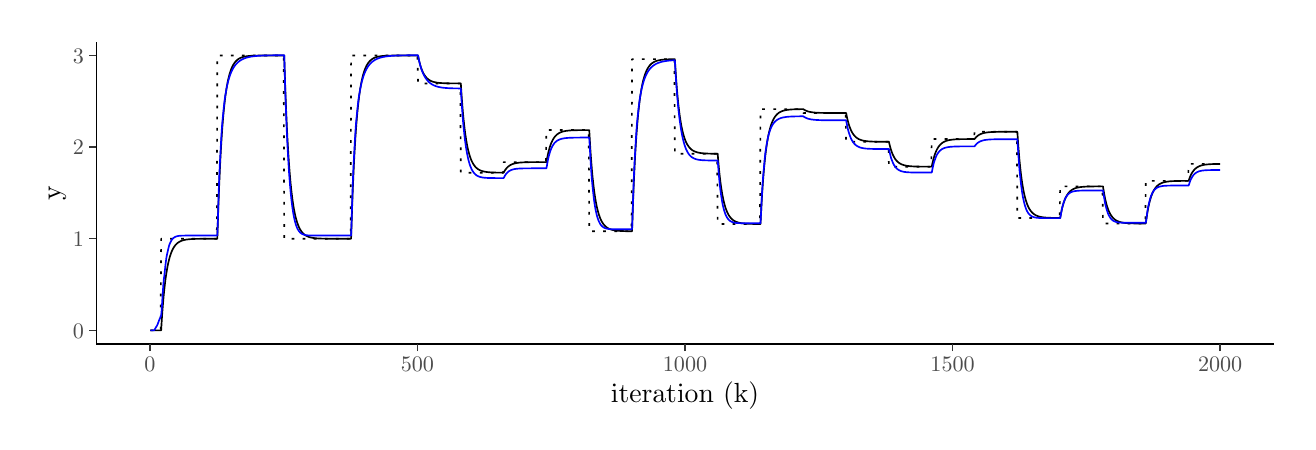
\begin{tikzpicture}[x=1pt,y=1pt]
\definecolor{fillColor}{RGB}{255,255,255}
\path[use as bounding box,fill=fillColor,fill opacity=0.00] (0,0) rectangle (455.24,142.26);
\begin{scope}
\path[clip] (  0.00,  0.00) rectangle (455.24,142.26);
\definecolor{drawColor}{RGB}{255,255,255}
\definecolor{fillColor}{RGB}{255,255,255}

\path[draw=drawColor,line width= 0.5pt,line join=round,line cap=round,fill=fillColor] (  0.00,  0.00) rectangle (455.24,142.26);
\end{scope}
\begin{scope}
\path[clip] ( 24.83, 27.90) rectangle (450.24,137.26);
\definecolor{fillColor}{RGB}{255,255,255}

\path[fill=fillColor] ( 24.83, 27.90) rectangle (450.24,137.26);
\definecolor{drawColor}{RGB}{0,0,0}

\path[draw=drawColor,line width= 0.6pt,dash pattern=on 1pt off 3pt ,line join=round] ( 44.36, 32.87) --
	( 44.55, 32.87) --
	( 44.75, 32.87) --
	( 44.94, 32.87) --
	( 45.13, 32.87) --
	( 45.33, 32.87) --
	( 45.52, 32.87) --
	( 45.71, 32.87) --
	( 45.91, 32.87) --
	( 46.10, 32.87) --
	( 46.29, 32.87) --
	( 46.49, 32.87) --
	( 46.68, 32.87) --
	( 46.87, 32.87) --
	( 47.07, 32.87) --
	( 47.26, 32.87) --
	( 47.45, 32.87) --
	( 47.65, 32.87) --
	( 47.84, 32.87) --
	( 48.03, 32.87) --
	( 48.23, 65.98) --
	( 48.42, 65.98) --
	( 48.61, 65.98) --
	( 48.81, 65.98) --
	( 49.00, 65.98) --
	( 49.19, 65.98) --
	( 49.39, 65.98) --
	( 49.58, 65.98) --
	( 49.77, 65.98) --
	( 49.97, 65.98) --
	( 50.16, 65.98) --
	( 50.36, 65.98) --
	( 50.55, 65.98) --
	( 50.74, 65.98) --
	( 50.94, 65.98) --
	( 51.13, 65.98) --
	( 51.32, 65.98) --
	( 51.52, 65.98) --
	( 51.71, 65.98) --
	( 51.90, 65.98) --
	( 52.10, 65.98) --
	( 52.29, 65.98) --
	( 52.48, 65.98) --
	( 52.68, 65.98) --
	( 52.87, 65.98) --
	( 53.06, 65.98) --
	( 53.26, 65.98) --
	( 53.45, 65.98) --
	( 53.64, 65.98) --
	( 53.84, 65.98) --
	( 54.03, 65.98) --
	( 54.22, 65.98) --
	( 54.42, 65.98) --
	( 54.61, 65.98) --
	( 54.80, 65.98) --
	( 55.00, 65.98) --
	( 55.19, 65.98) --
	( 55.38, 65.98) --
	( 55.58, 65.98) --
	( 55.77, 65.98) --
	( 55.96, 65.98) --
	( 56.16, 65.98) --
	( 56.35, 65.98) --
	( 56.54, 65.98) --
	( 56.74, 65.98) --
	( 56.93, 65.98) --
	( 57.12, 65.98) --
	( 57.32, 65.98) --
	( 57.51, 65.98) --
	( 57.70, 65.98) --
	( 57.90, 65.98) --
	( 58.09, 65.98) --
	( 58.28, 65.98) --
	( 58.48, 65.98) --
	( 58.67, 65.98) --
	( 58.86, 65.98) --
	( 59.06, 65.98) --
	( 59.25, 65.98) --
	( 59.44, 65.98) --
	( 59.64, 65.98) --
	( 59.83, 65.98) --
	( 60.02, 65.98) --
	( 60.22, 65.98) --
	( 60.41, 65.98) --
	( 60.60, 65.98) --
	( 60.80, 65.98) --
	( 60.99, 65.98) --
	( 61.18, 65.98) --
	( 61.38, 65.98) --
	( 61.57, 65.98) --
	( 61.76, 65.98) --
	( 61.96, 65.98) --
	( 62.15, 65.98) --
	( 62.34, 65.98) --
	( 62.54, 65.98) --
	( 62.73, 65.98) --
	( 62.92, 65.98) --
	( 63.12, 65.98) --
	( 63.31, 65.98) --
	( 63.50, 65.98) --
	( 63.70, 65.98) --
	( 63.89, 65.98) --
	( 64.08, 65.98) --
	( 64.28, 65.98) --
	( 64.47, 65.98) --
	( 64.66, 65.98) --
	( 64.86, 65.98) --
	( 65.05, 65.98) --
	( 65.24, 65.98) --
	( 65.44, 65.98) --
	( 65.63, 65.98) --
	( 65.82, 65.98) --
	( 66.02, 65.98) --
	( 66.21, 65.98) --
	( 66.40, 65.98) --
	( 66.60, 65.98) --
	( 66.79, 65.98) --
	( 66.98, 65.98) --
	( 67.18, 65.98) --
	( 67.37, 65.98) --
	( 67.56, 65.98) --
	( 67.76, 65.98) --
	( 67.95, 65.98) --
	( 68.15, 65.98) --
	( 68.34, 65.98) --
	( 68.53,132.21) --
	( 68.73,132.21) --
	( 68.92,132.21) --
	( 69.11,132.21) --
	( 69.31,132.21) --
	( 69.50,132.21) --
	( 69.69,132.21) --
	( 69.89,132.21) --
	( 70.08,132.21) --
	( 70.27,132.21) --
	( 70.47,132.21) --
	( 70.66,132.21) --
	( 70.85,132.21) --
	( 71.05,132.21) --
	( 71.24,132.21) --
	( 71.43,132.21) --
	( 71.63,132.21) --
	( 71.82,132.21) --
	( 72.01,132.21) --
	( 72.21,132.21) --
	( 72.40,132.21) --
	( 72.59,132.21) --
	( 72.79,132.21) --
	( 72.98,132.21) --
	( 73.17,132.21) --
	( 73.37,132.21) --
	( 73.56,132.21) --
	( 73.75,132.21) --
	( 73.95,132.21) --
	( 74.14,132.21) --
	( 74.33,132.21) --
	( 74.53,132.21) --
	( 74.72,132.21) --
	( 74.91,132.21) --
	( 75.11,132.21) --
	( 75.30,132.21) --
	( 75.49,132.21) --
	( 75.69,132.21) --
	( 75.88,132.21) --
	( 76.07,132.21) --
	( 76.27,132.21) --
	( 76.46,132.21) --
	( 76.65,132.21) --
	( 76.85,132.21) --
	( 77.04,132.21) --
	( 77.23,132.21) --
	( 77.43,132.21) --
	( 77.62,132.21) --
	( 77.81,132.21) --
	( 78.01,132.21) --
	( 78.20,132.21) --
	( 78.39,132.21) --
	( 78.59,132.21) --
	( 78.78,132.21) --
	( 78.97,132.21) --
	( 79.17,132.21) --
	( 79.36,132.21) --
	( 79.55,132.21) --
	( 79.75,132.21) --
	( 79.94,132.21) --
	( 80.13,132.21) --
	( 80.33,132.21) --
	( 80.52,132.21) --
	( 80.71,132.21) --
	( 80.91,132.21) --
	( 81.10,132.21) --
	( 81.29,132.21) --
	( 81.49,132.21) --
	( 81.68,132.21) --
	( 81.87,132.21) --
	( 82.07,132.21) --
	( 82.26,132.21) --
	( 82.45,132.21) --
	( 82.65,132.21) --
	( 82.84,132.21) --
	( 83.03,132.21) --
	( 83.23,132.21) --
	( 83.42,132.21) --
	( 83.61,132.21) --
	( 83.81,132.21) --
	( 84.00,132.21) --
	( 84.19,132.21) --
	( 84.39,132.21) --
	( 84.58,132.21) --
	( 84.77,132.21) --
	( 84.97,132.21) --
	( 85.16,132.21) --
	( 85.36,132.21) --
	( 85.55,132.21) --
	( 85.74,132.21) --
	( 85.94,132.21) --
	( 86.13,132.21) --
	( 86.32,132.21) --
	( 86.52,132.21) --
	( 86.71,132.21) --
	( 86.90,132.21) --
	( 87.10,132.21) --
	( 87.29,132.21) --
	( 87.48,132.21) --
	( 87.68,132.21) --
	( 87.87,132.21) --
	( 88.06,132.21) --
	( 88.26,132.21) --
	( 88.45,132.21) --
	( 88.64,132.21) --
	( 88.84,132.21) --
	( 89.03,132.21) --
	( 89.22,132.21) --
	( 89.42,132.21) --
	( 89.61,132.21) --
	( 89.80,132.21) --
	( 90.00,132.21) --
	( 90.19,132.21) --
	( 90.38,132.21) --
	( 90.58,132.21) --
	( 90.77,132.21) --
	( 90.96,132.21) --
	( 91.16,132.21) --
	( 91.35,132.21) --
	( 91.54,132.21) --
	( 91.74,132.21) --
	( 91.93,132.21) --
	( 92.12,132.21) --
	( 92.32,132.21) --
	( 92.51,132.21) --
	( 92.70, 65.98) --
	( 92.90, 65.98) --
	( 93.09, 65.98) --
	( 93.28, 65.98) --
	( 93.48, 65.98) --
	( 93.67, 65.98) --
	( 93.86, 65.98) --
	( 94.06, 65.98) --
	( 94.25, 65.98) --
	( 94.44, 65.98) --
	( 94.64, 65.98) --
	( 94.83, 65.98) --
	( 95.02, 65.98) --
	( 95.22, 65.98) --
	( 95.41, 65.98) --
	( 95.60, 65.98) --
	( 95.80, 65.98) --
	( 95.99, 65.98) --
	( 96.18, 65.98) --
	( 96.38, 65.98) --
	( 96.57, 65.98) --
	( 96.76, 65.98) --
	( 96.96, 65.98) --
	( 97.15, 65.98) --
	( 97.34, 65.98) --
	( 97.54, 65.98) --
	( 97.73, 65.98) --
	( 97.92, 65.98) --
	( 98.12, 65.98) --
	( 98.31, 65.98) --
	( 98.50, 65.98) --
	( 98.70, 65.98) --
	( 98.89, 65.98) --
	( 99.08, 65.98) --
	( 99.28, 65.98) --
	( 99.47, 65.98) --
	( 99.66, 65.98) --
	( 99.86, 65.98) --
	(100.05, 65.98) --
	(100.24, 65.98) --
	(100.44, 65.98) --
	(100.63, 65.98) --
	(100.82, 65.98) --
	(101.02, 65.98) --
	(101.21, 65.98) --
	(101.40, 65.98) --
	(101.60, 65.98) --
	(101.79, 65.98) --
	(101.98, 65.98) --
	(102.18, 65.98) --
	(102.37, 65.98) --
	(102.56, 65.98) --
	(102.76, 65.98) --
	(102.95, 65.98) --
	(103.15, 65.98) --
	(103.34, 65.98) --
	(103.53, 65.98) --
	(103.73, 65.98) --
	(103.92, 65.98) --
	(104.11, 65.98) --
	(104.31, 65.98) --
	(104.50, 65.98) --
	(104.69, 65.98) --
	(104.89, 65.98) --
	(105.08, 65.98) --
	(105.27, 65.98) --
	(105.47, 65.98) --
	(105.66, 65.98) --
	(105.85, 65.98) --
	(106.05, 65.98) --
	(106.24, 65.98) --
	(106.43, 65.98) --
	(106.63, 65.98) --
	(106.82, 65.98) --
	(107.01, 65.98) --
	(107.21, 65.98) --
	(107.40, 65.98) --
	(107.59, 65.98) --
	(107.79, 65.98) --
	(107.98, 65.98) --
	(108.17, 65.98) --
	(108.37, 65.98) --
	(108.56, 65.98) --
	(108.75, 65.98) --
	(108.95, 65.98) --
	(109.14, 65.98) --
	(109.33, 65.98) --
	(109.53, 65.98) --
	(109.72, 65.98) --
	(109.91, 65.98) --
	(110.11, 65.98) --
	(110.30, 65.98) --
	(110.49, 65.98) --
	(110.69, 65.98) --
	(110.88, 65.98) --
	(111.07, 65.98) --
	(111.27, 65.98) --
	(111.46, 65.98) --
	(111.65, 65.98) --
	(111.85, 65.98) --
	(112.04, 65.98) --
	(112.23, 65.98) --
	(112.43, 65.98) --
	(112.62, 65.98) --
	(112.81, 65.98) --
	(113.01, 65.98) --
	(113.20, 65.98) --
	(113.39, 65.98) --
	(113.59, 65.98) --
	(113.78, 65.98) --
	(113.97, 65.98) --
	(114.17, 65.98) --
	(114.36, 65.98) --
	(114.55, 65.98) --
	(114.75, 65.98) --
	(114.94, 65.98) --
	(115.13, 65.98) --
	(115.33, 65.98) --
	(115.52, 65.98) --
	(115.71, 65.98) --
	(115.91, 65.98) --
	(116.10, 65.98) --
	(116.29, 65.98) --
	(116.49, 65.98) --
	(116.68, 65.98) --
	(116.87,132.21) --
	(117.07,132.21) --
	(117.26,132.21) --
	(117.45,132.21) --
	(117.65,132.21) --
	(117.84,132.21) --
	(118.03,132.21) --
	(118.23,132.21) --
	(118.42,132.21) --
	(118.61,132.21) --
	(118.81,132.21) --
	(119.00,132.21) --
	(119.19,132.21) --
	(119.39,132.21) --
	(119.58,132.21) --
	(119.77,132.21) --
	(119.97,132.21) --
	(120.16,132.21) --
	(120.36,132.21) --
	(120.55,132.21) --
	(120.74,132.21) --
	(120.94,132.21) --
	(121.13,132.21) --
	(121.32,132.21) --
	(121.52,132.21) --
	(121.71,132.21) --
	(121.90,132.21) --
	(122.10,132.21) --
	(122.29,132.21) --
	(122.48,132.21) --
	(122.68,132.21) --
	(122.87,132.21) --
	(123.06,132.21) --
	(123.26,132.21) --
	(123.45,132.21) --
	(123.64,132.21) --
	(123.84,132.21) --
	(124.03,132.21) --
	(124.22,132.21) --
	(124.42,132.21) --
	(124.61,132.21) --
	(124.80,132.21) --
	(125.00,132.21) --
	(125.19,132.21) --
	(125.38,132.21) --
	(125.58,132.21) --
	(125.77,132.21) --
	(125.96,132.21) --
	(126.16,132.21) --
	(126.35,132.21) --
	(126.54,132.21) --
	(126.74,132.21) --
	(126.93,132.21) --
	(127.12,132.21) --
	(127.32,132.21) --
	(127.51,132.21) --
	(127.70,132.21) --
	(127.90,132.21) --
	(128.09,132.21) --
	(128.28,132.21) --
	(128.48,132.21) --
	(128.67,132.21) --
	(128.86,132.21) --
	(129.06,132.21) --
	(129.25,132.21) --
	(129.44,132.21) --
	(129.64,132.21) --
	(129.83,132.21) --
	(130.02,132.21) --
	(130.22,132.21) --
	(130.41,132.21) --
	(130.60,132.21) --
	(130.80,132.21) --
	(130.99,132.21) --
	(131.18,132.21) --
	(131.38,132.21) --
	(131.57,132.21) --
	(131.76,132.21) --
	(131.96,132.21) --
	(132.15,132.21) --
	(132.34,132.21) --
	(132.54,132.21) --
	(132.73,132.21) --
	(132.92,132.21) --
	(133.12,132.21) --
	(133.31,132.21) --
	(133.50,132.21) --
	(133.70,132.21) --
	(133.89,132.21) --
	(134.08,132.21) --
	(134.28,132.21) --
	(134.47,132.21) --
	(134.66,132.21) --
	(134.86,132.21) --
	(135.05,132.21) --
	(135.24,132.21) --
	(135.44,132.21) --
	(135.63,132.21) --
	(135.82,132.21) --
	(136.02,132.21) --
	(136.21,132.21) --
	(136.40,132.21) --
	(136.60,132.21) --
	(136.79,132.21) --
	(136.98,132.21) --
	(137.18,132.21) --
	(137.37,132.21) --
	(137.56,132.21) --
	(137.76,132.21) --
	(137.95,132.21) --
	(138.15,132.21) --
	(138.34,132.21) --
	(138.53,132.21) --
	(138.73,132.21) --
	(138.92,132.21) --
	(139.11,132.21) --
	(139.31,132.21) --
	(139.50,132.21) --
	(139.69,132.21) --
	(139.89,132.21) --
	(140.08,132.21) --
	(140.27,132.21) --
	(140.47,132.21) --
	(140.66,132.21) --
	(140.85,132.21) --
	(141.05,122.11) --
	(141.24,122.11) --
	(141.43,122.11) --
	(141.63,122.11) --
	(141.82,122.11) --
	(142.01,122.11) --
	(142.21,122.11) --
	(142.40,122.11) --
	(142.59,122.11) --
	(142.79,122.11) --
	(142.98,122.11) --
	(143.17,122.11) --
	(143.37,122.11) --
	(143.56,122.11) --
	(143.75,122.11) --
	(143.95,122.11) --
	(144.14,122.11) --
	(144.33,122.11) --
	(144.53,122.11) --
	(144.72,122.11) --
	(144.91,122.11) --
	(145.11,122.11) --
	(145.30,122.11) --
	(145.49,122.11) --
	(145.69,122.11) --
	(145.88,122.11) --
	(146.07,122.11) --
	(146.27,122.11) --
	(146.46,122.11) --
	(146.65,122.11) --
	(146.85,122.11) --
	(147.04,122.11) --
	(147.23,122.11) --
	(147.43,122.11) --
	(147.62,122.11) --
	(147.81,122.11) --
	(148.01,122.11) --
	(148.20,122.11) --
	(148.39,122.11) --
	(148.59,122.11) --
	(148.78,122.11) --
	(148.97,122.11) --
	(149.17,122.11) --
	(149.36,122.11) --
	(149.55,122.11) --
	(149.75,122.11) --
	(149.94,122.11) --
	(150.13,122.11) --
	(150.33,122.11) --
	(150.52,122.11) --
	(150.71,122.11) --
	(150.91,122.11) --
	(151.10,122.11) --
	(151.29,122.11) --
	(151.49,122.11) --
	(151.68,122.11) --
	(151.87,122.11) --
	(152.07,122.11) --
	(152.26,122.11) --
	(152.45,122.11) --
	(152.65,122.11) --
	(152.84,122.11) --
	(153.03,122.11) --
	(153.23,122.11) --
	(153.42,122.11) --
	(153.61,122.11) --
	(153.81,122.11) --
	(154.00,122.11) --
	(154.19,122.11) --
	(154.39,122.11) --
	(154.58,122.11) --
	(154.77,122.11) --
	(154.97,122.11) --
	(155.16,122.11) --
	(155.35,122.11) --
	(155.55,122.11) --
	(155.74,122.11) --
	(155.94,122.11) --
	(156.13,122.11) --
	(156.32,122.11) --
	(156.52, 89.85) --
	(156.71, 89.85) --
	(156.90, 89.85) --
	(157.10, 89.85) --
	(157.29, 89.85) --
	(157.48, 89.85) --
	(157.68, 89.85) --
	(157.87, 89.85) --
	(158.06, 89.85) --
	(158.26, 89.85) --
	(158.45, 89.85) --
	(158.64, 89.85) --
	(158.84, 89.85) --
	(159.03, 89.85) --
	(159.22, 89.85) --
	(159.42, 89.85) --
	(159.61, 89.85) --
	(159.80, 89.85) --
	(160.00, 89.85) --
	(160.19, 89.85) --
	(160.38, 89.85) --
	(160.58, 89.85) --
	(160.77, 89.85) --
	(160.96, 89.85) --
	(161.16, 89.85) --
	(161.35, 89.85) --
	(161.54, 89.85) --
	(161.74, 89.85) --
	(161.93, 89.85) --
	(162.12, 89.85) --
	(162.32, 89.85) --
	(162.51, 89.85) --
	(162.70, 89.85) --
	(162.90, 89.85) --
	(163.09, 89.85) --
	(163.28, 89.85) --
	(163.48, 89.85) --
	(163.67, 89.85) --
	(163.86, 89.85) --
	(164.06, 89.85) --
	(164.25, 89.85) --
	(164.44, 89.85) --
	(164.64, 89.85) --
	(164.83, 89.85) --
	(165.02, 89.85) --
	(165.22, 89.85) --
	(165.41, 89.85) --
	(165.60, 89.85) --
	(165.80, 89.85) --
	(165.99, 89.85) --
	(166.18, 89.85) --
	(166.38, 89.85) --
	(166.57, 89.85) --
	(166.76, 89.85) --
	(166.96, 89.85) --
	(167.15, 89.85) --
	(167.34, 89.85) --
	(167.54, 89.85) --
	(167.73, 89.85) --
	(167.92, 89.85) --
	(168.12, 89.85) --
	(168.31, 89.85) --
	(168.50, 89.85) --
	(168.70, 89.85) --
	(168.89, 89.85) --
	(169.08, 89.85) --
	(169.28, 89.85) --
	(169.47, 89.85) --
	(169.66, 89.85) --
	(169.86, 89.85) --
	(170.05, 89.85) --
	(170.24, 89.85) --
	(170.44, 89.85) --
	(170.63, 89.85) --
	(170.82, 89.85) --
	(171.02, 89.85) --
	(171.21, 89.85) --
	(171.40, 89.85) --
	(171.60, 89.85) --
	(171.79, 89.85) --
	(171.98, 93.69) --
	(172.18, 93.69) --
	(172.37, 93.69) --
	(172.56, 93.69) --
	(172.76, 93.69) --
	(172.95, 93.69) --
	(173.15, 93.69) --
	(173.34, 93.69) --
	(173.53, 93.69) --
	(173.73, 93.69) --
	(173.92, 93.69) --
	(174.11, 93.69) --
	(174.31, 93.69) --
	(174.50, 93.69) --
	(174.69, 93.69) --
	(174.89, 93.69) --
	(175.08, 93.69) --
	(175.27, 93.69) --
	(175.47, 93.69) --
	(175.66, 93.69) --
	(175.85, 93.69) --
	(176.05, 93.69) --
	(176.24, 93.69) --
	(176.43, 93.69) --
	(176.63, 93.69) --
	(176.82, 93.69) --
	(177.01, 93.69) --
	(177.21, 93.69) --
	(177.40, 93.69) --
	(177.59, 93.69) --
	(177.79, 93.69) --
	(177.98, 93.69) --
	(178.17, 93.69) --
	(178.37, 93.69) --
	(178.56, 93.69) --
	(178.75, 93.69) --
	(178.95, 93.69) --
	(179.14, 93.69) --
	(179.33, 93.69) --
	(179.53, 93.69) --
	(179.72, 93.69) --
	(179.91, 93.69) --
	(180.11, 93.69) --
	(180.30, 93.69) --
	(180.49, 93.69) --
	(180.69, 93.69) --
	(180.88, 93.69) --
	(181.07, 93.69) --
	(181.27, 93.69) --
	(181.46, 93.69) --
	(181.65, 93.69) --
	(181.85, 93.69) --
	(182.04, 93.69) --
	(182.23, 93.69) --
	(182.43, 93.69) --
	(182.62, 93.69) --
	(182.81, 93.69) --
	(183.01, 93.69) --
	(183.20, 93.69) --
	(183.39, 93.69) --
	(183.59, 93.69) --
	(183.78, 93.69) --
	(183.97, 93.69) --
	(184.17, 93.69) --
	(184.36, 93.69) --
	(184.55, 93.69) --
	(184.75, 93.69) --
	(184.94, 93.69) --
	(185.13, 93.69) --
	(185.33, 93.69) --
	(185.52, 93.69) --
	(185.71, 93.69) --
	(185.91, 93.69) --
	(186.10, 93.69) --
	(186.29, 93.69) --
	(186.49, 93.69) --
	(186.68, 93.69) --
	(186.87, 93.69) --
	(187.07, 93.69) --
	(187.26, 93.69) --
	(187.45,105.26) --
	(187.65,105.26) --
	(187.84,105.26) --
	(188.03,105.26) --
	(188.23,105.26) --
	(188.42,105.26) --
	(188.61,105.26) --
	(188.81,105.26) --
	(189.00,105.26) --
	(189.19,105.26) --
	(189.39,105.26) --
	(189.58,105.26) --
	(189.77,105.26) --
	(189.97,105.26) --
	(190.16,105.26) --
	(190.35,105.26) --
	(190.55,105.26) --
	(190.74,105.26) --
	(190.94,105.26) --
	(191.13,105.26) --
	(191.32,105.26) --
	(191.52,105.26) --
	(191.71,105.26) --
	(191.90,105.26) --
	(192.10,105.26) --
	(192.29,105.26) --
	(192.48,105.26) --
	(192.68,105.26) --
	(192.87,105.26) --
	(193.06,105.26) --
	(193.26,105.26) --
	(193.45,105.26) --
	(193.64,105.26) --
	(193.84,105.26) --
	(194.03,105.26) --
	(194.22,105.26) --
	(194.42,105.26) --
	(194.61,105.26) --
	(194.80,105.26) --
	(195.00,105.26) --
	(195.19,105.26) --
	(195.38,105.26) --
	(195.58,105.26) --
	(195.77,105.26) --
	(195.96,105.26) --
	(196.16,105.26) --
	(196.35,105.26) --
	(196.54,105.26) --
	(196.74,105.26) --
	(196.93,105.26) --
	(197.12,105.26) --
	(197.32,105.26) --
	(197.51,105.26) --
	(197.70,105.26) --
	(197.90,105.26) --
	(198.09,105.26) --
	(198.28,105.26) --
	(198.48,105.26) --
	(198.67,105.26) --
	(198.86,105.26) --
	(199.06,105.26) --
	(199.25,105.26) --
	(199.44,105.26) --
	(199.64,105.26) --
	(199.83,105.26) --
	(200.02,105.26) --
	(200.22,105.26) --
	(200.41,105.26) --
	(200.60,105.26) --
	(200.80,105.26) --
	(200.99,105.26) --
	(201.18,105.26) --
	(201.38,105.26) --
	(201.57,105.26) --
	(201.76,105.26) --
	(201.96,105.26) --
	(202.15,105.26) --
	(202.34,105.26) --
	(202.54,105.26) --
	(202.73,105.26) --
	(202.92, 68.70) --
	(203.12, 68.70) --
	(203.31, 68.70) --
	(203.50, 68.70) --
	(203.70, 68.70) --
	(203.89, 68.70) --
	(204.08, 68.70) --
	(204.28, 68.70) --
	(204.47, 68.70) --
	(204.66, 68.70) --
	(204.86, 68.70) --
	(205.05, 68.70) --
	(205.24, 68.70) --
	(205.44, 68.70) --
	(205.63, 68.70) --
	(205.82, 68.70) --
	(206.02, 68.70) --
	(206.21, 68.70) --
	(206.40, 68.70) --
	(206.60, 68.70) --
	(206.79, 68.70) --
	(206.98, 68.70) --
	(207.18, 68.70) --
	(207.37, 68.70) --
	(207.56, 68.70) --
	(207.76, 68.70) --
	(207.95, 68.70) --
	(208.15, 68.70) --
	(208.34, 68.70) --
	(208.53, 68.70) --
	(208.73, 68.70) --
	(208.92, 68.70) --
	(209.11, 68.70) --
	(209.31, 68.70) --
	(209.50, 68.70) --
	(209.69, 68.70) --
	(209.89, 68.70) --
	(210.08, 68.70) --
	(210.27, 68.70) --
	(210.47, 68.70) --
	(210.66, 68.70) --
	(210.85, 68.70) --
	(211.05, 68.70) --
	(211.24, 68.70) --
	(211.43, 68.70) --
	(211.63, 68.70) --
	(211.82, 68.70) --
	(212.01, 68.70) --
	(212.21, 68.70) --
	(212.40, 68.70) --
	(212.59, 68.70) --
	(212.79, 68.70) --
	(212.98, 68.70) --
	(213.17, 68.70) --
	(213.37, 68.70) --
	(213.56, 68.70) --
	(213.75, 68.70) --
	(213.95, 68.70) --
	(214.14, 68.70) --
	(214.33, 68.70) --
	(214.53, 68.70) --
	(214.72, 68.70) --
	(214.91, 68.70) --
	(215.11, 68.70) --
	(215.30, 68.70) --
	(215.49, 68.70) --
	(215.69, 68.70) --
	(215.88, 68.70) --
	(216.07, 68.70) --
	(216.27, 68.70) --
	(216.46, 68.70) --
	(216.65, 68.70) --
	(216.85, 68.70) --
	(217.04, 68.70) --
	(217.23, 68.70) --
	(217.43, 68.70) --
	(217.62, 68.70) --
	(217.81, 68.70) --
	(218.01, 68.70) --
	(218.20, 68.70) --
	(218.39,130.89) --
	(218.59,130.89) --
	(218.78,130.89) --
	(218.97,130.89) --
	(219.17,130.89) --
	(219.36,130.89) --
	(219.55,130.89) --
	(219.75,130.89) --
	(219.94,130.89) --
	(220.13,130.89) --
	(220.33,130.89) --
	(220.52,130.89) --
	(220.71,130.89) --
	(220.91,130.89) --
	(221.10,130.89) --
	(221.29,130.89) --
	(221.49,130.89) --
	(221.68,130.89) --
	(221.87,130.89) --
	(222.07,130.89) --
	(222.26,130.89) --
	(222.45,130.89) --
	(222.65,130.89) --
	(222.84,130.89) --
	(223.03,130.89) --
	(223.23,130.89) --
	(223.42,130.89) --
	(223.61,130.89) --
	(223.81,130.89) --
	(224.00,130.89) --
	(224.19,130.89) --
	(224.39,130.89) --
	(224.58,130.89) --
	(224.77,130.89) --
	(224.97,130.89) --
	(225.16,130.89) --
	(225.35,130.89) --
	(225.55,130.89) --
	(225.74,130.89) --
	(225.94,130.89) --
	(226.13,130.89) --
	(226.32,130.89) --
	(226.52,130.89) --
	(226.71,130.89) --
	(226.90,130.89) --
	(227.10,130.89) --
	(227.29,130.89) --
	(227.48,130.89) --
	(227.68,130.89) --
	(227.87,130.89) --
	(228.06,130.89) --
	(228.26,130.89) --
	(228.45,130.89) --
	(228.64,130.89) --
	(228.84,130.89) --
	(229.03,130.89) --
	(229.22,130.89) --
	(229.42,130.89) --
	(229.61,130.89) --
	(229.80,130.89) --
	(230.00,130.89) --
	(230.19,130.89) --
	(230.38,130.89) --
	(230.58,130.89) --
	(230.77,130.89) --
	(230.96,130.89) --
	(231.16,130.89) --
	(231.35,130.89) --
	(231.54,130.89) --
	(231.74,130.89) --
	(231.93,130.89) --
	(232.12,130.89) --
	(232.32,130.89) --
	(232.51,130.89) --
	(232.70,130.89) --
	(232.90,130.89) --
	(233.09,130.89) --
	(233.28,130.89) --
	(233.48,130.89) --
	(233.67,130.89) --
	(233.86, 96.69) --
	(234.06, 96.69) --
	(234.25, 96.69) --
	(234.44, 96.69) --
	(234.64, 96.69) --
	(234.83, 96.69) --
	(235.02, 96.69) --
	(235.22, 96.69) --
	(235.41, 96.69) --
	(235.60, 96.69) --
	(235.80, 96.69) --
	(235.99, 96.69) --
	(236.18, 96.69) --
	(236.38, 96.69) --
	(236.57, 96.69) --
	(236.76, 96.69) --
	(236.96, 96.69) --
	(237.15, 96.69) --
	(237.34, 96.69) --
	(237.54, 96.69) --
	(237.73, 96.69) --
	(237.92, 96.69) --
	(238.12, 96.69) --
	(238.31, 96.69) --
	(238.50, 96.69) --
	(238.70, 96.69) --
	(238.89, 96.69) --
	(239.08, 96.69) --
	(239.28, 96.69) --
	(239.47, 96.69) --
	(239.66, 96.69) --
	(239.86, 96.69) --
	(240.05, 96.69) --
	(240.24, 96.69) --
	(240.44, 96.69) --
	(240.63, 96.69) --
	(240.82, 96.69) --
	(241.02, 96.69) --
	(241.21, 96.69) --
	(241.40, 96.69) --
	(241.60, 96.69) --
	(241.79, 96.69) --
	(241.98, 96.69) --
	(242.18, 96.69) --
	(242.37, 96.69) --
	(242.56, 96.69) --
	(242.76, 96.69) --
	(242.95, 96.69) --
	(243.14, 96.69) --
	(243.34, 96.69) --
	(243.53, 96.69) --
	(243.73, 96.69) --
	(243.92, 96.69) --
	(244.11, 96.69) --
	(244.31, 96.69) --
	(244.50, 96.69) --
	(244.69, 96.69) --
	(244.89, 96.69) --
	(245.08, 96.69) --
	(245.27, 96.69) --
	(245.47, 96.69) --
	(245.66, 96.69) --
	(245.85, 96.69) --
	(246.05, 96.69) --
	(246.24, 96.69) --
	(246.43, 96.69) --
	(246.63, 96.69) --
	(246.82, 96.69) --
	(247.01, 96.69) --
	(247.21, 96.69) --
	(247.40, 96.69) --
	(247.59, 96.69) --
	(247.79, 96.69) --
	(247.98, 96.69) --
	(248.17, 96.69) --
	(248.37, 96.69) --
	(248.56, 96.69) --
	(248.75, 96.69) --
	(248.95, 96.69) --
	(249.14, 96.69) --
	(249.33, 71.31) --
	(249.53, 71.31) --
	(249.72, 71.31) --
	(249.91, 71.31) --
	(250.11, 71.31) --
	(250.30, 71.31) --
	(250.49, 71.31) --
	(250.69, 71.31) --
	(250.88, 71.31) --
	(251.07, 71.31) --
	(251.27, 71.31) --
	(251.46, 71.31) --
	(251.65, 71.31) --
	(251.85, 71.31) --
	(252.04, 71.31) --
	(252.23, 71.31) --
	(252.43, 71.31) --
	(252.62, 71.31) --
	(252.81, 71.31) --
	(253.01, 71.31) --
	(253.20, 71.31) --
	(253.39, 71.31) --
	(253.59, 71.31) --
	(253.78, 71.31) --
	(253.97, 71.31) --
	(254.17, 71.31) --
	(254.36, 71.31) --
	(254.55, 71.31) --
	(254.75, 71.31) --
	(254.94, 71.31) --
	(255.13, 71.31) --
	(255.33, 71.31) --
	(255.52, 71.31) --
	(255.71, 71.31) --
	(255.91, 71.31) --
	(256.10, 71.31) --
	(256.29, 71.31) --
	(256.49, 71.31) --
	(256.68, 71.31) --
	(256.87, 71.31) --
	(257.07, 71.31) --
	(257.26, 71.31) --
	(257.45, 71.31) --
	(257.65, 71.31) --
	(257.84, 71.31) --
	(258.03, 71.31) --
	(258.23, 71.31) --
	(258.42, 71.31) --
	(258.61, 71.31) --
	(258.81, 71.31) --
	(259.00, 71.31) --
	(259.19, 71.31) --
	(259.39, 71.31) --
	(259.58, 71.31) --
	(259.77, 71.31) --
	(259.97, 71.31) --
	(260.16, 71.31) --
	(260.35, 71.31) --
	(260.55, 71.31) --
	(260.74, 71.31) --
	(260.94, 71.31) --
	(261.13, 71.31) --
	(261.32, 71.31) --
	(261.52, 71.31) --
	(261.71, 71.31) --
	(261.90, 71.31) --
	(262.10, 71.31) --
	(262.29, 71.31) --
	(262.48, 71.31) --
	(262.68, 71.31) --
	(262.87, 71.31) --
	(263.06, 71.31) --
	(263.26, 71.31) --
	(263.45, 71.31) --
	(263.64, 71.31) --
	(263.84, 71.31) --
	(264.03, 71.31) --
	(264.22, 71.31) --
	(264.42, 71.31) --
	(264.61, 71.31) --
	(264.80,112.83) --
	(265.00,112.83) --
	(265.19,112.83) --
	(265.38,112.83) --
	(265.58,112.83) --
	(265.77,112.83) --
	(265.96,112.83) --
	(266.16,112.83) --
	(266.35,112.83) --
	(266.54,112.83) --
	(266.74,112.83) --
	(266.93,112.83) --
	(267.12,112.83) --
	(267.32,112.83) --
	(267.51,112.83) --
	(267.70,112.83) --
	(267.90,112.83) --
	(268.09,112.83) --
	(268.28,112.83) --
	(268.48,112.83) --
	(268.67,112.83) --
	(268.86,112.83) --
	(269.06,112.83) --
	(269.25,112.83) --
	(269.44,112.83) --
	(269.64,112.83) --
	(269.83,112.83) --
	(270.02,112.83) --
	(270.22,112.83) --
	(270.41,112.83) --
	(270.60,112.83) --
	(270.80,112.83) --
	(270.99,112.83) --
	(271.18,112.83) --
	(271.38,112.83) --
	(271.57,112.83) --
	(271.76,112.83) --
	(271.96,112.83) --
	(272.15,112.83) --
	(272.34,112.83) --
	(272.54,112.83) --
	(272.73,112.83) --
	(272.92,112.83) --
	(273.12,112.83) --
	(273.31,112.83) --
	(273.50,112.83) --
	(273.70,112.83) --
	(273.89,112.83) --
	(274.08,112.83) --
	(274.28,112.83) --
	(274.47,112.83) --
	(274.66,112.83) --
	(274.86,112.83) --
	(275.05,112.83) --
	(275.24,112.83) --
	(275.44,112.83) --
	(275.63,112.83) --
	(275.82,112.83) --
	(276.02,112.83) --
	(276.21,112.83) --
	(276.40,112.83) --
	(276.60,112.83) --
	(276.79,112.83) --
	(276.98,112.83) --
	(277.18,112.83) --
	(277.37,112.83) --
	(277.56,112.83) --
	(277.76,112.83) --
	(277.95,112.83) --
	(278.14,112.83) --
	(278.34,112.83) --
	(278.53,112.83) --
	(278.73,112.83) --
	(278.92,112.83) --
	(279.11,112.83) --
	(279.31,112.83) --
	(279.50,112.83) --
	(279.69,112.83) --
	(279.89,112.83) --
	(280.08,112.83) --
	(280.27,111.42) --
	(280.47,111.42) --
	(280.66,111.42) --
	(280.85,111.42) --
	(281.05,111.42) --
	(281.24,111.42) --
	(281.43,111.42) --
	(281.63,111.42) --
	(281.82,111.42) --
	(282.01,111.42) --
	(282.21,111.42) --
	(282.40,111.42) --
	(282.59,111.42) --
	(282.79,111.42) --
	(282.98,111.42) --
	(283.17,111.42) --
	(283.37,111.42) --
	(283.56,111.42) --
	(283.75,111.42) --
	(283.95,111.42) --
	(284.14,111.42) --
	(284.33,111.42) --
	(284.53,111.42) --
	(284.72,111.42) --
	(284.91,111.42) --
	(285.11,111.42) --
	(285.30,111.42) --
	(285.49,111.42) --
	(285.69,111.42) --
	(285.88,111.42) --
	(286.07,111.42) --
	(286.27,111.42) --
	(286.46,111.42) --
	(286.65,111.42) --
	(286.85,111.42) --
	(287.04,111.42) --
	(287.23,111.42) --
	(287.43,111.42) --
	(287.62,111.42) --
	(287.81,111.42) --
	(288.01,111.42) --
	(288.20,111.42) --
	(288.39,111.42) --
	(288.59,111.42) --
	(288.78,111.42) --
	(288.97,111.42) --
	(289.17,111.42) --
	(289.36,111.42) --
	(289.55,111.42) --
	(289.75,111.42) --
	(289.94,111.42) --
	(290.13,111.42) --
	(290.33,111.42) --
	(290.52,111.42) --
	(290.71,111.42) --
	(290.91,111.42) --
	(291.10,111.42) --
	(291.29,111.42) --
	(291.49,111.42) --
	(291.68,111.42) --
	(291.87,111.42) --
	(292.07,111.42) --
	(292.26,111.42) --
	(292.45,111.42) --
	(292.65,111.42) --
	(292.84,111.42) --
	(293.03,111.42) --
	(293.23,111.42) --
	(293.42,111.42) --
	(293.61,111.42) --
	(293.81,111.42) --
	(294.00,111.42) --
	(294.19,111.42) --
	(294.39,111.42) --
	(294.58,111.42) --
	(294.77,111.42) --
	(294.97,111.42) --
	(295.16,111.42) --
	(295.35,111.42) --
	(295.55,111.42) --
	(295.74,101.02) --
	(295.94,101.02) --
	(296.13,101.02) --
	(296.32,101.02) --
	(296.52,101.02) --
	(296.71,101.02) --
	(296.90,101.02) --
	(297.10,101.02) --
	(297.29,101.02) --
	(297.48,101.02) --
	(297.68,101.02) --
	(297.87,101.02) --
	(298.06,101.02) --
	(298.26,101.02) --
	(298.45,101.02) --
	(298.64,101.02) --
	(298.84,101.02) --
	(299.03,101.02) --
	(299.22,101.02) --
	(299.42,101.02) --
	(299.61,101.02) --
	(299.80,101.02) --
	(300.00,101.02) --
	(300.19,101.02) --
	(300.38,101.02) --
	(300.58,101.02) --
	(300.77,101.02) --
	(300.96,101.02) --
	(301.16,101.02) --
	(301.35,101.02) --
	(301.54,101.02) --
	(301.74,101.02) --
	(301.93,101.02) --
	(302.12,101.02) --
	(302.32,101.02) --
	(302.51,101.02) --
	(302.70,101.02) --
	(302.90,101.02) --
	(303.09,101.02) --
	(303.28,101.02) --
	(303.48,101.02) --
	(303.67,101.02) --
	(303.86,101.02) --
	(304.06,101.02) --
	(304.25,101.02) --
	(304.44,101.02) --
	(304.64,101.02) --
	(304.83,101.02) --
	(305.02,101.02) --
	(305.22,101.02) --
	(305.41,101.02) --
	(305.60,101.02) --
	(305.80,101.02) --
	(305.99,101.02) --
	(306.18,101.02) --
	(306.38,101.02) --
	(306.57,101.02) --
	(306.76,101.02) --
	(306.96,101.02) --
	(307.15,101.02) --
	(307.34,101.02) --
	(307.54,101.02) --
	(307.73,101.02) --
	(307.92,101.02) --
	(308.12,101.02) --
	(308.31,101.02) --
	(308.50,101.02) --
	(308.70,101.02) --
	(308.89,101.02) --
	(309.08,101.02) --
	(309.28,101.02) --
	(309.47,101.02) --
	(309.66,101.02) --
	(309.86,101.02) --
	(310.05,101.02) --
	(310.24,101.02) --
	(310.44,101.02) --
	(310.63,101.02) --
	(310.82,101.02) --
	(311.02,101.02) --
	(311.21, 92.03) --
	(311.40, 92.03) --
	(311.60, 92.03) --
	(311.79, 92.03) --
	(311.98, 92.03) --
	(312.18, 92.03) --
	(312.37, 92.03) --
	(312.56, 92.03) --
	(312.76, 92.03) --
	(312.95, 92.03) --
	(313.14, 92.03) --
	(313.34, 92.03) --
	(313.53, 92.03) --
	(313.73, 92.03) --
	(313.92, 92.03) --
	(314.11, 92.03) --
	(314.31, 92.03) --
	(314.50, 92.03) --
	(314.69, 92.03) --
	(314.89, 92.03) --
	(315.08, 92.03) --
	(315.27, 92.03) --
	(315.47, 92.03) --
	(315.66, 92.03) --
	(315.85, 92.03) --
	(316.05, 92.03) --
	(316.24, 92.03) --
	(316.43, 92.03) --
	(316.63, 92.03) --
	(316.82, 92.03) --
	(317.01, 92.03) --
	(317.21, 92.03) --
	(317.40, 92.03) --
	(317.59, 92.03) --
	(317.79, 92.03) --
	(317.98, 92.03) --
	(318.17, 92.03) --
	(318.37, 92.03) --
	(318.56, 92.03) --
	(318.75, 92.03) --
	(318.95, 92.03) --
	(319.14, 92.03) --
	(319.33, 92.03) --
	(319.53, 92.03) --
	(319.72, 92.03) --
	(319.91, 92.03) --
	(320.11, 92.03) --
	(320.30, 92.03) --
	(320.49, 92.03) --
	(320.69, 92.03) --
	(320.88, 92.03) --
	(321.07, 92.03) --
	(321.27, 92.03) --
	(321.46, 92.03) --
	(321.65, 92.03) --
	(321.85, 92.03) --
	(322.04, 92.03) --
	(322.23, 92.03) --
	(322.43, 92.03) --
	(322.62, 92.03) --
	(322.81, 92.03) --
	(323.01, 92.03) --
	(323.20, 92.03) --
	(323.39, 92.03) --
	(323.59, 92.03) --
	(323.78, 92.03) --
	(323.97, 92.03) --
	(324.17, 92.03) --
	(324.36, 92.03) --
	(324.55, 92.03) --
	(324.75, 92.03) --
	(324.94, 92.03) --
	(325.13, 92.03) --
	(325.33, 92.03) --
	(325.52, 92.03) --
	(325.71, 92.03) --
	(325.91, 92.03) --
	(326.10, 92.03) --
	(326.29, 92.03) --
	(326.49, 92.03) --
	(326.68,102.02) --
	(326.87,102.02) --
	(327.07,102.02) --
	(327.26,102.02) --
	(327.45,102.02) --
	(327.65,102.02) --
	(327.84,102.02) --
	(328.03,102.02) --
	(328.23,102.02) --
	(328.42,102.02) --
	(328.61,102.02) --
	(328.81,102.02) --
	(329.00,102.02) --
	(329.19,102.02) --
	(329.39,102.02) --
	(329.58,102.02) --
	(329.77,102.02) --
	(329.97,102.02) --
	(330.16,102.02) --
	(330.35,102.02) --
	(330.55,102.02) --
	(330.74,102.02) --
	(330.94,102.02) --
	(331.13,102.02) --
	(331.32,102.02) --
	(331.52,102.02) --
	(331.71,102.02) --
	(331.90,102.02) --
	(332.10,102.02) --
	(332.29,102.02) --
	(332.48,102.02) --
	(332.68,102.02) --
	(332.87,102.02) --
	(333.06,102.02) --
	(333.26,102.02) --
	(333.45,102.02) --
	(333.64,102.02) --
	(333.84,102.02) --
	(334.03,102.02) --
	(334.22,102.02) --
	(334.42,102.02) --
	(334.61,102.02) --
	(334.80,102.02) --
	(335.00,102.02) --
	(335.19,102.02) --
	(335.38,102.02) --
	(335.58,102.02) --
	(335.77,102.02) --
	(335.96,102.02) --
	(336.16,102.02) --
	(336.35,102.02) --
	(336.54,102.02) --
	(336.74,102.02) --
	(336.93,102.02) --
	(337.12,102.02) --
	(337.32,102.02) --
	(337.51,102.02) --
	(337.70,102.02) --
	(337.90,102.02) --
	(338.09,102.02) --
	(338.28,102.02) --
	(338.48,102.02) --
	(338.67,102.02) --
	(338.86,102.02) --
	(339.06,102.02) --
	(339.25,102.02) --
	(339.44,102.02) --
	(339.64,102.02) --
	(339.83,102.02) --
	(340.02,102.02) --
	(340.22,102.02) --
	(340.41,102.02) --
	(340.60,102.02) --
	(340.80,102.02) --
	(340.99,102.02) --
	(341.18,102.02) --
	(341.38,102.02) --
	(341.57,102.02) --
	(341.76,102.02) --
	(341.96,102.02) --
	(342.15,104.66) --
	(342.34,104.66) --
	(342.54,104.66) --
	(342.73,104.66) --
	(342.92,104.66) --
	(343.12,104.66) --
	(343.31,104.66) --
	(343.50,104.66) --
	(343.70,104.66) --
	(343.89,104.66) --
	(344.08,104.66) --
	(344.28,104.66) --
	(344.47,104.66) --
	(344.66,104.66) --
	(344.86,104.66) --
	(345.05,104.66) --
	(345.24,104.66) --
	(345.44,104.66) --
	(345.63,104.66) --
	(345.82,104.66) --
	(346.02,104.66) --
	(346.21,104.66) --
	(346.40,104.66) --
	(346.60,104.66) --
	(346.79,104.66) --
	(346.98,104.66) --
	(347.18,104.66) --
	(347.37,104.66) --
	(347.56,104.66) --
	(347.76,104.66) --
	(347.95,104.66) --
	(348.14,104.66) --
	(348.34,104.66) --
	(348.53,104.66) --
	(348.73,104.66) --
	(348.92,104.66) --
	(349.11,104.66) --
	(349.31,104.66) --
	(349.50,104.66) --
	(349.69,104.66) --
	(349.89,104.66) --
	(350.08,104.66) --
	(350.27,104.66) --
	(350.47,104.66) --
	(350.66,104.66) --
	(350.85,104.66) --
	(351.05,104.66) --
	(351.24,104.66) --
	(351.43,104.66) --
	(351.63,104.66) --
	(351.82,104.66) --
	(352.01,104.66) --
	(352.21,104.66) --
	(352.40,104.66) --
	(352.59,104.66) --
	(352.79,104.66) --
	(352.98,104.66) --
	(353.17,104.66) --
	(353.37,104.66) --
	(353.56,104.66) --
	(353.75,104.66) --
	(353.95,104.66) --
	(354.14,104.66) --
	(354.33,104.66) --
	(354.53,104.66) --
	(354.72,104.66) --
	(354.91,104.66) --
	(355.11,104.66) --
	(355.30,104.66) --
	(355.49,104.66) --
	(355.69,104.66) --
	(355.88,104.66) --
	(356.07,104.66) --
	(356.27,104.66) --
	(356.46,104.66) --
	(356.65,104.66) --
	(356.85,104.66) --
	(357.04,104.66) --
	(357.23,104.66) --
	(357.43,104.66) --
	(357.62, 73.49) --
	(357.81, 73.49) --
	(358.01, 73.49) --
	(358.20, 73.49) --
	(358.39, 73.49) --
	(358.59, 73.49) --
	(358.78, 73.49) --
	(358.97, 73.49) --
	(359.17, 73.49) --
	(359.36, 73.49) --
	(359.55, 73.49) --
	(359.75, 73.49) --
	(359.94, 73.49) --
	(360.13, 73.49) --
	(360.33, 73.49) --
	(360.52, 73.49) --
	(360.71, 73.49) --
	(360.91, 73.49) --
	(361.10, 73.49) --
	(361.29, 73.49) --
	(361.49, 73.49) --
	(361.68, 73.49) --
	(361.87, 73.49) --
	(362.07, 73.49) --
	(362.26, 73.49) --
	(362.45, 73.49) --
	(362.65, 73.49) --
	(362.84, 73.49) --
	(363.03, 73.49) --
	(363.23, 73.49) --
	(363.42, 73.49) --
	(363.61, 73.49) --
	(363.81, 73.49) --
	(364.00, 73.49) --
	(364.19, 73.49) --
	(364.39, 73.49) --
	(364.58, 73.49) --
	(364.77, 73.49) --
	(364.97, 73.49) --
	(365.16, 73.49) --
	(365.35, 73.49) --
	(365.55, 73.49) --
	(365.74, 73.49) --
	(365.93, 73.49) --
	(366.13, 73.49) --
	(366.32, 73.49) --
	(366.52, 73.49) --
	(366.71, 73.49) --
	(366.90, 73.49) --
	(367.10, 73.49) --
	(367.29, 73.49) --
	(367.48, 73.49) --
	(367.68, 73.49) --
	(367.87, 73.49) --
	(368.06, 73.49) --
	(368.26, 73.49) --
	(368.45, 73.49) --
	(368.64, 73.49) --
	(368.84, 73.49) --
	(369.03, 73.49) --
	(369.22, 73.49) --
	(369.42, 73.49) --
	(369.61, 73.49) --
	(369.80, 73.49) --
	(370.00, 73.49) --
	(370.19, 73.49) --
	(370.38, 73.49) --
	(370.58, 73.49) --
	(370.77, 73.49) --
	(370.96, 73.49) --
	(371.16, 73.49) --
	(371.35, 73.49) --
	(371.54, 73.49) --
	(371.74, 73.49) --
	(371.93, 73.49) --
	(372.12, 73.49) --
	(372.32, 73.49) --
	(372.51, 73.49) --
	(372.70, 73.49) --
	(372.90, 73.49) --
	(373.09, 84.91) --
	(373.28, 84.91) --
	(373.48, 84.91) --
	(373.67, 84.91) --
	(373.86, 84.91) --
	(374.06, 84.91) --
	(374.25, 84.91) --
	(374.44, 84.91) --
	(374.64, 84.91) --
	(374.83, 84.91) --
	(375.02, 84.91) --
	(375.22, 84.91) --
	(375.41, 84.91) --
	(375.60, 84.91) --
	(375.80, 84.91) --
	(375.99, 84.91) --
	(376.18, 84.91) --
	(376.38, 84.91) --
	(376.57, 84.91) --
	(376.76, 84.91) --
	(376.96, 84.91) --
	(377.15, 84.91) --
	(377.34, 84.91) --
	(377.54, 84.91) --
	(377.73, 84.91) --
	(377.92, 84.91) --
	(378.12, 84.91) --
	(378.31, 84.91) --
	(378.50, 84.91) --
	(378.70, 84.91) --
	(378.89, 84.91) --
	(379.08, 84.91) --
	(379.28, 84.91) --
	(379.47, 84.91) --
	(379.66, 84.91) --
	(379.86, 84.91) --
	(380.05, 84.91) --
	(380.24, 84.91) --
	(380.44, 84.91) --
	(380.63, 84.91) --
	(380.82, 84.91) --
	(381.02, 84.91) --
	(381.21, 84.91) --
	(381.40, 84.91) --
	(381.60, 84.91) --
	(381.79, 84.91) --
	(381.98, 84.91) --
	(382.18, 84.91) --
	(382.37, 84.91) --
	(382.56, 84.91) --
	(382.76, 84.91) --
	(382.95, 84.91) --
	(383.14, 84.91) --
	(383.34, 84.91) --
	(383.53, 84.91) --
	(383.73, 84.91) --
	(383.92, 84.91) --
	(384.11, 84.91) --
	(384.31, 84.91) --
	(384.50, 84.91) --
	(384.69, 84.91) --
	(384.89, 84.91) --
	(385.08, 84.91) --
	(385.27, 84.91) --
	(385.47, 84.91) --
	(385.66, 84.91) --
	(385.85, 84.91) --
	(386.05, 84.91) --
	(386.24, 84.91) --
	(386.43, 84.91) --
	(386.63, 84.91) --
	(386.82, 84.91) --
	(387.01, 84.91) --
	(387.21, 84.91) --
	(387.40, 84.91) --
	(387.59, 84.91) --
	(387.79, 84.91) --
	(387.98, 84.91) --
	(388.17, 84.91) --
	(388.37, 84.91) --
	(388.56, 71.48) --
	(388.75, 71.48) --
	(388.95, 71.48) --
	(389.14, 71.48) --
	(389.33, 71.48) --
	(389.53, 71.48) --
	(389.72, 71.48) --
	(389.91, 71.48) --
	(390.11, 71.48) --
	(390.30, 71.48) --
	(390.49, 71.48) --
	(390.69, 71.48) --
	(390.88, 71.48) --
	(391.07, 71.48) --
	(391.27, 71.48) --
	(391.46, 71.48) --
	(391.65, 71.48) --
	(391.85, 71.48) --
	(392.04, 71.48) --
	(392.23, 71.48) --
	(392.43, 71.48) --
	(392.62, 71.48) --
	(392.81, 71.48) --
	(393.01, 71.48) --
	(393.20, 71.48) --
	(393.39, 71.48) --
	(393.59, 71.48) --
	(393.78, 71.48) --
	(393.97, 71.48) --
	(394.17, 71.48) --
	(394.36, 71.48) --
	(394.55, 71.48) --
	(394.75, 71.48) --
	(394.94, 71.48) --
	(395.13, 71.48) --
	(395.33, 71.48) --
	(395.52, 71.48) --
	(395.71, 71.48) --
	(395.91, 71.48) --
	(396.10, 71.48) --
	(396.29, 71.48) --
	(396.49, 71.48) --
	(396.68, 71.48) --
	(396.87, 71.48) --
	(397.07, 71.48) --
	(397.26, 71.48) --
	(397.45, 71.48) --
	(397.65, 71.48) --
	(397.84, 71.48) --
	(398.03, 71.48) --
	(398.23, 71.48) --
	(398.42, 71.48) --
	(398.61, 71.48) --
	(398.81, 71.48) --
	(399.00, 71.48) --
	(399.19, 71.48) --
	(399.39, 71.48) --
	(399.58, 71.48) --
	(399.77, 71.48) --
	(399.97, 71.48) --
	(400.16, 71.48) --
	(400.35, 71.48) --
	(400.55, 71.48) --
	(400.74, 71.48) --
	(400.93, 71.48) --
	(401.13, 71.48) --
	(401.32, 71.48) --
	(401.52, 71.48) --
	(401.71, 71.48) --
	(401.90, 71.48) --
	(402.10, 71.48) --
	(402.29, 71.48) --
	(402.48, 71.48) --
	(402.68, 71.48) --
	(402.87, 71.48) --
	(403.06, 71.48) --
	(403.26, 71.48) --
	(403.45, 71.48) --
	(403.64, 71.48) --
	(403.84, 71.48) --
	(404.03, 86.91) --
	(404.22, 86.91) --
	(404.42, 86.91) --
	(404.61, 86.91) --
	(404.80, 86.91) --
	(405.00, 86.91) --
	(405.19, 86.91) --
	(405.38, 86.91) --
	(405.58, 86.91) --
	(405.77, 86.91) --
	(405.96, 86.91) --
	(406.16, 86.91) --
	(406.35, 86.91) --
	(406.54, 86.91) --
	(406.74, 86.91) --
	(406.93, 86.91) --
	(407.12, 86.91) --
	(407.32, 86.91) --
	(407.51, 86.91) --
	(407.70, 86.91) --
	(407.90, 86.91) --
	(408.09, 86.91) --
	(408.28, 86.91) --
	(408.48, 86.91) --
	(408.67, 86.91) --
	(408.86, 86.91) --
	(409.06, 86.91) --
	(409.25, 86.91) --
	(409.44, 86.91) --
	(409.64, 86.91) --
	(409.83, 86.91) --
	(410.02, 86.91) --
	(410.22, 86.91) --
	(410.41, 86.91) --
	(410.60, 86.91) --
	(410.80, 86.91) --
	(410.99, 86.91) --
	(411.18, 86.91) --
	(411.38, 86.91) --
	(411.57, 86.91) --
	(411.76, 86.91) --
	(411.96, 86.91) --
	(412.15, 86.91) --
	(412.34, 86.91) --
	(412.54, 86.91) --
	(412.73, 86.91) --
	(412.92, 86.91) --
	(413.12, 86.91) --
	(413.31, 86.91) --
	(413.50, 86.91) --
	(413.70, 86.91) --
	(413.89, 86.91) --
	(414.08, 86.91) --
	(414.28, 86.91) --
	(414.47, 86.91) --
	(414.66, 86.91) --
	(414.86, 86.91) --
	(415.05, 86.91) --
	(415.24, 86.91) --
	(415.44, 86.91) --
	(415.63, 86.91) --
	(415.82, 86.91) --
	(416.02, 86.91) --
	(416.21, 86.91) --
	(416.40, 86.91) --
	(416.60, 86.91) --
	(416.79, 86.91) --
	(416.98, 86.91) --
	(417.18, 86.91) --
	(417.37, 86.91) --
	(417.56, 86.91) --
	(417.76, 86.91) --
	(417.95, 86.91) --
	(418.14, 86.91) --
	(418.34, 86.91) --
	(418.53, 86.91) --
	(418.73, 86.91) --
	(418.92, 86.91) --
	(419.11, 86.91) --
	(419.31, 86.91) --
	(419.50, 93.03) --
	(419.69, 93.03) --
	(419.89, 93.03) --
	(420.08, 93.03) --
	(420.27, 93.03) --
	(420.47, 93.03) --
	(420.66, 93.03) --
	(420.85, 93.03) --
	(421.05, 93.03) --
	(421.24, 93.03) --
	(421.43, 93.03) --
	(421.63, 93.03) --
	(421.82, 93.03) --
	(422.01, 93.03) --
	(422.21, 93.03) --
	(422.40, 93.03) --
	(422.59, 93.03) --
	(422.79, 93.03) --
	(422.98, 93.03) --
	(423.17, 93.03) --
	(423.37, 93.03) --
	(423.56, 93.03) --
	(423.75, 93.03) --
	(423.95, 93.03) --
	(424.14, 93.03) --
	(424.33, 93.03) --
	(424.53, 93.03) --
	(424.72, 93.03) --
	(424.91, 93.03) --
	(425.11, 93.03) --
	(425.30, 93.03) --
	(425.49, 93.03) --
	(425.69, 93.03) --
	(425.88, 93.03) --
	(426.07, 93.03) --
	(426.27, 93.03) --
	(426.46, 93.03) --
	(426.65, 93.03) --
	(426.85, 93.03) --
	(427.04, 93.03) --
	(427.23, 93.03) --
	(427.43, 93.03) --
	(427.62, 93.03) --
	(427.81, 93.03) --
	(428.01, 93.03) --
	(428.20, 93.03) --
	(428.39, 93.03) --
	(428.59, 93.03) --
	(428.78, 93.03) --
	(428.97, 93.03) --
	(429.17, 93.03) --
	(429.36, 93.03) --
	(429.55, 93.03) --
	(429.75, 93.03) --
	(429.94, 93.03) --
	(430.13, 93.03) --
	(430.33, 93.03) --
	(430.52, 93.03) --
	(430.71, 93.03) --
	(430.91, 93.03);

\path[draw=drawColor,line width= 0.6pt,line join=round] ( 44.36, 32.87) --
	( 44.55, 32.87) --
	( 44.75, 32.87) --
	( 44.94, 32.87) --
	( 45.13, 32.87) --
	( 45.33, 32.87) --
	( 45.52, 32.87) --
	( 45.71, 32.87) --
	( 45.91, 32.87) --
	( 46.10, 32.87) --
	( 46.29, 32.87) --
	( 46.49, 32.87) --
	( 46.68, 32.87) --
	( 46.87, 32.87) --
	( 47.07, 32.87) --
	( 47.26, 32.87) --
	( 47.45, 32.87) --
	( 47.65, 32.87) --
	( 47.84, 32.87) --
	( 48.03, 32.87) --
	( 48.23, 32.87) --
	( 48.42, 36.02) --
	( 48.61, 38.87) --
	( 48.81, 41.45) --
	( 49.00, 43.78) --
	( 49.19, 45.90) --
	( 49.39, 47.81) --
	( 49.58, 49.54) --
	( 49.77, 51.10) --
	( 49.97, 52.52) --
	( 50.16, 53.80) --
	( 50.36, 54.96) --
	( 50.55, 56.01) --
	( 50.74, 56.96) --
	( 50.94, 57.82) --
	( 51.13, 58.59) --
	( 51.32, 59.30) --
	( 51.52, 59.93) --
	( 51.71, 60.51) --
	( 51.90, 61.03) --
	( 52.10, 61.50) --
	( 52.29, 61.93) --
	( 52.48, 62.31) --
	( 52.68, 62.66) --
	( 52.87, 62.98) --
	( 53.06, 63.26) --
	( 53.26, 63.52) --
	( 53.45, 63.76) --
	( 53.64, 63.97) --
	( 53.84, 64.16) --
	( 54.03, 64.33) --
	( 54.22, 64.49) --
	( 54.42, 64.63) --
	( 54.61, 64.76) --
	( 54.80, 64.88) --
	( 55.00, 64.98) --
	( 55.19, 65.08) --
	( 55.38, 65.16) --
	( 55.58, 65.24) --
	( 55.77, 65.31) --
	( 55.96, 65.38) --
	( 56.16, 65.43) --
	( 56.35, 65.49) --
	( 56.54, 65.53) --
	( 56.74, 65.58) --
	( 56.93, 65.61) --
	( 57.12, 65.65) --
	( 57.32, 65.68) --
	( 57.51, 65.71) --
	( 57.70, 65.74) --
	( 57.90, 65.76) --
	( 58.09, 65.78) --
	( 58.28, 65.80) --
	( 58.48, 65.82) --
	( 58.67, 65.83) --
	( 58.86, 65.85) --
	( 59.06, 65.86) --
	( 59.25, 65.87) --
	( 59.44, 65.88) --
	( 59.64, 65.89) --
	( 59.83, 65.90) --
	( 60.02, 65.91) --
	( 60.22, 65.91) --
	( 60.41, 65.92) --
	( 60.60, 65.93) --
	( 60.80, 65.93) --
	( 60.99, 65.94) --
	( 61.18, 65.94) --
	( 61.38, 65.95) --
	( 61.57, 65.95) --
	( 61.76, 65.95) --
	( 61.96, 65.95) --
	( 62.15, 65.96) --
	( 62.34, 65.96) --
	( 62.54, 65.96) --
	( 62.73, 65.96) --
	( 62.92, 65.97) --
	( 63.12, 65.97) --
	( 63.31, 65.97) --
	( 63.50, 65.97) --
	( 63.70, 65.97) --
	( 63.89, 65.97) --
	( 64.08, 65.97) --
	( 64.28, 65.97) --
	( 64.47, 65.97) --
	( 64.66, 65.98) --
	( 64.86, 65.98) --
	( 65.05, 65.98) --
	( 65.24, 65.98) --
	( 65.44, 65.98) --
	( 65.63, 65.98) --
	( 65.82, 65.98) --
	( 66.02, 65.98) --
	( 66.21, 65.98) --
	( 66.40, 65.98) --
	( 66.60, 65.98) --
	( 66.79, 65.98) --
	( 66.98, 65.98) --
	( 67.18, 65.98) --
	( 67.37, 65.98) --
	( 67.56, 65.98) --
	( 67.76, 65.98) --
	( 67.95, 65.98) --
	( 68.15, 65.98) --
	( 68.34, 65.98) --
	( 68.53, 65.98) --
	( 68.73, 72.28) --
	( 68.92, 77.99) --
	( 69.11, 83.15) --
	( 69.31, 87.82) --
	( 69.50, 92.04) --
	( 69.69, 95.86) --
	( 69.89, 99.32) --
	( 70.08,102.45) --
	( 70.27,105.28) --
	( 70.47,107.85) --
	( 70.66,110.16) --
	( 70.85,112.26) --
	( 71.05,114.16) --
	( 71.24,115.88) --
	( 71.43,117.43) --
	( 71.63,118.84) --
	( 71.82,120.11) --
	( 72.01,121.26) --
	( 72.21,122.31) --
	( 72.40,123.25) --
	( 72.59,124.10) --
	( 72.79,124.87) --
	( 72.98,125.57) --
	( 73.17,126.20) --
	( 73.37,126.77) --
	( 73.56,127.29) --
	( 73.75,127.76) --
	( 73.95,128.18) --
	( 74.14,128.57) --
	( 74.33,128.91) --
	( 74.53,129.23) --
	( 74.72,129.51) --
	( 74.91,129.77) --
	( 75.11,130.00) --
	( 75.30,130.21) --
	( 75.49,130.40) --
	( 75.69,130.57) --
	( 75.88,130.73) --
	( 76.07,130.87) --
	( 76.27,131.00) --
	( 76.46,131.11) --
	( 76.65,131.22) --
	( 76.85,131.31) --
	( 77.04,131.40) --
	( 77.23,131.48) --
	( 77.43,131.55) --
	( 77.62,131.61) --
	( 77.81,131.67) --
	( 78.01,131.72) --
	( 78.20,131.76) --
	( 78.39,131.81) --
	( 78.59,131.85) --
	( 78.78,131.88) --
	( 78.97,131.91) --
	( 79.17,131.94) --
	( 79.36,131.97) --
	( 79.55,131.99) --
	( 79.75,132.01) --
	( 79.94,132.03) --
	( 80.13,132.05) --
	( 80.33,132.06) --
	( 80.52,132.08) --
	( 80.71,132.09) --
	( 80.91,132.10) --
	( 81.10,132.11) --
	( 81.29,132.12) --
	( 81.49,132.13) --
	( 81.68,132.14) --
	( 81.87,132.14) --
	( 82.07,132.15) --
	( 82.26,132.16) --
	( 82.45,132.16) --
	( 82.65,132.17) --
	( 82.84,132.17) --
	( 83.03,132.17) --
	( 83.23,132.18) --
	( 83.42,132.18) --
	( 83.61,132.18) --
	( 83.81,132.19) --
	( 84.00,132.19) --
	( 84.19,132.19) --
	( 84.39,132.19) --
	( 84.58,132.19) --
	( 84.77,132.20) --
	( 84.97,132.20) --
	( 85.16,132.20) --
	( 85.36,132.20) --
	( 85.55,132.20) --
	( 85.74,132.20) --
	( 85.94,132.20) --
	( 86.13,132.20) --
	( 86.32,132.20) --
	( 86.52,132.20) --
	( 86.71,132.21) --
	( 86.90,132.21) --
	( 87.10,132.21) --
	( 87.29,132.21) --
	( 87.48,132.21) --
	( 87.68,132.21) --
	( 87.87,132.21) --
	( 88.06,132.21) --
	( 88.26,132.21) --
	( 88.45,132.21) --
	( 88.64,132.21) --
	( 88.84,132.21) --
	( 89.03,132.21) --
	( 89.22,132.21) --
	( 89.42,132.21) --
	( 89.61,132.21) --
	( 89.80,132.21) --
	( 90.00,132.21) --
	( 90.19,132.21) --
	( 90.38,132.21) --
	( 90.58,132.21) --
	( 90.77,132.21) --
	( 90.96,132.21) --
	( 91.16,132.21) --
	( 91.35,132.21) --
	( 91.54,132.21) --
	( 91.74,132.21) --
	( 91.93,132.21) --
	( 92.12,132.21) --
	( 92.32,132.21) --
	( 92.51,132.21) --
	( 92.70,132.21) --
	( 92.90,125.91) --
	( 93.09,120.21) --
	( 93.28,115.05) --
	( 93.48,110.38) --
	( 93.67,106.15) --
	( 93.86,102.33) --
	( 94.06, 98.87) --
	( 94.25, 95.74) --
	( 94.44, 92.91) --
	( 94.64, 90.35) --
	( 94.83, 88.03) --
	( 95.02, 85.93) --
	( 95.22, 84.03) --
	( 95.41, 82.31) --
	( 95.60, 80.76) --
	( 95.80, 79.35) --
	( 95.99, 78.08) --
	( 96.18, 76.93) --
	( 96.38, 75.89) --
	( 96.57, 74.95) --
	( 96.76, 74.09) --
	( 96.96, 73.32) --
	( 97.15, 72.62) --
	( 97.34, 71.99) --
	( 97.54, 71.42) --
	( 97.73, 70.90) --
	( 97.92, 70.43) --
	( 98.12, 70.01) --
	( 98.31, 69.63) --
	( 98.50, 69.28) --
	( 98.70, 68.97) --
	( 98.89, 68.68) --
	( 99.08, 68.42) --
	( 99.28, 68.19) --
	( 99.47, 67.98) --
	( 99.66, 67.79) --
	( 99.86, 67.62) --
	(100.05, 67.46) --
	(100.24, 67.32) --
	(100.44, 67.19) --
	(100.63, 67.08) --
	(100.82, 66.98) --
	(101.02, 66.88) --
	(101.21, 66.80) --
	(101.40, 66.72) --
	(101.60, 66.65) --
	(101.79, 66.58) --
	(101.98, 66.53) --
	(102.18, 66.48) --
	(102.37, 66.43) --
	(102.56, 66.39) --
	(102.76, 66.35) --
	(102.95, 66.31) --
	(103.15, 66.28) --
	(103.34, 66.25) --
	(103.53, 66.23) --
	(103.73, 66.20) --
	(103.92, 66.18) --
	(104.11, 66.16) --
	(104.31, 66.15) --
	(104.50, 66.13) --
	(104.69, 66.12) --
	(104.89, 66.10) --
	(105.08, 66.09) --
	(105.27, 66.08) --
	(105.47, 66.07) --
	(105.66, 66.06) --
	(105.85, 66.06) --
	(106.05, 66.05) --
	(106.24, 66.04) --
	(106.43, 66.04) --
	(106.63, 66.03) --
	(106.82, 66.03) --
	(107.01, 66.02) --
	(107.21, 66.02) --
	(107.40, 66.02) --
	(107.59, 66.01) --
	(107.79, 66.01) --
	(107.98, 66.01) --
	(108.17, 66.00) --
	(108.37, 66.00) --
	(108.56, 66.00) --
	(108.75, 66.00) --
	(108.95, 66.00) --
	(109.14, 66.00) --
	(109.33, 65.99) --
	(109.53, 65.99) --
	(109.72, 65.99) --
	(109.91, 65.99) --
	(110.11, 65.99) --
	(110.30, 65.99) --
	(110.49, 65.99) --
	(110.69, 65.99) --
	(110.88, 65.99) --
	(111.07, 65.99) --
	(111.27, 65.99) --
	(111.46, 65.99) --
	(111.65, 65.99) --
	(111.85, 65.99) --
	(112.04, 65.98) --
	(112.23, 65.98) --
	(112.43, 65.98) --
	(112.62, 65.98) --
	(112.81, 65.98) --
	(113.01, 65.98) --
	(113.20, 65.98) --
	(113.39, 65.98) --
	(113.59, 65.98) --
	(113.78, 65.98) --
	(113.97, 65.98) --
	(114.17, 65.98) --
	(114.36, 65.98) --
	(114.55, 65.98) --
	(114.75, 65.98) --
	(114.94, 65.98) --
	(115.13, 65.98) --
	(115.33, 65.98) --
	(115.52, 65.98) --
	(115.71, 65.98) --
	(115.91, 65.98) --
	(116.10, 65.98) --
	(116.29, 65.98) --
	(116.49, 65.98) --
	(116.68, 65.98) --
	(116.87, 65.98) --
	(117.07, 72.28) --
	(117.26, 77.99) --
	(117.45, 83.15) --
	(117.65, 87.82) --
	(117.84, 92.04) --
	(118.03, 95.86) --
	(118.23, 99.32) --
	(118.42,102.45) --
	(118.61,105.28) --
	(118.81,107.85) --
	(119.00,110.17) --
	(119.19,112.26) --
	(119.39,114.16) --
	(119.58,115.88) --
	(119.77,117.43) --
	(119.97,118.84) --
	(120.16,120.11) --
	(120.36,121.26) --
	(120.55,122.31) --
	(120.74,123.25) --
	(120.94,124.10) --
	(121.13,124.87) --
	(121.32,125.57) --
	(121.52,126.20) --
	(121.71,126.77) --
	(121.90,127.29) --
	(122.10,127.76) --
	(122.29,128.18) --
	(122.48,128.57) --
	(122.68,128.91) --
	(122.87,129.23) --
	(123.06,129.51) --
	(123.26,129.77) --
	(123.45,130.00) --
	(123.64,130.21) --
	(123.84,130.40) --
	(124.03,130.57) --
	(124.22,130.73) --
	(124.42,130.87) --
	(124.61,131.00) --
	(124.80,131.11) --
	(125.00,131.22) --
	(125.19,131.31) --
	(125.38,131.40) --
	(125.58,131.48) --
	(125.77,131.55) --
	(125.96,131.61) --
	(126.16,131.67) --
	(126.35,131.72) --
	(126.54,131.76) --
	(126.74,131.81) --
	(126.93,131.85) --
	(127.12,131.88) --
	(127.32,131.91) --
	(127.51,131.94) --
	(127.70,131.97) --
	(127.90,131.99) --
	(128.09,132.01) --
	(128.28,132.03) --
	(128.48,132.05) --
	(128.67,132.06) --
	(128.86,132.08) --
	(129.06,132.09) --
	(129.25,132.10) --
	(129.44,132.11) --
	(129.64,132.12) --
	(129.83,132.13) --
	(130.02,132.14) --
	(130.22,132.14) --
	(130.41,132.15) --
	(130.60,132.16) --
	(130.80,132.16) --
	(130.99,132.17) --
	(131.18,132.17) --
	(131.38,132.17) --
	(131.57,132.18) --
	(131.76,132.18) --
	(131.96,132.18) --
	(132.15,132.19) --
	(132.34,132.19) --
	(132.54,132.19) --
	(132.73,132.19) --
	(132.92,132.19) --
	(133.12,132.20) --
	(133.31,132.20) --
	(133.50,132.20) --
	(133.70,132.20) --
	(133.89,132.20) --
	(134.08,132.20) --
	(134.28,132.20) --
	(134.47,132.20) --
	(134.66,132.20) --
	(134.86,132.20) --
	(135.05,132.21) --
	(135.24,132.21) --
	(135.44,132.21) --
	(135.63,132.21) --
	(135.82,132.21) --
	(136.02,132.21) --
	(136.21,132.21) --
	(136.40,132.21) --
	(136.60,132.21) --
	(136.79,132.21) --
	(136.98,132.21) --
	(137.18,132.21) --
	(137.37,132.21) --
	(137.56,132.21) --
	(137.76,132.21) --
	(137.95,132.21) --
	(138.15,132.21) --
	(138.34,132.21) --
	(138.53,132.21) --
	(138.73,132.21) --
	(138.92,132.21) --
	(139.11,132.21) --
	(139.31,132.21) --
	(139.50,132.21) --
	(139.69,132.21) --
	(139.89,132.21) --
	(140.08,132.21) --
	(140.27,132.21) --
	(140.47,132.21) --
	(140.66,132.21) --
	(140.85,132.21) --
	(141.05,132.21) --
	(141.24,131.25) --
	(141.43,130.38) --
	(141.63,129.59) --
	(141.82,128.88) --
	(142.01,128.24) --
	(142.21,127.66) --
	(142.40,127.13) --
	(142.59,126.65) --
	(142.79,126.22) --
	(142.98,125.83) --
	(143.17,125.47) --
	(143.37,125.15) --
	(143.56,124.87) --
	(143.75,124.60) --
	(143.95,124.37) --
	(144.14,124.15) --
	(144.33,123.96) --
	(144.53,123.78) --
	(144.72,123.62) --
	(144.91,123.48) --
	(145.11,123.35) --
	(145.30,123.23) --
	(145.49,123.13) --
	(145.69,123.03) --
	(145.88,122.94) --
	(146.07,122.86) --
	(146.27,122.79) --
	(146.46,122.73) --
	(146.65,122.67) --
	(146.85,122.62) --
	(147.04,122.57) --
	(147.23,122.53) --
	(147.43,122.49) --
	(147.62,122.45) --
	(147.81,122.42) --
	(148.01,122.39) --
	(148.20,122.36) --
	(148.39,122.34) --
	(148.59,122.32) --
	(148.78,122.30) --
	(148.97,122.28) --
	(149.17,122.26) --
	(149.36,122.25) --
	(149.55,122.24) --
	(149.75,122.23) --
	(149.94,122.22) --
	(150.13,122.21) --
	(150.33,122.20) --
	(150.52,122.19) --
	(150.71,122.18) --
	(150.91,122.18) --
	(151.10,122.17) --
	(151.29,122.16) --
	(151.49,122.16) --
	(151.68,122.15) --
	(151.87,122.15) --
	(152.07,122.15) --
	(152.26,122.14) --
	(152.45,122.14) --
	(152.65,122.14) --
	(152.84,122.14) --
	(153.03,122.13) --
	(153.23,122.13) --
	(153.42,122.13) --
	(153.61,122.13) --
	(153.81,122.13) --
	(154.00,122.13) --
	(154.19,122.12) --
	(154.39,122.12) --
	(154.58,122.12) --
	(154.77,122.12) --
	(154.97,122.12) --
	(155.16,122.12) --
	(155.35,122.12) --
	(155.55,122.12) --
	(155.74,122.12) --
	(155.94,122.12) --
	(156.13,122.12) --
	(156.32,122.12) --
	(156.52,122.12) --
	(156.71,119.05) --
	(156.90,116.27) --
	(157.10,113.75) --
	(157.29,111.48) --
	(157.48,109.42) --
	(157.68,107.56) --
	(157.87,105.87) --
	(158.06,104.35) --
	(158.26,102.97) --
	(158.45,101.72) --
	(158.64,100.59) --
	(158.84, 99.57) --
	(159.03, 98.64) --
	(159.22, 97.81) --
	(159.42, 97.05) --
	(159.61, 96.37) --
	(159.80, 95.75) --
	(160.00, 95.18) --
	(160.19, 94.68) --
	(160.38, 94.22) --
	(160.58, 93.80) --
	(160.77, 93.43) --
	(160.96, 93.09) --
	(161.16, 92.78) --
	(161.35, 92.50) --
	(161.54, 92.25) --
	(161.74, 92.02) --
	(161.93, 91.81) --
	(162.12, 91.63) --
	(162.32, 91.46) --
	(162.51, 91.30) --
	(162.70, 91.17) --
	(162.90, 91.04) --
	(163.09, 90.93) --
	(163.28, 90.82) --
	(163.48, 90.73) --
	(163.67, 90.65) --
	(163.86, 90.57) --
	(164.06, 90.50) --
	(164.25, 90.44) --
	(164.44, 90.39) --
	(164.64, 90.33) --
	(164.83, 90.29) --
	(165.02, 90.25) --
	(165.22, 90.21) --
	(165.41, 90.17) --
	(165.60, 90.14) --
	(165.80, 90.12) --
	(165.99, 90.09) --
	(166.18, 90.07) --
	(166.38, 90.05) --
	(166.57, 90.03) --
	(166.76, 90.01) --
	(166.96, 90.00) --
	(167.15, 89.98) --
	(167.34, 89.97) --
	(167.54, 89.96) --
	(167.73, 89.95) --
	(167.92, 89.94) --
	(168.12, 89.93) --
	(168.31, 89.92) --
	(168.50, 89.92) --
	(168.70, 89.91) --
	(168.89, 89.90) --
	(169.08, 89.90) --
	(169.28, 89.89) --
	(169.47, 89.89) --
	(169.66, 89.89) --
	(169.86, 89.88) --
	(170.05, 89.88) --
	(170.24, 89.88) --
	(170.44, 89.87) --
	(170.63, 89.87) --
	(170.82, 89.87) --
	(171.02, 89.87) --
	(171.21, 89.87) --
	(171.40, 89.87) --
	(171.60, 89.86) --
	(171.79, 89.86) --
	(171.98, 89.86) --
	(172.18, 90.23) --
	(172.37, 90.56) --
	(172.56, 90.85) --
	(172.76, 91.12) --
	(172.95, 91.37) --
	(173.15, 91.59) --
	(173.34, 91.79) --
	(173.53, 91.97) --
	(173.73, 92.13) --
	(173.92, 92.28) --
	(174.11, 92.41) --
	(174.31, 92.54) --
	(174.50, 92.64) --
	(174.69, 92.74) --
	(174.89, 92.83) --
	(175.08, 92.92) --
	(175.27, 92.99) --
	(175.47, 93.06) --
	(175.66, 93.12) --
	(175.85, 93.17) --
	(176.05, 93.22) --
	(176.24, 93.26) --
	(176.43, 93.30) --
	(176.63, 93.34) --
	(176.82, 93.37) --
	(177.01, 93.40) --
	(177.21, 93.43) --
	(177.40, 93.45) --
	(177.59, 93.48) --
	(177.79, 93.50) --
	(177.98, 93.52) --
	(178.17, 93.53) --
	(178.37, 93.55) --
	(178.56, 93.56) --
	(178.75, 93.57) --
	(178.95, 93.58) --
	(179.14, 93.59) --
	(179.33, 93.60) --
	(179.53, 93.61) --
	(179.72, 93.62) --
	(179.91, 93.62) --
	(180.11, 93.63) --
	(180.30, 93.64) --
	(180.49, 93.64) --
	(180.69, 93.65) --
	(180.88, 93.65) --
	(181.07, 93.65) --
	(181.27, 93.66) --
	(181.46, 93.66) --
	(181.65, 93.66) --
	(181.85, 93.66) --
	(182.04, 93.67) --
	(182.23, 93.67) --
	(182.43, 93.67) --
	(182.62, 93.67) --
	(182.81, 93.67) --
	(183.01, 93.67) --
	(183.20, 93.68) --
	(183.39, 93.68) --
	(183.59, 93.68) --
	(183.78, 93.68) --
	(183.97, 93.68) --
	(184.17, 93.68) --
	(184.36, 93.68) --
	(184.55, 93.68) --
	(184.75, 93.68) --
	(184.94, 93.68) --
	(185.13, 93.68) --
	(185.33, 93.68) --
	(185.52, 93.68) --
	(185.71, 93.68) --
	(185.91, 93.68) --
	(186.10, 93.69) --
	(186.29, 93.69) --
	(186.49, 93.69) --
	(186.68, 93.69) --
	(186.87, 93.69) --
	(187.07, 93.69) --
	(187.26, 93.69) --
	(187.45, 93.69) --
	(187.65, 94.79) --
	(187.84, 95.78) --
	(188.03, 96.69) --
	(188.23, 97.50) --
	(188.42, 98.24) --
	(188.61, 98.91) --
	(188.81, 99.51) --
	(189.00,100.06) --
	(189.19,100.55) --
	(189.39,101.00) --
	(189.58,101.41) --
	(189.77,101.77) --
	(189.97,102.10) --
	(190.16,102.40) --
	(190.35,102.68) --
	(190.55,102.92) --
	(190.74,103.14) --
	(190.94,103.35) --
	(191.13,103.53) --
	(191.32,103.69) --
	(191.52,103.84) --
	(191.71,103.98) --
	(191.90,104.10) --
	(192.10,104.21) --
	(192.29,104.31) --
	(192.48,104.40) --
	(192.68,104.48) --
	(192.87,104.55) --
	(193.06,104.62) --
	(193.26,104.68) --
	(193.45,104.74) --
	(193.64,104.79) --
	(193.84,104.83) --
	(194.03,104.87) --
	(194.22,104.91) --
	(194.42,104.94) --
	(194.61,104.97) --
	(194.80,105.00) --
	(195.00,105.02) --
	(195.19,105.05) --
	(195.38,105.07) --
	(195.58,105.08) --
	(195.77,105.10) --
	(195.96,105.12) --
	(196.16,105.13) --
	(196.35,105.14) --
	(196.54,105.15) --
	(196.74,105.16) --
	(196.93,105.17) --
	(197.12,105.18) --
	(197.32,105.19) --
	(197.51,105.19) --
	(197.70,105.20) --
	(197.90,105.21) --
	(198.09,105.21) --
	(198.28,105.22) --
	(198.48,105.22) --
	(198.67,105.22) --
	(198.86,105.23) --
	(199.06,105.23) --
	(199.25,105.23) --
	(199.44,105.23) --
	(199.64,105.24) --
	(199.83,105.24) --
	(200.02,105.24) --
	(200.22,105.24) --
	(200.41,105.24) --
	(200.60,105.25) --
	(200.80,105.25) --
	(200.99,105.25) --
	(201.18,105.25) --
	(201.38,105.25) --
	(201.57,105.25) --
	(201.76,105.25) --
	(201.96,105.25) --
	(202.15,105.25) --
	(202.34,105.25) --
	(202.54,105.25) --
	(202.73,105.25) --
	(202.92,105.25) --
	(203.12,101.78) --
	(203.31, 98.63) --
	(203.50, 95.78) --
	(203.70, 93.20) --
	(203.89, 90.87) --
	(204.08, 88.76) --
	(204.28, 86.85) --
	(204.47, 85.12) --
	(204.66, 83.56) --
	(204.86, 82.15) --
	(205.05, 80.87) --
	(205.24, 79.71) --
	(205.44, 78.66) --
	(205.63, 77.71) --
	(205.82, 76.86) --
	(206.02, 76.08) --
	(206.21, 75.38) --
	(206.40, 74.74) --
	(206.60, 74.17) --
	(206.79, 73.65) --
	(206.98, 73.18) --
	(207.18, 72.75) --
	(207.37, 72.36) --
	(207.56, 72.02) --
	(207.76, 71.70) --
	(207.95, 71.41) --
	(208.15, 71.16) --
	(208.34, 70.92) --
	(208.53, 70.71) --
	(208.73, 70.52) --
	(208.92, 70.35) --
	(209.11, 70.19) --
	(209.31, 70.05) --
	(209.50, 69.92) --
	(209.69, 69.80) --
	(209.89, 69.70) --
	(210.08, 69.60) --
	(210.27, 69.52) --
	(210.47, 69.44) --
	(210.66, 69.37) --
	(210.85, 69.31) --
	(211.05, 69.25) --
	(211.24, 69.20) --
	(211.43, 69.15) --
	(211.63, 69.11) --
	(211.82, 69.07) --
	(212.01, 69.03) --
	(212.21, 69.00) --
	(212.40, 68.97) --
	(212.59, 68.95) --
	(212.79, 68.92) --
	(212.98, 68.90) --
	(213.17, 68.88) --
	(213.37, 68.86) --
	(213.56, 68.85) --
	(213.75, 68.83) --
	(213.95, 68.82) --
	(214.14, 68.81) --
	(214.33, 68.80) --
	(214.53, 68.79) --
	(214.72, 68.78) --
	(214.91, 68.77) --
	(215.11, 68.77) --
	(215.30, 68.76) --
	(215.49, 68.75) --
	(215.69, 68.75) --
	(215.88, 68.74) --
	(216.07, 68.74) --
	(216.27, 68.74) --
	(216.46, 68.73) --
	(216.65, 68.73) --
	(216.85, 68.73) --
	(217.04, 68.72) --
	(217.23, 68.72) --
	(217.43, 68.72) --
	(217.62, 68.72) --
	(217.81, 68.72) --
	(218.01, 68.71) --
	(218.20, 68.71) --
	(218.39, 68.71) --
	(218.59, 74.63) --
	(218.78, 79.98) --
	(218.97, 84.83) --
	(219.17, 89.21) --
	(219.36, 93.18) --
	(219.55, 96.77) --
	(219.75,100.01) --
	(219.94,102.95) --
	(220.13,105.61) --
	(220.33,108.02) --
	(220.52,110.19) --
	(220.71,112.16) --
	(220.91,113.94) --
	(221.10,115.56) --
	(221.29,117.02) --
	(221.49,118.34) --
	(221.68,119.53) --
	(221.87,120.61) --
	(222.07,121.59) --
	(222.26,122.48) --
	(222.45,123.28) --
	(222.65,124.00) --
	(222.84,124.66) --
	(223.03,125.25) --
	(223.23,125.79) --
	(223.42,126.27) --
	(223.61,126.71) --
	(223.81,127.11) --
	(224.00,127.47) --
	(224.19,127.79) --
	(224.39,128.09) --
	(224.58,128.36) --
	(224.77,128.60) --
	(224.97,128.82) --
	(225.16,129.01) --
	(225.35,129.19) --
	(225.55,129.35) --
	(225.74,129.50) --
	(225.94,129.63) --
	(226.13,129.75) --
	(226.32,129.86) --
	(226.52,129.96) --
	(226.71,130.05) --
	(226.90,130.13) --
	(227.10,130.20) --
	(227.29,130.27) --
	(227.48,130.33) --
	(227.68,130.38) --
	(227.87,130.43) --
	(228.06,130.47) --
	(228.26,130.51) --
	(228.45,130.55) --
	(228.64,130.58) --
	(228.84,130.61) --
	(229.03,130.64) --
	(229.22,130.66) --
	(229.42,130.68) --
	(229.61,130.70) --
	(229.80,130.72) --
	(230.00,130.74) --
	(230.19,130.75) --
	(230.38,130.76) --
	(230.58,130.78) --
	(230.77,130.79) --
	(230.96,130.80) --
	(231.16,130.81) --
	(231.35,130.81) --
	(231.54,130.82) --
	(231.74,130.83) --
	(231.93,130.83) --
	(232.12,130.84) --
	(232.32,130.84) --
	(232.51,130.85) --
	(232.70,130.85) --
	(232.90,130.86) --
	(233.09,130.86) --
	(233.28,130.86) --
	(233.48,130.87) --
	(233.67,130.87) --
	(233.86,130.87) --
	(234.06,127.62) --
	(234.25,124.67) --
	(234.44,122.01) --
	(234.64,119.60) --
	(234.83,117.42) --
	(235.02,115.45) --
	(235.22,113.66) --
	(235.41,112.05) --
	(235.60,110.59) --
	(235.80,109.26) --
	(235.99,108.07) --
	(236.18,106.98) --
	(236.38,106.00) --
	(236.57,105.12) --
	(236.76,104.32) --
	(236.96,103.59) --
	(237.15,102.93) --
	(237.34,102.34) --
	(237.54,101.80) --
	(237.73,101.32) --
	(237.92,100.88) --
	(238.12,100.48) --
	(238.31,100.12) --
	(238.50, 99.79) --
	(238.70, 99.50) --
	(238.89, 99.23) --
	(239.08, 98.99) --
	(239.28, 98.77) --
	(239.47, 98.57) --
	(239.66, 98.39) --
	(239.86, 98.23) --
	(240.05, 98.08) --
	(240.24, 97.95) --
	(240.44, 97.83) --
	(240.63, 97.72) --
	(240.82, 97.62) --
	(241.02, 97.53) --
	(241.21, 97.45) --
	(241.40, 97.38) --
	(241.60, 97.32) --
	(241.79, 97.26) --
	(241.98, 97.20) --
	(242.18, 97.15) --
	(242.37, 97.11) --
	(242.56, 97.07) --
	(242.76, 97.03) --
	(242.95, 97.00) --
	(243.14, 96.97) --
	(243.34, 96.94) --
	(243.53, 96.92) --
	(243.73, 96.90) --
	(243.92, 96.88) --
	(244.11, 96.86) --
	(244.31, 96.84) --
	(244.50, 96.83) --
	(244.69, 96.82) --
	(244.89, 96.80) --
	(245.08, 96.79) --
	(245.27, 96.78) --
	(245.47, 96.77) --
	(245.66, 96.77) --
	(245.85, 96.76) --
	(246.05, 96.75) --
	(246.24, 96.75) --
	(246.43, 96.74) --
	(246.63, 96.74) --
	(246.82, 96.73) --
	(247.01, 96.73) --
	(247.21, 96.72) --
	(247.40, 96.72) --
	(247.59, 96.72) --
	(247.79, 96.72) --
	(247.98, 96.71) --
	(248.17, 96.71) --
	(248.37, 96.71) --
	(248.56, 96.71) --
	(248.75, 96.71) --
	(248.95, 96.70) --
	(249.14, 96.70) --
	(249.33, 96.70) --
	(249.53, 94.28) --
	(249.72, 92.10) --
	(249.91, 90.12) --
	(250.11, 88.33) --
	(250.30, 86.71) --
	(250.49, 85.24) --
	(250.69, 83.92) --
	(250.88, 82.72) --
	(251.07, 81.63) --
	(251.27, 80.65) --
	(251.46, 79.76) --
	(251.65, 78.96) --
	(251.85, 78.23) --
	(252.04, 77.57) --
	(252.23, 76.98) --
	(252.43, 76.44) --
	(252.62, 75.95) --
	(252.81, 75.51) --
	(253.01, 75.11) --
	(253.20, 74.75) --
	(253.39, 74.42) --
	(253.59, 74.12) --
	(253.78, 73.86) --
	(253.97, 73.61) --
	(254.17, 73.39) --
	(254.36, 73.20) --
	(254.55, 73.02) --
	(254.75, 72.85) --
	(254.94, 72.71) --
	(255.13, 72.57) --
	(255.33, 72.45) --
	(255.52, 72.34) --
	(255.71, 72.25) --
	(255.91, 72.16) --
	(256.10, 72.08) --
	(256.29, 72.00) --
	(256.49, 71.94) --
	(256.68, 71.88) --
	(256.87, 71.82) --
	(257.07, 71.77) --
	(257.26, 71.73) --
	(257.45, 71.69) --
	(257.65, 71.65) --
	(257.84, 71.62) --
	(258.03, 71.59) --
	(258.23, 71.56) --
	(258.42, 71.54) --
	(258.61, 71.52) --
	(258.81, 71.50) --
	(259.00, 71.48) --
	(259.19, 71.46) --
	(259.39, 71.45) --
	(259.58, 71.44) --
	(259.77, 71.42) --
	(259.97, 71.41) --
	(260.16, 71.40) --
	(260.35, 71.39) --
	(260.55, 71.39) --
	(260.74, 71.38) --
	(260.94, 71.37) --
	(261.13, 71.37) --
	(261.32, 71.36) --
	(261.52, 71.36) --
	(261.71, 71.35) --
	(261.90, 71.35) --
	(262.10, 71.34) --
	(262.29, 71.34) --
	(262.48, 71.34) --
	(262.68, 71.33) --
	(262.87, 71.33) --
	(263.06, 71.33) --
	(263.26, 71.33) --
	(263.45, 71.33) --
	(263.64, 71.32) --
	(263.84, 71.32) --
	(264.03, 71.32) --
	(264.22, 71.32) --
	(264.42, 71.32) --
	(264.61, 71.32) --
	(264.80, 71.32) --
	(265.00, 75.27) --
	(265.19, 78.84) --
	(265.38, 82.08) --
	(265.58, 85.00) --
	(265.77, 87.65) --
	(265.96, 90.05) --
	(266.16, 92.22) --
	(266.35, 94.18) --
	(266.54, 95.95) --
	(266.74, 97.56) --
	(266.93, 99.01) --
	(267.12,100.33) --
	(267.32,101.52) --
	(267.51,102.59) --
	(267.70,103.57) --
	(267.90,104.45) --
	(268.09,105.25) --
	(268.28,105.97) --
	(268.48,106.62) --
	(268.67,107.21) --
	(268.86,107.75) --
	(269.06,108.23) --
	(269.25,108.67) --
	(269.44,109.07) --
	(269.64,109.42) --
	(269.83,109.75) --
	(270.02,110.04) --
	(270.22,110.31) --
	(270.41,110.55) --
	(270.60,110.76) --
	(270.80,110.96) --
	(270.99,111.14) --
	(271.18,111.30) --
	(271.38,111.45) --
	(271.57,111.58) --
	(271.76,111.70) --
	(271.96,111.81) --
	(272.15,111.90) --
	(272.34,111.99) --
	(272.54,112.07) --
	(272.73,112.14) --
	(272.92,112.21) --
	(273.12,112.27) --
	(273.31,112.32) --
	(273.50,112.37) --
	(273.70,112.41) --
	(273.89,112.45) --
	(274.08,112.49) --
	(274.28,112.52) --
	(274.47,112.55) --
	(274.66,112.58) --
	(274.86,112.60) --
	(275.05,112.62) --
	(275.24,112.64) --
	(275.44,112.66) --
	(275.63,112.68) --
	(275.82,112.69) --
	(276.02,112.71) --
	(276.21,112.72) --
	(276.40,112.73) --
	(276.60,112.74) --
	(276.79,112.75) --
	(276.98,112.76) --
	(277.18,112.76) --
	(277.37,112.77) --
	(277.56,112.77) --
	(277.76,112.78) --
	(277.95,112.79) --
	(278.14,112.79) --
	(278.34,112.79) --
	(278.53,112.80) --
	(278.73,112.80) --
	(278.92,112.80) --
	(279.11,112.81) --
	(279.31,112.81) --
	(279.50,112.81) --
	(279.69,112.81) --
	(279.89,112.81) --
	(280.08,112.82) --
	(280.27,112.82) --
	(280.47,112.68) --
	(280.66,112.56) --
	(280.85,112.46) --
	(281.05,112.36) --
	(281.24,112.27) --
	(281.43,112.19) --
	(281.63,112.11) --
	(281.82,112.05) --
	(282.01,111.99) --
	(282.21,111.93) --
	(282.40,111.89) --
	(282.59,111.84) --
	(282.79,111.80) --
	(282.98,111.77) --
	(283.17,111.73) --
	(283.37,111.70) --
	(283.56,111.68) --
	(283.75,111.65) --
	(283.95,111.63) --
	(284.14,111.61) --
	(284.33,111.59) --
	(284.53,111.58) --
	(284.72,111.56) --
	(284.91,111.55) --
	(285.11,111.54) --
	(285.30,111.52) --
	(285.49,111.51) --
	(285.69,111.51) --
	(285.88,111.50) --
	(286.07,111.49) --
	(286.27,111.48) --
	(286.46,111.48) --
	(286.65,111.47) --
	(286.85,111.47) --
	(287.04,111.46) --
	(287.23,111.46) --
	(287.43,111.46) --
	(287.62,111.45) --
	(287.81,111.45) --
	(288.01,111.45) --
	(288.20,111.44) --
	(288.39,111.44) --
	(288.59,111.44) --
	(288.78,111.44) --
	(288.97,111.44) --
	(289.17,111.43) --
	(289.36,111.43) --
	(289.55,111.43) --
	(289.75,111.43) --
	(289.94,111.43) --
	(290.13,111.43) --
	(290.33,111.43) --
	(290.52,111.43) --
	(290.71,111.43) --
	(290.91,111.43) --
	(291.10,111.43) --
	(291.29,111.43) --
	(291.49,111.42) --
	(291.68,111.42) --
	(291.87,111.42) --
	(292.07,111.42) --
	(292.26,111.42) --
	(292.45,111.42) --
	(292.65,111.42) --
	(292.84,111.42) --
	(293.03,111.42) --
	(293.23,111.42) --
	(293.42,111.42) --
	(293.61,111.42) --
	(293.81,111.42) --
	(294.00,111.42) --
	(294.19,111.42) --
	(294.39,111.42) --
	(294.58,111.42) --
	(294.77,111.42) --
	(294.97,111.42) --
	(295.16,111.42) --
	(295.35,111.42) --
	(295.55,111.42) --
	(295.74,111.42) --
	(295.94,110.43) --
	(296.13,109.54) --
	(296.32,108.73) --
	(296.52,107.99) --
	(296.71,107.33) --
	(296.90,106.73) --
	(297.10,106.19) --
	(297.29,105.69) --
	(297.48,105.25) --
	(297.68,104.85) --
	(297.87,104.48) --
	(298.06,104.15) --
	(298.26,103.86) --
	(298.45,103.59) --
	(298.64,103.34) --
	(298.84,103.12) --
	(299.03,102.92) --
	(299.22,102.74) --
	(299.42,102.58) --
	(299.61,102.43) --
	(299.80,102.30) --
	(300.00,102.17) --
	(300.19,102.06) --
	(300.38,101.97) --
	(300.58,101.88) --
	(300.77,101.79) --
	(300.96,101.72) --
	(301.16,101.65) --
	(301.35,101.59) --
	(301.54,101.54) --
	(301.74,101.49) --
	(301.93,101.45) --
	(302.12,101.41) --
	(302.32,101.37) --
	(302.51,101.34) --
	(302.70,101.31) --
	(302.90,101.28) --
	(303.09,101.25) --
	(303.28,101.23) --
	(303.48,101.21) --
	(303.67,101.19) --
	(303.86,101.18) --
	(304.06,101.16) --
	(304.25,101.15) --
	(304.44,101.14) --
	(304.64,101.13) --
	(304.83,101.12) --
	(305.02,101.11) --
	(305.22,101.10) --
	(305.41,101.09) --
	(305.60,101.09) --
	(305.80,101.08) --
	(305.99,101.07) --
	(306.18,101.07) --
	(306.38,101.06) --
	(306.57,101.06) --
	(306.76,101.06) --
	(306.96,101.05) --
	(307.15,101.05) --
	(307.34,101.05) --
	(307.54,101.05) --
	(307.73,101.04) --
	(307.92,101.04) --
	(308.12,101.04) --
	(308.31,101.04) --
	(308.50,101.04) --
	(308.70,101.03) --
	(308.89,101.03) --
	(309.08,101.03) --
	(309.28,101.03) --
	(309.47,101.03) --
	(309.66,101.03) --
	(309.86,101.03) --
	(310.05,101.03) --
	(310.24,101.03) --
	(310.44,101.03) --
	(310.63,101.03) --
	(310.82,101.03) --
	(311.02,101.03) --
	(311.21,101.03) --
	(311.40,100.17) --
	(311.60, 99.40) --
	(311.79, 98.69) --
	(311.98, 98.06) --
	(312.18, 97.49) --
	(312.37, 96.97) --
	(312.56, 96.50) --
	(312.76, 96.07) --
	(312.95, 95.69) --
	(313.14, 95.34) --
	(313.34, 95.03) --
	(313.53, 94.74) --
	(313.73, 94.48) --
	(313.92, 94.25) --
	(314.11, 94.04) --
	(314.31, 93.85) --
	(314.50, 93.68) --
	(314.69, 93.52) --
	(314.89, 93.38) --
	(315.08, 93.25) --
	(315.27, 93.13) --
	(315.47, 93.03) --
	(315.66, 92.93) --
	(315.85, 92.85) --
	(316.05, 92.77) --
	(316.24, 92.70) --
	(316.43, 92.64) --
	(316.63, 92.58) --
	(316.82, 92.53) --
	(317.01, 92.48) --
	(317.21, 92.44) --
	(317.40, 92.40) --
	(317.59, 92.36) --
	(317.79, 92.33) --
	(317.98, 92.30) --
	(318.17, 92.28) --
	(318.37, 92.26) --
	(318.56, 92.23) --
	(318.75, 92.21) --
	(318.95, 92.20) --
	(319.14, 92.18) --
	(319.33, 92.17) --
	(319.53, 92.15) --
	(319.72, 92.14) --
	(319.91, 92.13) --
	(320.11, 92.12) --
	(320.30, 92.11) --
	(320.49, 92.11) --
	(320.69, 92.10) --
	(320.88, 92.09) --
	(321.07, 92.09) --
	(321.27, 92.08) --
	(321.46, 92.08) --
	(321.65, 92.07) --
	(321.85, 92.07) --
	(322.04, 92.07) --
	(322.23, 92.06) --
	(322.43, 92.06) --
	(322.62, 92.06) --
	(322.81, 92.06) --
	(323.01, 92.05) --
	(323.20, 92.05) --
	(323.39, 92.05) --
	(323.59, 92.05) --
	(323.78, 92.05) --
	(323.97, 92.05) --
	(324.17, 92.04) --
	(324.36, 92.04) --
	(324.55, 92.04) --
	(324.75, 92.04) --
	(324.94, 92.04) --
	(325.13, 92.04) --
	(325.33, 92.04) --
	(325.52, 92.04) --
	(325.71, 92.04) --
	(325.91, 92.04) --
	(326.10, 92.04) --
	(326.29, 92.04) --
	(326.49, 92.04) --
	(326.68, 92.04) --
	(326.87, 92.99) --
	(327.07, 93.84) --
	(327.26, 94.62) --
	(327.45, 95.33) --
	(327.65, 95.96) --
	(327.84, 96.54) --
	(328.03, 97.06) --
	(328.23, 97.53) --
	(328.42, 97.96) --
	(328.61, 98.34) --
	(328.81, 98.69) --
	(329.00, 99.01) --
	(329.19, 99.30) --
	(329.39, 99.56) --
	(329.58, 99.79) --
	(329.77,100.00) --
	(329.97,100.19) --
	(330.16,100.37) --
	(330.35,100.52) --
	(330.55,100.67) --
	(330.74,100.79) --
	(330.94,100.91) --
	(331.13,101.02) --
	(331.32,101.11) --
	(331.52,101.20) --
	(331.71,101.28) --
	(331.90,101.35) --
	(332.10,101.41) --
	(332.29,101.47) --
	(332.48,101.52) --
	(332.68,101.57) --
	(332.87,101.61) --
	(333.06,101.65) --
	(333.26,101.68) --
	(333.45,101.72) --
	(333.64,101.74) --
	(333.84,101.77) --
	(334.03,101.79) --
	(334.22,101.81) --
	(334.42,101.83) --
	(334.61,101.85) --
	(334.80,101.87) --
	(335.00,101.88) --
	(335.19,101.89) --
	(335.38,101.91) --
	(335.58,101.92) --
	(335.77,101.93) --
	(335.96,101.93) --
	(336.16,101.94) --
	(336.35,101.95) --
	(336.54,101.96) --
	(336.74,101.96) --
	(336.93,101.97) --
	(337.12,101.97) --
	(337.32,101.98) --
	(337.51,101.98) --
	(337.70,101.98) --
	(337.90,101.99) --
	(338.09,101.99) --
	(338.28,101.99) --
	(338.48,101.99) --
	(338.67,102.00) --
	(338.86,102.00) --
	(339.06,102.00) --
	(339.25,102.00) --
	(339.44,102.00) --
	(339.64,102.00) --
	(339.83,102.01) --
	(340.02,102.01) --
	(340.22,102.01) --
	(340.41,102.01) --
	(340.60,102.01) --
	(340.80,102.01) --
	(340.99,102.01) --
	(341.18,102.01) --
	(341.38,102.01) --
	(341.57,102.01) --
	(341.76,102.01) --
	(341.96,102.01) --
	(342.15,102.01) --
	(342.34,102.26) --
	(342.54,102.49) --
	(342.73,102.70) --
	(342.92,102.88) --
	(343.12,103.05) --
	(343.31,103.21) --
	(343.50,103.34) --
	(343.70,103.47) --
	(343.89,103.58) --
	(344.08,103.68) --
	(344.28,103.78) --
	(344.47,103.86) --
	(344.66,103.94) --
	(344.86,104.00) --
	(345.05,104.07) --
	(345.24,104.12) --
	(345.44,104.17) --
	(345.63,104.22) --
	(345.82,104.26) --
	(346.02,104.30) --
	(346.21,104.33) --
	(346.40,104.36) --
	(346.60,104.39) --
	(346.79,104.42) --
	(346.98,104.44) --
	(347.18,104.46) --
	(347.37,104.48) --
	(347.56,104.50) --
	(347.76,104.51) --
	(347.95,104.52) --
	(348.14,104.54) --
	(348.34,104.55) --
	(348.53,104.56) --
	(348.73,104.57) --
	(348.92,104.58) --
	(349.11,104.58) --
	(349.31,104.59) --
	(349.50,104.60) --
	(349.69,104.60) --
	(349.89,104.61) --
	(350.08,104.61) --
	(350.27,104.62) --
	(350.47,104.62) --
	(350.66,104.62) --
	(350.85,104.63) --
	(351.05,104.63) --
	(351.24,104.63) --
	(351.43,104.63) --
	(351.63,104.64) --
	(351.82,104.64) --
	(352.01,104.64) --
	(352.21,104.64) --
	(352.40,104.64) --
	(352.59,104.64) --
	(352.79,104.65) --
	(352.98,104.65) --
	(353.17,104.65) --
	(353.37,104.65) --
	(353.56,104.65) --
	(353.75,104.65) --
	(353.95,104.65) --
	(354.14,104.65) --
	(354.33,104.65) --
	(354.53,104.65) --
	(354.72,104.65) --
	(354.91,104.65) --
	(355.11,104.65) --
	(355.30,104.65) --
	(355.49,104.65) --
	(355.69,104.65) --
	(355.88,104.65) --
	(356.07,104.65) --
	(356.27,104.65) --
	(356.46,104.65) --
	(356.65,104.65) --
	(356.85,104.65) --
	(357.04,104.65) --
	(357.23,104.65) --
	(357.43,104.65) --
	(357.62,104.65) --
	(357.81,101.69) --
	(358.01, 99.00) --
	(358.20, 96.58) --
	(358.39, 94.38) --
	(358.59, 92.39) --
	(358.78, 90.59) --
	(358.97, 88.96) --
	(359.17, 87.49) --
	(359.36, 86.16) --
	(359.55, 84.95) --
	(359.75, 83.86) --
	(359.94, 82.87) --
	(360.13, 81.98) --
	(360.33, 81.17) --
	(360.52, 80.44) --
	(360.71, 79.78) --
	(360.91, 79.18) --
	(361.10, 78.64) --
	(361.29, 78.15) --
	(361.49, 77.70) --
	(361.68, 77.30) --
	(361.87, 76.94) --
	(362.07, 76.61) --
	(362.26, 76.31) --
	(362.45, 76.04) --
	(362.65, 75.80) --
	(362.84, 75.58) --
	(363.03, 75.38) --
	(363.23, 75.20) --
	(363.42, 75.04) --
	(363.61, 74.89) --
	(363.81, 74.76) --
	(364.00, 74.64) --
	(364.19, 74.53) --
	(364.39, 74.43) --
	(364.58, 74.34) --
	(364.77, 74.26) --
	(364.97, 74.18) --
	(365.16, 74.12) --
	(365.35, 74.06) --
	(365.55, 74.00) --
	(365.74, 73.95) --
	(365.93, 73.91) --
	(366.13, 73.87) --
	(366.32, 73.83) --
	(366.52, 73.80) --
	(366.71, 73.77) --
	(366.90, 73.74) --
	(367.10, 73.72) --
	(367.29, 73.70) --
	(367.48, 73.68) --
	(367.68, 73.66) --
	(367.87, 73.64) --
	(368.06, 73.63) --
	(368.26, 73.61) --
	(368.45, 73.60) --
	(368.64, 73.59) --
	(368.84, 73.58) --
	(369.03, 73.57) --
	(369.22, 73.56) --
	(369.42, 73.56) --
	(369.61, 73.55) --
	(369.80, 73.54) --
	(370.00, 73.54) --
	(370.19, 73.53) --
	(370.38, 73.53) --
	(370.58, 73.52) --
	(370.77, 73.52) --
	(370.96, 73.52) --
	(371.16, 73.51) --
	(371.35, 73.51) --
	(371.54, 73.51) --
	(371.74, 73.51) --
	(371.93, 73.50) --
	(372.12, 73.50) --
	(372.32, 73.50) --
	(372.51, 73.50) --
	(372.70, 73.50) --
	(372.90, 73.50) --
	(373.09, 73.50) --
	(373.28, 74.58) --
	(373.48, 75.57) --
	(373.67, 76.46) --
	(373.86, 77.26) --
	(374.06, 77.99) --
	(374.25, 78.65) --
	(374.44, 79.24) --
	(374.64, 79.78) --
	(374.83, 80.27) --
	(375.02, 80.71) --
	(375.22, 81.11) --
	(375.41, 81.48) --
	(375.60, 81.80) --
	(375.80, 82.10) --
	(375.99, 82.37) --
	(376.18, 82.61) --
	(376.38, 82.83) --
	(376.57, 83.03) --
	(376.76, 83.21) --
	(376.96, 83.37) --
	(377.15, 83.52) --
	(377.34, 83.65) --
	(377.54, 83.77) --
	(377.73, 83.88) --
	(377.92, 83.98) --
	(378.12, 84.07) --
	(378.31, 84.15) --
	(378.50, 84.22) --
	(378.70, 84.29) --
	(378.89, 84.35) --
	(379.08, 84.40) --
	(379.28, 84.45) --
	(379.47, 84.49) --
	(379.66, 84.53) --
	(379.86, 84.57) --
	(380.05, 84.60) --
	(380.24, 84.63) --
	(380.44, 84.66) --
	(380.63, 84.68) --
	(380.82, 84.71) --
	(381.02, 84.73) --
	(381.21, 84.74) --
	(381.40, 84.76) --
	(381.60, 84.77) --
	(381.79, 84.79) --
	(381.98, 84.80) --
	(382.18, 84.81) --
	(382.37, 84.82) --
	(382.56, 84.83) --
	(382.76, 84.84) --
	(382.95, 84.85) --
	(383.14, 84.85) --
	(383.34, 84.86) --
	(383.53, 84.86) --
	(383.73, 84.87) --
	(383.92, 84.87) --
	(384.11, 84.88) --
	(384.31, 84.88) --
	(384.50, 84.88) --
	(384.69, 84.89) --
	(384.89, 84.89) --
	(385.08, 84.89) --
	(385.27, 84.89) --
	(385.47, 84.90) --
	(385.66, 84.90) --
	(385.85, 84.90) --
	(386.05, 84.90) --
	(386.24, 84.90) --
	(386.43, 84.90) --
	(386.63, 84.90) --
	(386.82, 84.91) --
	(387.01, 84.91) --
	(387.21, 84.91) --
	(387.40, 84.91) --
	(387.59, 84.91) --
	(387.79, 84.91) --
	(387.98, 84.91) --
	(388.17, 84.91) --
	(388.37, 84.91) --
	(388.56, 84.91) --
	(388.75, 83.63) --
	(388.95, 82.48) --
	(389.14, 81.43) --
	(389.33, 80.48) --
	(389.53, 79.63) --
	(389.72, 78.85) --
	(389.91, 78.15) --
	(390.11, 77.52) --
	(390.30, 76.94) --
	(390.49, 76.42) --
	(390.69, 75.95) --
	(390.88, 75.53) --
	(391.07, 75.14) --
	(391.27, 74.79) --
	(391.46, 74.48) --
	(391.65, 74.19) --
	(391.85, 73.94) --
	(392.04, 73.70) --
	(392.23, 73.49) --
	(392.43, 73.30) --
	(392.62, 73.13) --
	(392.81, 72.97) --
	(393.01, 72.83) --
	(393.20, 72.70) --
	(393.39, 72.58) --
	(393.59, 72.48) --
	(393.78, 72.38) --
	(393.97, 72.30) --
	(394.17, 72.22) --
	(394.36, 72.15) --
	(394.55, 72.09) --
	(394.75, 72.03) --
	(394.94, 71.98) --
	(395.13, 71.93) --
	(395.33, 71.89) --
	(395.52, 71.85) --
	(395.71, 71.81) --
	(395.91, 71.78) --
	(396.10, 71.75) --
	(396.29, 71.73) --
	(396.49, 71.70) --
	(396.68, 71.68) --
	(396.87, 71.66) --
	(397.07, 71.65) --
	(397.26, 71.63) --
	(397.45, 71.62) --
	(397.65, 71.60) --
	(397.84, 71.59) --
	(398.03, 71.58) --
	(398.23, 71.57) --
	(398.42, 71.56) --
	(398.61, 71.56) --
	(398.81, 71.55) --
	(399.00, 71.54) --
	(399.19, 71.54) --
	(399.39, 71.53) --
	(399.58, 71.53) --
	(399.77, 71.52) --
	(399.97, 71.52) --
	(400.16, 71.52) --
	(400.35, 71.51) --
	(400.55, 71.51) --
	(400.74, 71.51) --
	(400.93, 71.50) --
	(401.13, 71.50) --
	(401.32, 71.50) --
	(401.52, 71.50) --
	(401.71, 71.50) --
	(401.90, 71.50) --
	(402.10, 71.49) --
	(402.29, 71.49) --
	(402.48, 71.49) --
	(402.68, 71.49) --
	(402.87, 71.49) --
	(403.06, 71.49) --
	(403.26, 71.49) --
	(403.45, 71.49) --
	(403.64, 71.49) --
	(403.84, 71.49) --
	(404.03, 71.49) --
	(404.22, 72.95) --
	(404.42, 74.28) --
	(404.61, 75.48) --
	(404.80, 76.57) --
	(405.00, 77.55) --
	(405.19, 78.44) --
	(405.38, 79.25) --
	(405.58, 79.98) --
	(405.77, 80.64) --
	(405.96, 81.23) --
	(406.16, 81.77) --
	(406.35, 82.26) --
	(406.54, 82.70) --
	(406.74, 83.10) --
	(406.93, 83.47) --
	(407.12, 83.79) --
	(407.32, 84.09) --
	(407.51, 84.36) --
	(407.70, 84.60) --
	(407.90, 84.82) --
	(408.09, 85.02) --
	(408.28, 85.20) --
	(408.48, 85.36) --
	(408.67, 85.51) --
	(408.86, 85.64) --
	(409.06, 85.76) --
	(409.25, 85.87) --
	(409.44, 85.97) --
	(409.64, 86.06) --
	(409.83, 86.14) --
	(410.02, 86.21) --
	(410.22, 86.28) --
	(410.41, 86.34) --
	(410.60, 86.39) --
	(410.80, 86.44) --
	(410.99, 86.49) --
	(411.18, 86.53) --
	(411.38, 86.56) --
	(411.57, 86.60) --
	(411.76, 86.62) --
	(411.96, 86.65) --
	(412.15, 86.68) --
	(412.34, 86.70) --
	(412.54, 86.72) --
	(412.73, 86.74) --
	(412.92, 86.75) --
	(413.12, 86.77) --
	(413.31, 86.78) --
	(413.50, 86.79) --
	(413.70, 86.80) --
	(413.89, 86.81) --
	(414.08, 86.82) --
	(414.28, 86.83) --
	(414.47, 86.84) --
	(414.66, 86.84) --
	(414.86, 86.85) --
	(415.05, 86.86) --
	(415.24, 86.86) --
	(415.44, 86.86) --
	(415.63, 86.87) --
	(415.82, 86.87) --
	(416.02, 86.88) --
	(416.21, 86.88) --
	(416.40, 86.88) --
	(416.60, 86.88) --
	(416.79, 86.89) --
	(416.98, 86.89) --
	(417.18, 86.89) --
	(417.37, 86.89) --
	(417.56, 86.89) --
	(417.76, 86.89) --
	(417.95, 86.90) --
	(418.14, 86.90) --
	(418.34, 86.90) --
	(418.53, 86.90) --
	(418.73, 86.90) --
	(418.92, 86.90) --
	(419.11, 86.90) --
	(419.31, 86.90) --
	(419.50, 86.90) --
	(419.69, 87.49) --
	(419.89, 88.01) --
	(420.08, 88.49) --
	(420.27, 88.92) --
	(420.47, 89.31) --
	(420.66, 89.67) --
	(420.85, 89.99) --
	(421.05, 90.28) --
	(421.24, 90.54) --
	(421.43, 90.78) --
	(421.63, 90.99) --
	(421.82, 91.19) --
	(422.01, 91.36) --
	(422.21, 91.52) --
	(422.40, 91.67) --
	(422.59, 91.80) --
	(422.79, 91.91) --
	(422.98, 92.02) --
	(423.17, 92.12) --
	(423.37, 92.20) --
	(423.56, 92.28) --
	(423.75, 92.35) --
	(423.95, 92.42) --
	(424.14, 92.48) --
	(424.33, 92.53) --
	(424.53, 92.58) --
	(424.72, 92.62) --
	(424.91, 92.66) --
	(425.11, 92.70) --
	(425.30, 92.73) --
	(425.49, 92.76) --
	(425.69, 92.78) --
	(425.88, 92.81) --
	(426.07, 92.83) --
	(426.27, 92.85) --
	(426.46, 92.87) --
	(426.65, 92.88) --
	(426.85, 92.90) --
	(427.04, 92.91) --
	(427.23, 92.92) --
	(427.43, 92.93) --
	(427.62, 92.94) --
	(427.81, 92.95) --
	(428.01, 92.96) --
	(428.20, 92.97) --
	(428.39, 92.97) --
	(428.59, 92.98) --
	(428.78, 92.98) --
	(428.97, 92.99) --
	(429.17, 92.99) --
	(429.36, 93.00) --
	(429.55, 93.00) --
	(429.75, 93.00) --
	(429.94, 93.01) --
	(430.13, 93.01) --
	(430.33, 93.01) --
	(430.52, 93.01) --
	(430.71, 93.02) --
	(430.91, 93.02);
\definecolor{drawColor}{RGB}{0,0,255}

\path[draw=drawColor,line width= 0.6pt,line join=round] ( 44.36, 32.87) --
	( 44.55, 32.87) --
	( 44.75, 32.87) --
	( 44.94, 32.87) --
	( 45.13, 32.87) --
	( 45.33, 32.87) --
	( 45.52, 32.87) --
	( 45.71, 32.96) --
	( 45.91, 33.21) --
	( 46.10, 33.54) --
	( 46.29, 33.89) --
	( 46.49, 34.20) --
	( 46.68, 34.49) --
	( 46.87, 34.87) --
	( 47.07, 35.36) --
	( 47.26, 35.91) --
	( 47.45, 36.45) --
	( 47.65, 36.92) --
	( 47.84, 37.33) --
	( 48.03, 37.74) --
	( 48.23, 38.18) --
	( 48.42, 40.23) --
	( 48.61, 43.32) --
	( 48.81, 46.40) --
	( 49.00, 49.07) --
	( 49.19, 51.23) --
	( 49.39, 52.75) --
	( 49.58, 54.50) --
	( 49.77, 56.34) --
	( 49.97, 57.98) --
	( 50.16, 59.36) --
	( 50.36, 60.36) --
	( 50.55, 61.19) --
	( 50.74, 62.05) --
	( 50.94, 62.87) --
	( 51.13, 63.58) --
	( 51.32, 64.14) --
	( 51.52, 64.56) --
	( 51.71, 64.93) --
	( 51.90, 65.28) --
	( 52.10, 65.61) --
	( 52.29, 65.88) --
	( 52.48, 66.09) --
	( 52.68, 66.25) --
	( 52.87, 66.39) --
	( 53.06, 66.52) --
	( 53.26, 66.64) --
	( 53.45, 66.73) --
	( 53.64, 66.80) --
	( 53.84, 66.86) --
	( 54.03, 66.91) --
	( 54.22, 66.95) --
	( 54.42, 66.99) --
	( 54.61, 67.02) --
	( 54.80, 67.04) --
	( 55.00, 67.06) --
	( 55.19, 67.08) --
	( 55.38, 67.09) --
	( 55.58, 67.10) --
	( 55.77, 67.11) --
	( 55.96, 67.12) --
	( 56.16, 67.12) --
	( 56.35, 67.13) --
	( 56.54, 67.13) --
	( 56.74, 67.13) --
	( 56.93, 67.14) --
	( 57.12, 67.14) --
	( 57.32, 67.14) --
	( 57.51, 67.14) --
	( 57.70, 67.14) --
	( 57.90, 67.14) --
	( 58.09, 67.14) --
	( 58.28, 67.14) --
	( 58.48, 67.14) --
	( 58.67, 67.14) --
	( 58.86, 67.14) --
	( 59.06, 67.14) --
	( 59.25, 67.14) --
	( 59.44, 67.14) --
	( 59.64, 67.14) --
	( 59.83, 67.14) --
	( 60.02, 67.14) --
	( 60.22, 67.14) --
	( 60.41, 67.14) --
	( 60.60, 67.14) --
	( 60.80, 67.14) --
	( 60.99, 67.14) --
	( 61.18, 67.14) --
	( 61.38, 67.14) --
	( 61.57, 67.14) --
	( 61.76, 67.14) --
	( 61.96, 67.14) --
	( 62.15, 67.14) --
	( 62.34, 67.14) --
	( 62.54, 67.14) --
	( 62.73, 67.14) --
	( 62.92, 67.14) --
	( 63.12, 67.14) --
	( 63.31, 67.14) --
	( 63.50, 67.14) --
	( 63.70, 67.14) --
	( 63.89, 67.14) --
	( 64.08, 67.14) --
	( 64.28, 67.14) --
	( 64.47, 67.14) --
	( 64.66, 67.14) --
	( 64.86, 67.14) --
	( 65.05, 67.14) --
	( 65.24, 67.14) --
	( 65.44, 67.14) --
	( 65.63, 67.14) --
	( 65.82, 67.14) --
	( 66.02, 67.14) --
	( 66.21, 67.14) --
	( 66.40, 67.14) --
	( 66.60, 67.14) --
	( 66.79, 67.14) --
	( 66.98, 67.14) --
	( 67.18, 67.14) --
	( 67.37, 67.14) --
	( 67.56, 67.14) --
	( 67.76, 67.14) --
	( 67.95, 67.14) --
	( 68.15, 67.14) --
	( 68.34, 67.14) --
	( 68.53, 67.14) --
	( 68.73, 72.81) --
	( 68.92, 79.52) --
	( 69.11, 85.32) --
	( 69.31, 90.36) --
	( 69.50, 94.25) --
	( 69.69, 97.51) --
	( 69.89,101.30) --
	( 70.08,104.48) --
	( 70.27,107.24) --
	( 70.47,109.50) --
	( 70.66,111.29) --
	( 70.85,113.30) --
	( 71.05,115.04) --
	( 71.24,116.55) --
	( 71.43,117.88) --
	( 71.63,118.93) --
	( 71.82,120.06) --
	( 72.01,121.06) --
	( 72.21,121.94) --
	( 72.40,122.75) --
	( 72.59,123.41) --
	( 72.79,124.09) --
	( 72.98,124.71) --
	( 73.17,125.25) --
	( 73.37,125.77) --
	( 73.56,126.21) --
	( 73.75,126.64) --
	( 73.95,127.04) --
	( 74.14,127.40) --
	( 74.33,127.74) --
	( 74.53,128.04) --
	( 74.72,128.33) --
	( 74.91,128.60) --
	( 75.11,128.84) --
	( 75.30,129.08) --
	( 75.49,129.28) --
	( 75.69,129.48) --
	( 75.88,129.67) --
	( 76.07,129.84) --
	( 76.27,130.00) --
	( 76.46,130.15) --
	( 76.65,130.28) --
	( 76.85,130.42) --
	( 77.04,130.54) --
	( 77.23,130.65) --
	( 77.43,130.75) --
	( 77.62,130.85) --
	( 77.81,130.95) --
	( 78.01,131.03) --
	( 78.20,131.11) --
	( 78.39,131.19) --
	( 78.59,131.26) --
	( 78.78,131.32) --
	( 78.97,131.38) --
	( 79.17,131.44) --
	( 79.36,131.50) --
	( 79.55,131.55) --
	( 79.75,131.59) --
	( 79.94,131.64) --
	( 80.13,131.68) --
	( 80.33,131.72) --
	( 80.52,131.75) --
	( 80.71,131.79) --
	( 80.91,131.82) --
	( 81.10,131.85) --
	( 81.29,131.88) --
	( 81.49,131.91) --
	( 81.68,131.93) --
	( 81.87,131.95) --
	( 82.07,131.98) --
	( 82.26,132.00) --
	( 82.45,132.01) --
	( 82.65,132.03) --
	( 82.84,132.05) --
	( 83.03,132.06) --
	( 83.23,132.08) --
	( 83.42,132.09) --
	( 83.61,132.11) --
	( 83.81,132.12) --
	( 84.00,132.13) --
	( 84.19,132.14) --
	( 84.39,132.15) --
	( 84.58,132.16) --
	( 84.77,132.17) --
	( 84.97,132.18) --
	( 85.16,132.18) --
	( 85.36,132.19) --
	( 85.55,132.20) --
	( 85.74,132.21) --
	( 85.94,132.21) --
	( 86.13,132.22) --
	( 86.32,132.22) --
	( 86.52,132.23) --
	( 86.71,132.23) --
	( 86.90,132.24) --
	( 87.10,132.24) --
	( 87.29,132.24) --
	( 87.48,132.25) --
	( 87.68,132.25) --
	( 87.87,132.25) --
	( 88.06,132.26) --
	( 88.26,132.26) --
	( 88.45,132.26) --
	( 88.64,132.27) --
	( 88.84,132.27) --
	( 89.03,132.27) --
	( 89.22,132.27) --
	( 89.42,132.27) --
	( 89.61,132.28) --
	( 89.80,132.28) --
	( 90.00,132.28) --
	( 90.19,132.28) --
	( 90.38,132.28) --
	( 90.58,132.28) --
	( 90.77,132.28) --
	( 90.96,132.29) --
	( 91.16,132.29) --
	( 91.35,132.29) --
	( 91.54,132.29) --
	( 91.74,132.29) --
	( 91.93,132.29) --
	( 92.12,132.29) --
	( 92.32,132.29) --
	( 92.51,132.29) --
	( 92.70,132.29) --
	( 92.90,125.34) --
	( 93.09,119.15) --
	( 93.28,113.74) --
	( 93.48,108.37) --
	( 93.67,104.13) --
	( 93.86, 99.99) --
	( 94.06, 96.27) --
	( 94.25, 93.06) --
	( 94.44, 90.01) --
	( 94.64, 87.36) --
	( 94.83, 84.98) --
	( 95.02, 82.80) --
	( 95.22, 80.90) --
	( 95.41, 79.18) --
	( 95.60, 77.65) --
	( 95.80, 76.31) --
	( 95.99, 75.11) --
	( 96.18, 74.06) --
	( 96.38, 73.13) --
	( 96.57, 72.31) --
	( 96.76, 71.60) --
	( 96.96, 70.97) --
	( 97.15, 70.43) --
	( 97.34, 69.96) --
	( 97.54, 69.55) --
	( 97.73, 69.19) --
	( 97.92, 68.89) --
	( 98.12, 68.62) --
	( 98.31, 68.40) --
	( 98.50, 68.20) --
	( 98.70, 68.04) --
	( 98.89, 67.89) --
	( 99.08, 67.77) --
	( 99.28, 67.67) --
	( 99.47, 67.58) --
	( 99.66, 67.51) --
	( 99.86, 67.45) --
	(100.05, 67.39) --
	(100.24, 67.35) --
	(100.44, 67.31) --
	(100.63, 67.28) --
	(100.82, 67.26) --
	(101.02, 67.23) --
	(101.21, 67.22) --
	(101.40, 67.20) --
	(101.60, 67.19) --
	(101.79, 67.18) --
	(101.98, 67.17) --
	(102.18, 67.16) --
	(102.37, 67.16) --
	(102.56, 67.15) --
	(102.76, 67.15) --
	(102.95, 67.15) --
	(103.15, 67.15) --
	(103.34, 67.14) --
	(103.53, 67.14) --
	(103.73, 67.14) --
	(103.92, 67.14) --
	(104.11, 67.14) --
	(104.31, 67.14) --
	(104.50, 67.14) --
	(104.69, 67.14) --
	(104.89, 67.14) --
	(105.08, 67.14) --
	(105.27, 67.14) --
	(105.47, 67.14) --
	(105.66, 67.14) --
	(105.85, 67.14) --
	(106.05, 67.14) --
	(106.24, 67.14) --
	(106.43, 67.14) --
	(106.63, 67.14) --
	(106.82, 67.14) --
	(107.01, 67.14) --
	(107.21, 67.14) --
	(107.40, 67.14) --
	(107.59, 67.14) --
	(107.79, 67.14) --
	(107.98, 67.14) --
	(108.17, 67.14) --
	(108.37, 67.14) --
	(108.56, 67.14) --
	(108.75, 67.14) --
	(108.95, 67.14) --
	(109.14, 67.14) --
	(109.33, 67.14) --
	(109.53, 67.14) --
	(109.72, 67.14) --
	(109.91, 67.14) --
	(110.11, 67.14) --
	(110.30, 67.14) --
	(110.49, 67.14) --
	(110.69, 67.14) --
	(110.88, 67.14) --
	(111.07, 67.14) --
	(111.27, 67.14) --
	(111.46, 67.14) --
	(111.65, 67.14) --
	(111.85, 67.14) --
	(112.04, 67.14) --
	(112.23, 67.14) --
	(112.43, 67.14) --
	(112.62, 67.14) --
	(112.81, 67.14) --
	(113.01, 67.14) --
	(113.20, 67.14) --
	(113.39, 67.14) --
	(113.59, 67.14) --
	(113.78, 67.14) --
	(113.97, 67.14) --
	(114.17, 67.14) --
	(114.36, 67.14) --
	(114.55, 67.14) --
	(114.75, 67.14) --
	(114.94, 67.14) --
	(115.13, 67.14) --
	(115.33, 67.14) --
	(115.52, 67.14) --
	(115.71, 67.14) --
	(115.91, 67.14) --
	(116.10, 67.14) --
	(116.29, 67.14) --
	(116.49, 67.14) --
	(116.68, 67.14) --
	(116.87, 67.14) --
	(117.07, 72.81) --
	(117.26, 79.52) --
	(117.45, 85.32) --
	(117.65, 90.36) --
	(117.84, 94.25) --
	(118.03, 97.51) --
	(118.23,101.30) --
	(118.42,104.48) --
	(118.61,107.24) --
	(118.81,109.50) --
	(119.00,111.29) --
	(119.19,113.30) --
	(119.39,115.04) --
	(119.58,116.55) --
	(119.77,117.88) --
	(119.97,118.93) --
	(120.16,120.06) --
	(120.36,121.06) --
	(120.55,121.94) --
	(120.74,122.75) --
	(120.94,123.41) --
	(121.13,124.09) --
	(121.32,124.71) --
	(121.52,125.25) --
	(121.71,125.77) --
	(121.90,126.21) --
	(122.10,126.64) --
	(122.29,127.04) --
	(122.48,127.40) --
	(122.68,127.74) --
	(122.87,128.04) --
	(123.06,128.33) --
	(123.26,128.60) --
	(123.45,128.84) --
	(123.64,129.08) --
	(123.84,129.28) --
	(124.03,129.48) --
	(124.22,129.67) --
	(124.42,129.84) --
	(124.61,130.00) --
	(124.80,130.15) --
	(125.00,130.28) --
	(125.19,130.42) --
	(125.38,130.54) --
	(125.58,130.65) --
	(125.77,130.75) --
	(125.96,130.85) --
	(126.16,130.95) --
	(126.35,131.03) --
	(126.54,131.11) --
	(126.74,131.19) --
	(126.93,131.26) --
	(127.12,131.32) --
	(127.32,131.38) --
	(127.51,131.44) --
	(127.70,131.50) --
	(127.90,131.55) --
	(128.09,131.59) --
	(128.28,131.64) --
	(128.48,131.68) --
	(128.67,131.72) --
	(128.86,131.75) --
	(129.06,131.79) --
	(129.25,131.82) --
	(129.44,131.85) --
	(129.64,131.88) --
	(129.83,131.91) --
	(130.02,131.93) --
	(130.22,131.95) --
	(130.41,131.98) --
	(130.60,132.00) --
	(130.80,132.01) --
	(130.99,132.03) --
	(131.18,132.05) --
	(131.38,132.06) --
	(131.57,132.08) --
	(131.76,132.09) --
	(131.96,132.11) --
	(132.15,132.12) --
	(132.34,132.13) --
	(132.54,132.14) --
	(132.73,132.15) --
	(132.92,132.16) --
	(133.12,132.17) --
	(133.31,132.18) --
	(133.50,132.18) --
	(133.70,132.19) --
	(133.89,132.20) --
	(134.08,132.21) --
	(134.28,132.21) --
	(134.47,132.22) --
	(134.66,132.22) --
	(134.86,132.23) --
	(135.05,132.23) --
	(135.24,132.24) --
	(135.44,132.24) --
	(135.63,132.24) --
	(135.82,132.25) --
	(136.02,132.25) --
	(136.21,132.25) --
	(136.40,132.26) --
	(136.60,132.26) --
	(136.79,132.26) --
	(136.98,132.27) --
	(137.18,132.27) --
	(137.37,132.27) --
	(137.56,132.27) --
	(137.76,132.27) --
	(137.95,132.28) --
	(138.15,132.28) --
	(138.34,132.28) --
	(138.53,132.28) --
	(138.73,132.28) --
	(138.92,132.28) --
	(139.11,132.28) --
	(139.31,132.29) --
	(139.50,132.29) --
	(139.69,132.29) --
	(139.89,132.29) --
	(140.08,132.29) --
	(140.27,132.29) --
	(140.47,132.29) --
	(140.66,132.29) --
	(140.85,132.29) --
	(141.05,132.29) --
	(141.24,131.21) --
	(141.43,130.32) --
	(141.63,129.53) --
	(141.82,128.73) --
	(142.01,128.13) --
	(142.21,127.45) --
	(142.40,126.90) --
	(142.59,126.43) --
	(142.79,125.93) --
	(142.98,125.54) --
	(143.17,125.12) --
	(143.37,124.76) --
	(143.56,124.45) --
	(143.75,124.11) --
	(143.95,123.85) --
	(144.14,123.57) --
	(144.33,123.32) --
	(144.53,123.11) --
	(144.72,122.88) --
	(144.91,122.70) --
	(145.11,122.51) --
	(145.30,122.34) --
	(145.49,122.19) --
	(145.69,122.04) --
	(145.88,121.91) --
	(146.07,121.79) --
	(146.27,121.67) --
	(146.46,121.57) --
	(146.65,121.47) --
	(146.85,121.38) --
	(147.04,121.30) --
	(147.23,121.22) --
	(147.43,121.15) --
	(147.62,121.08) --
	(147.81,121.02) --
	(148.01,120.96) --
	(148.20,120.91) --
	(148.39,120.86) --
	(148.59,120.82) --
	(148.78,120.77) --
	(148.97,120.74) --
	(149.17,120.70) --
	(149.36,120.67) --
	(149.55,120.64) --
	(149.75,120.61) --
	(149.94,120.58) --
	(150.13,120.56) --
	(150.33,120.54) --
	(150.52,120.52) --
	(150.71,120.50) --
	(150.91,120.48) --
	(151.10,120.47) --
	(151.29,120.45) --
	(151.49,120.44) --
	(151.68,120.43) --
	(151.87,120.41) --
	(152.07,120.40) --
	(152.26,120.39) --
	(152.45,120.38) --
	(152.65,120.38) --
	(152.84,120.37) --
	(153.03,120.36) --
	(153.23,120.35) --
	(153.42,120.35) --
	(153.61,120.34) --
	(153.81,120.34) --
	(154.00,120.33) --
	(154.19,120.33) --
	(154.39,120.32) --
	(154.58,120.32) --
	(154.77,120.32) --
	(154.97,120.31) --
	(155.16,120.31) --
	(155.35,120.31) --
	(155.55,120.31) --
	(155.74,120.30) --
	(155.94,120.30) --
	(156.13,120.30) --
	(156.32,120.30) --
	(156.52,120.30) --
	(156.71,117.00) --
	(156.90,113.95) --
	(157.10,111.29) --
	(157.29,108.70) --
	(157.48,106.67) --
	(157.68,104.71) --
	(157.87,102.91) --
	(158.06,101.37) --
	(158.26, 99.88) --
	(158.45, 98.63) --
	(158.64, 97.49) --
	(158.84, 96.43) --
	(159.03, 95.52) --
	(159.22, 94.66) --
	(159.42, 93.91) --
	(159.61, 93.25) --
	(159.80, 92.64) --
	(160.00, 92.11) --
	(160.19, 91.63) --
	(160.38, 91.20) --
	(160.58, 90.82) --
	(160.77, 90.48) --
	(160.96, 90.18) --
	(161.16, 89.91) --
	(161.35, 89.67) --
	(161.54, 89.46) --
	(161.74, 89.27) --
	(161.93, 89.11) --
	(162.12, 88.96) --
	(162.32, 88.83) --
	(162.51, 88.72) --
	(162.70, 88.62) --
	(162.90, 88.53) --
	(163.09, 88.45) --
	(163.28, 88.39) --
	(163.48, 88.33) --
	(163.67, 88.27) --
	(163.86, 88.23) --
	(164.06, 88.19) --
	(164.25, 88.15) --
	(164.44, 88.12) --
	(164.64, 88.09) --
	(164.83, 88.07) --
	(165.02, 88.04) --
	(165.22, 88.03) --
	(165.41, 88.01) --
	(165.60, 88.00) --
	(165.80, 87.98) --
	(165.99, 87.97) --
	(166.18, 87.96) --
	(166.38, 87.95) --
	(166.57, 87.95) --
	(166.76, 87.94) --
	(166.96, 87.93) --
	(167.15, 87.93) --
	(167.34, 87.92) --
	(167.54, 87.92) --
	(167.73, 87.92) --
	(167.92, 87.91) --
	(168.12, 87.91) --
	(168.31, 87.91) --
	(168.50, 87.91) --
	(168.70, 87.91) --
	(168.89, 87.91) --
	(169.08, 87.90) --
	(169.28, 87.90) --
	(169.47, 87.90) --
	(169.66, 87.90) --
	(169.86, 87.90) --
	(170.05, 87.90) --
	(170.24, 87.90) --
	(170.44, 87.90) --
	(170.63, 87.90) --
	(170.82, 87.90) --
	(171.02, 87.90) --
	(171.21, 87.90) --
	(171.40, 87.90) --
	(171.60, 87.90) --
	(171.79, 87.90) --
	(171.98, 87.90) --
	(172.18, 88.24) --
	(172.37, 88.62) --
	(172.56, 88.95) --
	(172.76, 89.26) --
	(172.95, 89.50) --
	(173.15, 89.70) --
	(173.34, 89.91) --
	(173.53, 90.09) --
	(173.73, 90.26) --
	(173.92, 90.40) --
	(174.11, 90.51) --
	(174.31, 90.62) --
	(174.50, 90.72) --
	(174.69, 90.81) --
	(174.89, 90.88) --
	(175.08, 90.95) --
	(175.27, 91.01) --
	(175.47, 91.06) --
	(175.66, 91.10) --
	(175.85, 91.15) --
	(176.05, 91.18) --
	(176.24, 91.21) --
	(176.43, 91.24) --
	(176.63, 91.26) --
	(176.82, 91.28) --
	(177.01, 91.30) --
	(177.21, 91.32) --
	(177.40, 91.33) --
	(177.59, 91.35) --
	(177.79, 91.36) --
	(177.98, 91.37) --
	(178.17, 91.38) --
	(178.37, 91.38) --
	(178.56, 91.39) --
	(178.75, 91.40) --
	(178.95, 91.40) --
	(179.14, 91.41) --
	(179.33, 91.41) --
	(179.53, 91.41) --
	(179.72, 91.42) --
	(179.91, 91.42) --
	(180.11, 91.42) --
	(180.30, 91.42) --
	(180.49, 91.43) --
	(180.69, 91.43) --
	(180.88, 91.43) --
	(181.07, 91.43) --
	(181.27, 91.43) --
	(181.46, 91.43) --
	(181.65, 91.43) --
	(181.85, 91.43) --
	(182.04, 91.44) --
	(182.23, 91.44) --
	(182.43, 91.44) --
	(182.62, 91.44) --
	(182.81, 91.44) --
	(183.01, 91.44) --
	(183.20, 91.44) --
	(183.39, 91.44) --
	(183.59, 91.44) --
	(183.78, 91.44) --
	(183.97, 91.44) --
	(184.17, 91.44) --
	(184.36, 91.44) --
	(184.55, 91.44) --
	(184.75, 91.44) --
	(184.94, 91.44) --
	(185.13, 91.44) --
	(185.33, 91.44) --
	(185.52, 91.44) --
	(185.71, 91.44) --
	(185.91, 91.44) --
	(186.10, 91.44) --
	(186.29, 91.44) --
	(186.49, 91.44) --
	(186.68, 91.44) --
	(186.87, 91.44) --
	(187.07, 91.44) --
	(187.26, 91.44) --
	(187.45, 91.44) --
	(187.65, 92.51) --
	(187.84, 93.65) --
	(188.03, 94.65) --
	(188.23, 95.56) --
	(188.42, 96.28) --
	(188.61, 96.90) --
	(188.81, 97.54) --
	(189.00, 98.10) --
	(189.19, 98.60) --
	(189.39, 99.02) --
	(189.58, 99.38) --
	(189.77, 99.72) --
	(189.97,100.03) --
	(190.16,100.31) --
	(190.35,100.55) --
	(190.55,100.75) --
	(190.74,100.94) --
	(190.94,101.11) --
	(191.13,101.27) --
	(191.32,101.41) --
	(191.52,101.52) --
	(191.71,101.63) --
	(191.90,101.73) --
	(192.10,101.81) --
	(192.29,101.89) --
	(192.48,101.96) --
	(192.68,102.02) --
	(192.87,102.08) --
	(193.06,102.13) --
	(193.26,102.17) --
	(193.45,102.21) --
	(193.64,102.25) --
	(193.84,102.28) --
	(194.03,102.31) --
	(194.22,102.33) --
	(194.42,102.36) --
	(194.61,102.38) --
	(194.80,102.39) --
	(195.00,102.41) --
	(195.19,102.43) --
	(195.38,102.44) --
	(195.58,102.45) --
	(195.77,102.46) --
	(195.96,102.47) --
	(196.16,102.48) --
	(196.35,102.49) --
	(196.54,102.50) --
	(196.74,102.50) --
	(196.93,102.51) --
	(197.12,102.51) --
	(197.32,102.52) --
	(197.51,102.52) --
	(197.70,102.52) --
	(197.90,102.53) --
	(198.09,102.53) --
	(198.28,102.53) --
	(198.48,102.54) --
	(198.67,102.54) --
	(198.86,102.54) --
	(199.06,102.54) --
	(199.25,102.54) --
	(199.44,102.54) --
	(199.64,102.55) --
	(199.83,102.55) --
	(200.02,102.55) --
	(200.22,102.55) --
	(200.41,102.55) --
	(200.60,102.55) --
	(200.80,102.55) --
	(200.99,102.55) --
	(201.18,102.55) --
	(201.38,102.55) --
	(201.57,102.55) --
	(201.76,102.55) --
	(201.96,102.55) --
	(202.15,102.55) --
	(202.34,102.55) --
	(202.54,102.55) --
	(202.73,102.55) --
	(202.92,102.55) --
	(203.12, 99.16) --
	(203.31, 95.64) --
	(203.50, 92.50) --
	(203.70, 89.56) --
	(203.89, 87.21) --
	(204.08, 85.21) --
	(204.28, 83.26) --
	(204.47, 81.51) --
	(204.66, 79.92) --
	(204.86, 78.55) --
	(205.05, 77.40) --
	(205.24, 76.37) --
	(205.44, 75.44) --
	(205.63, 74.62) --
	(205.82, 73.88) --
	(206.02, 73.27) --
	(206.21, 72.74) --
	(206.40, 72.27) --
	(206.60, 71.86) --
	(206.79, 71.50) --
	(206.98, 71.18) --
	(207.18, 70.92) --
	(207.37, 70.70) --
	(207.56, 70.50) --
	(207.76, 70.33) --
	(207.95, 70.19) --
	(208.15, 70.06) --
	(208.34, 69.96) --
	(208.53, 69.87) --
	(208.73, 69.79) --
	(208.92, 69.73) --
	(209.11, 69.67) --
	(209.31, 69.63) --
	(209.50, 69.59) --
	(209.69, 69.56) --
	(209.89, 69.53) --
	(210.08, 69.51) --
	(210.27, 69.49) --
	(210.47, 69.47) --
	(210.66, 69.46) --
	(210.85, 69.45) --
	(211.05, 69.44) --
	(211.24, 69.43) --
	(211.43, 69.42) --
	(211.63, 69.42) --
	(211.82, 69.41) --
	(212.01, 69.41) --
	(212.21, 69.41) --
	(212.40, 69.41) --
	(212.59, 69.40) --
	(212.79, 69.40) --
	(212.98, 69.40) --
	(213.17, 69.40) --
	(213.37, 69.40) --
	(213.56, 69.40) --
	(213.75, 69.40) --
	(213.95, 69.40) --
	(214.14, 69.40) --
	(214.33, 69.40) --
	(214.53, 69.40) --
	(214.72, 69.40) --
	(214.91, 69.40) --
	(215.11, 69.40) --
	(215.30, 69.40) --
	(215.49, 69.40) --
	(215.69, 69.40) --
	(215.88, 69.40) --
	(216.07, 69.40) --
	(216.27, 69.40) --
	(216.46, 69.40) --
	(216.65, 69.40) --
	(216.85, 69.40) --
	(217.04, 69.40) --
	(217.23, 69.40) --
	(217.43, 69.40) --
	(217.62, 69.40) --
	(217.81, 69.40) --
	(218.01, 69.40) --
	(218.20, 69.40) --
	(218.39, 69.40) --
	(218.59, 74.78) --
	(218.78, 81.06) --
	(218.97, 86.50) --
	(219.17, 91.25) --
	(219.36, 94.92) --
	(219.55, 98.01) --
	(219.75,101.56) --
	(219.94,104.54) --
	(220.13,107.15) --
	(220.33,109.28) --
	(220.52,110.99) --
	(220.71,112.88) --
	(220.91,114.51) --
	(221.10,115.94) --
	(221.29,117.19) --
	(221.49,118.20) --
	(221.68,119.26) --
	(221.87,120.20) --
	(222.07,121.03) --
	(222.26,121.80) --
	(222.45,122.42) --
	(222.65,123.06) --
	(222.84,123.64) --
	(223.03,124.16) --
	(223.23,124.64) --
	(223.42,125.05) --
	(223.61,125.46) --
	(223.81,125.84) --
	(224.00,126.17) --
	(224.19,126.49) --
	(224.39,126.77) --
	(224.58,127.04) --
	(224.77,127.29) --
	(224.97,127.52) --
	(225.16,127.73) --
	(225.35,127.93) --
	(225.55,128.11) --
	(225.74,128.28) --
	(225.94,128.44) --
	(226.13,128.59) --
	(226.32,128.72) --
	(226.52,128.85) --
	(226.71,128.97) --
	(226.90,129.08) --
	(227.10,129.18) --
	(227.29,129.28) --
	(227.48,129.37) --
	(227.68,129.45) --
	(227.87,129.53) --
	(228.06,129.60) --
	(228.26,129.67) --
	(228.45,129.73) --
	(228.64,129.79) --
	(228.84,129.85) --
	(229.03,129.90) --
	(229.22,129.95) --
	(229.42,129.99) --
	(229.61,130.03) --
	(229.80,130.07) --
	(230.00,130.11) --
	(230.19,130.14) --
	(230.38,130.17) --
	(230.58,130.20) --
	(230.77,130.23) --
	(230.96,130.26) --
	(231.16,130.28) --
	(231.35,130.31) --
	(231.54,130.33) --
	(231.74,130.35) --
	(231.93,130.37) --
	(232.12,130.38) --
	(232.32,130.40) --
	(232.51,130.42) --
	(232.70,130.43) --
	(232.90,130.44) --
	(233.09,130.46) --
	(233.28,130.47) --
	(233.48,130.48) --
	(233.67,130.49) --
	(233.86,130.50) --
	(234.06,126.88) --
	(234.25,123.75) --
	(234.44,121.03) --
	(234.64,118.28) --
	(234.83,116.17) --
	(235.02,113.97) --
	(235.22,112.07) --
	(235.41,110.44) --
	(235.60,108.81) --
	(235.80,107.46) --
	(235.99,106.16) --
	(236.18,104.97) --
	(236.38,103.95) --
	(236.57,102.96) --
	(236.76,102.10) --
	(236.96,101.31) --
	(237.15,100.58) --
	(237.34, 99.94) --
	(237.54, 99.35) --
	(237.73, 98.82) --
	(237.92, 98.35) --
	(238.12, 97.91) --
	(238.31, 97.53) --
	(238.50, 97.18) --
	(238.70, 96.87) --
	(238.89, 96.59) --
	(239.08, 96.33) --
	(239.28, 96.11) --
	(239.47, 95.91) --
	(239.66, 95.73) --
	(239.86, 95.57) --
	(240.05, 95.42) --
	(240.24, 95.29) --
	(240.44, 95.18) --
	(240.63, 95.08) --
	(240.82, 94.99) --
	(241.02, 94.90) --
	(241.21, 94.83) --
	(241.40, 94.77) --
	(241.60, 94.71) --
	(241.79, 94.66) --
	(241.98, 94.61) --
	(242.18, 94.57) --
	(242.37, 94.54) --
	(242.56, 94.51) --
	(242.76, 94.48) --
	(242.95, 94.45) --
	(243.14, 94.43) --
	(243.34, 94.41) --
	(243.53, 94.40) --
	(243.73, 94.38) --
	(243.92, 94.37) --
	(244.11, 94.35) --
	(244.31, 94.34) --
	(244.50, 94.33) --
	(244.69, 94.33) --
	(244.89, 94.32) --
	(245.08, 94.31) --
	(245.27, 94.31) --
	(245.47, 94.30) --
	(245.66, 94.30) --
	(245.85, 94.29) --
	(246.05, 94.29) --
	(246.24, 94.28) --
	(246.43, 94.28) --
	(246.63, 94.28) --
	(246.82, 94.28) --
	(247.01, 94.28) --
	(247.21, 94.27) --
	(247.40, 94.27) --
	(247.59, 94.27) --
	(247.79, 94.27) --
	(247.98, 94.27) --
	(248.17, 94.27) --
	(248.37, 94.27) --
	(248.56, 94.27) --
	(248.75, 94.27) --
	(248.95, 94.26) --
	(249.14, 94.26) --
	(249.33, 94.26) --
	(249.53, 91.99) --
	(249.72, 89.54) --
	(249.91, 87.33) --
	(250.11, 85.30) --
	(250.30, 83.68) --
	(250.49, 82.34) --
	(250.69, 81.00) --
	(250.88, 79.78) --
	(251.07, 78.68) --
	(251.27, 77.74) --
	(251.46, 76.97) --
	(251.65, 76.28) --
	(251.85, 75.65) --
	(252.04, 75.08) --
	(252.23, 74.59) --
	(252.43, 74.17) --
	(252.62, 73.82) --
	(252.81, 73.51) --
	(253.01, 73.23) --
	(253.20, 72.99) --
	(253.39, 72.78) --
	(253.59, 72.61) --
	(253.78, 72.46) --
	(253.97, 72.33) --
	(254.17, 72.22) --
	(254.36, 72.12) --
	(254.55, 72.04) --
	(254.75, 71.97) --
	(254.94, 71.91) --
	(255.13, 71.86) --
	(255.33, 71.82) --
	(255.52, 71.78) --
	(255.71, 71.75) --
	(255.91, 71.72) --
	(256.10, 71.70) --
	(256.29, 71.68) --
	(256.49, 71.67) --
	(256.68, 71.65) --
	(256.87, 71.64) --
	(257.07, 71.63) --
	(257.26, 71.63) --
	(257.45, 71.62) --
	(257.65, 71.61) --
	(257.84, 71.61) --
	(258.03, 71.61) --
	(258.23, 71.60) --
	(258.42, 71.60) --
	(258.61, 71.60) --
	(258.81, 71.60) --
	(259.00, 71.60) --
	(259.19, 71.59) --
	(259.39, 71.59) --
	(259.58, 71.59) --
	(259.77, 71.59) --
	(259.97, 71.59) --
	(260.16, 71.59) --
	(260.35, 71.59) --
	(260.55, 71.59) --
	(260.74, 71.59) --
	(260.94, 71.59) --
	(261.13, 71.59) --
	(261.32, 71.59) --
	(261.52, 71.59) --
	(261.71, 71.59) --
	(261.90, 71.59) --
	(262.10, 71.59) --
	(262.29, 71.59) --
	(262.48, 71.59) --
	(262.68, 71.59) --
	(262.87, 71.59) --
	(263.06, 71.59) --
	(263.26, 71.59) --
	(263.45, 71.59) --
	(263.64, 71.59) --
	(263.84, 71.59) --
	(264.03, 71.59) --
	(264.22, 71.59) --
	(264.42, 71.59) --
	(264.61, 71.59) --
	(264.80, 71.59) --
	(265.00, 75.12) --
	(265.19, 79.29) --
	(265.38, 82.95) --
	(265.58, 86.18) --
	(265.77, 88.68) --
	(265.96, 90.72) --
	(266.16, 93.04) --
	(266.35, 95.05) --
	(266.54, 96.81) --
	(266.74, 98.26) --
	(266.93, 99.40) --
	(267.12,100.59) --
	(267.32,101.66) --
	(267.51,102.60) --
	(267.70,103.42) --
	(267.90,104.07) --
	(268.09,104.70) --
	(268.28,105.28) --
	(268.48,105.79) --
	(268.67,106.25) --
	(268.86,106.63) --
	(269.06,106.98) --
	(269.25,107.31) --
	(269.44,107.60) --
	(269.64,107.86) --
	(269.83,108.09) --
	(270.02,108.29) --
	(270.22,108.48) --
	(270.41,108.65) --
	(270.60,108.80) --
	(270.80,108.94) --
	(270.99,109.06) --
	(271.18,109.17) --
	(271.38,109.27) --
	(271.57,109.37) --
	(271.76,109.45) --
	(271.96,109.52) --
	(272.15,109.59) --
	(272.34,109.65) --
	(272.54,109.71) --
	(272.73,109.76) --
	(272.92,109.80) --
	(273.12,109.84) --
	(273.31,109.88) --
	(273.50,109.91) --
	(273.70,109.94) --
	(273.89,109.97) --
	(274.08,110.00) --
	(274.28,110.02) --
	(274.47,110.04) --
	(274.66,110.06) --
	(274.86,110.08) --
	(275.05,110.09) --
	(275.24,110.11) --
	(275.44,110.12) --
	(275.63,110.13) --
	(275.82,110.14) --
	(276.02,110.15) --
	(276.21,110.16) --
	(276.40,110.17) --
	(276.60,110.18) --
	(276.79,110.18) --
	(276.98,110.19) --
	(277.18,110.19) --
	(277.37,110.20) --
	(277.56,110.20) --
	(277.76,110.21) --
	(277.95,110.21) --
	(278.14,110.21) --
	(278.34,110.22) --
	(278.53,110.22) --
	(278.73,110.22) --
	(278.92,110.22) --
	(279.11,110.23) --
	(279.31,110.23) --
	(279.50,110.23) --
	(279.69,110.23) --
	(279.89,110.23) --
	(280.08,110.23) --
	(280.27,110.24) --
	(280.47,110.10) --
	(280.66,109.96) --
	(280.85,109.85) --
	(281.05,109.74) --
	(281.24,109.65) --
	(281.43,109.57) --
	(281.63,109.49) --
	(281.82,109.42) --
	(282.01,109.36) --
	(282.21,109.31) --
	(282.40,109.26) --
	(282.59,109.21) --
	(282.79,109.17) --
	(282.98,109.13) --
	(283.17,109.10) --
	(283.37,109.07) --
	(283.56,109.05) --
	(283.75,109.02) --
	(283.95,109.00) --
	(284.14,108.98) --
	(284.33,108.96) --
	(284.53,108.94) --
	(284.72,108.93) --
	(284.91,108.92) --
	(285.11,108.90) --
	(285.30,108.89) --
	(285.49,108.88) --
	(285.69,108.87) --
	(285.88,108.87) --
	(286.07,108.86) --
	(286.27,108.85) --
	(286.46,108.85) --
	(286.65,108.84) --
	(286.85,108.83) --
	(287.04,108.83) --
	(287.23,108.83) --
	(287.43,108.82) --
	(287.62,108.82) --
	(287.81,108.82) --
	(288.01,108.81) --
	(288.20,108.81) --
	(288.39,108.81) --
	(288.59,108.81) --
	(288.78,108.80) --
	(288.97,108.80) --
	(289.17,108.80) --
	(289.36,108.80) --
	(289.55,108.80) --
	(289.75,108.80) --
	(289.94,108.80) --
	(290.13,108.79) --
	(290.33,108.79) --
	(290.52,108.79) --
	(290.71,108.79) --
	(290.91,108.79) --
	(291.10,108.79) --
	(291.29,108.79) --
	(291.49,108.79) --
	(291.68,108.79) --
	(291.87,108.79) --
	(292.07,108.79) --
	(292.26,108.79) --
	(292.45,108.79) --
	(292.65,108.79) --
	(292.84,108.79) --
	(293.03,108.79) --
	(293.23,108.79) --
	(293.42,108.79) --
	(293.61,108.79) --
	(293.81,108.79) --
	(294.00,108.79) --
	(294.19,108.79) --
	(294.39,108.79) --
	(294.58,108.79) --
	(294.77,108.79) --
	(294.97,108.79) --
	(295.16,108.79) --
	(295.35,108.79) --
	(295.55,108.79) --
	(295.74,108.79) --
	(295.94,107.76) --
	(296.13,106.76) --
	(296.32,105.89) --
	(296.52,105.06) --
	(296.71,104.42) --
	(296.90,103.81) --
	(297.10,103.23) --
	(297.29,102.74) --
	(297.48,102.27) --
	(297.68,101.87) --
	(297.87,101.52) --
	(298.06,101.19) --
	(298.26,100.91) --
	(298.45,100.64) --
	(298.64,100.41) --
	(298.84,100.20) --
	(299.03,100.01) --
	(299.22, 99.84) --
	(299.42, 99.69) --
	(299.61, 99.55) --
	(299.80, 99.43) --
	(300.00, 99.32) --
	(300.19, 99.23) --
	(300.38, 99.14) --
	(300.58, 99.06) --
	(300.77, 98.99) --
	(300.96, 98.93) --
	(301.16, 98.87) --
	(301.35, 98.82) --
	(301.54, 98.78) --
	(301.74, 98.74) --
	(301.93, 98.70) --
	(302.12, 98.67) --
	(302.32, 98.64) --
	(302.51, 98.62) --
	(302.70, 98.59) --
	(302.90, 98.57) --
	(303.09, 98.56) --
	(303.28, 98.54) --
	(303.48, 98.53) --
	(303.67, 98.51) --
	(303.86, 98.50) --
	(304.06, 98.49) --
	(304.25, 98.48) --
	(304.44, 98.47) --
	(304.64, 98.47) --
	(304.83, 98.46) --
	(305.02, 98.45) --
	(305.22, 98.45) --
	(305.41, 98.44) --
	(305.60, 98.44) --
	(305.80, 98.44) --
	(305.99, 98.43) --
	(306.18, 98.43) --
	(306.38, 98.43) --
	(306.57, 98.43) --
	(306.76, 98.42) --
	(306.96, 98.42) --
	(307.15, 98.42) --
	(307.34, 98.42) --
	(307.54, 98.42) --
	(307.73, 98.42) --
	(307.92, 98.41) --
	(308.12, 98.41) --
	(308.31, 98.41) --
	(308.50, 98.41) --
	(308.70, 98.41) --
	(308.89, 98.41) --
	(309.08, 98.41) --
	(309.28, 98.41) --
	(309.47, 98.41) --
	(309.66, 98.41) --
	(309.86, 98.41) --
	(310.05, 98.41) --
	(310.24, 98.41) --
	(310.44, 98.41) --
	(310.63, 98.41) --
	(310.82, 98.41) --
	(311.02, 98.41) --
	(311.21, 98.41) --
	(311.40, 97.56) --
	(311.60, 96.69) --
	(311.79, 95.92) --
	(311.98, 95.20) --
	(312.18, 94.63) --
	(312.37, 94.14) --
	(312.56, 93.65) --
	(312.76, 93.21) --
	(312.95, 92.82) --
	(313.14, 92.48) --
	(313.34, 92.20) --
	(313.53, 91.94) --
	(313.73, 91.70) --
	(313.92, 91.48) --
	(314.11, 91.30) --
	(314.31, 91.14) --
	(314.50, 90.99) --
	(314.69, 90.87) --
	(314.89, 90.75) --
	(315.08, 90.65) --
	(315.27, 90.56) --
	(315.47, 90.48) --
	(315.66, 90.41) --
	(315.85, 90.35) --
	(316.05, 90.30) --
	(316.24, 90.25) --
	(316.43, 90.21) --
	(316.63, 90.17) --
	(316.82, 90.14) --
	(317.01, 90.11) --
	(317.21, 90.09) --
	(317.40, 90.06) --
	(317.59, 90.04) --
	(317.79, 90.03) --
	(317.98, 90.01) --
	(318.17, 90.00) --
	(318.37, 89.99) --
	(318.56, 89.98) --
	(318.75, 89.97) --
	(318.95, 89.96) --
	(319.14, 89.95) --
	(319.33, 89.95) --
	(319.53, 89.94) --
	(319.72, 89.94) --
	(319.91, 89.93) --
	(320.11, 89.93) --
	(320.30, 89.93) --
	(320.49, 89.92) --
	(320.69, 89.92) --
	(320.88, 89.92) --
	(321.07, 89.92) --
	(321.27, 89.92) --
	(321.46, 89.91) --
	(321.65, 89.91) --
	(321.85, 89.91) --
	(322.04, 89.91) --
	(322.23, 89.91) --
	(322.43, 89.91) --
	(322.62, 89.91) --
	(322.81, 89.91) --
	(323.01, 89.91) --
	(323.20, 89.91) --
	(323.39, 89.91) --
	(323.59, 89.91) --
	(323.78, 89.91) --
	(323.97, 89.91) --
	(324.17, 89.91) --
	(324.36, 89.90) --
	(324.55, 89.90) --
	(324.75, 89.90) --
	(324.94, 89.90) --
	(325.13, 89.90) --
	(325.33, 89.90) --
	(325.52, 89.90) --
	(325.71, 89.90) --
	(325.91, 89.90) --
	(326.10, 89.90) --
	(326.29, 89.90) --
	(326.49, 89.90) --
	(326.68, 89.90) --
	(326.87, 90.82) --
	(327.07, 91.80) --
	(327.26, 92.67) --
	(327.45, 93.46) --
	(327.65, 94.07) --
	(327.84, 94.61) --
	(328.03, 95.16) --
	(328.23, 95.64) --
	(328.42, 96.07) --
	(328.61, 96.44) --
	(328.81, 96.74) --
	(329.00, 97.03) --
	(329.19, 97.29) --
	(329.39, 97.53) --
	(329.58, 97.74) --
	(329.77, 97.91) --
	(329.97, 98.07) --
	(330.16, 98.21) --
	(330.35, 98.34) --
	(330.55, 98.46) --
	(330.74, 98.55) --
	(330.94, 98.64) --
	(331.13, 98.72) --
	(331.32, 98.79) --
	(331.52, 98.86) --
	(331.71, 98.91) --
	(331.90, 98.96) --
	(332.10, 99.01) --
	(332.29, 99.04) --
	(332.48, 99.08) --
	(332.68, 99.11) --
	(332.87, 99.14) --
	(333.06, 99.16) --
	(333.26, 99.19) --
	(333.45, 99.21) --
	(333.64, 99.22) --
	(333.84, 99.24) --
	(334.03, 99.25) --
	(334.22, 99.27) --
	(334.42, 99.28) --
	(334.61, 99.29) --
	(334.80, 99.30) --
	(335.00, 99.31) --
	(335.19, 99.31) --
	(335.38, 99.32) --
	(335.58, 99.32) --
	(335.77, 99.33) --
	(335.96, 99.33) --
	(336.16, 99.34) --
	(336.35, 99.34) --
	(336.54, 99.34) --
	(336.74, 99.35) --
	(336.93, 99.35) --
	(337.12, 99.35) --
	(337.32, 99.35) --
	(337.51, 99.36) --
	(337.70, 99.36) --
	(337.90, 99.36) --
	(338.09, 99.36) --
	(338.28, 99.36) --
	(338.48, 99.36) --
	(338.67, 99.36) --
	(338.86, 99.36) --
	(339.06, 99.37) --
	(339.25, 99.37) --
	(339.44, 99.37) --
	(339.64, 99.37) --
	(339.83, 99.37) --
	(340.02, 99.37) --
	(340.22, 99.37) --
	(340.41, 99.37) --
	(340.60, 99.37) --
	(340.80, 99.37) --
	(340.99, 99.37) --
	(341.18, 99.37) --
	(341.38, 99.37) --
	(341.57, 99.37) --
	(341.76, 99.37) --
	(341.96, 99.37) --
	(342.15, 99.37) --
	(342.34, 99.62) --
	(342.54, 99.88) --
	(342.73,100.10) --
	(342.92,100.31) --
	(343.12,100.48) --
	(343.31,100.63) --
	(343.50,100.77) --
	(343.70,100.90) --
	(343.89,101.01) --
	(344.08,101.11) --
	(344.28,101.20) --
	(344.47,101.28) --
	(344.66,101.35) --
	(344.86,101.42) --
	(345.05,101.47) --
	(345.24,101.52) --
	(345.44,101.57) --
	(345.63,101.61) --
	(345.82,101.65) --
	(346.02,101.68) --
	(346.21,101.71) --
	(346.40,101.73) --
	(346.60,101.76) --
	(346.79,101.78) --
	(346.98,101.80) --
	(347.18,101.81) --
	(347.37,101.83) --
	(347.56,101.84) --
	(347.76,101.85) --
	(347.95,101.87) --
	(348.14,101.88) --
	(348.34,101.88) --
	(348.53,101.89) --
	(348.73,101.90) --
	(348.92,101.91) --
	(349.11,101.91) --
	(349.31,101.92) --
	(349.50,101.92) --
	(349.69,101.92) --
	(349.89,101.93) --
	(350.08,101.93) --
	(350.27,101.93) --
	(350.47,101.94) --
	(350.66,101.94) --
	(350.85,101.94) --
	(351.05,101.94) --
	(351.24,101.95) --
	(351.43,101.95) --
	(351.63,101.95) --
	(351.82,101.95) --
	(352.01,101.95) --
	(352.21,101.95) --
	(352.40,101.95) --
	(352.59,101.95) --
	(352.79,101.95) --
	(352.98,101.95) --
	(353.17,101.95) --
	(353.37,101.96) --
	(353.56,101.96) --
	(353.75,101.96) --
	(353.95,101.96) --
	(354.14,101.96) --
	(354.33,101.96) --
	(354.53,101.96) --
	(354.72,101.96) --
	(354.91,101.96) --
	(355.11,101.96) --
	(355.30,101.96) --
	(355.49,101.96) --
	(355.69,101.96) --
	(355.88,101.96) --
	(356.07,101.96) --
	(356.27,101.96) --
	(356.46,101.96) --
	(356.65,101.96) --
	(356.85,101.96) --
	(357.04,101.96) --
	(357.23,101.96) --
	(357.43,101.96) --
	(357.62,101.96) --
	(357.81, 99.05) --
	(358.01, 96.04) --
	(358.20, 93.36) --
	(358.39, 90.86) --
	(358.59, 88.87) --
	(358.78, 87.16) --
	(358.97, 85.48) --
	(359.17, 83.99) --
	(359.36, 82.63) --
	(359.55, 81.45) --
	(359.75, 80.48) --
	(359.94, 79.59) --
	(360.13, 78.79) --
	(360.33, 78.08) --
	(360.52, 77.45) --
	(360.71, 76.91) --
	(360.91, 76.45) --
	(361.10, 76.04) --
	(361.29, 75.68) --
	(361.49, 75.36) --
	(361.68, 75.09) --
	(361.87, 74.86) --
	(362.07, 74.66) --
	(362.26, 74.48) --
	(362.45, 74.33) --
	(362.65, 74.20) --
	(362.84, 74.08) --
	(363.03, 73.99) --
	(363.23, 73.91) --
	(363.42, 73.84) --
	(363.61, 73.77) --
	(363.81, 73.72) --
	(364.00, 73.68) --
	(364.19, 73.64) --
	(364.39, 73.61) --
	(364.58, 73.58) --
	(364.77, 73.56) --
	(364.97, 73.54) --
	(365.16, 73.52) --
	(365.35, 73.51) --
	(365.55, 73.50) --
	(365.74, 73.49) --
	(365.93, 73.48) --
	(366.13, 73.47) --
	(366.32, 73.47) --
	(366.52, 73.46) --
	(366.71, 73.46) --
	(366.90, 73.45) --
	(367.10, 73.45) --
	(367.29, 73.45) --
	(367.48, 73.45) --
	(367.68, 73.44) --
	(367.87, 73.44) --
	(368.06, 73.44) --
	(368.26, 73.44) --
	(368.45, 73.44) --
	(368.64, 73.44) --
	(368.84, 73.44) --
	(369.03, 73.44) --
	(369.22, 73.44) --
	(369.42, 73.44) --
	(369.61, 73.44) --
	(369.80, 73.44) --
	(370.00, 73.44) --
	(370.19, 73.44) --
	(370.38, 73.44) --
	(370.58, 73.44) --
	(370.77, 73.44) --
	(370.96, 73.44) --
	(371.16, 73.44) --
	(371.35, 73.44) --
	(371.54, 73.44) --
	(371.74, 73.44) --
	(371.93, 73.44) --
	(372.12, 73.44) --
	(372.32, 73.44) --
	(372.51, 73.44) --
	(372.70, 73.44) --
	(372.90, 73.44) --
	(373.09, 73.44) --
	(373.28, 74.37) --
	(373.48, 75.48) --
	(373.67, 76.50) --
	(373.86, 77.40) --
	(374.06, 78.11) --
	(374.25, 78.67) --
	(374.44, 79.27) --
	(374.64, 79.83) --
	(374.83, 80.31) --
	(375.02, 80.73) --
	(375.22, 81.04) --
	(375.41, 81.34) --
	(375.60, 81.62) --
	(375.80, 81.87) --
	(375.99, 82.08) --
	(376.18, 82.25) --
	(376.38, 82.40) --
	(376.57, 82.54) --
	(376.76, 82.66) --
	(376.96, 82.77) --
	(377.15, 82.86) --
	(377.34, 82.93) --
	(377.54, 82.99) --
	(377.73, 83.05) --
	(377.92, 83.11) --
	(378.12, 83.15) --
	(378.31, 83.19) --
	(378.50, 83.22) --
	(378.70, 83.25) --
	(378.89, 83.27) --
	(379.08, 83.29) --
	(379.28, 83.31) --
	(379.47, 83.33) --
	(379.66, 83.34) --
	(379.86, 83.35) --
	(380.05, 83.36) --
	(380.24, 83.37) --
	(380.44, 83.38) --
	(380.63, 83.39) --
	(380.82, 83.39) --
	(381.02, 83.40) --
	(381.21, 83.40) --
	(381.40, 83.40) --
	(381.60, 83.41) --
	(381.79, 83.41) --
	(381.98, 83.41) --
	(382.18, 83.41) --
	(382.37, 83.42) --
	(382.56, 83.42) --
	(382.76, 83.42) --
	(382.95, 83.42) --
	(383.14, 83.42) --
	(383.34, 83.42) --
	(383.53, 83.42) --
	(383.73, 83.42) --
	(383.92, 83.42) --
	(384.11, 83.42) --
	(384.31, 83.42) --
	(384.50, 83.42) --
	(384.69, 83.42) --
	(384.89, 83.42) --
	(385.08, 83.42) --
	(385.27, 83.42) --
	(385.47, 83.42) --
	(385.66, 83.43) --
	(385.85, 83.43) --
	(386.05, 83.43) --
	(386.24, 83.43) --
	(386.43, 83.43) --
	(386.63, 83.43) --
	(386.82, 83.43) --
	(387.01, 83.43) --
	(387.21, 83.43) --
	(387.40, 83.43) --
	(387.59, 83.43) --
	(387.79, 83.43) --
	(387.98, 83.43) --
	(388.17, 83.43) --
	(388.37, 83.43) --
	(388.56, 83.43) --
	(388.75, 82.30) --
	(388.95, 81.00) --
	(389.14, 79.82) --
	(389.33, 78.75) --
	(389.53, 77.90) --
	(389.72, 77.22) --
	(389.91, 76.52) --
	(390.11, 75.88) --
	(390.30, 75.30) --
	(390.49, 74.81) --
	(390.69, 74.42) --
	(390.88, 74.07) --
	(391.07, 73.75) --
	(391.27, 73.46) --
	(391.46, 73.21) --
	(391.65, 73.00) --
	(391.85, 72.82) --
	(392.04, 72.67) --
	(392.23, 72.53) --
	(392.43, 72.41) --
	(392.62, 72.31) --
	(392.81, 72.22) --
	(393.01, 72.15) --
	(393.20, 72.09) --
	(393.39, 72.03) --
	(393.59, 71.98) --
	(393.78, 71.94) --
	(393.97, 71.91) --
	(394.17, 71.88) --
	(394.36, 71.86) --
	(394.55, 71.84) --
	(394.75, 71.82) --
	(394.94, 71.81) --
	(395.13, 71.80) --
	(395.33, 71.79) --
	(395.52, 71.78) --
	(395.71, 71.77) --
	(395.91, 71.76) --
	(396.10, 71.76) --
	(396.29, 71.76) --
	(396.49, 71.75) --
	(396.68, 71.75) --
	(396.87, 71.75) --
	(397.07, 71.74) --
	(397.26, 71.74) --
	(397.45, 71.74) --
	(397.65, 71.74) --
	(397.84, 71.74) --
	(398.03, 71.74) --
	(398.23, 71.74) --
	(398.42, 71.74) --
	(398.61, 71.74) --
	(398.81, 71.74) --
	(399.00, 71.74) --
	(399.19, 71.74) --
	(399.39, 71.74) --
	(399.58, 71.74) --
	(399.77, 71.74) --
	(399.97, 71.74) --
	(400.16, 71.74) --
	(400.35, 71.74) --
	(400.55, 71.74) --
	(400.74, 71.74) --
	(400.93, 71.74) --
	(401.13, 71.74) --
	(401.32, 71.74) --
	(401.52, 71.74) --
	(401.71, 71.74) --
	(401.90, 71.74) --
	(402.10, 71.74) --
	(402.29, 71.74) --
	(402.48, 71.74) --
	(402.68, 71.74) --
	(402.87, 71.74) --
	(403.06, 71.74) --
	(403.26, 71.74) --
	(403.45, 71.74) --
	(403.64, 71.74) --
	(403.84, 71.74) --
	(404.03, 71.74) --
	(404.22, 72.98) --
	(404.42, 74.49) --
	(404.61, 75.86) --
	(404.80, 77.08) --
	(405.00, 78.04) --
	(405.19, 78.78) --
	(405.38, 79.59) --
	(405.58, 80.34) --
	(405.77, 81.00) --
	(405.96, 81.56) --
	(406.16, 81.98) --
	(406.35, 82.38) --
	(406.54, 82.76) --
	(406.74, 83.09) --
	(406.93, 83.38) --
	(407.12, 83.62) --
	(407.32, 83.81) --
	(407.51, 84.00) --
	(407.70, 84.16) --
	(407.90, 84.31) --
	(408.09, 84.43) --
	(408.28, 84.53) --
	(408.48, 84.62) --
	(408.67, 84.70) --
	(408.86, 84.77) --
	(409.06, 84.83) --
	(409.25, 84.88) --
	(409.44, 84.93) --
	(409.64, 84.96) --
	(409.83, 85.00) --
	(410.02, 85.03) --
	(410.22, 85.05) --
	(410.41, 85.08) --
	(410.60, 85.09) --
	(410.80, 85.11) --
	(410.99, 85.13) --
	(411.18, 85.14) --
	(411.38, 85.15) --
	(411.57, 85.16) --
	(411.76, 85.17) --
	(411.96, 85.17) --
	(412.15, 85.18) --
	(412.34, 85.18) --
	(412.54, 85.19) --
	(412.73, 85.19) --
	(412.92, 85.20) --
	(413.12, 85.20) --
	(413.31, 85.20) --
	(413.50, 85.20) --
	(413.70, 85.21) --
	(413.89, 85.21) --
	(414.08, 85.21) --
	(414.28, 85.21) --
	(414.47, 85.21) --
	(414.66, 85.21) --
	(414.86, 85.21) --
	(415.05, 85.21) --
	(415.24, 85.21) --
	(415.44, 85.21) --
	(415.63, 85.22) --
	(415.82, 85.22) --
	(416.02, 85.22) --
	(416.21, 85.22) --
	(416.40, 85.22) --
	(416.60, 85.22) --
	(416.79, 85.22) --
	(416.98, 85.22) --
	(417.18, 85.22) --
	(417.37, 85.22) --
	(417.56, 85.22) --
	(417.76, 85.22) --
	(417.95, 85.22) --
	(418.14, 85.22) --
	(418.34, 85.22) --
	(418.53, 85.22) --
	(418.73, 85.22) --
	(418.92, 85.22) --
	(419.11, 85.22) --
	(419.31, 85.22) --
	(419.50, 85.22) --
	(419.69, 85.76) --
	(419.89, 86.36) --
	(420.08, 86.90) --
	(420.27, 87.39) --
	(420.47, 87.77) --
	(420.66, 88.08) --
	(420.85, 88.42) --
	(421.05, 88.71) --
	(421.24, 88.98) --
	(421.43, 89.20) --
	(421.63, 89.38) --
	(421.82, 89.55) --
	(422.01, 89.71) --
	(422.21, 89.85) --
	(422.40, 89.97) --
	(422.59, 90.07) --
	(422.79, 90.16) --
	(422.98, 90.24) --
	(423.17, 90.31) --
	(423.37, 90.38) --
	(423.56, 90.43) --
	(423.75, 90.48) --
	(423.95, 90.52) --
	(424.14, 90.56) --
	(424.33, 90.59) --
	(424.53, 90.62) --
	(424.72, 90.65) --
	(424.91, 90.67) --
	(425.11, 90.69) --
	(425.30, 90.71) --
	(425.49, 90.72) --
	(425.69, 90.74) --
	(425.88, 90.75) --
	(426.07, 90.76) --
	(426.27, 90.77) --
	(426.46, 90.77) --
	(426.65, 90.78) --
	(426.85, 90.79) --
	(427.04, 90.79) --
	(427.23, 90.80) --
	(427.43, 90.80) --
	(427.62, 90.81) --
	(427.81, 90.81) --
	(428.01, 90.81) --
	(428.20, 90.81) --
	(428.39, 90.82) --
	(428.59, 90.82) --
	(428.78, 90.82) --
	(428.97, 90.82) --
	(429.17, 90.82) --
	(429.36, 90.82) --
	(429.55, 90.82) --
	(429.75, 90.83) --
	(429.94, 90.83) --
	(430.13, 90.83) --
	(430.33, 90.83) --
	(430.52, 90.83) --
	(430.71, 90.83) --
	(430.91, 90.83);
\end{scope}
\begin{scope}
\path[clip] (  0.00,  0.00) rectangle (455.24,142.26);
\definecolor{drawColor}{RGB}{0,0,0}

\path[draw=drawColor,line width= 0.5pt,line join=round] ( 24.83, 27.90) --
	( 24.83,137.26);
\end{scope}
\begin{scope}
\path[clip] (  0.00,  0.00) rectangle (455.24,142.26);
\definecolor{drawColor}{gray}{0.30}

\node[text=drawColor,anchor=base east,inner sep=0pt, outer sep=0pt, scale=  0.80] at ( 20.33, 30.11) {0};

\node[text=drawColor,anchor=base east,inner sep=0pt, outer sep=0pt, scale=  0.80] at ( 20.33, 63.23) {1};

\node[text=drawColor,anchor=base east,inner sep=0pt, outer sep=0pt, scale=  0.80] at ( 20.33, 96.34) {2};

\node[text=drawColor,anchor=base east,inner sep=0pt, outer sep=0pt, scale=  0.80] at ( 20.33,129.46) {3};
\end{scope}
\begin{scope}
\path[clip] (  0.00,  0.00) rectangle (455.24,142.26);
\definecolor{drawColor}{gray}{0.20}

\path[draw=drawColor,line width= 0.5pt,line join=round] ( 22.33, 32.87) --
	( 24.83, 32.87);

\path[draw=drawColor,line width= 0.5pt,line join=round] ( 22.33, 65.98) --
	( 24.83, 65.98);

\path[draw=drawColor,line width= 0.5pt,line join=round] ( 22.33, 99.10) --
	( 24.83, 99.10);

\path[draw=drawColor,line width= 0.5pt,line join=round] ( 22.33,132.21) --
	( 24.83,132.21);
\end{scope}
\begin{scope}
\path[clip] (  0.00,  0.00) rectangle (455.24,142.26);
\definecolor{drawColor}{RGB}{0,0,0}

\path[draw=drawColor,line width= 0.5pt,line join=round] ( 24.83, 27.90) --
	(450.24, 27.90);
\end{scope}
\begin{scope}
\path[clip] (  0.00,  0.00) rectangle (455.24,142.26);
\definecolor{drawColor}{gray}{0.20}

\path[draw=drawColor,line width= 0.5pt,line join=round] ( 44.17, 25.40) --
	( 44.17, 27.90);

\path[draw=drawColor,line width= 0.5pt,line join=round] (140.85, 25.40) --
	(140.85, 27.90);

\path[draw=drawColor,line width= 0.5pt,line join=round] (237.54, 25.40) --
	(237.54, 27.90);

\path[draw=drawColor,line width= 0.5pt,line join=round] (334.22, 25.40) --
	(334.22, 27.90);

\path[draw=drawColor,line width= 0.5pt,line join=round] (430.91, 25.40) --
	(430.91, 27.90);
\end{scope}
\begin{scope}
\path[clip] (  0.00,  0.00) rectangle (455.24,142.26);
\definecolor{drawColor}{gray}{0.30}

\node[text=drawColor,anchor=base,inner sep=0pt, outer sep=0pt, scale=  0.80] at ( 44.17, 17.89) {0};

\node[text=drawColor,anchor=base,inner sep=0pt, outer sep=0pt, scale=  0.80] at (140.85, 17.89) {500};

\node[text=drawColor,anchor=base,inner sep=0pt, outer sep=0pt, scale=  0.80] at (237.54, 17.89) {1000};

\node[text=drawColor,anchor=base,inner sep=0pt, outer sep=0pt, scale=  0.80] at (334.22, 17.89) {1500};

\node[text=drawColor,anchor=base,inner sep=0pt, outer sep=0pt, scale=  0.80] at (430.91, 17.89) {2000};
\end{scope}
\begin{scope}
\path[clip] (  0.00,  0.00) rectangle (455.24,142.26);
\definecolor{drawColor}{RGB}{0,0,0}

\node[text=drawColor,anchor=base,inner sep=0pt, outer sep=0pt, scale=  1.00] at (237.54,  6.94) {iteration (k)};
\end{scope}
\begin{scope}
\path[clip] (  0.00,  0.00) rectangle (455.24,142.26);
\definecolor{drawColor}{RGB}{0,0,0}

\node[text=drawColor,rotate= 90.00,anchor=base,inner sep=0pt, outer sep=0pt, scale=  1.00] at ( 11.89, 82.58) {y};
\end{scope}
\end{tikzpicture}

%    \caption{}
%    \label{fig:}
% \end{figure}
